\chapter{Search for Heavy Stable Charged Particles \label{sec:search}}

\section{Foreword}
The contents of this chapter are included in the paper (cite my own paper) authored by the CMS collaboration. The paper includes five searches for HSCPs in data collected
by CMS during 2011 and 2012 running each designed to have sensitivity for various different signatures of HSCP. The work was done in a small group within the CMS collaboration
with myself being one of the central researchers. The five searches are all done in the same framework
so most of my work was applied to all five analyses. The five searches are labelled \muononly, \tktof, \tkonly, \multi, and \fract. 

For parts of the searches that were different for the five searches I was essentially the only person to work on the \muononly analysis and contributed largely to the \tktof.
I worked on the \tkonly\ and \multi searches to a slightly smaller degree. My work on the \fract search was mostly limited to work that was applied across all five searches. 
Therefore this chapter focuses on the \muononly\ and \tktof searches and with highlighting of the specific parts of the other three searches I worked on.

While the paper included both the 2011 and 2012 data taking periods, the \muononly\ analysis only uses the 2012 data. Due to this the 2012 data is the focus of this paper
with a statistical combination of the 2011 and 2012 data for the other four analyses is preseneted at the end of the chapter. The procedure for analyzing the 2011 data
is the same as for the 2012 data.

\section{Introduction}
As discussed in section~\ref{sec:BSM} new heavy long-lived charged particles are predicted in many extensions to the SM. HSCP with
lifetime $\gtrsim 40$ns are likely to traverse the entire CMS detector before decaying and will thus be directly detectable.
A majority of HSCPs with mass $\gtrsim 100$ GeV/$c^2$ will have a velocity, $\beta \equiv v/c,$ less than 0.9. 
As no heavy long-lived particles are present in the SM, HSCPs would be the only high momentum particles produced at the LHC with $\beta$ not very close to one.
Detector signatures unique to slow moving particles are exploited to search for HSCP. 
The backgrounds to the search are SM particles with detector mismeasurement and in some cases
muons coming from cosmic rays.

Five different searches are presented, one requires only that a track be found in the muon system, this is referred to as the \muononly\ analysis. 
This analysis is expected to still have sensitivity when all HSCP are produced electrically neutral. The
second requires that the stand alone track be matched to a track in the inner tracker, referred to as the \tktof\ analysis. This analysis is especially
powerful for lepton like HSCP. The third is the \tkonly\ analysis that only requires the HSCP be found in the inner tracker so that it can be sensitive to HSCP
becoming neutral in the calorimeter and leaving no hits in the muon system. The last two analyses look for particles with $Q \neq 1e$.
The \multi\ analysis looks high charge HSCP with a reconstruction like the \tktof\ analysis and the \fract\ analysis which looks for fractionally charged analysis with
a reconstruction signature like the \tkonly\ analysis.

\section{Samples}

Data collected with the CMS detector during 2012 running at an energy of $\sqrt{s}=8$ TeV are searched. The data collection was split into four periods labeled A, B, C, and D.
All data collected by CMS unundergo a prompt reconstruction as described in section~\ref{sec:CMSSW}. The first two run periods, A and B, underwent an additional
rereconstruction so as to have the latest reconstruction improvements and calibration constants. The rereconstructed samples are used for the A and B periods while the promptly
reconstructed samples are used for the C and D periods.

CMS has a Data Certification team which checks all data collected and certifies the data as good for analysis. The certification requires all detector subsystems to be
operating at full ability, or at least close enough to full ability to not have a detrimental effect on offline analyses. Additionally higher level objects such as muons
and electrons are checked to make sure the data are good for physics analyses. For this particular analysis the RPC trigger plays an important role, as discussed in
section~\ref{sec:trigger}, and so the RPC is required to be included in the L1 trigger for all data searched. This leads to this search using slightly less data
than most other CMS analyses on 2012 data. The data sample used by this analysis corresponds to 18.8$fb^{-1}$.

Multiple different signal MC samples are produced to account for the multiple different signatures a HSCP could have. Pair production of gluino and stop samples with
masses in the range 300--1500 GeV and 100--1000 GeV, respectively, are generated in the split SUSY scenario~\cite{SplitSUSY1, SplitSUSY2}. The gluino samples are produced
with the assumption of a high squark mass of 10 TeV. The samples are generated using PYTHIAv8.153. 

Gluinos and stops have color charge and as such will form composite hadrons with SM quarks and gluons after production, referred to as $R-hadrons$.
These $R-hadrons$ can be electrically neutral or have charge Q, taken here and everywhere else in this paper unless otherwise stated as the absolute value of the charge,
of 1e or 2e. One particularly interesting case is gluino-gluon balls which will be electrically neutral. The fraction of gluinos forming these balls is
a free parameter in the theory and samples are used with the fraction, f, set to f=1.0, 0.5, 0.1, a value of 1.0 should be assumed in this paper unless
otherwise stated. If f=1.0 then all gluino $R-hadrons$ will be produced electrically neutral.

After the $R-hadrons$ are produced, they will propagate out to and interact with the CMS detector. In the interactions with the CMS
detector it is possible for the $R-hadrons$ to undergo charge exchange where the electrical charge of the $R-hadron$ can change, possibly going from neutral
to charged or from charged to neutral. The process occurs through an exchange of quarks with the detector material in nuclear interactions~\cite{SMP}. The modelling of these
interactions has some uncertainty and two different scenarios are studied, the first is the model presented in~\cite{Cloud, Cloud2} which is referred to
as the cloud model, the second model results in all $R-hadrons$ becoming neutral after a nuclear interaction as described in~\ref{ChargeSuppres}.
Most HSCP will not have a nuclear interaction while passing through the CMS tracker however a very large majority will have one in the calorimeter system.

The above effects can lead to many interesting signatures in the CMS detector. R-hadrons neutral after hadronization will generally remain neutral through the tracker
but may gain charge in the calorimeter under the cloud model and leave hits in the muon system. If the gluino-gluon ball fraction is 1.0 then this would
be the only way to detect gluino HSCP, the \muononly\ analysis is designed to have sensitivity to HSCP of this type. On the other hand HSCP produced charged under
the charge suppression model will likely be charged in the tracker but always neutral in the muon system. The \tkonly\ analysis is designed to be sensitive
to HSCP of this type. HSCP produced neutral under the charge suppression model would never be charged during their passage through CMS and thus are outside the scope
of a HSCP search, they would fall into searches for dark matter.

%One example of this is a neutral R-meson
%made of a a gluino, a down quark, and a down anti-quark interacting with a proton, which is composed of two up quarks

Pair production of stau samples are produced under the minimal gauge mediated symmetry breaking (mGMSB) scenario~\cite{GMSB} using the SPS7 slope~\cite{slopes}.
The ISASUGRA version 7.69 program is used to set the particle mass scale and decay table. The program fixes a number of mGMSB parameters. The number of messenger particles 
is set to to three, $tan \beta = 10$ ($\beta$ used differently than for speed above), $\mu>0$, $C_{Grav}>10000$, and $M_{Mes}/\Lambda>2$.
The high value of $C_{Grav}$ results in the stau being long-lived while varying $\Lambda$ from 31 to 160 TeV gives staus within a mass range of 100--494 GeV. The produced
mass spectrum and decay table are passed to PYTHIAv6.426~\cite{Pythia64}. Stau production proceeds by either by direct electroweak production or from the cascade
decay of other particles (usually through the pair production of gluinos and stops). Cascade decay is dominant due to the strong nature of the production mechanism.
In order to give the best results while maintaining model independence two stau samples are used. One using all production mechanisms (GMSB) and one only with staus only
produced through direct production (Pair prod.). The second sample is less dependent on the model parameters.

The last of the signal samples used is modified Drell-Yan production of long-lived lepton like fermions. The fermions have arbitrary electric charge and are
neutral under SU(3)C and SU(2)L and thus couple only to the photon and Z boson. As all SM particles that reach CMS have electrical charge, Q, equal to $\pm1e$ or
are neutral, the possbility of HSCPs with non-unit charge is interesting. Note for the rest of this paper Q is taken as the absolute value of the electrical charge
unless specifically stated otherwise. The particles can generically be divided by whether they have Q<1e or Q>=1e.
The production of these particles is simulated with PYTHIAv6.426~\cite{Pythia64}. Samples are produced with
charge Q = 1/3, 2/3, 1, 2, 3, 4, 5, 6, 7, and 8e for masses of 100-500 GeV for Q<1e, 100-1000 GeV for 1e <= Q <= 5e, and 200-1000 for Q > 5e. 
The samples can generically be divided by whether they have Q<1e or Q>=1e.

All MC samples are overlaid with simulated minimum bias events, see Section~\ref{sec:LHC}, to reproduce the pile up observed in data. After this reweighting there is a very
good agreement between data and MC as seen in Figure~\ref{fig:PV}.

\begin{figure}
  \begin{center}
      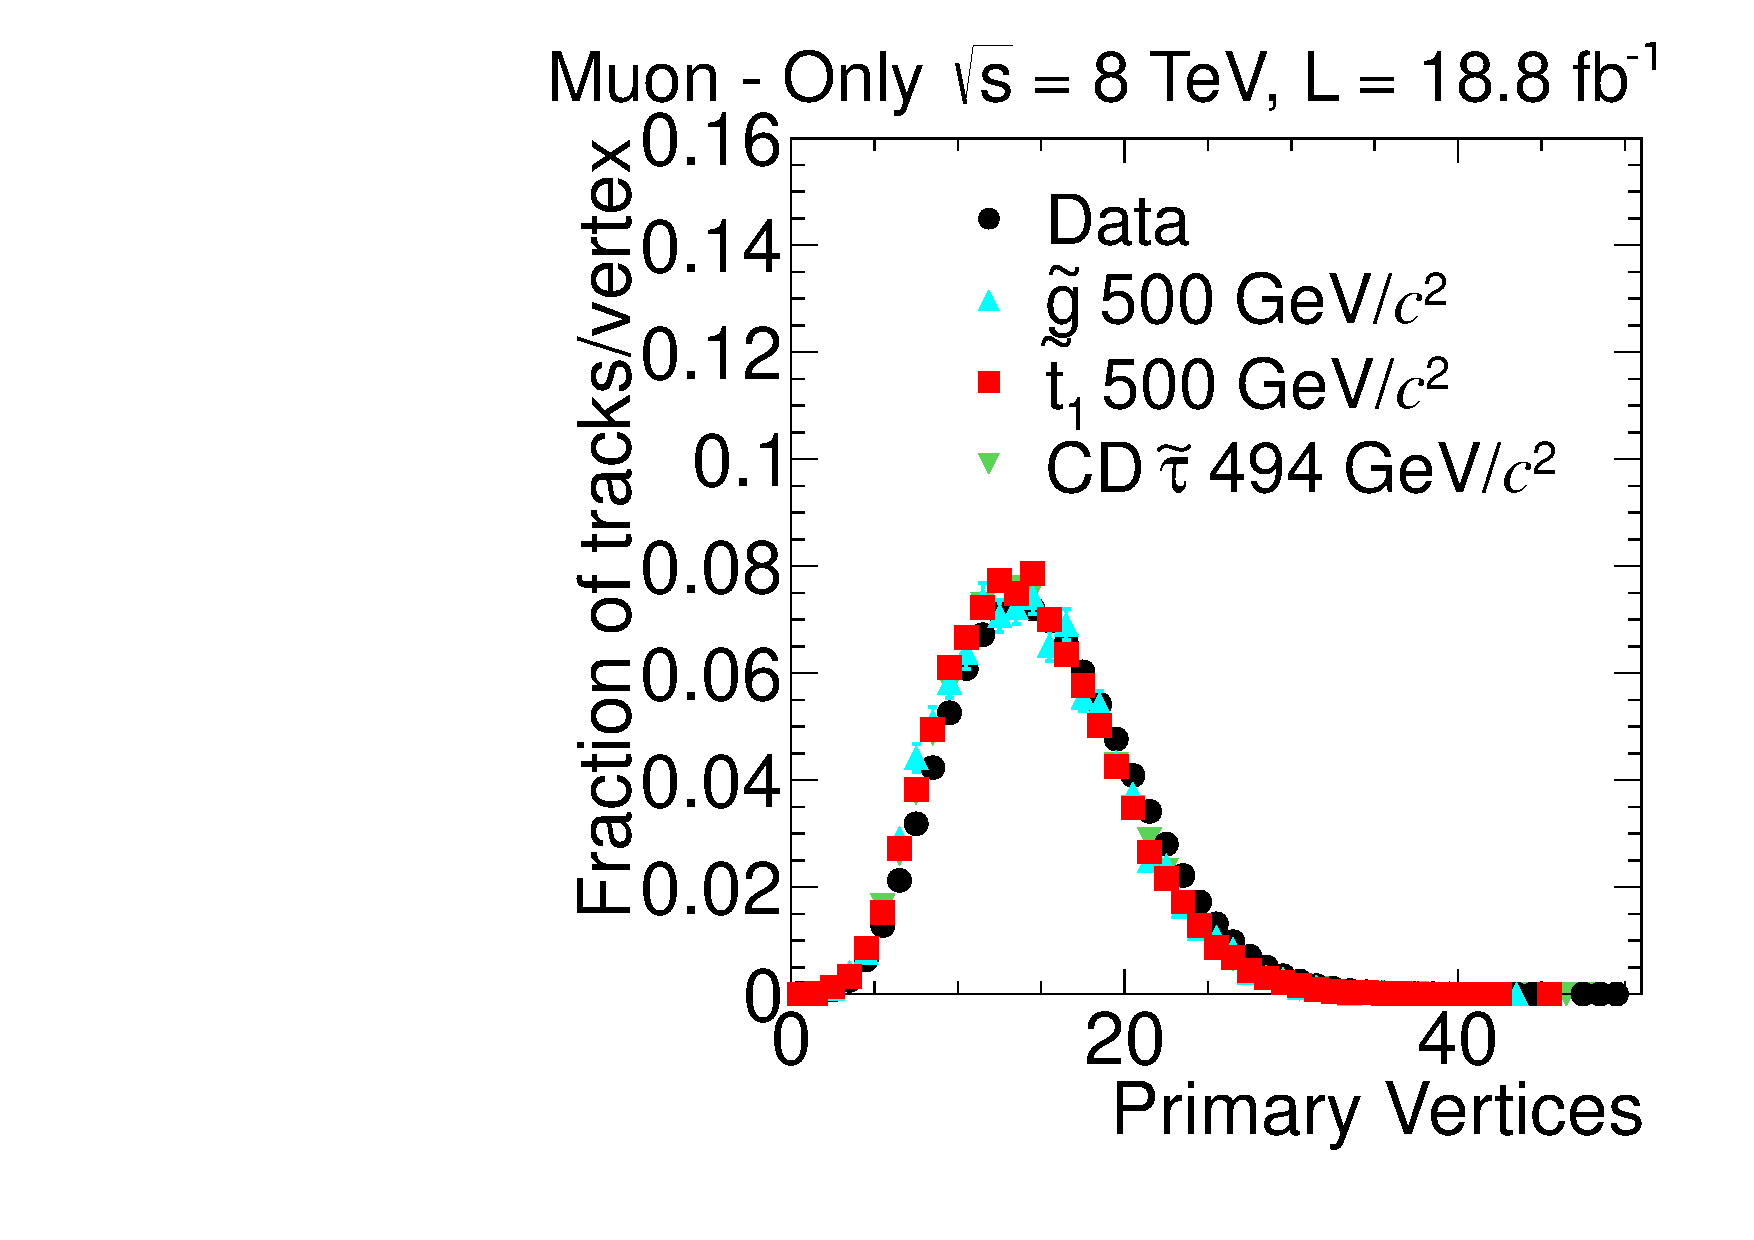
\includegraphics[clip=true, trim=0.0cm 0cm 3.0cm 0cm, width=0.44\textwidth]{figures/muonly/Selection_Comp_Signal_8TeV_PV_BS}
      \renewcommand\baselinestretch{1}\caption[Gluino1200f100 System Pt vs MET]
        {Distribution of number of vertices in Data and various MC samples
        }
      \renewcommand\baselinestretch{\@spacing}
      \label{fig:PV}
  \end{center}
\end{figure}

\section{Trigger \label{sec:trigger}}
All events used in the search are required to be triggered by one of three algorithms. The algorithms require a track to be found
and/or missing transverse energy, PFMET, as calculated by the particle flow algorithm~\cite{CMS-PAS-JME-10-003}. 

The particle flow algorithm attempts
to reconstruct all particles in an event, then calculates PFMET as the negative vector sum of the transverse momentum of the particles. As the proton-proton collision occurs
at rest in the transverse plane, PFMET is meant to represent the vector sum of all particles not found by the particle flow algorithm. For most CMS analyses PFMET is created
by either the limited detector response in finding all tracks in an event and determining their momentum or from neutral particles in the event which leave no signals
in the detector. These neutral particles could be neutrinos from the standard model or new neutral particles created in a BSM theory such as supersymmetry. 

For HSCP the
PFMET often arises because of details of the particle flow algorithm. The algorithm assumes SM particles and rejects tracks that do not conform to the properties expected
of a SM particle. Two types of possible HSCP tracks are rejected by the algorithm. The first is tracks reconstructed only in the muon system. The only SM particles that
are expected to reach the muon system are muons and muons should have a matching track in the inner tracker. HSCP produced neutral then acquiring charge as they propagate
through CMS usually would only have a track in the muon system and as such would not be included in the PFMET calculation. 

The second is tracks produced charged but
becoming neutral as they propagate through CMS.
The particle flow algorithm rejects tracks reconstructed only in the inner tracker that have a track $p_T$ much larger
than the associated energy deposited in the calorimeter. As an HSCP only deposits approximately 10GeV of energy in the calorimeter and normally have $> 100$GeV of momentum
HSCP neutral in the muon system will likely be rejected. 

These two effects lead to PFMET in HSCP events to be roughly equal to the vector sum of any HSCP neutral in
either the muon system or the inner tracker, less however much energy they deposit in the muon system. This effect can be seen in Figures~\ref{fig:SystPtTrigger} 
and~\ref{fig:SystPtTriggerN} which compare the di-HSCP system with online PFMET in events with at least 150 GeV of online PFMET.

\begin{figure}
  \begin{center}
      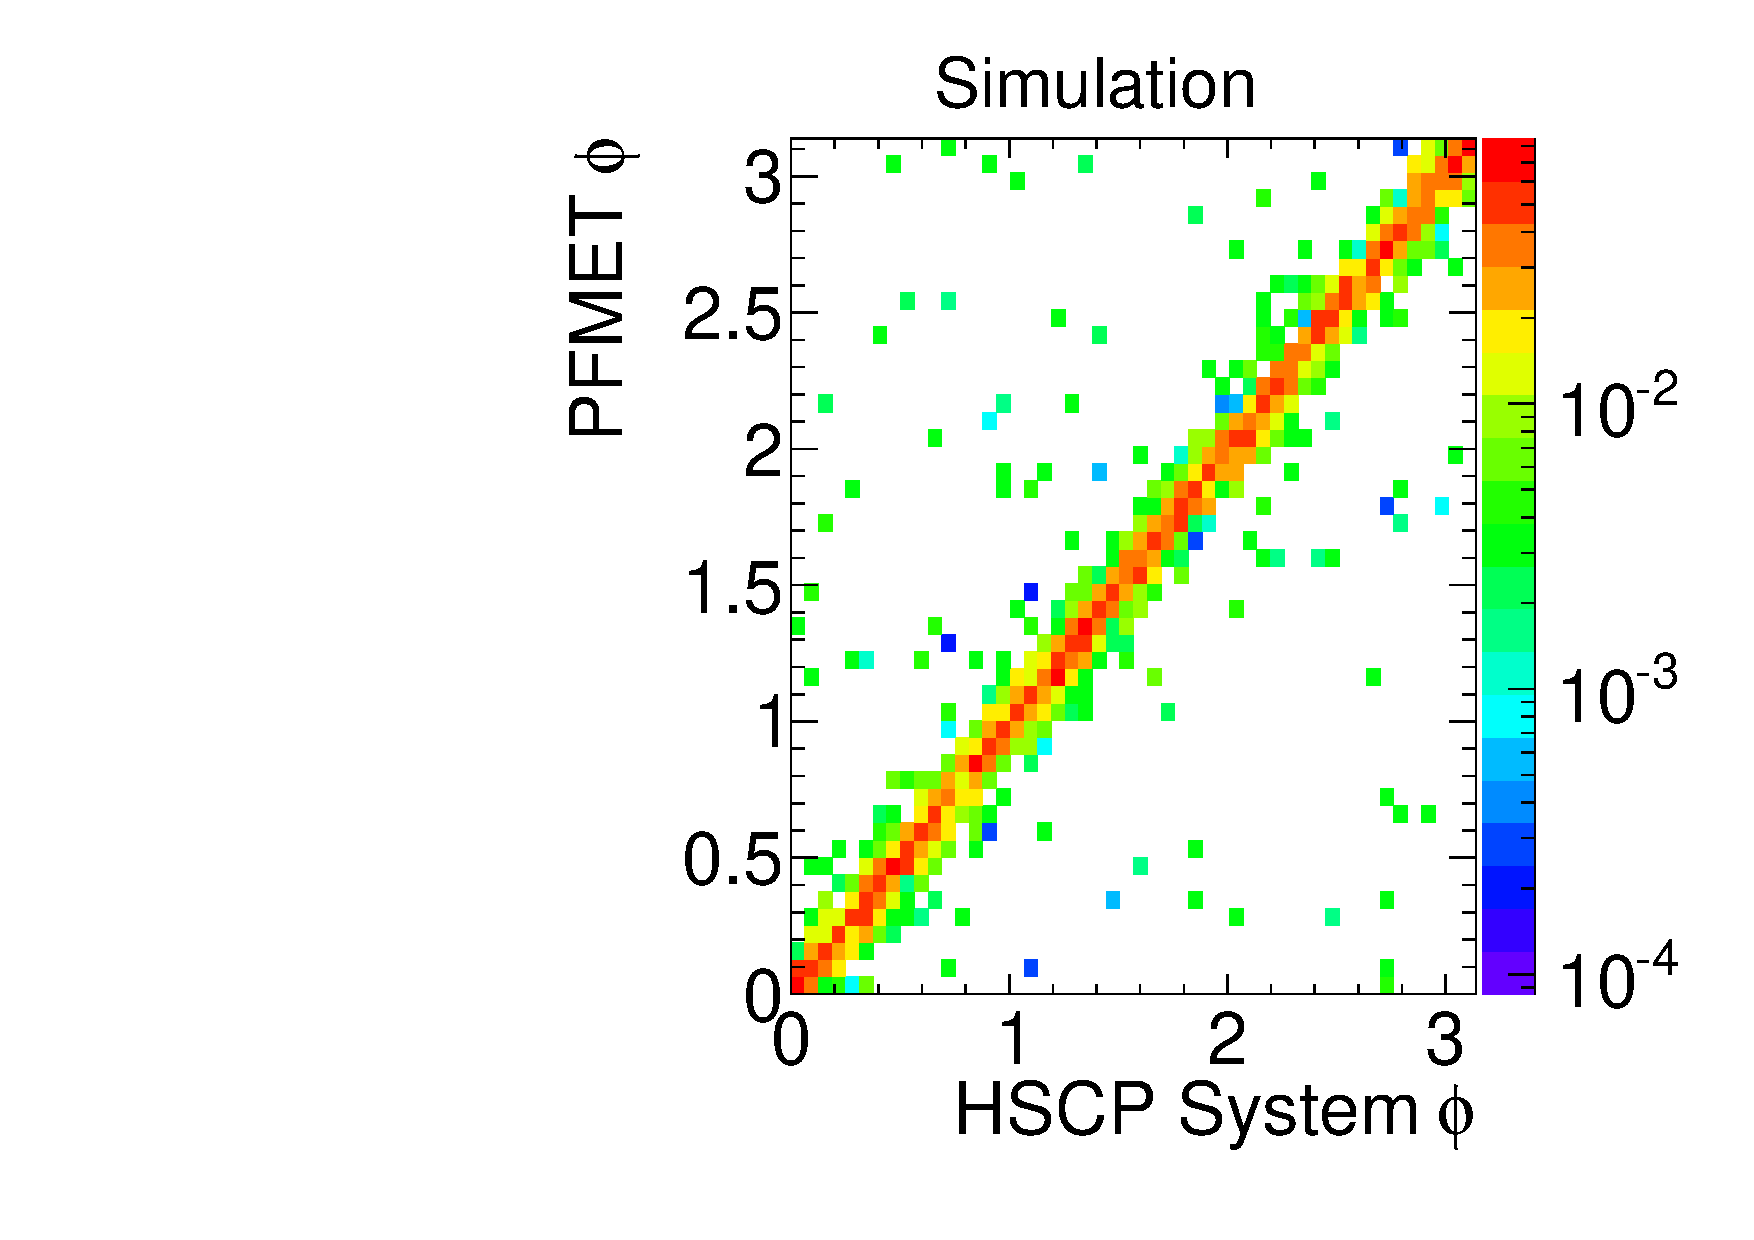
\includegraphics[clip=true, trim=0.0cm 0cm 3.0cm 0cm, width=0.44\textwidth]{figures/search/Gluino_8TeV_M1200_f100SystPhiMET}
      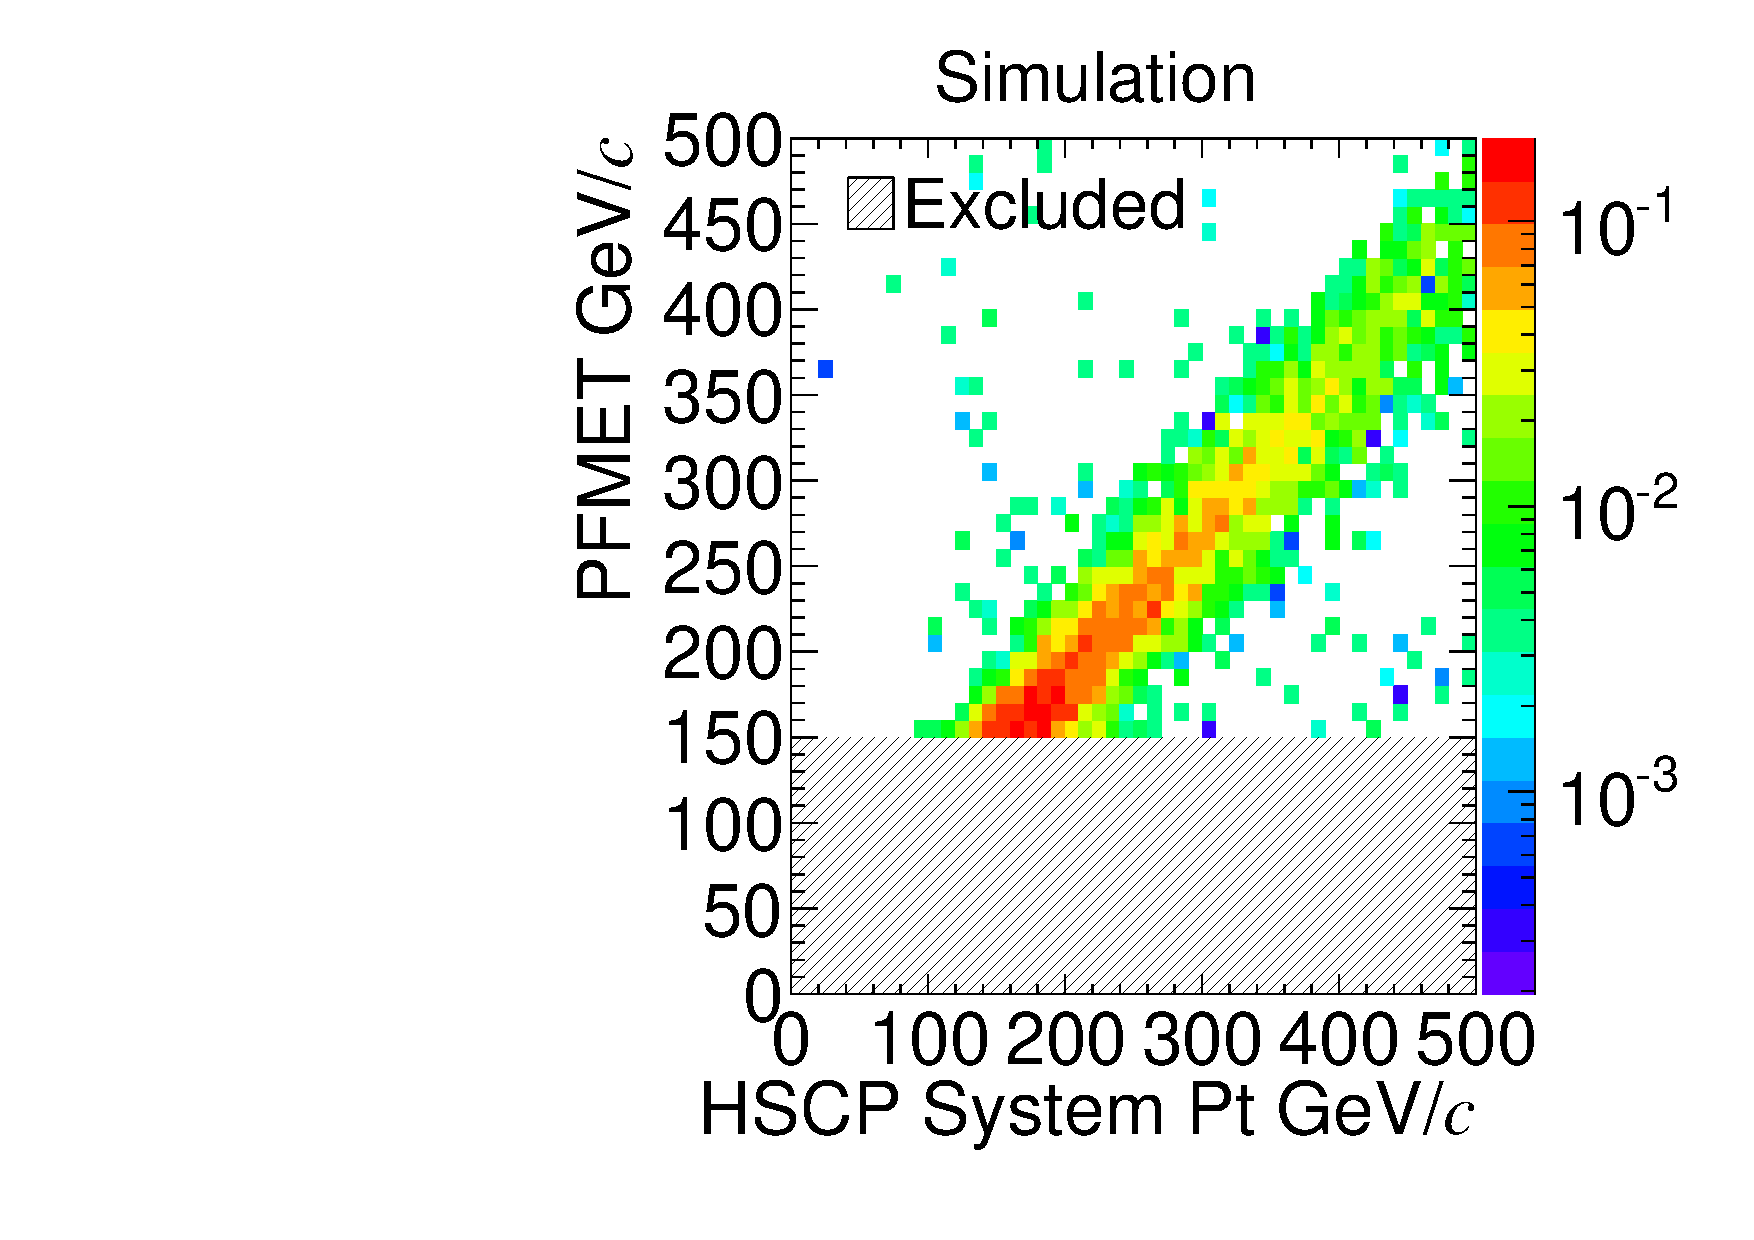
\includegraphics[clip=true, trim=0.0cm 0cm 3.0cm 0cm, width=0.44\textwidth]{figures/search/Gluino_8TeV_M1200_f100SystPtMET} \\
      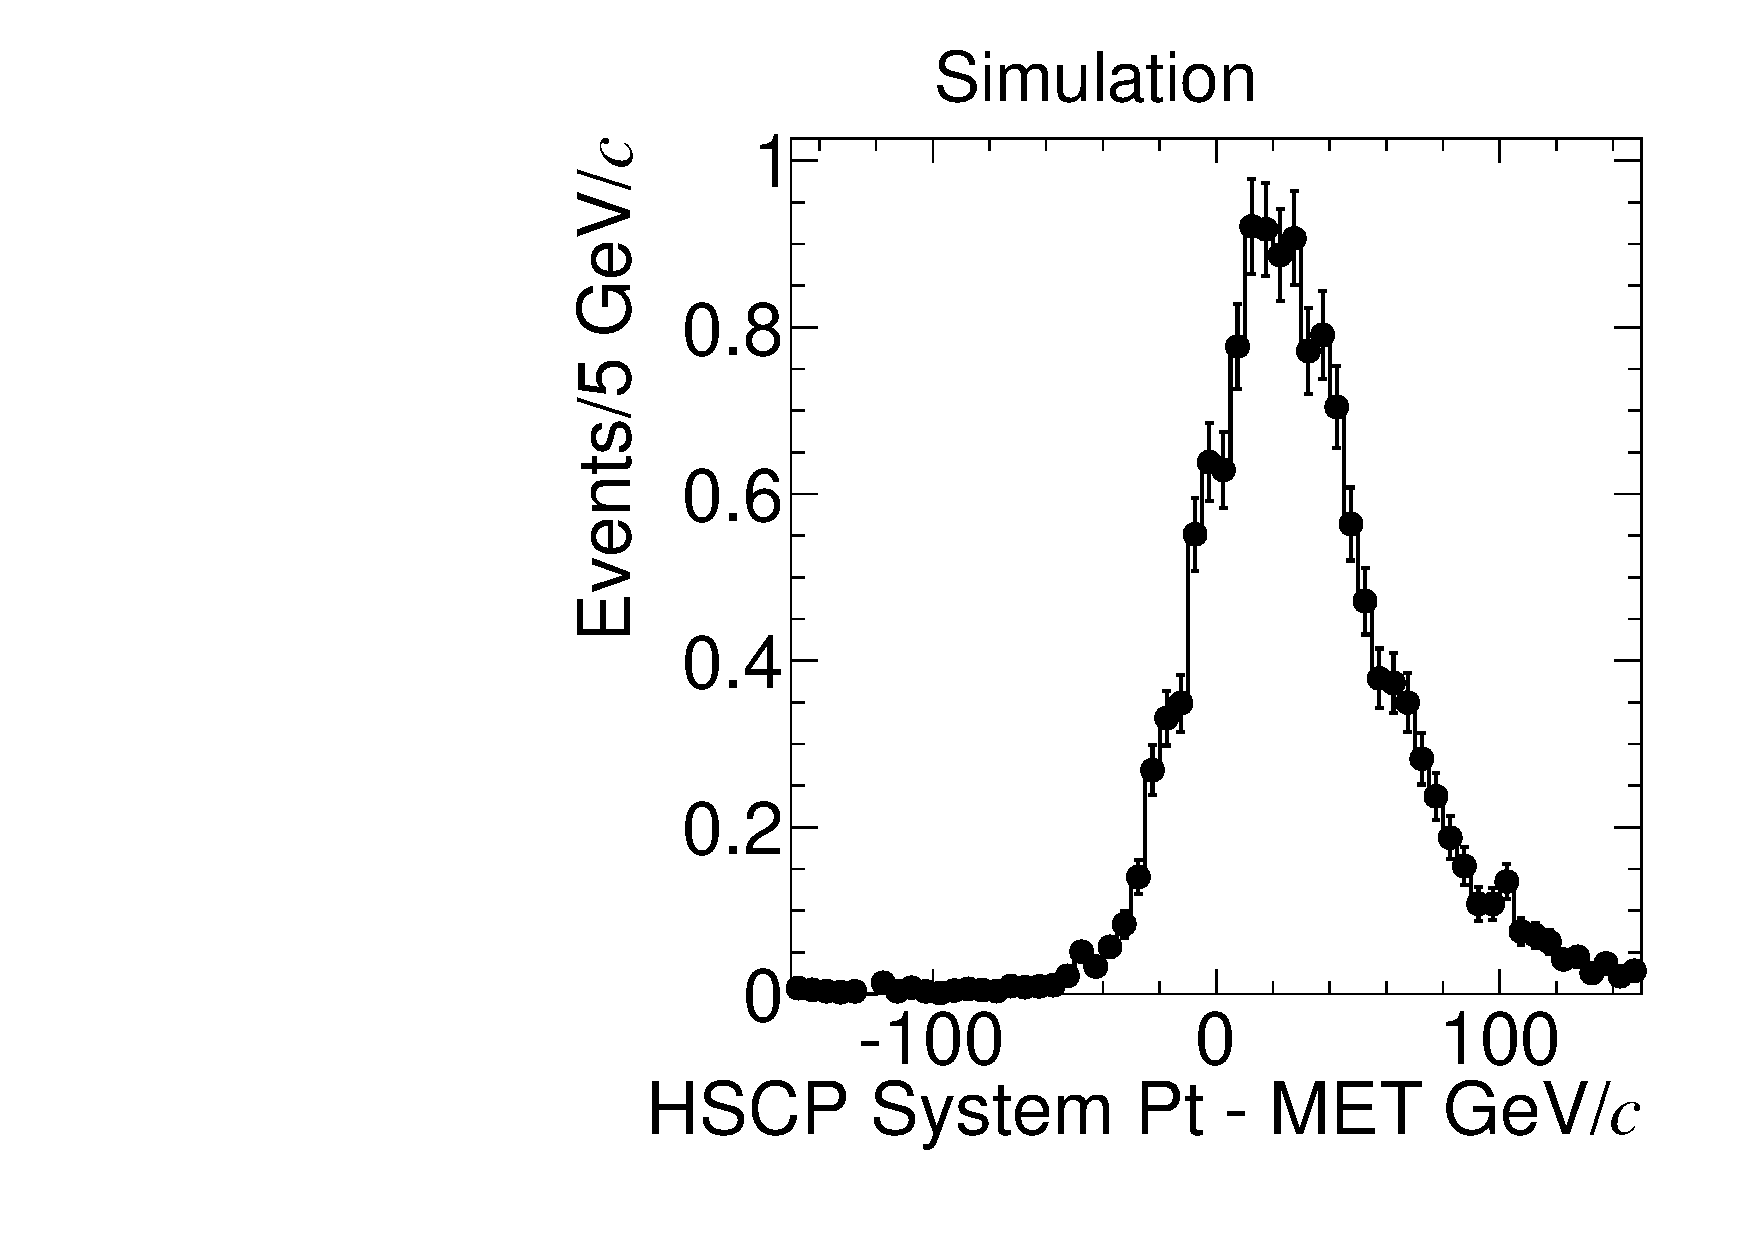
\includegraphics[clip=true, trim=0.0cm 0cm 3.0cm 0cm, width=0.44\textwidth]{figures/search/Gluino_8TeV_M1200_f100SystPtDiffMET}
      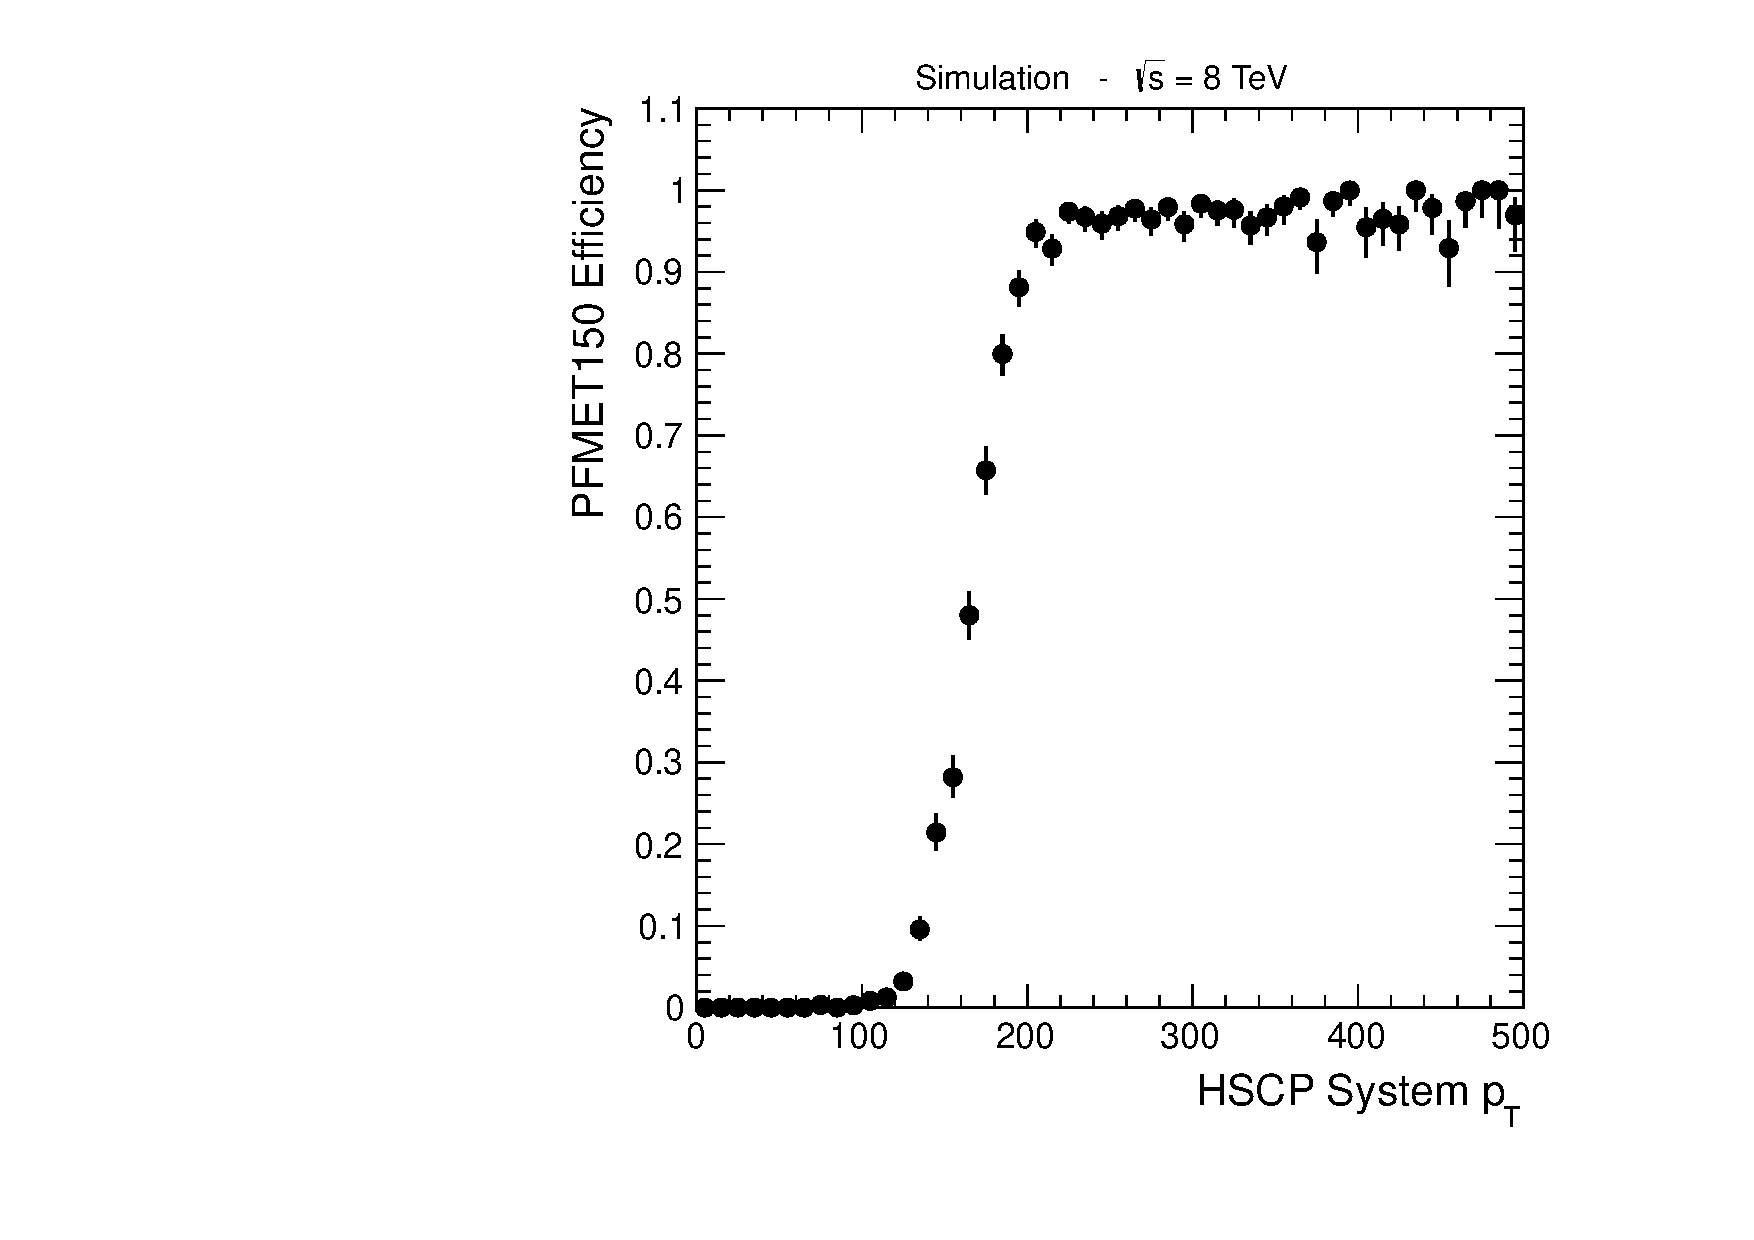
\includegraphics[clip=true, trim=0.0cm 0cm 3.0cm 0cm, width=0.44\textwidth]{figures/search/Gluino_8TeV_M1200_f100SystPtEff}
      \renewcommand\baselinestretch{1}\caption[Gluino1200f100 System Pt vs MET]
        {Comparison of di-HSCP system with online PFMET for a 1200 GeV Gluino $f=1.0$ sample in events with at least 150 GeV of online PFMET. 
         Top Left: Online PFMET $\phi$ versus di-HSCP system $\phi.$ Top Right: Online PFMET value versus di-HSCP system $p_T$. 
         Bottom Left: Difference between di-HSCP system $p_T$ and online PFMET value.
         Bottom Right: Probability to have online PFMET greater than 150 versus di-HSCP system $p_T$.
        }
      \renewcommand\baselinestretch{\@spacing}
      \label{fig:SystPtTrigger}
  \end{center}
\end{figure}

\begin{figure}
  \begin{center}
      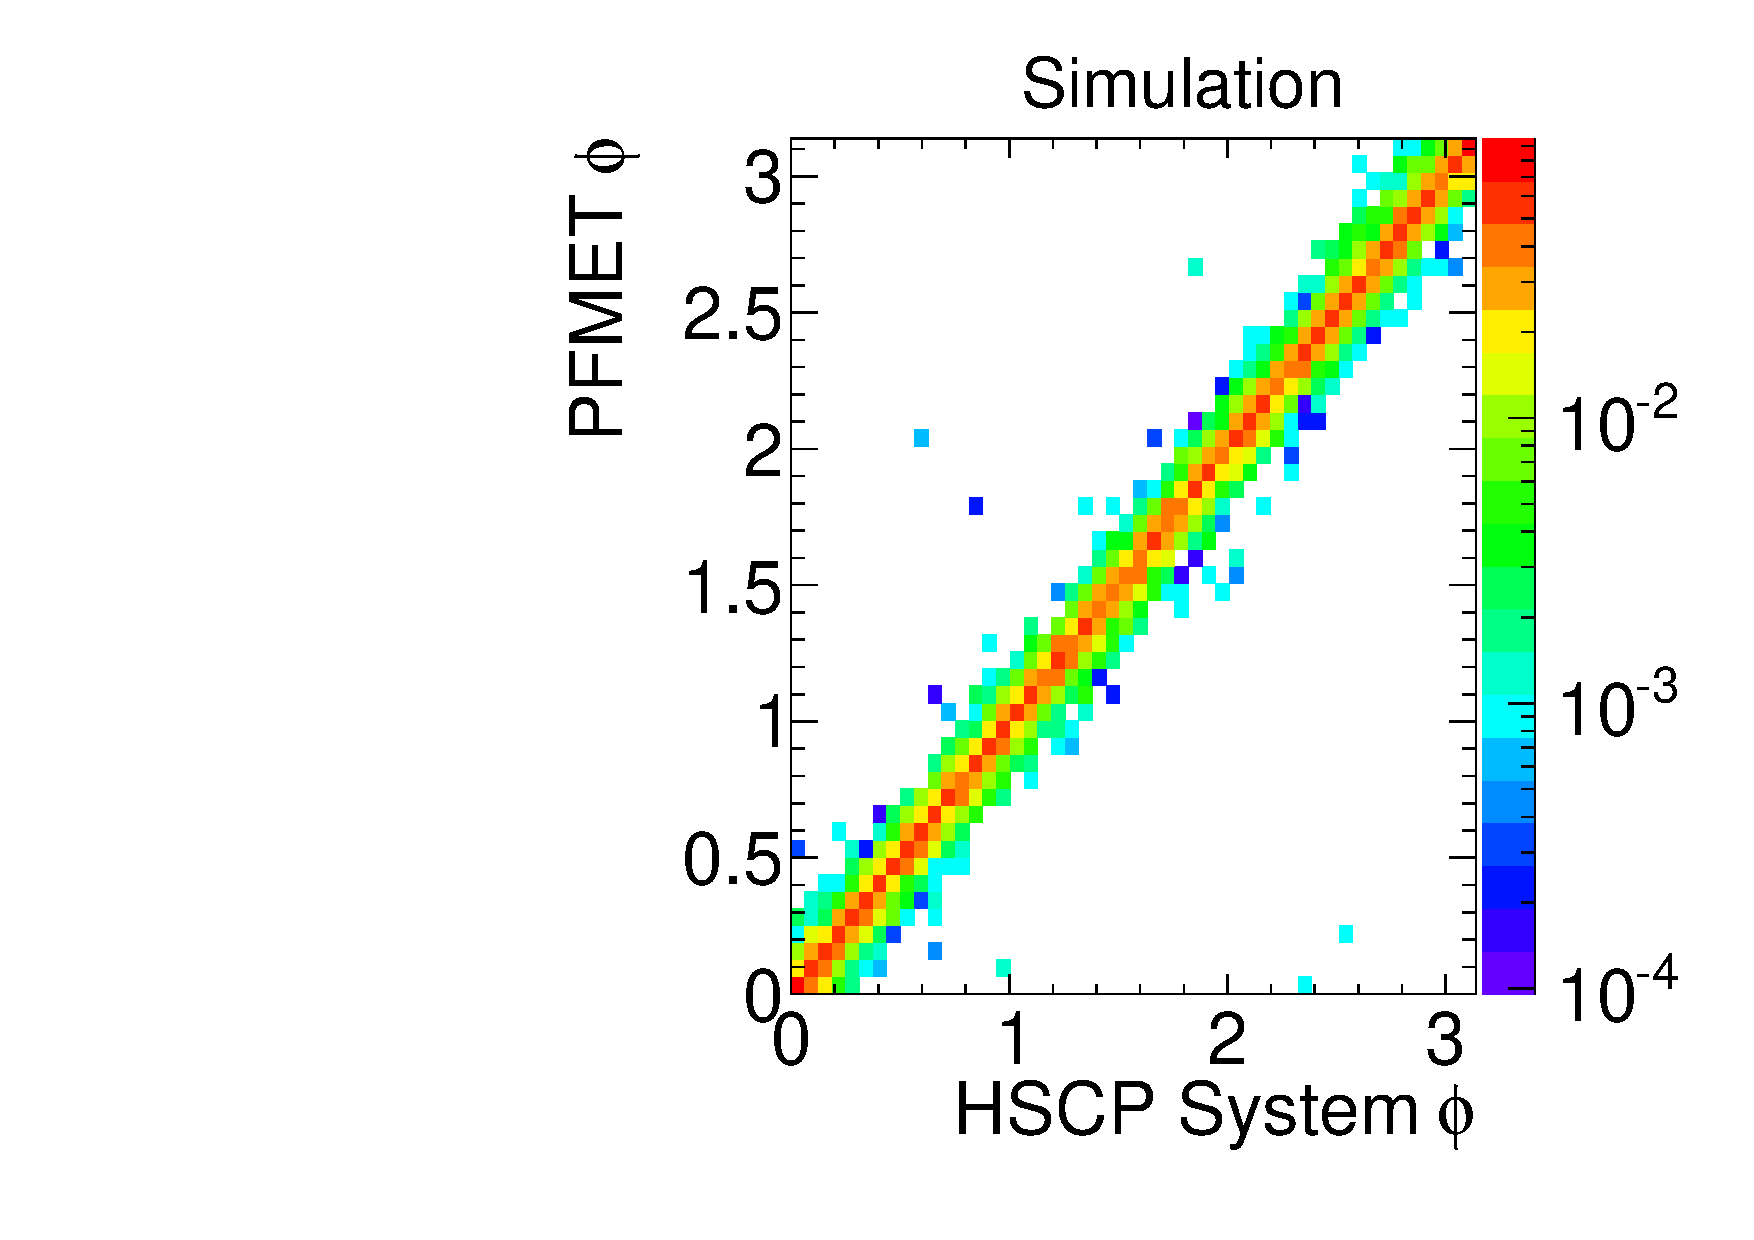
\includegraphics[clip=true, trim=0.0cm 0cm 3.0cm 0cm, width=0.44\textwidth]{figures/search/Gluino_8TeV_M1200N_f10SystPhiMET}
      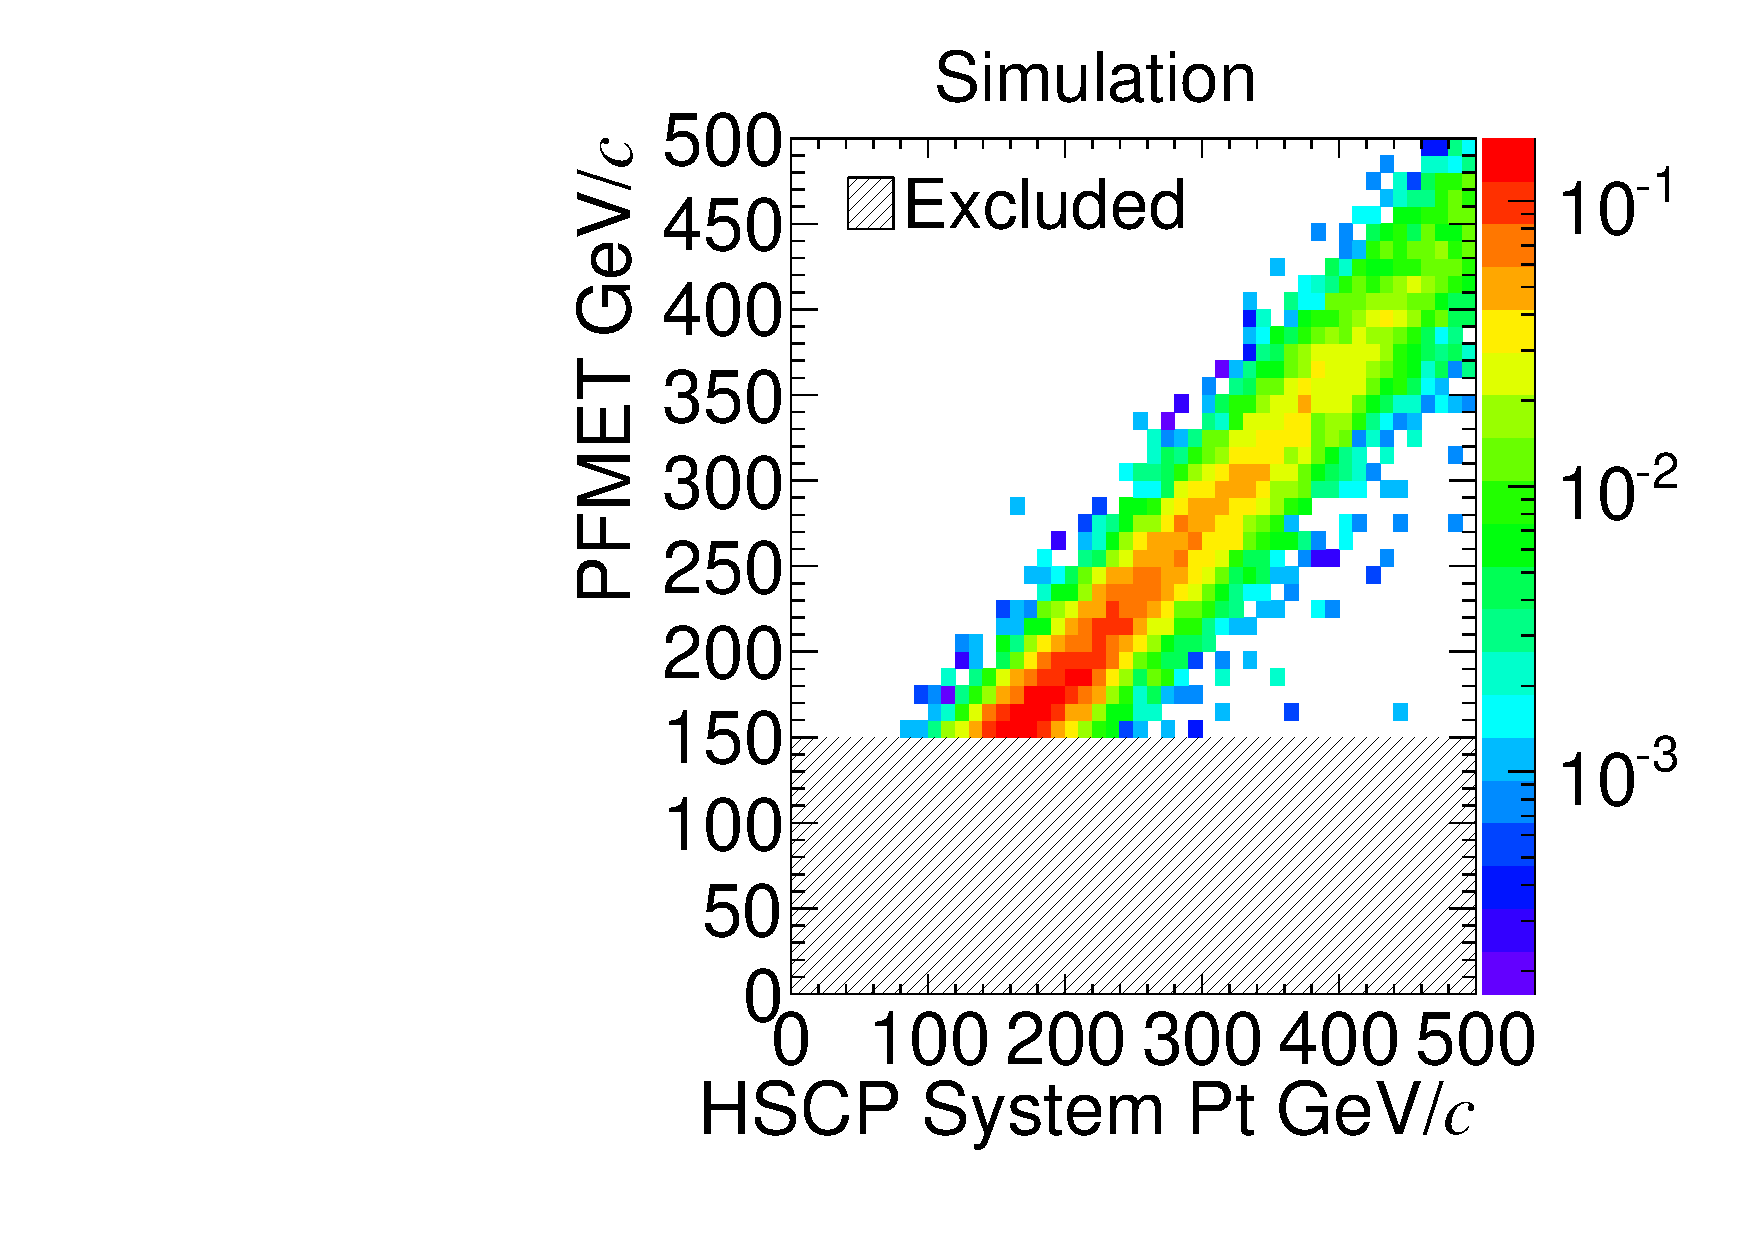
\includegraphics[clip=true, trim=0.0cm 0cm 3.0cm 0cm, width=0.44\textwidth]{figures/search/Gluino_8TeV_M1200N_f10SystPtMET} \\
      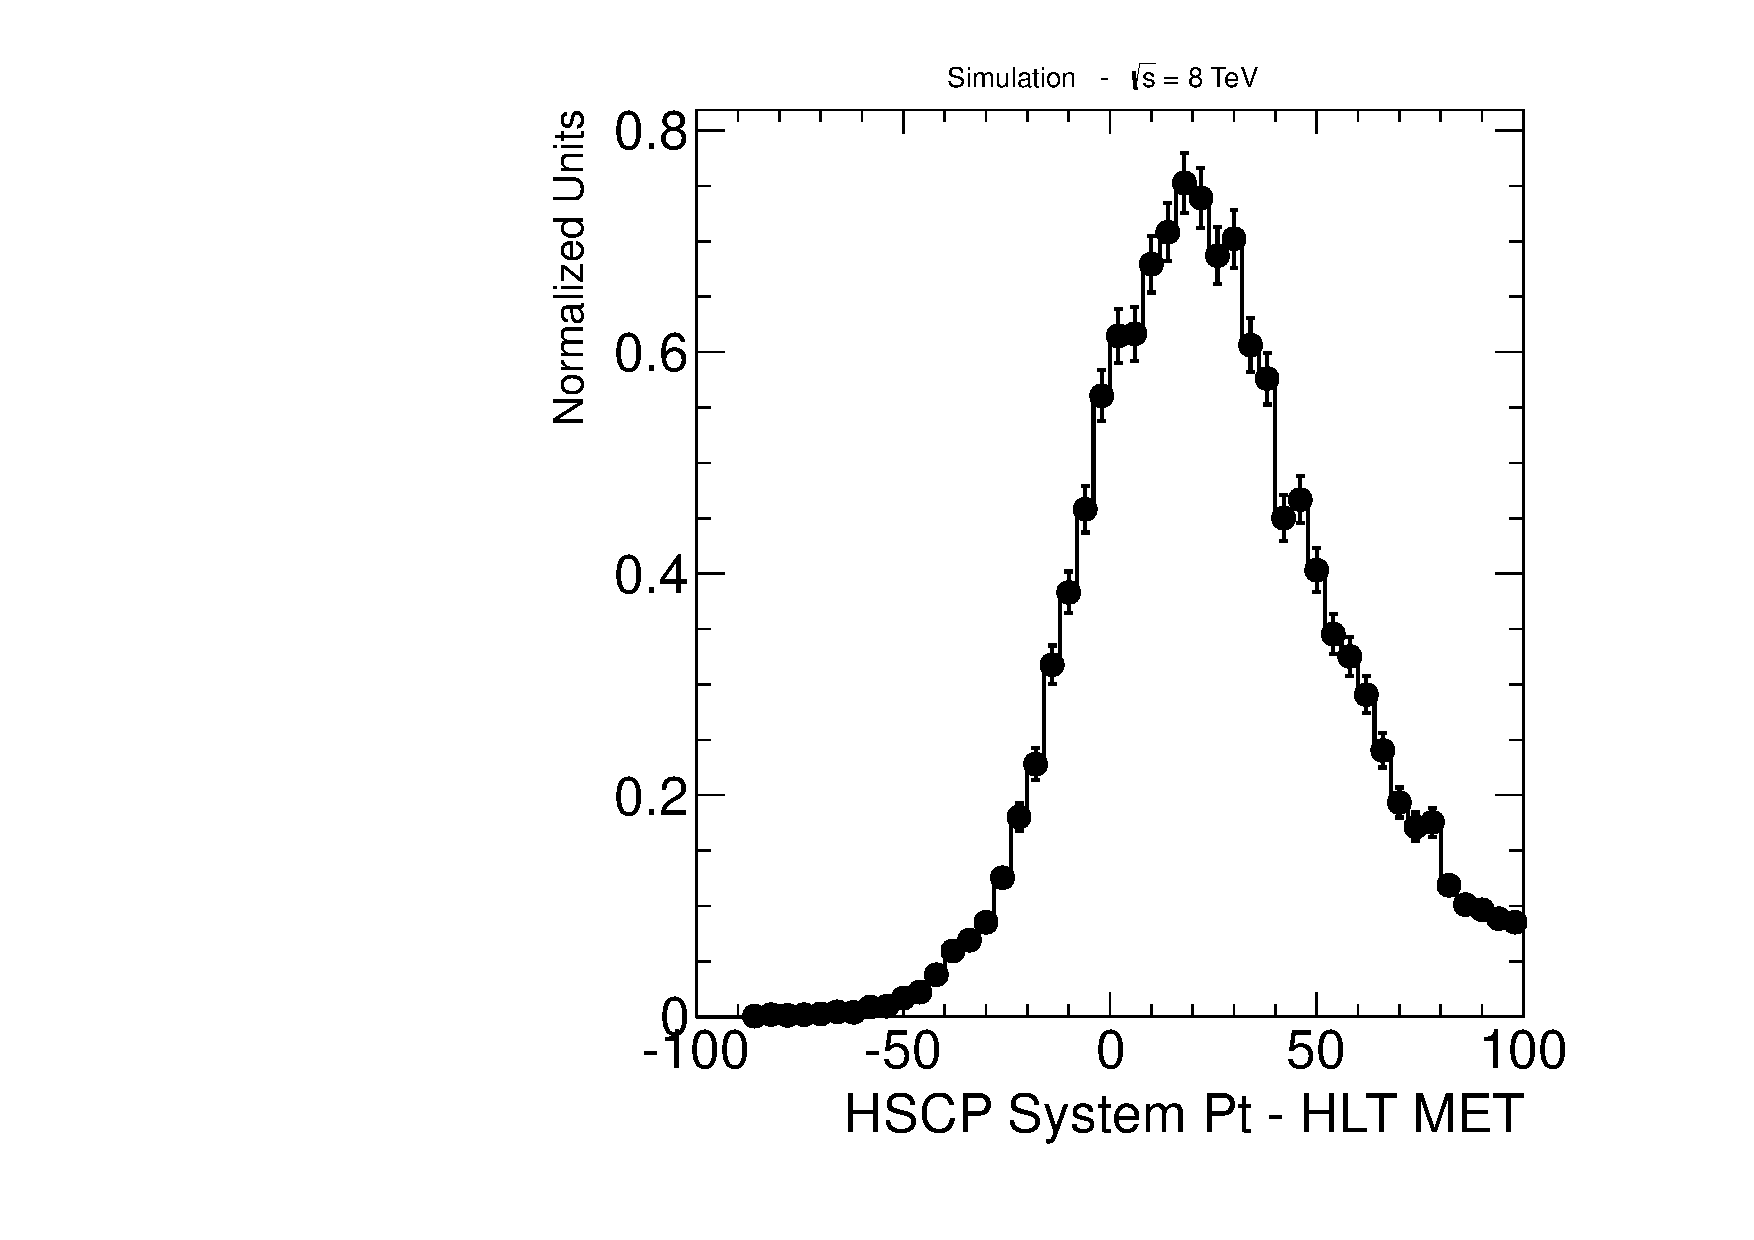
\includegraphics[clip=true, trim=0.0cm 0cm 3.0cm 0cm, width=0.44\textwidth]{figures/search/Gluino_8TeV_M1200N_f10SystPtDiffMET}
      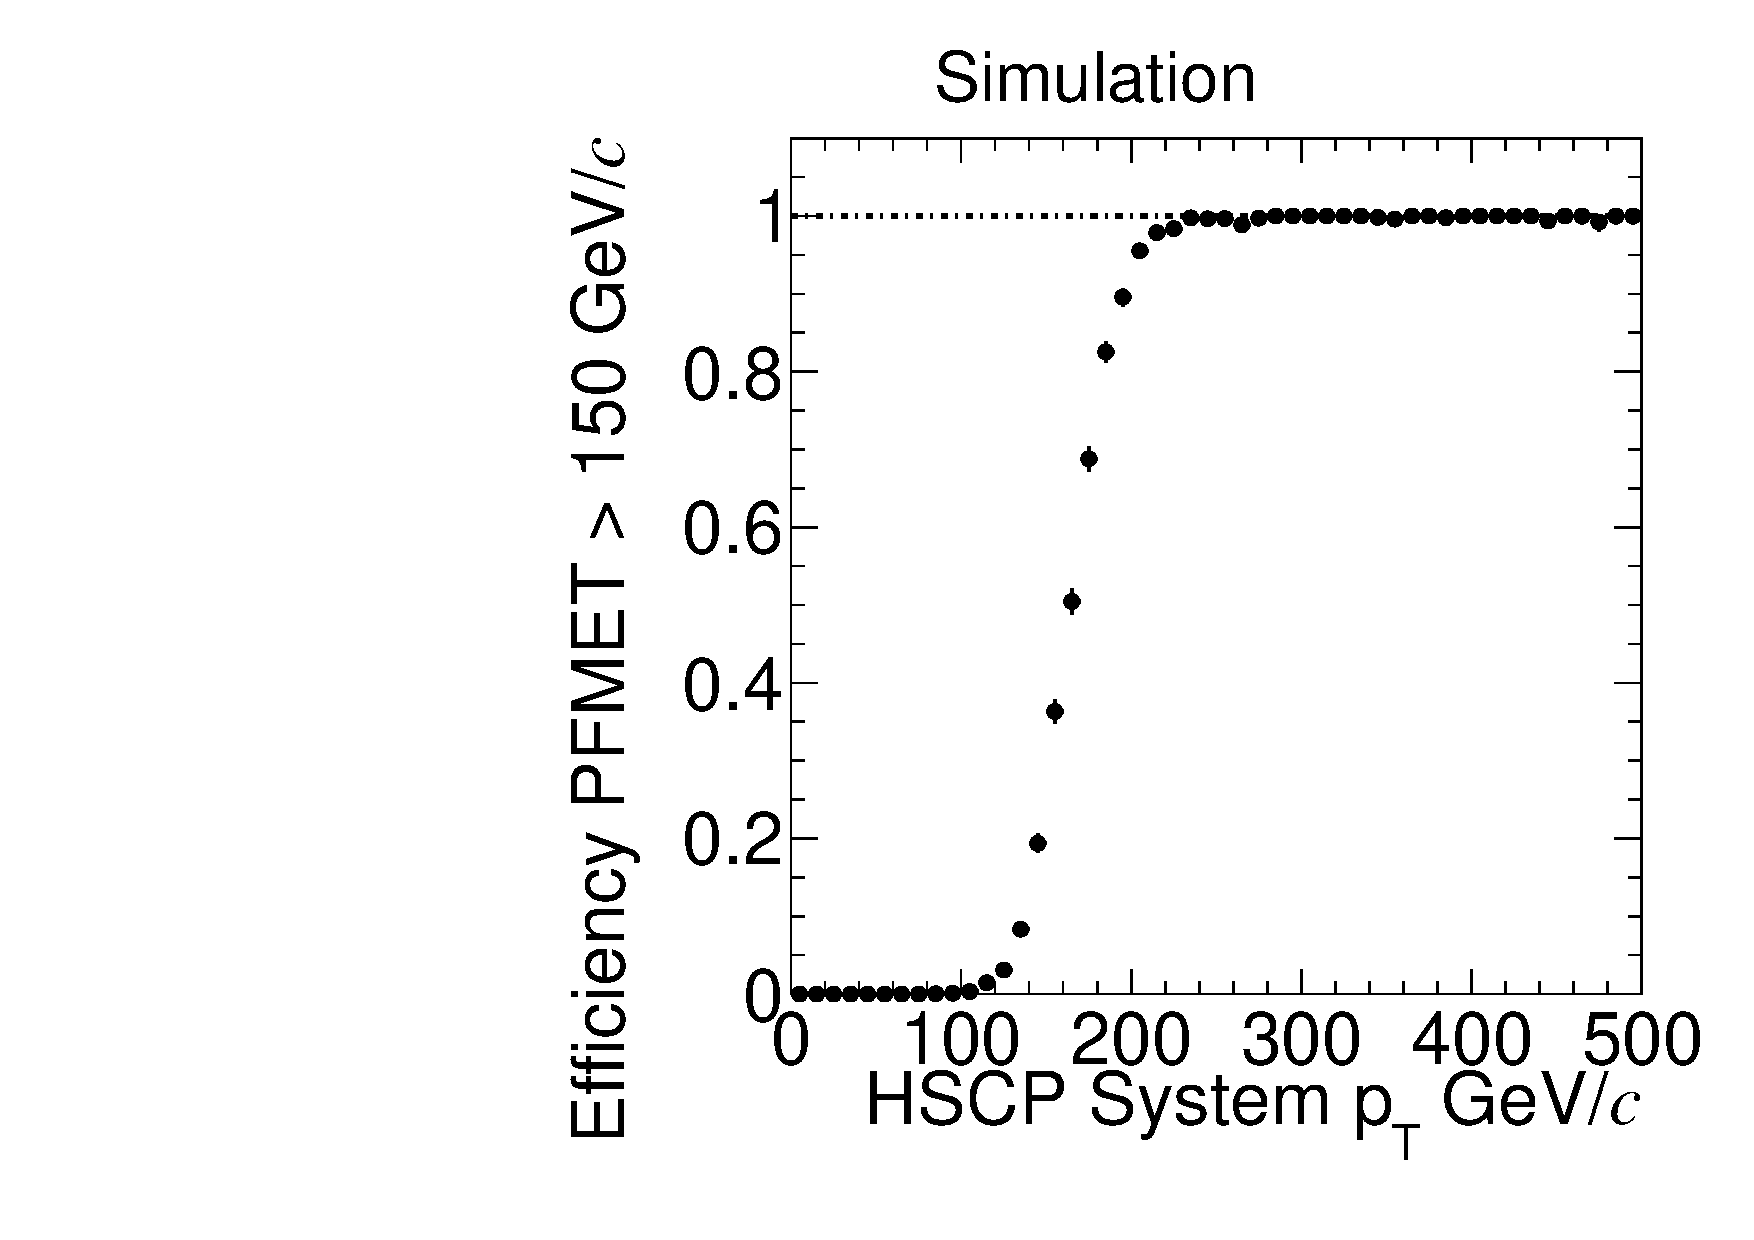
\includegraphics[clip=true, trim=0.0cm 0cm 3.0cm 0cm, width=0.44\textwidth]{figures/search/Gluino_8TeV_M1200N_f10SystPtEff}
      \renewcommand\baselinestretch{1}\caption[Gluino1200f100 System Pt vs MET]
      {Comparison of di-HSCP system with online PFMET for a charge suppressed 1200 GeV Gluino $f=0.1$ sample in events with at least 150 GeV of online PFMET.
         Top Left: Online PFMET $\phi$ versus di-HSCP system $\phi.$ Top Right: Online PFMET value versus di-HSCP system $p_T$.
         Bottom Left: Difference between di-HSCP system $p_T$ and online PFMET value.
         Bottom Right: Probability to have online PFMET greater than 150 versus di-HSCP system $p_T$.
        }
      \renewcommand\baselinestretch{\@spacing}
      \label{fig:SystPtTriggerN}
  \end{center}
\end{figure}

One trigger issue unique to slow moving particles is the acceptance of the L1 trigger. If an HSCP arrives in the muon system too late it can trigger the
readout of the wrong bunch crossing. As most of the CMS subdetectors, though not the muon system, are designed to not readout data coming from adjacent bunch crossings
the data from the correct bunch crossing would be lost. To help deal with this members of the CMS L1 trigger team developed a special configuration of the
RPC L1 trigger to partially recover HSCP that arrive in the muon system in the bunch crossing following the crossing they were produced in.
The configuration creates a duplicate copy of all RPC hits and sends them to the muon trigger in the bunch crossing immediately preceding the arrival of the hits. 
This allows for HSCP that
arrive in the RPCs 0.5 -- 1.5 bunch crossings later than a collision muon would to still trigger the readout of the correct event. For particles that arrive in the RPC
in the correct bunch crossing a coincidence with the LHC beam crossing through the machine is required to prevent the readout of the previous event. This configuration
was possible for 2012 running as the proton bunches were separated by 50ns despite having 25ns wide bunch crossing windows.

The first of the three algorithms used requires both a track to be found in the muon system with $p_T > 70$GeV and $|\eta| < 2.1$ as well as MET $ > 55$GeV. 
For the first 700$pb^{-1}$ of 2012 running the threshold was at 65GeV. The signal samples are weighted
to account for the amount data taken at each threshold. Events collected with this trigger are only used
in the \muononly\ analysis.
The second algorithm requires a track matched in both the inner tracker
and muon system to be found by the HLT with $p_T > 40$GeV and $|\eta| < 2.1$. The only requirement for the third algorithm is PFMET $ > 150$GeV.
The second and third algorithms are used in all the analyses.

The decision to use the pure PFMET trigger even though a muon signature is required offline is prompted by the late arrival of the HSCPs in the muon system.
Even with the RPC configuration described above very slow moving HSCP can trigger the readout of the wrong event but still be reconstructed offline
if the event has been triggered by the pure MET trigger. This can be seen in Figure~\ref{fig:TriggerEffVsBetaGl} which shows the trigger efficiency versus $\beta$
with and without the pure MET trigger. Thus using the pure MET trigger allows the search to probe lower $\beta$ particles. 

As color charged $R$-hadron can be neutral
while traversing CMS or arrive so late to the muon system that they are not able to be reconstructed offline an effective detector acceptance is defined 
that at least one HSCP be reconstructed offline. Thus Figure~\ref{fig:TriggerEffVsBetaGl} shows the efficiency requiring an HSCP be reconstructed as a a stand alone track,
as in the \muononly\ analysis, and as a global track, as in the the \tktof\ analysis.

\begin{figure}
\centering
  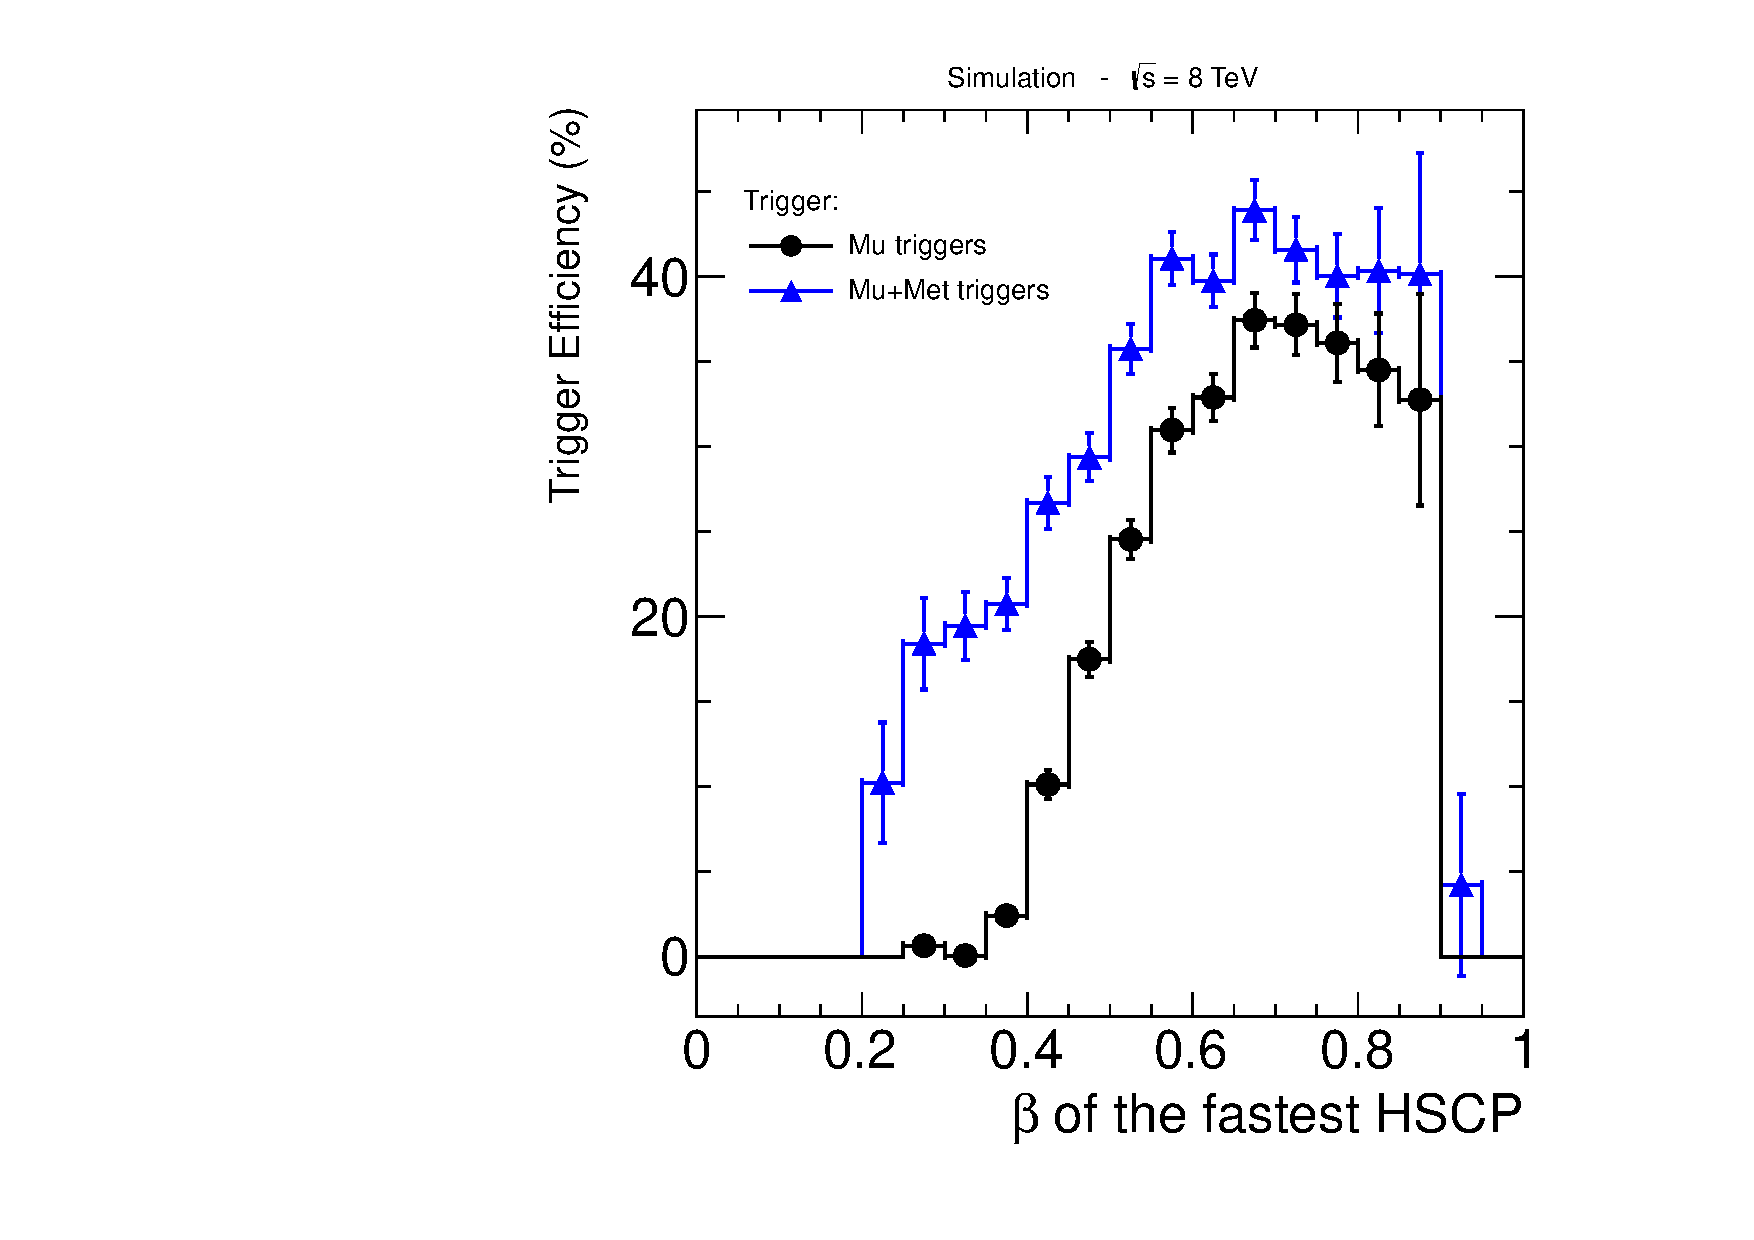
\includegraphics[clip=true, trim=0.0cm 0cm 3.0cm 0cm, width=0.32\textwidth]{figures/search/Gluino_8TeV_M1200_f100MatchedSA}
  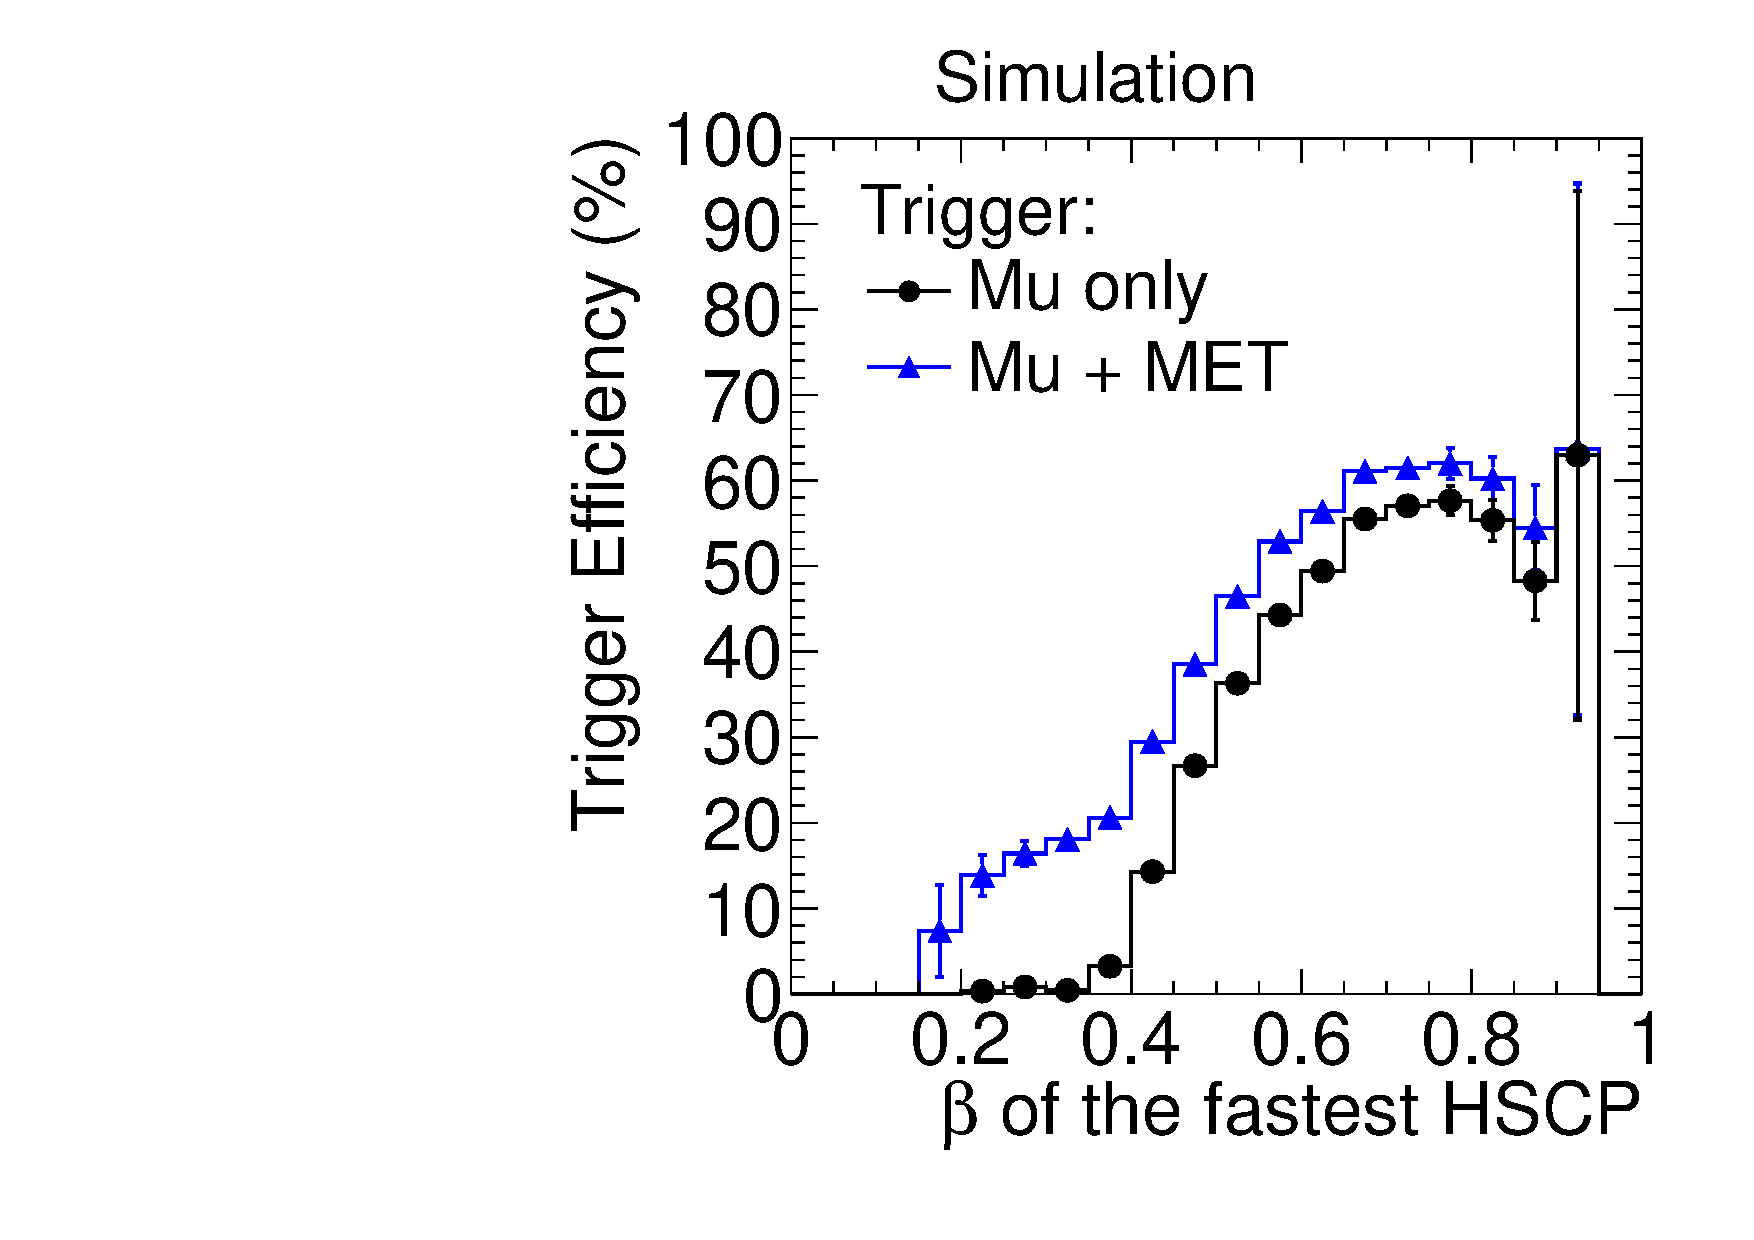
\includegraphics[clip=true, trim=0.0cm 0cm 3.0cm 0cm, width=0.32\textwidth]{figures/search/Gluino_8TeV_M1200_f10MatchedSA}
  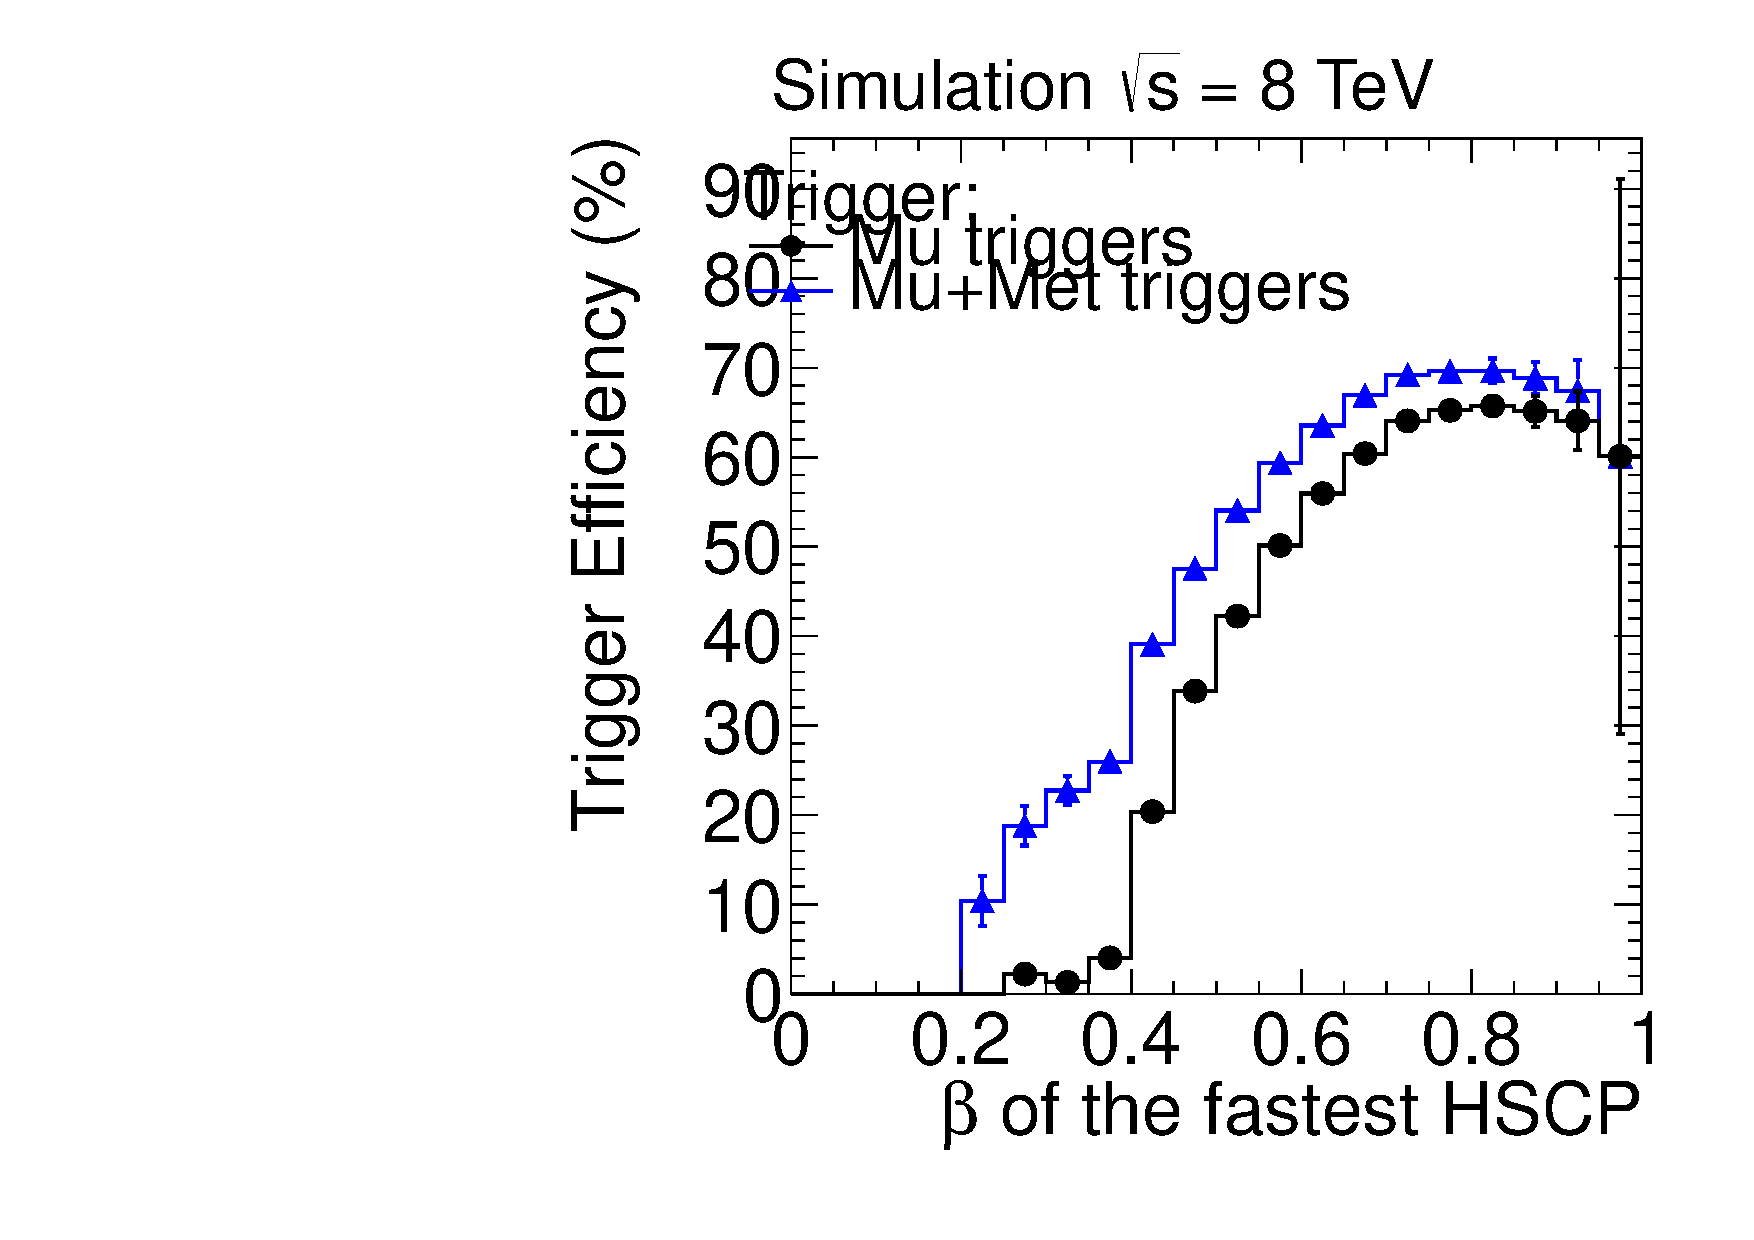
\includegraphics[clip=true, trim=0.0cm 0cm 3.0cm 0cm, width=0.32\textwidth]{figures/search/Stop_8TeV_M800MatchedSA}
  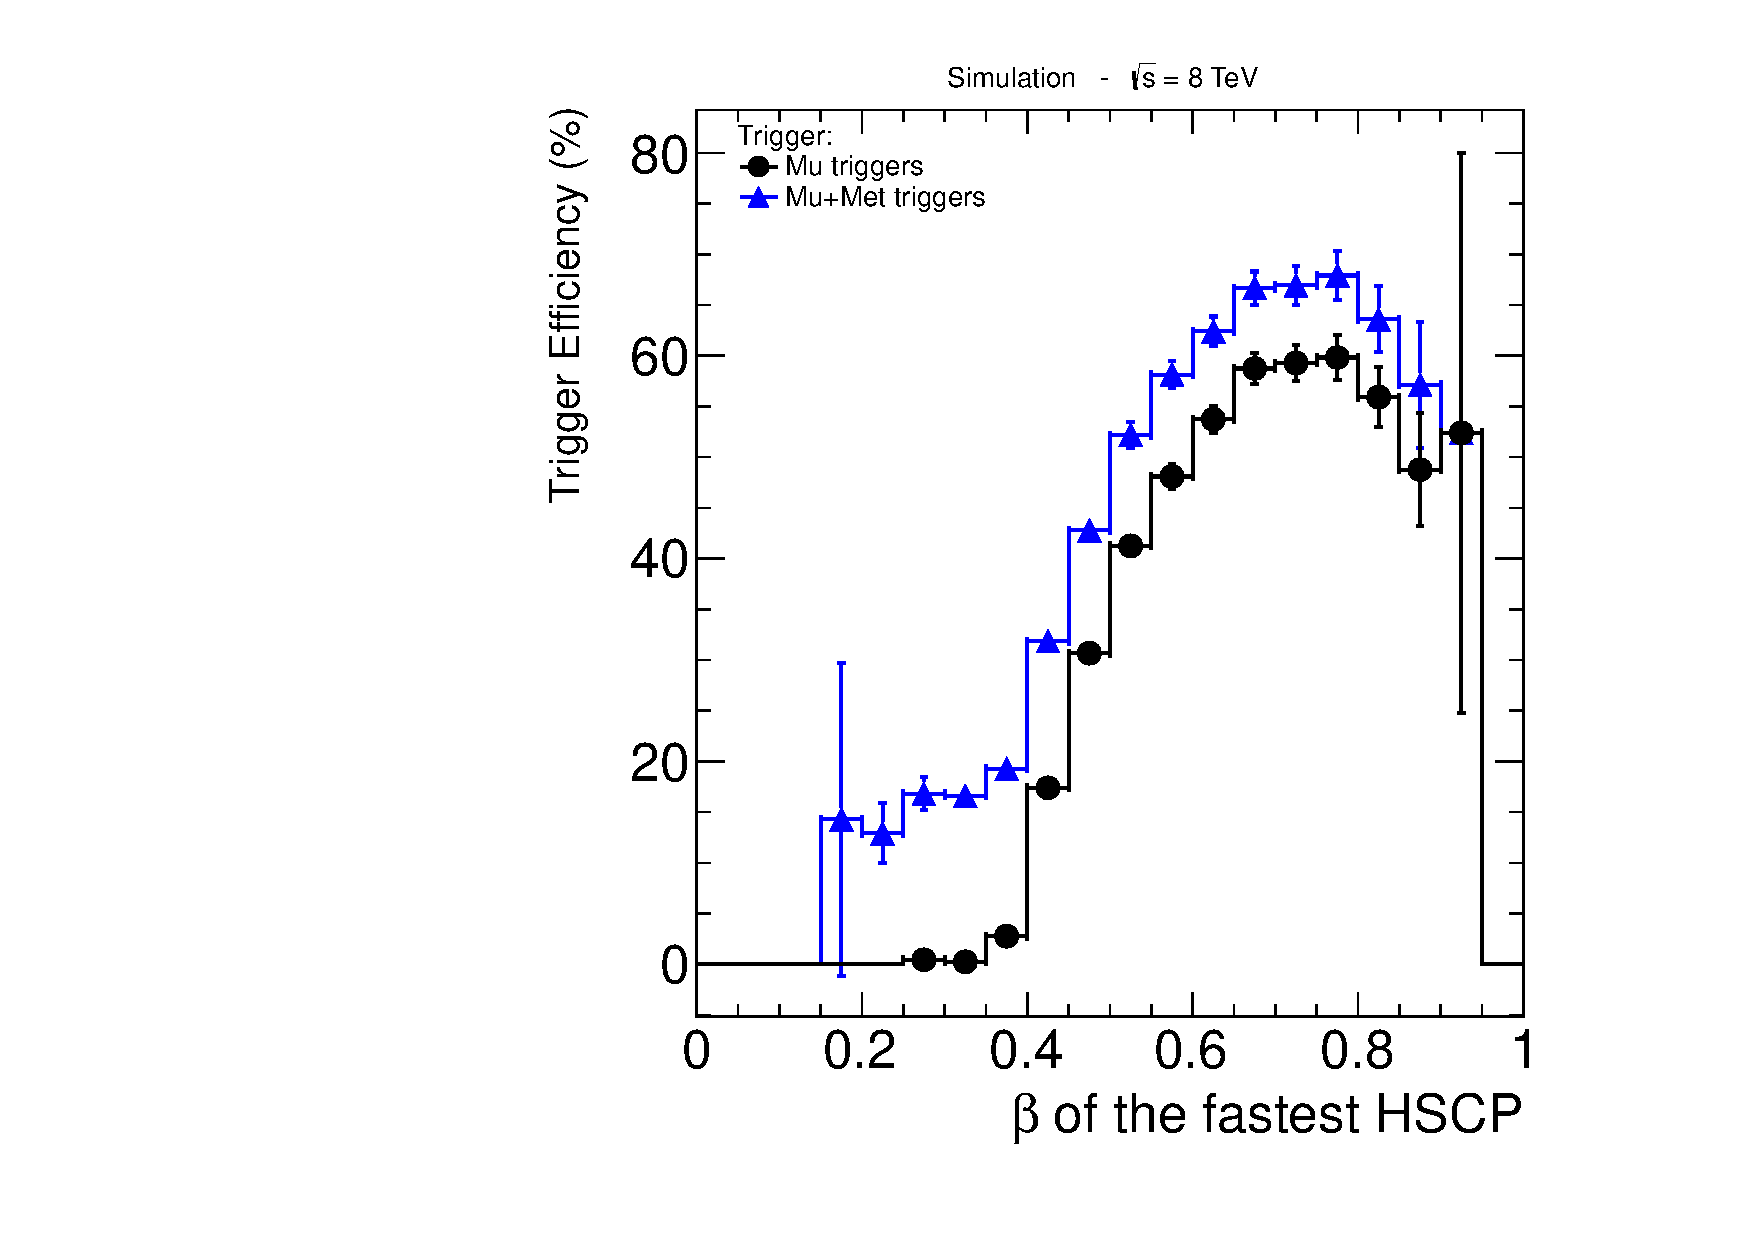
\includegraphics[clip=true, trim=0.0cm 0cm 3.0cm 0cm, width=0.32\textwidth]{figures/search/Gluino_8TeV_M1200_f10MatchedGl}
  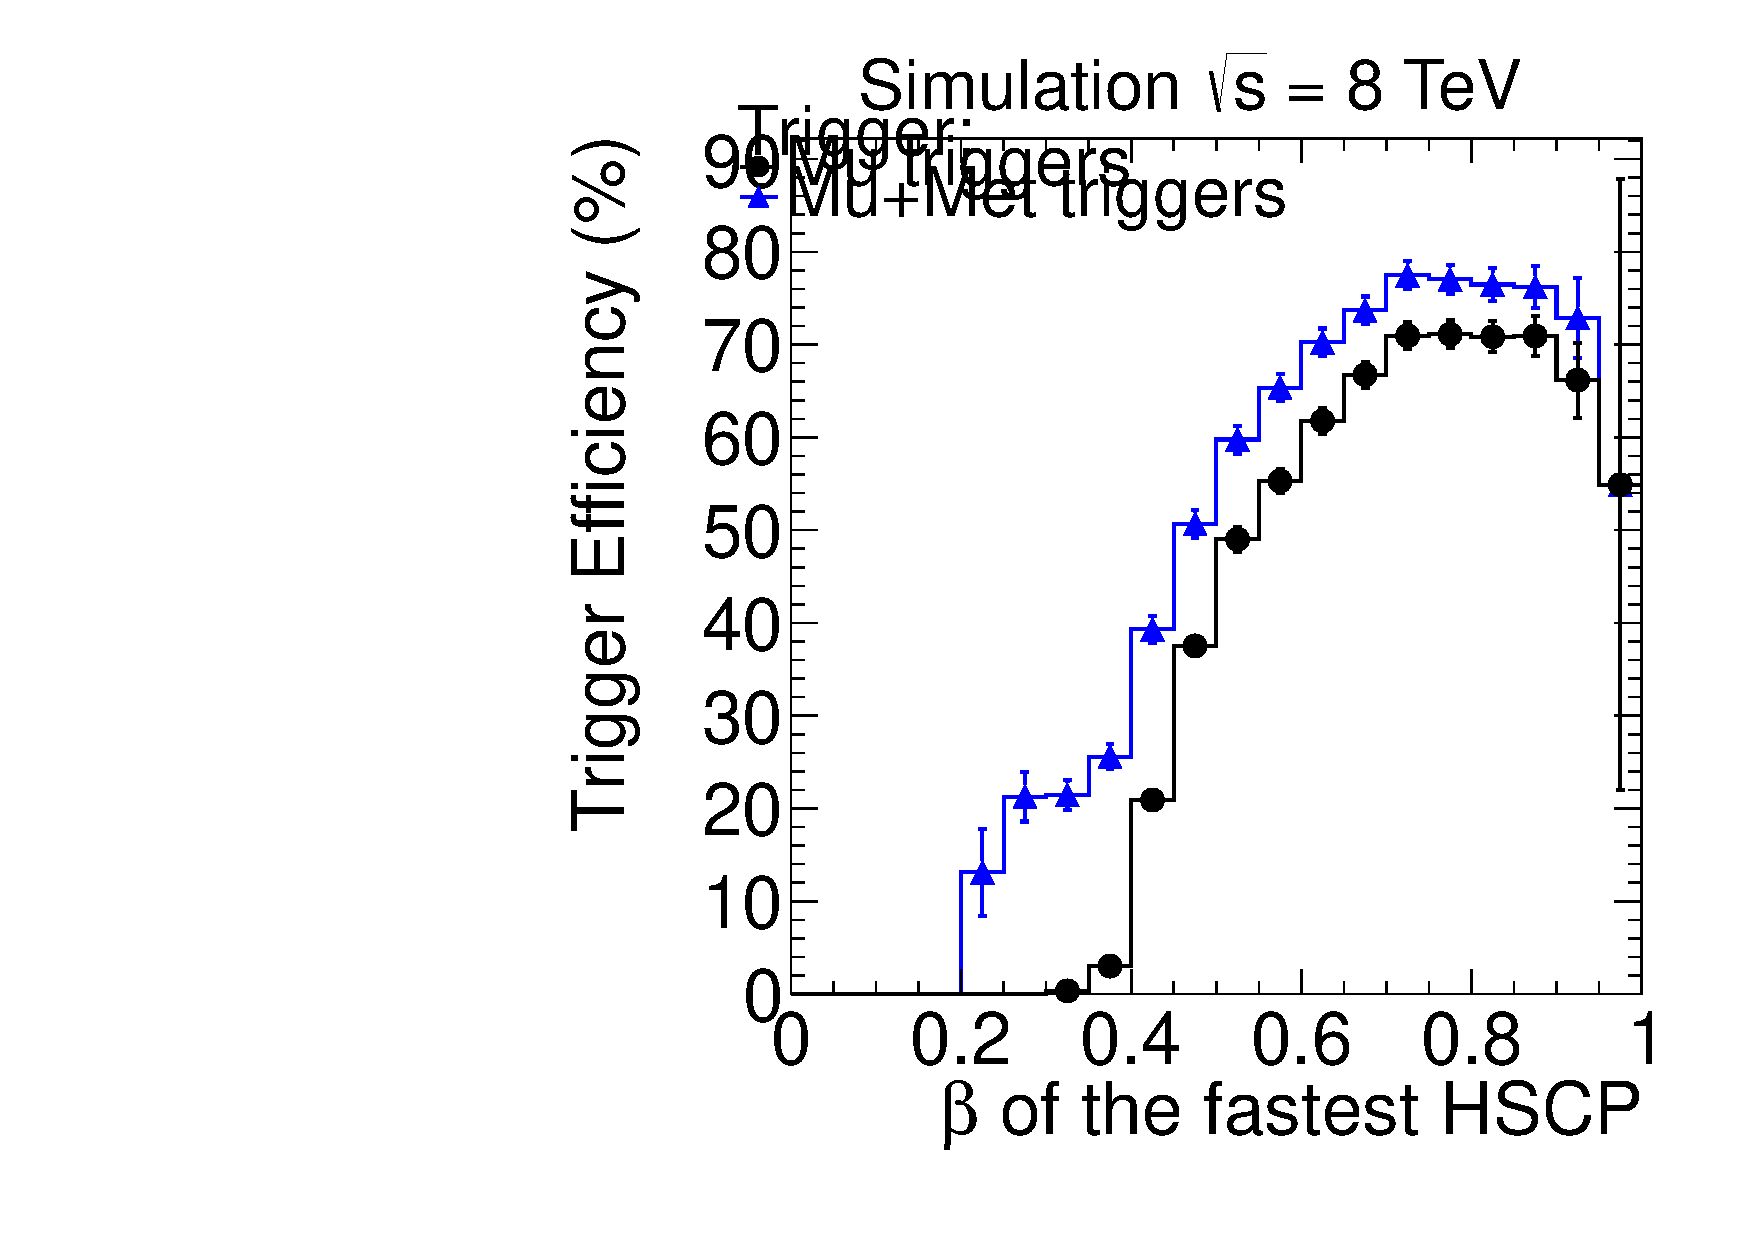
\includegraphics[clip=true, trim=0.0cm 0cm 3.0cm 0cm, width=0.32\textwidth]{figures/search/Stop_8TeV_M800MatchedGl}
  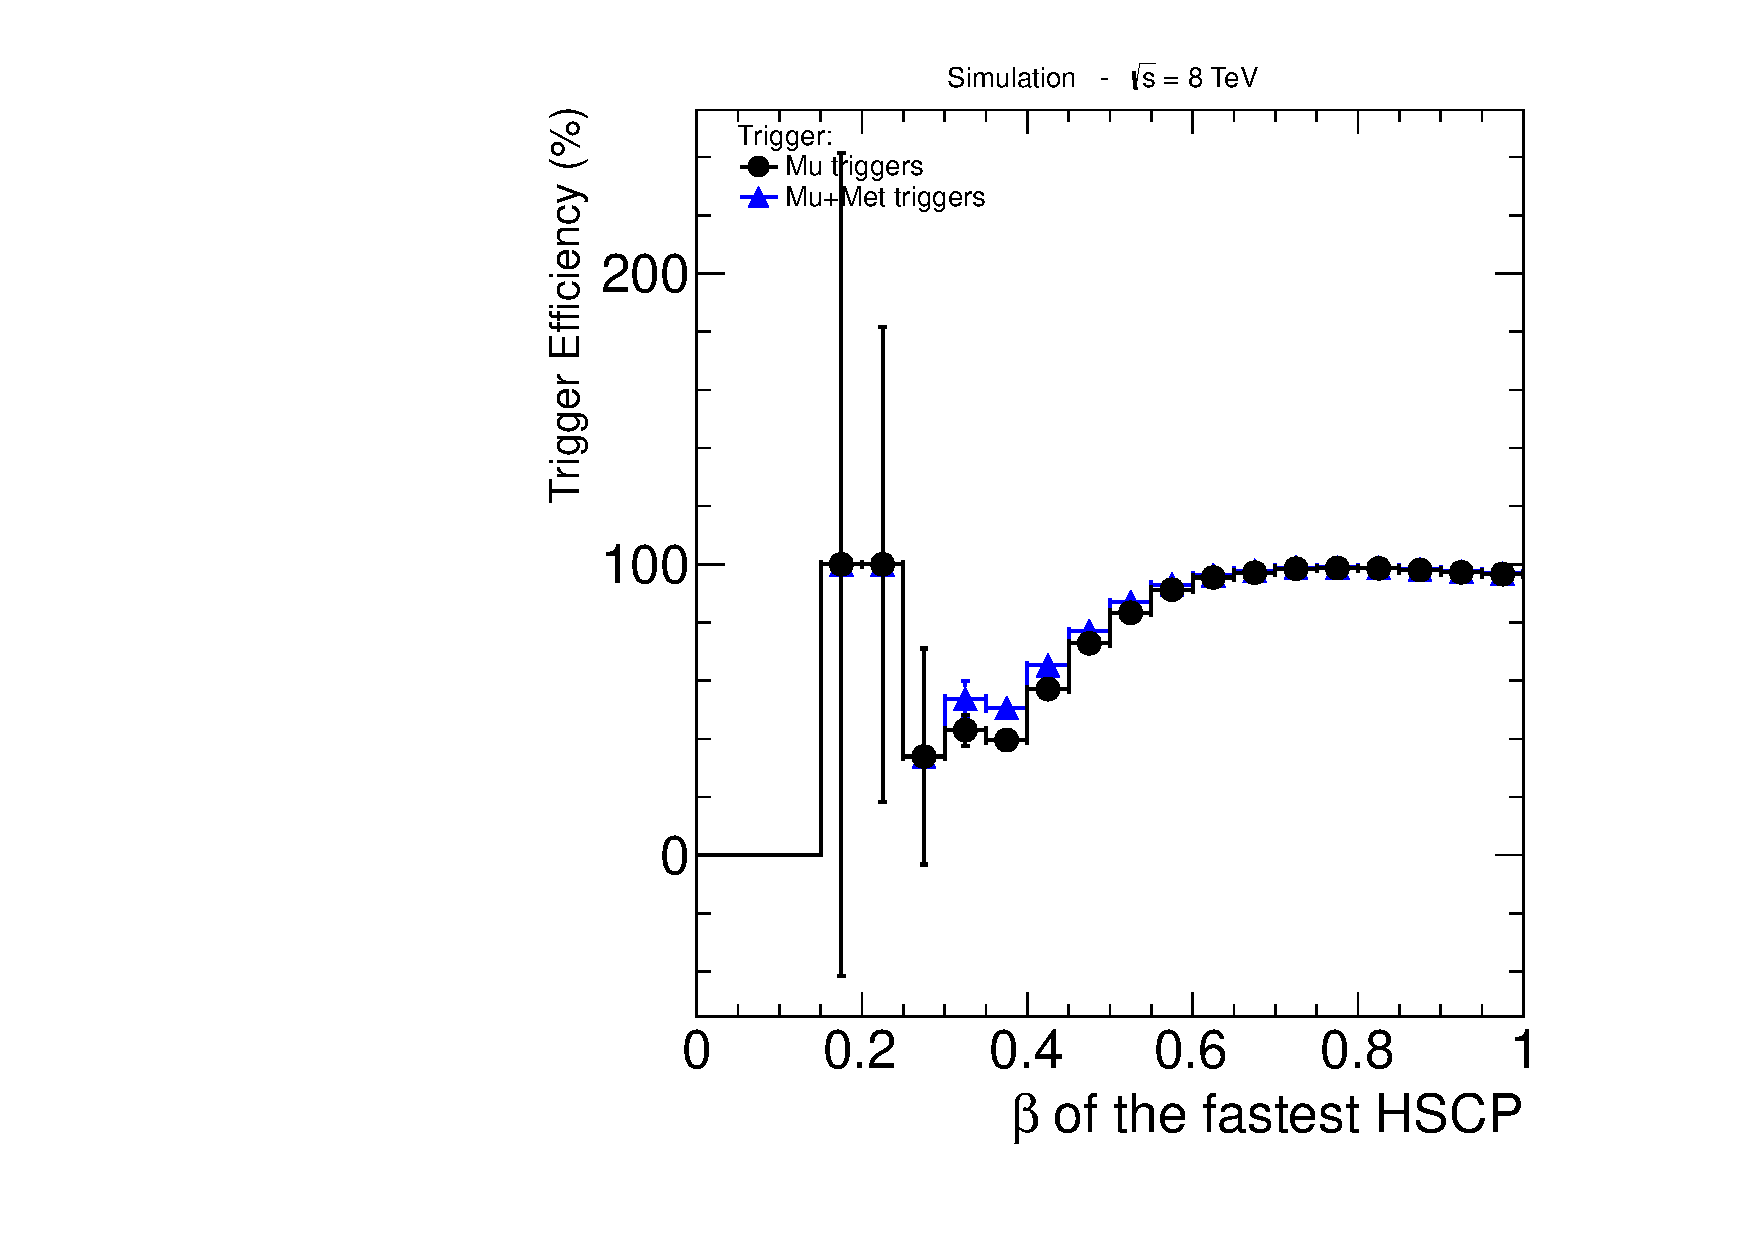
\includegraphics[clip=true, trim=0.0cm 0cm 3.0cm 0cm, width=0.32\textwidth]{figures/search/GMStau_8TeV_M494MatchedGl}
\caption{Trigger efficiency as a function of the $\beta$ of the fastest HSCP reconstructed in the event.
Top Row: Requiring reconstructed track be stand alone for 1200 GeV Gluino $f=1.0$ (left), 1200 GeV Gluino $f=0.1$ (middle), and 800 GeV Stop (right) samples.
Bottom Row: Requiring reconstructed track be global for 1200 GeV Gluino $f=0.1$ (left), 800 GeV Stop (middle), and 494 GeV GMSB Stau (right) samples.
    \label{fig:TriggerEffVsBetaGl}}
\end{figure}

The efficiency for each trigger as well as the combined efficiency is listed for various signals in Tables~\ref{tab:triggEffSA} and ~\ref{tab:triggEffGl} in events
with at least one HSCP reconstructed as a stand alone track and global track respectively.

\begin{table}
 \begin{center}
  \caption{Trigger efficiency for various models considered using the SingleMu, PFMET, L2Mu+MET or a combination of the three.
     \label{tab:triggEffSA}}
  \begin{tabular}{|l|c|c|c|c|c|} \hline
      Model     & Mass  & Mu40       & PFMET150   &  L2Mu+MET  & Total                 \\ \hline
 Gluino $f=0.1$ &  400  & 35.55      & 19.41      & 34.28      & 58.56    \\
 Gluino $f=0.1$ &  800  & 31.63      & 22.57      & 31.21      & 54.88    \\
 Gluino $f=0.1$ & 1200  & 26.62      & 20.45      & 24.63      & 47.52    \\
 Gluino $f=1.0$ &  400  &  5.55      & 23.22      & 36.63      & 46.07    \\
 Gluino $f=1.0$ &  800  &  5.01      & 24.50      & 31.88      & 43.41    \\
 Gluino $f=1.0$ & 1200  &  3.69      & 20.62      & 23.62      & 35.45    \\
           Stop &  200  & 42.79      & 11.15      & 27.31      & 58.80    \\
           Stop &  500  & 42.07      & 19.79      & 31.13      & 61.21    \\
           Stop &  800  & 41.57      & 21.57      & 30.33      & 60.73    \\ \hline
  \end{tabular}
 \end{center}
\end{table}

\begin{table}
 \begin{center}
  \caption{Trigger efficiency for various models considered using the SingleMu, PFMET, or a combination of the two.
     \label{tab:triggEffGl}}
  \begin{tabular}{|l|c|c|c|c|} \hline
      Model     & Mass  & Mu40       & PFMET150   & Total                 \\ \hline
 Gluino $f=0.1$ &  400  & 51.87      & 16.06      & 59.09    \\
 Gluino $f=0.1$ &  800  & 46.50      & 20.50      & 56.42    \\
 Gluino $f=0.1$ & 1200  & 38.96      & 19.56      & 49.95    \\
 Gluino $f=1.0$ &  400  & 41.81      & 19.36      & 51.76    \\
 Gluino $f=1.0$ &  800  & 37.83      & 21.57      & 49.01    \\
 Gluino $f=1.0$ & 1200  & 31.70      & 21.16      & 45.21    \\
           Stop &  200  & 58.43      &  7.69      & 61.54    \\
           Stop &  500  & 56.91      & 17.40      & 64.44    \\
           Stop &  800  & 56.15      & 20.49      & 65.59    \\
      GMSB Stau &  100  & 97.86      & 14.74      & 98.06    \\
      GMSB Stau &  308  & 97.03      & 17.53      & 97.47    \\
      GMSB Stau &  494  & 95.56      & 17.76      & 96.35    \\
        PP Stau &  100  & 95.06      &  0.17      & 95.09    \\
        PP Stau &  200  & 95.78      &  0.37      & 95.82    \\
        PP Stau &  494  & 95.23      &  1.16      & 95.36    \\ \hline
  \end{tabular}
 \end{center}
\end{table}

Muons from cosmic rays are an important background for the \muononly\ analysis. To study and predict them a trigger that selects events when no beams are passing through
CMS is used. The trigger requires the presence of a stand alone track with $p_T > 20$GeV, no coincidence with the LHC beams and for the event not to be flagged as
beam halo. The stand alone track reconstruction used for the cosmic trigger is slightly different than for the collision trigger as it is not updated at vertex, the
meaning of this is discussed in section~\ref{sec:preselection}. However offline both reconstructions are required so no bias is introduced.

\section{Selection Variables}
The low velocity of the HSCP leads to two interesting detector signatures. The first is that the particles will arrive at the detector elements later than SM particles would.
The muon system, being the furthest detector element from the interaction point, has the largest timing difference. The measurement of the arrival time of particles in the
muon system is discussed in section~\ref{sec:timing}.

The second signature is that a slow moving HSCP will have a larger ionization energy loss in the silicon tracker than SM particles will.
The dependence of the ionization energy lost on velocity is described by the Bethe-Bloch formula~\cite{PDG}. SM particles with momentum 10-1000 GeV all deposit
roughly the same amount of energy per unit length, $\dedx,$ ($\approx$ 3MeV/cm) and are often referred to as minimum ionizing particles (MIPs).
For particles with $0.1 < \beta < 1$ \dedx\ varies as $\sim 1/\beta^2$.
As in~\cite{2012PAS} three variables related to \dedx\ are calculated for each track. The first is \ih which is an estimator of the \dedx\ of the track.
The second is \ias\ which is a discrimant that checks the probability that a MIP would produce a charge less than or equal to the charge of each of the hits
along the track. The discrimant peaks at zero for MIPs and approaches one for high-ionizing particles. The last is \iasp\ which has the same form as \ias\ except
the probability is that a MIP would produce a charge more than or equal to the charge of the hits, this variable is only used in the fractionally charged analysis.

An estimate of the mass, assuming Q=1e, of a particle can be made from \ih\ and the momentum of a track. This is done by using Eq.~\ref{eq:MassFromHarmonicEstimator},
also from Ref.~\cite{2011HSCP},

\begin{equation}
I_h= K\cfrac{m^2}{p^2}+C.
\label{eq:MassFromHarmonicEstimator}
\end{equation}

with  $K=2.559 \pm 0.001$ MeV cm$^{-1}$ $c^2$ and
$C=2.772 \pm 0.001$ MeV cm$^{-1}$.

As HSCP would be created by BSM theories at high energies they are likely to have high momentum. For this reason the $p_T$ of the track is used as a third
selection variable. 

The \tktof\ measurement uses the $p_T$ measurement coming from the inner tracker while the \muononly\ analysis uses the measurement from the muon system.
The HSCP is likely to stay the same charge while
passing through the inner tracker so the \tktof\ is relatively unaffected by this. However for the $p_T$ measurement from the muon system it can result in the $p_T$ of the
HSCP to be overestimated.

CMS measures the curvature of a track which is function of the $q/p_T$ of the track. A charge of $|q|=1e$ is assumed in order to determine the $p_T$ of the track.
For HSCP that can modify their charge inside of CMS it can be the case that the average value of q during its passage through the muon system does not equal one.
This effect has different consequences for the stop and gluino samples. A stop particle,
specifically not an anti-stop, has a charge of $+(2/3)e$ and forms a $R$-hadron with either an anti-quark ($\tilde{t} \bar{q}$) or
two quarks  ($\tilde{t} q q$). Anti-quarks have a charge of $-(2/3)e$ or $+(1/3)e$ leading to $R$-hadrons with a charge
of either 0 or $+1e$. Quarks have a charge of either $+(2/3)e$ or $-(1/3)e$ which allows for
the creation of $R$-hadrons with a charge of 0, $+1e$, or $+2e$. Thus a stop $R$-hadron will always have a
positive charge or be neutral. For an anti-stop, the effect is reversed and the $R$-hadron will always have a
negative charge or be neutral.

For gluino particles this statement does not hold true. Gluinos can hadronize in gluon balls ($\tilde{g}g$), $R$-mesons ($\tilde{g} q \bar{q}$), or
$R$-baryons ($\tilde{g} qqq$ or $\tilde{g} \bar{q}\bar{q}\bar{q}$), with either quarks or
anti-quarks allowing the charge of the $R$-hadron to range from $-2e$ to $+2e$. This leads to the
average charge of the $R$-hadron as it traverses the muon system to be less than $1e$ and the $p_T$
value to be overestimated.

To observe this effect the function
$\Delta(q/p_T)$ is defined in Equation~\ref{eq:deltaqopt}

\begin{equation}
\Delta(q/p_T) = ((q/p_T)_{SA} - (q/p_T)_{Inner})/(q/p_T)_{Inner}
\label{eq:deltaqopt}
\end{equation}

where SA refers to stand alone track qualities and Inner refers to
inner track qualities.
Figure~\ref{fig:MuOnlyInvPtDiff} shows the distribution of
$\Delta(q/p_T)$ for tracks with inner track $p_T > 200$ GeV
for data and various HSCP signal samples.
A value of zero in this plot indicates the $p_T$ was reconstructed correctly
while negative one indicates the reconstructed $p_T$ approaches infinity.
The GMSB stau sample, which does not change charge,
has a distribution similar to data, though slightly wider.
The stop sample, which are not able to flip charge but merely to switch
between one sign and zero, is centered at zero but with a slightly wider
width than data or GMSB stau.
The gluino samples, which can flip charge, are centered at negative one meaning that
their reconstructed $p_T$ is normally larger than what is generated, sometimes
to a very large degree.  This effect causes further discrimination of gluino HSCP
from background Standard Model particles.

\begin{figure}
 \begin{center}
  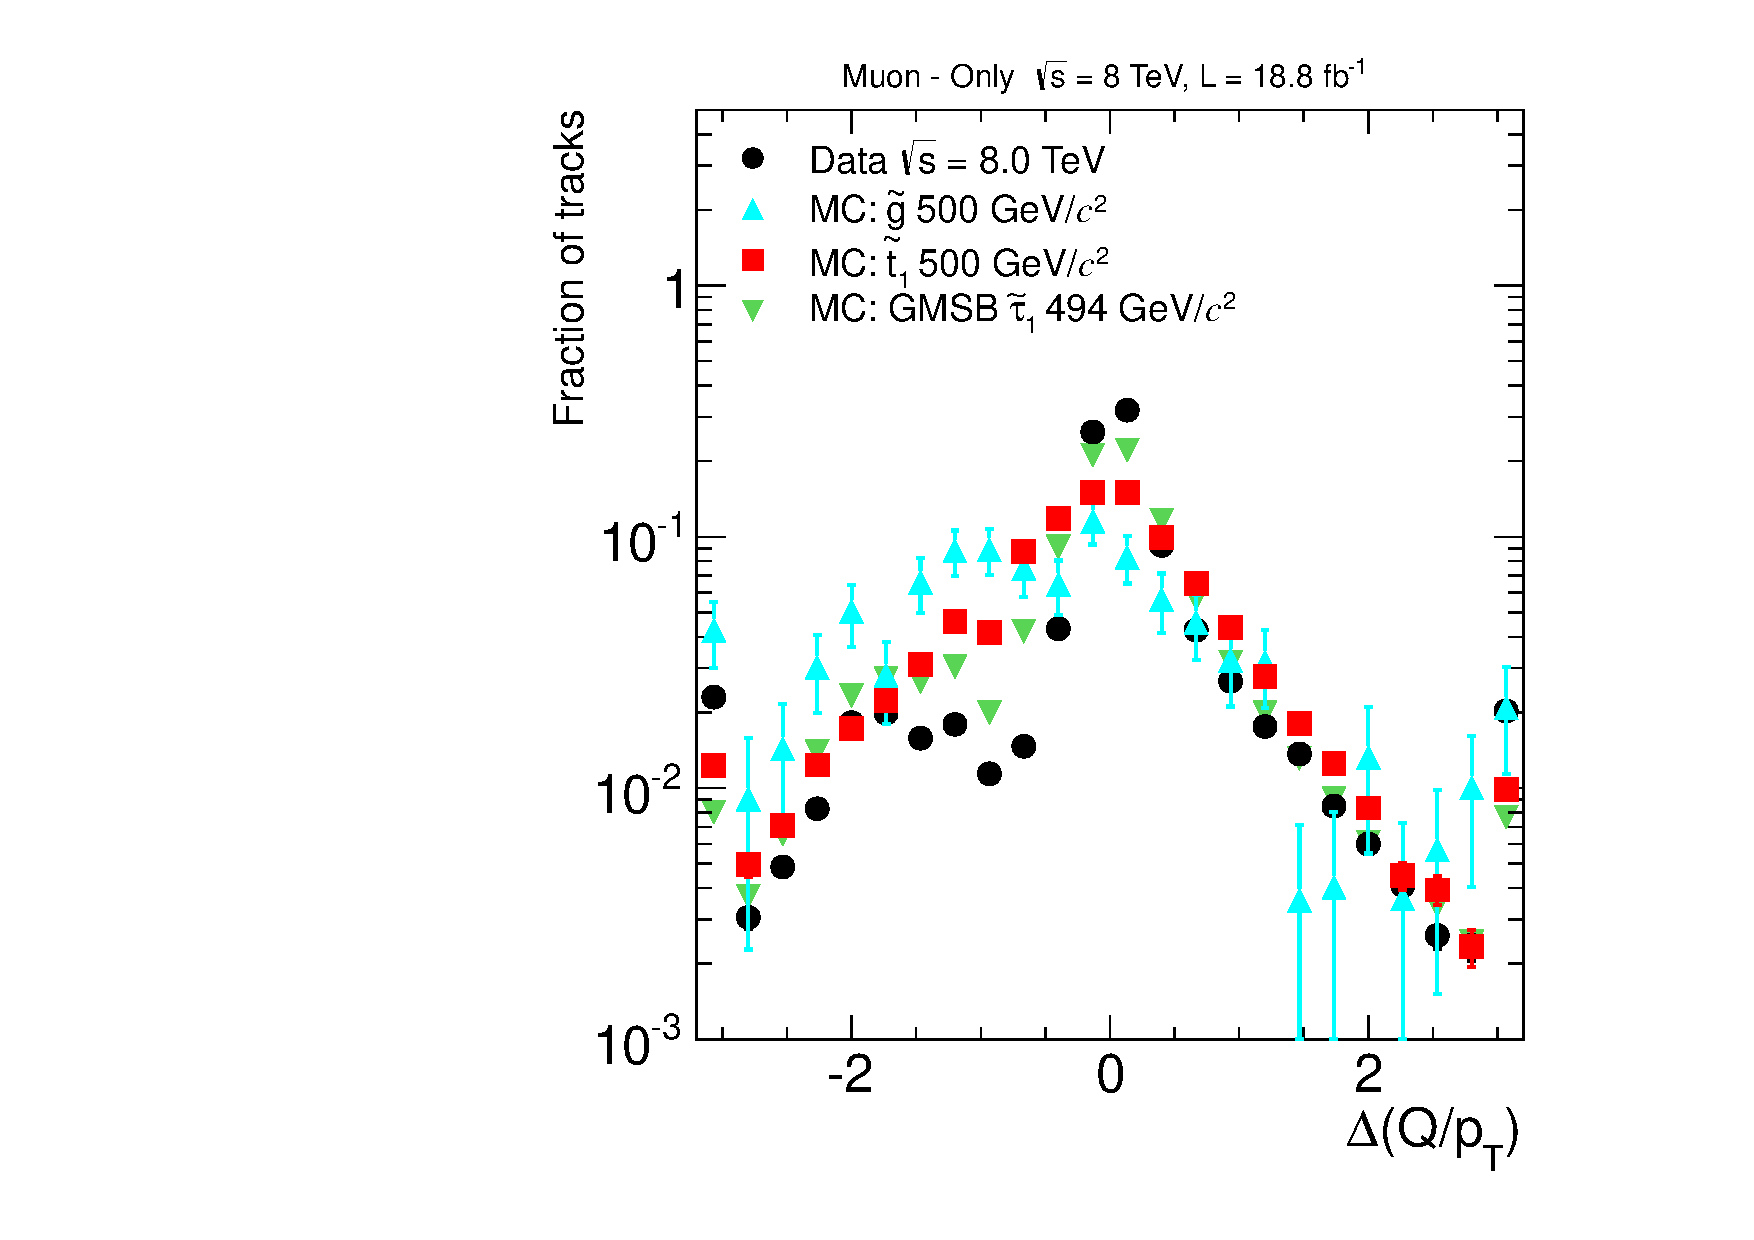
\includegraphics[width=0.44\textwidth]{figures/muonly/Selection_Comp_Signal_8TeV_InnerInvPtDiff_BS}
 \end{center}
 \caption{Distribution of $\Delta(q/p_T)$
    for data, 500 GeV gluino, 500 GeV stop, and 494 GeV
    GMSB stau.
    \label{fig:MuOnlyInvPtDiff}}
\end{figure}

For the lepton like samples with non-unit charge the \pt\ will be mismeasured by a factor of 1/Q, meaning fractionally charged particles will have their \pt\ overestimated
while multiply charged particles will be underestimated. This effect can be seen in Figure~\ref{fig:RecoGenPt}.

\begin{figure}
 \begin{center}
  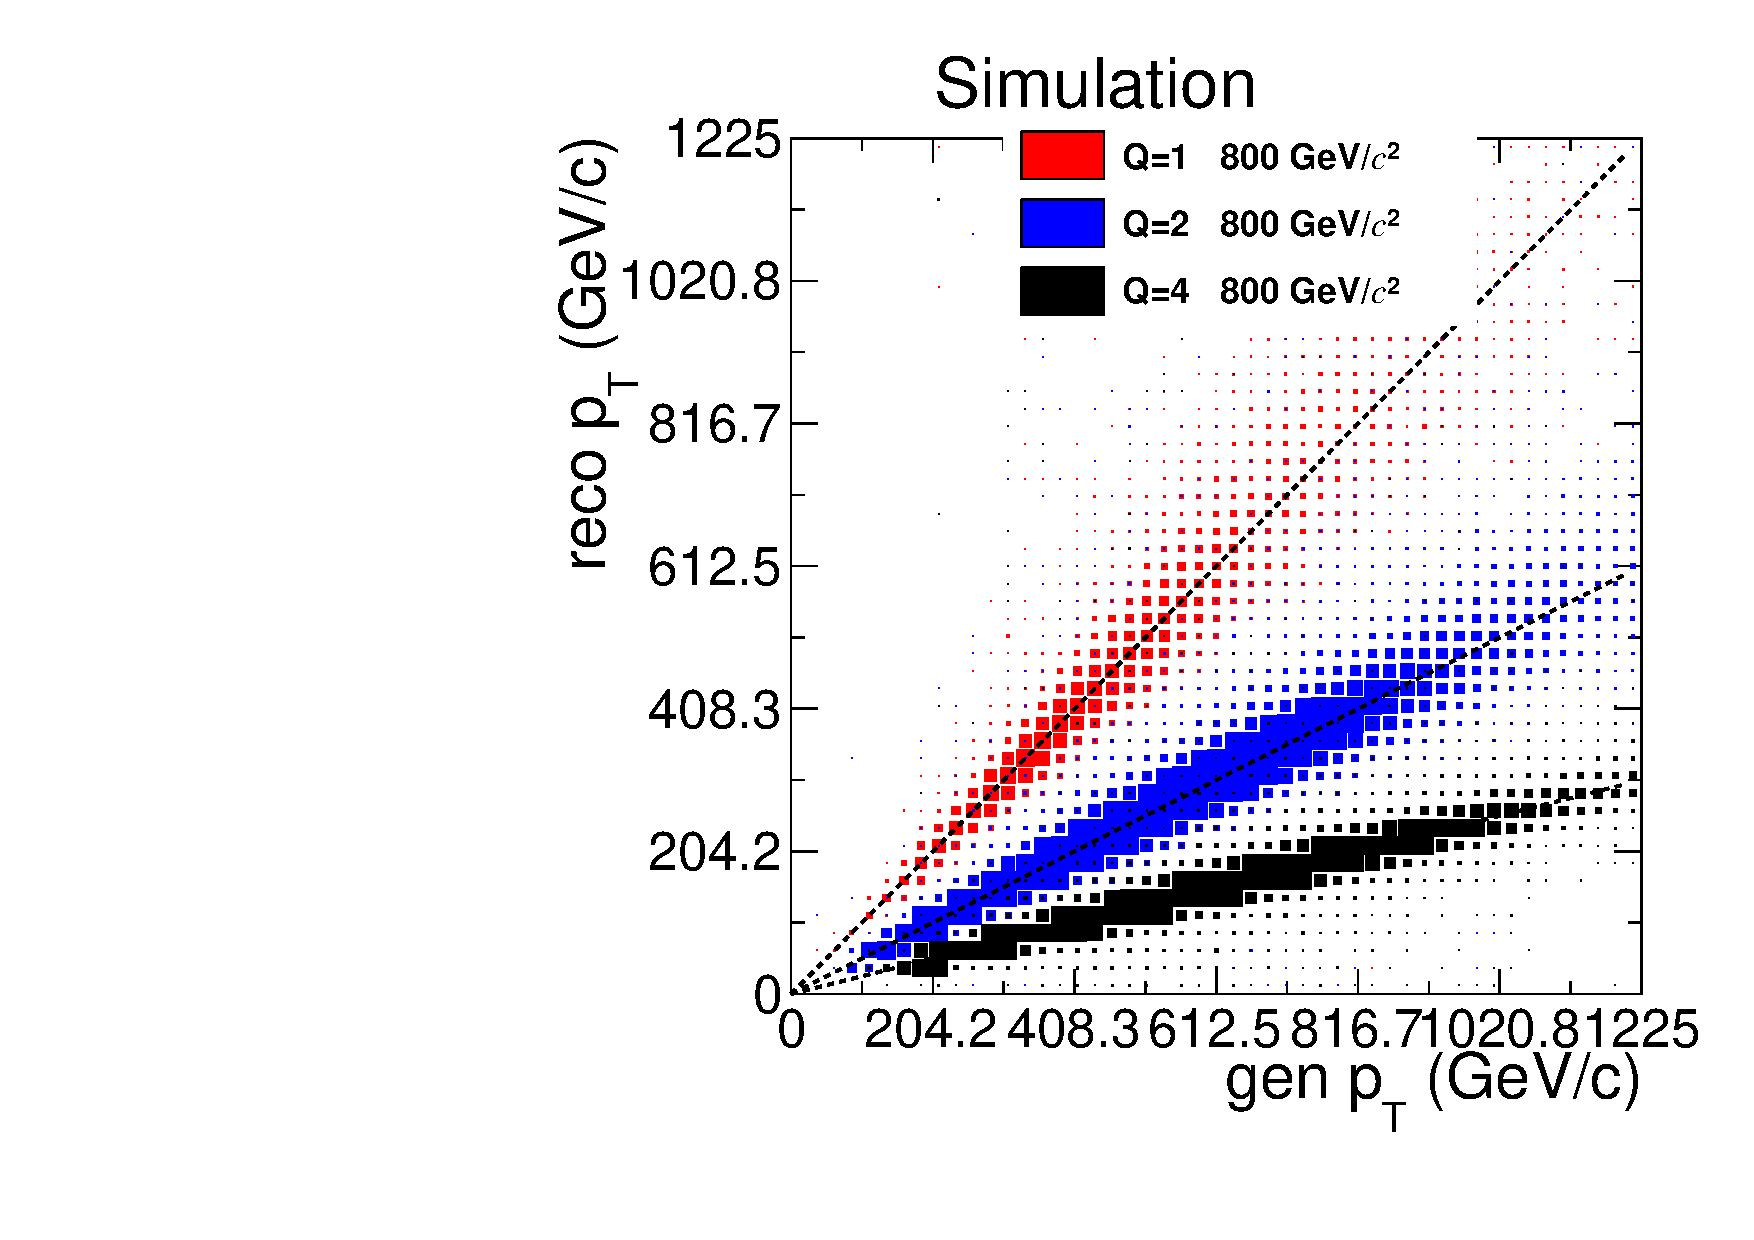
\includegraphics[width=0.44\textwidth]{figures/tkonly/SIM_Validation_Pt.pdf}
 \end{center}
 \caption{Distribution of reconstructed $p_T$ versus generator $p_T$ for Q=2e/3, 1e, and 2e samples.
    \label{fig:RecoGenPt}}
\end{figure}

\section{Preselection \label{sec:preselection}}
Candidates for the \muononly\ analysis are tracks reconstructed in the muon system. Candidates for the \tktof\ and \multi\ analysis are tracks found in both the muon
system and the inner tracker. The \tkonly and fract\ analyses require only that the tracks be found in the inner tracker.
Various requirements are applied to the candidate in order to reduce tracks from background process while maintaining good efficiency for HSCP.

The \muononly\ analysis requires the candidates to have $p_T > 80$, $|\eta| < 2.1$, and valid DT or CSC hits in at least two muon stations
to reinforce the requirements applied at trigger level. Quality cuts on the
\invbeta\ measurement are applied. The measurement must have at least eight degrees of freedom and the error must be less than 0.07.
A potential background source is muons coming from
out of time bunch crossings. Candidates are required to have a measured time leaving the vertex not be within 5ns of an out of time bunch crossing.
Figure~\ref{fig:MuOnlyPreselA} shows the distribution of these quantities for data, cosmic control sample, and signal MC.
Additional cuts are used to control the background from cosmic rays. The displacement of the track
with respect to the beam spot is required to be less than 15cm in both the longitudinal and transverse direction relative to the beam line. 
The candidate $|\phi|$ must not be within 1.2--1.9, this region represents tracks pointing in the vertical
direction, as is expected of cosmic rays. Cosmic rays travel through the top and bottom halves of the detector leaving hits in the muon system opposite of the candidate.
It is required that  there be no muon segments with $\eta$ within 0.1 of $-\eta_{candidate}$. Only segments separated from the candidate by at least 0.5 in $\phi$
are used to prevent candidates in the central portion of the detector to match to their own segments.
Figure~\ref{fig:MuOnlyPreselB} shows the distribution of these quantities.

\begin{figure}
\centering
  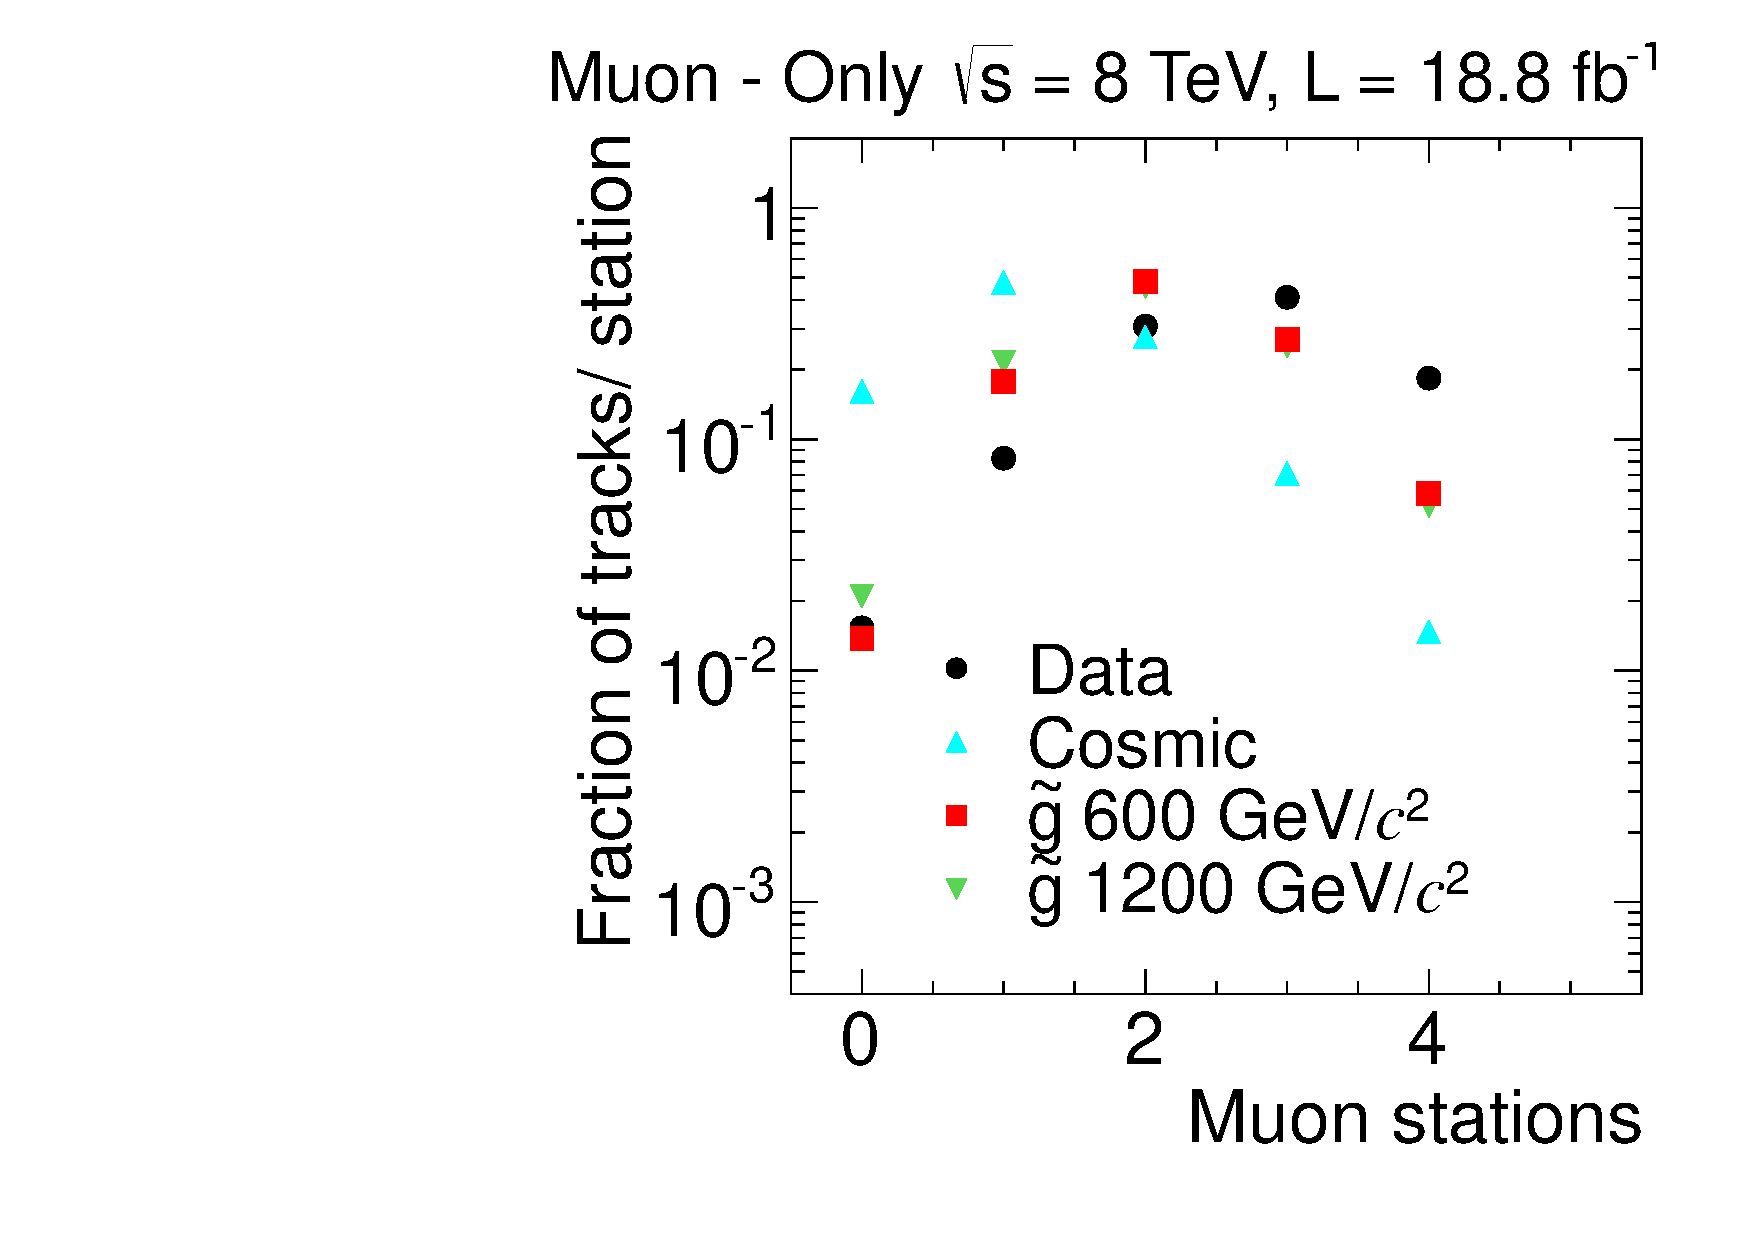
\includegraphics[clip=true, trim=0.0cm 0cm 2.8cm 0cm, width=0.44\textwidth]{figures/muonly/Selection_Comp_8TeV_Cosmic_MatchedStations_BS}
  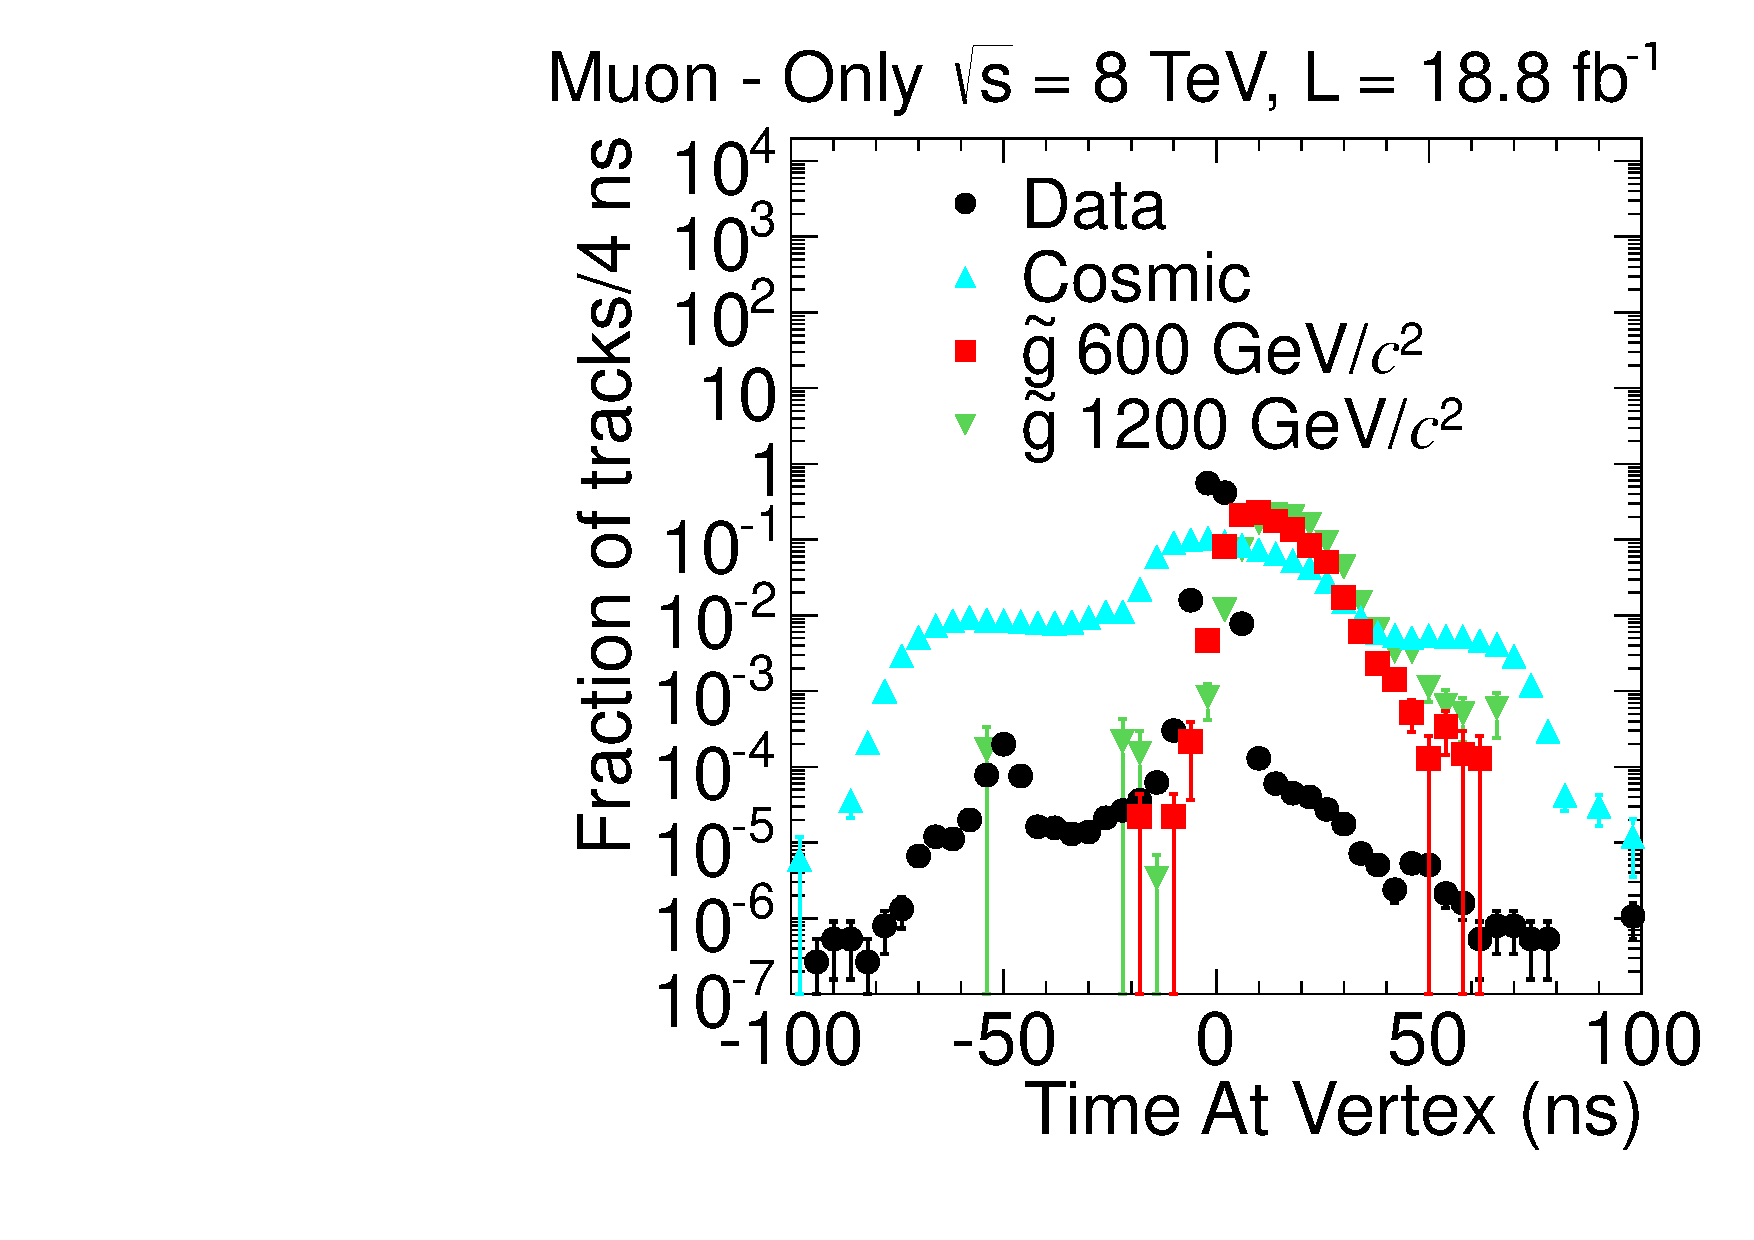
\includegraphics[clip=true, trim=0.0cm 0cm 2.8cm 0cm, width=0.44\textwidth]{figures/muonly/Selection_Comp_8TeV_Cosmic_TimeAtIP_BS} \\
  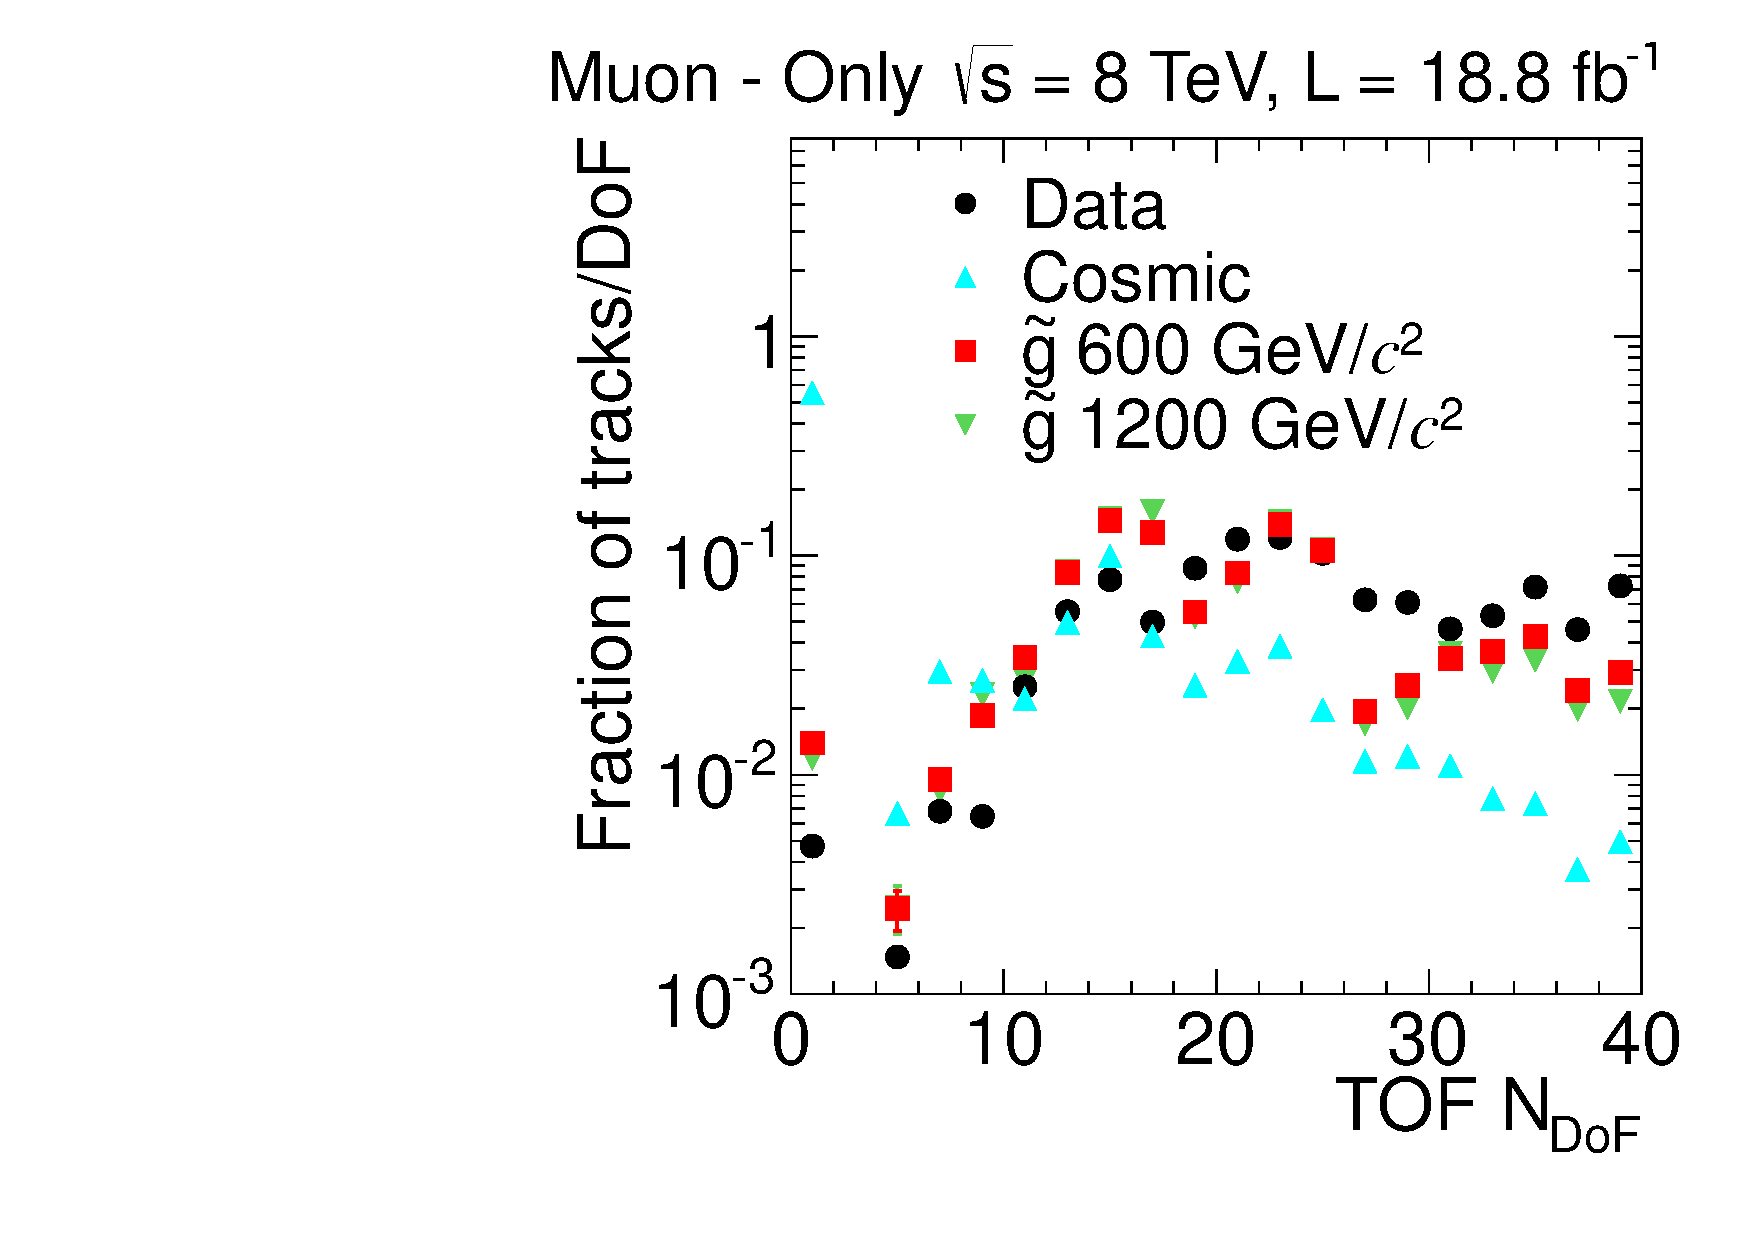
\includegraphics[clip=true, trim=0.0cm 0cm 2.8cm 0cm, width=0.44\textwidth]{figures/muonly/Selection_Comp_8TeV_Cosmic_nDof_BS}
  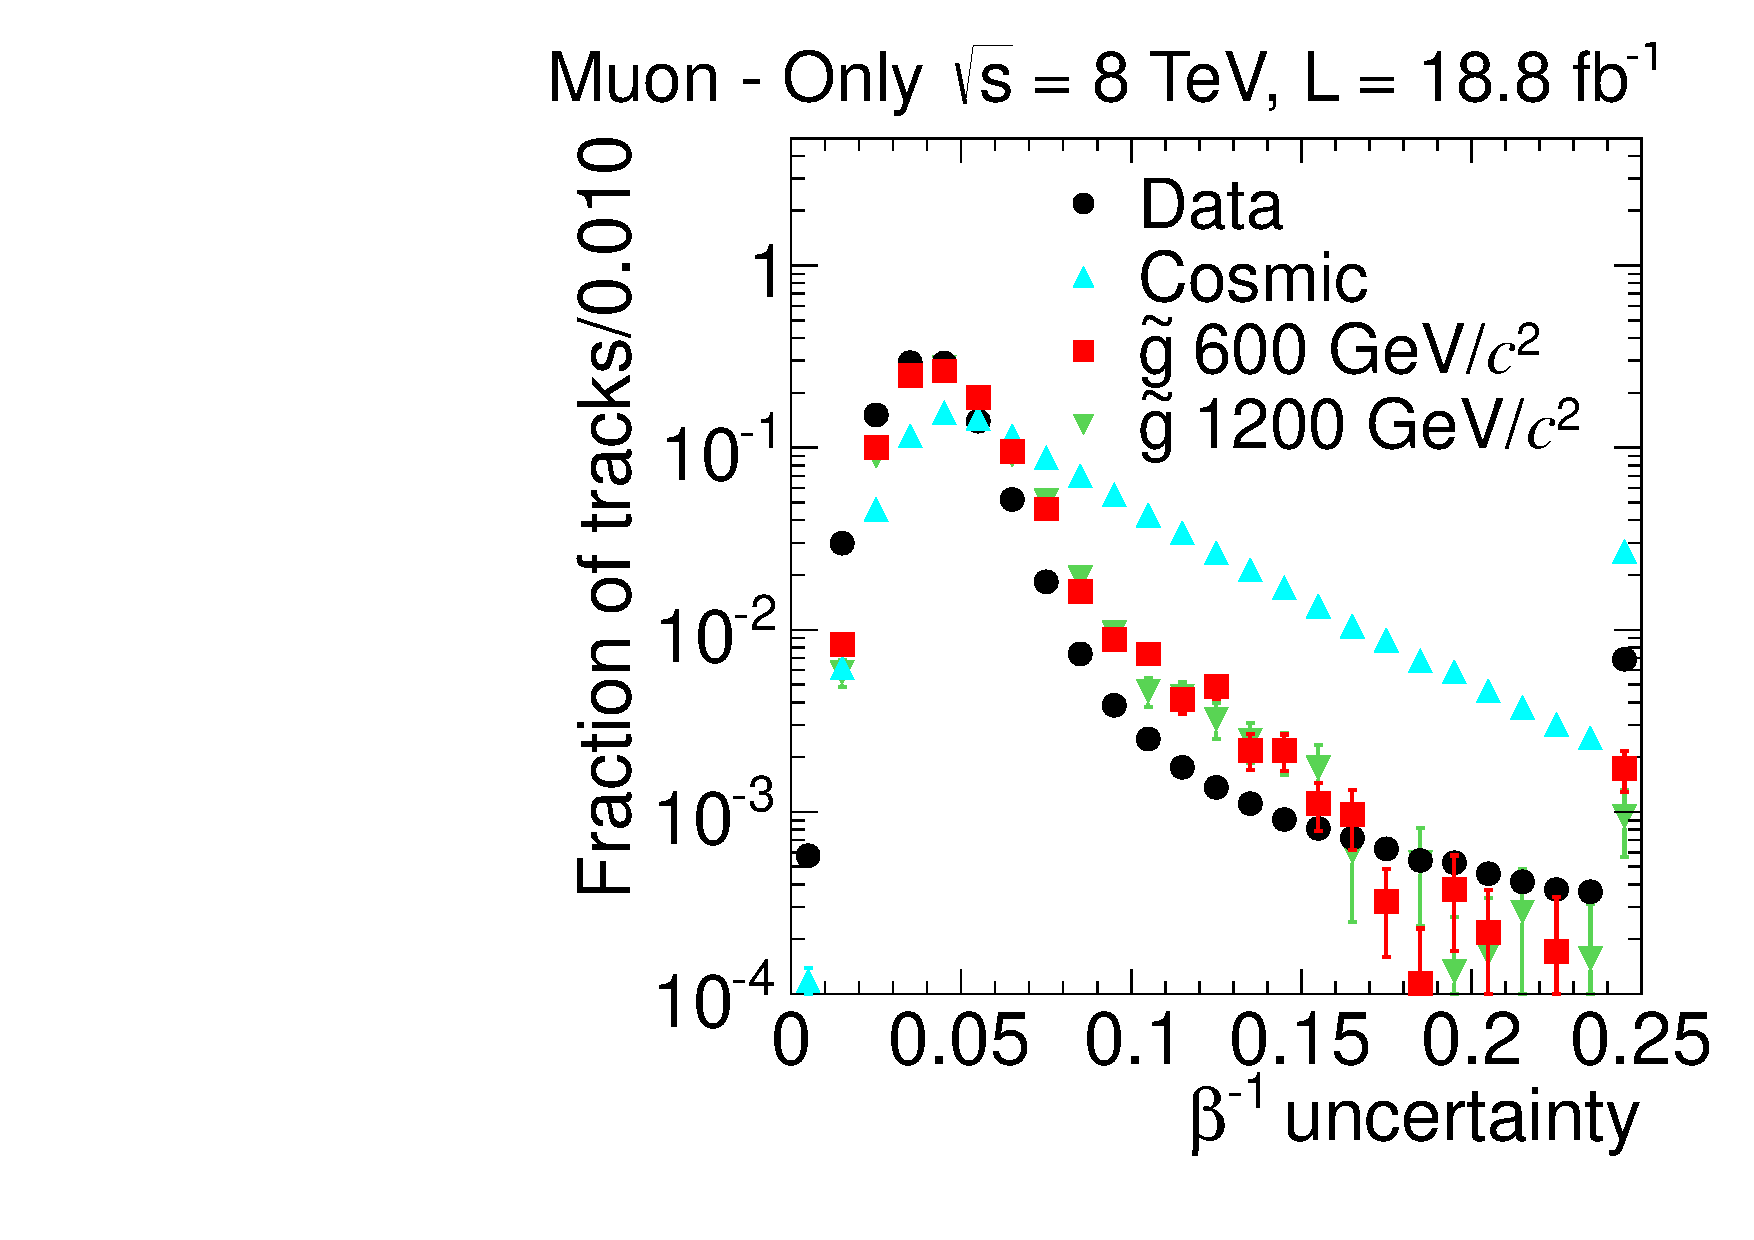
\includegraphics[clip=true, trim=0.0cm 0cm 2.8cm 0cm, width=0.44\textwidth]{figures/muonly/Selection_Comp_8TeV_Cosmic_TOFError_BS}
\caption{Distribution of various prelection variables for data, cosmic control sample, and signal MC.
Top row: Disitribution of number of matched stations (left) and time at vertex (right).
Bottom row:Number of degrees of freedom (left) and error (right) on \invbeta\ measurement.
    \label{fig:MuOnlyPreselA}}
\end{figure}

\begin{figure}
\centering
  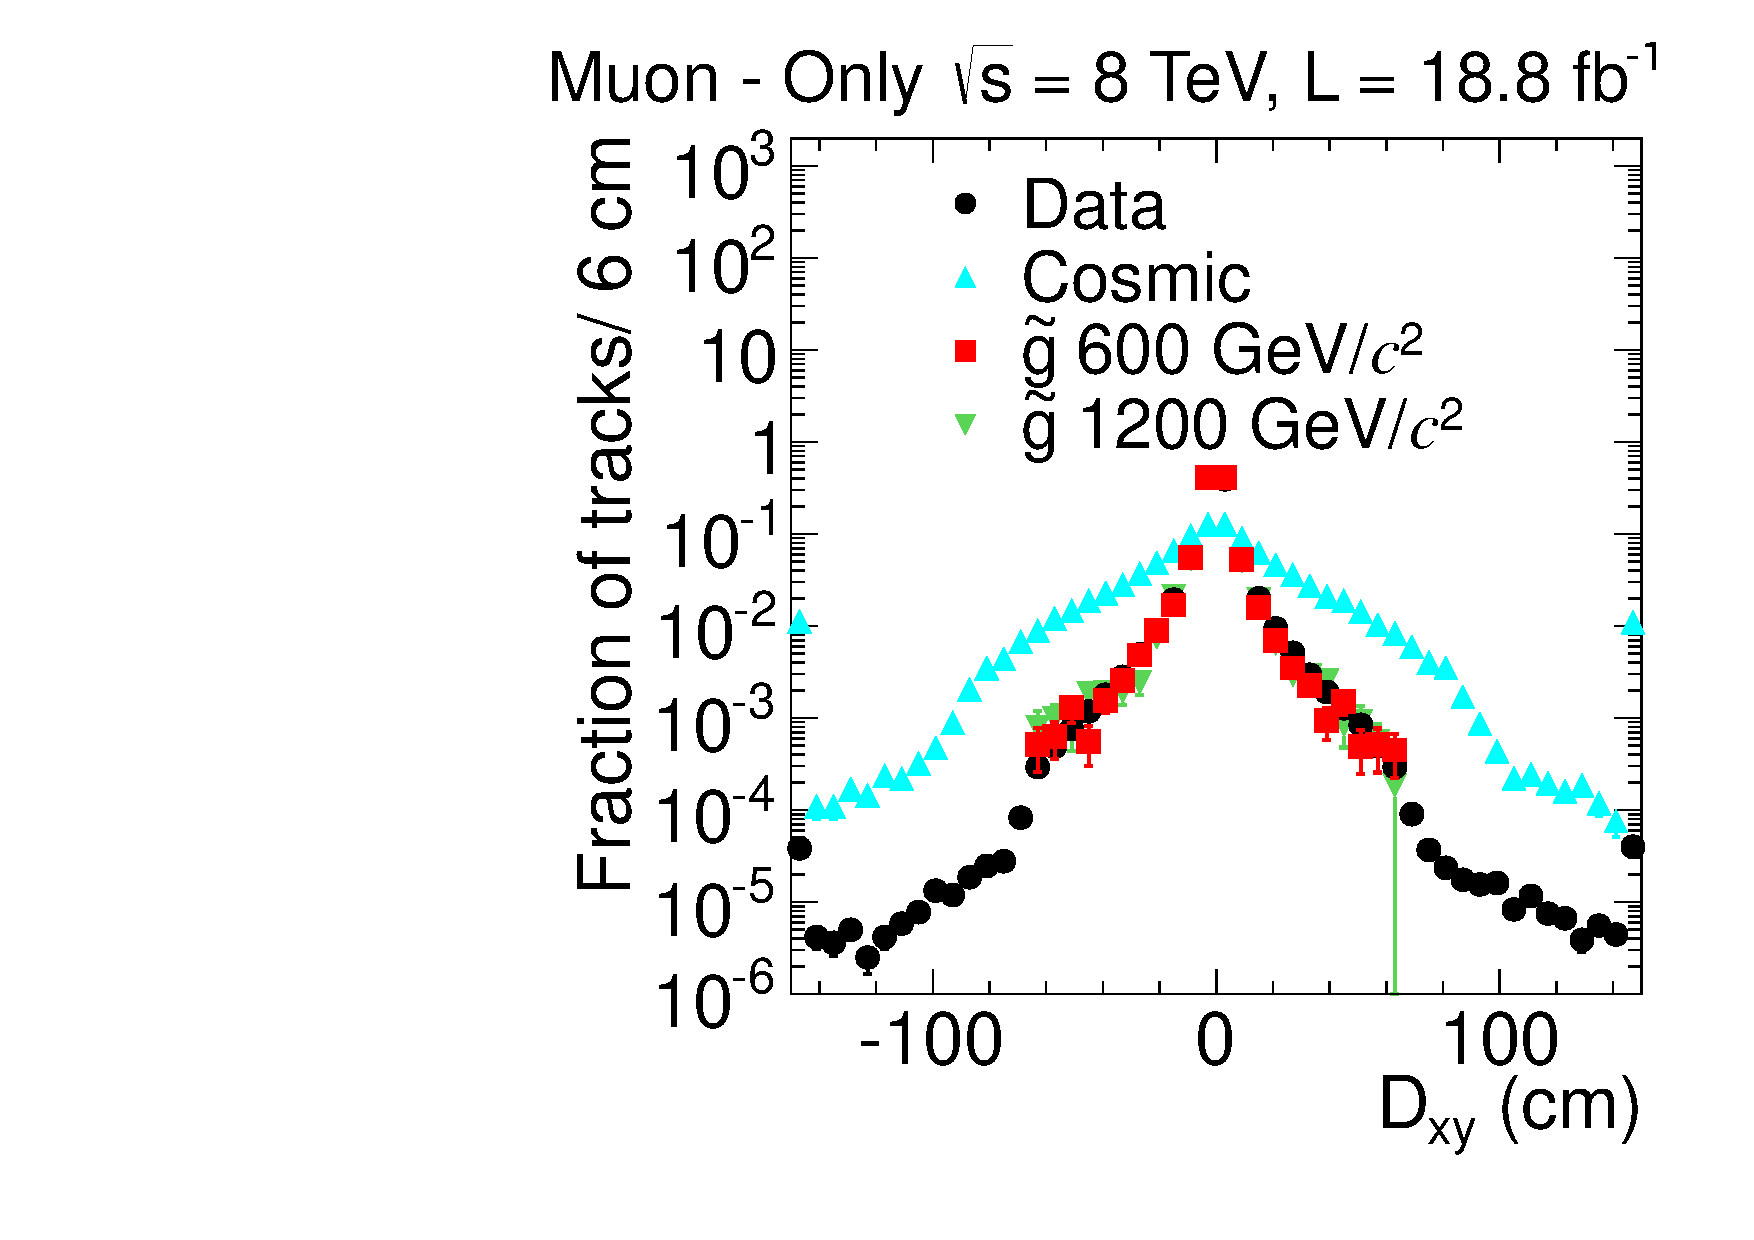
\includegraphics[clip=true, trim=0.0cm 0cm 2.8cm 0cm, width=0.44\textwidth]{figures/muonly/Selection_Comp_8TeV_Cosmic_Dxy_BS}
  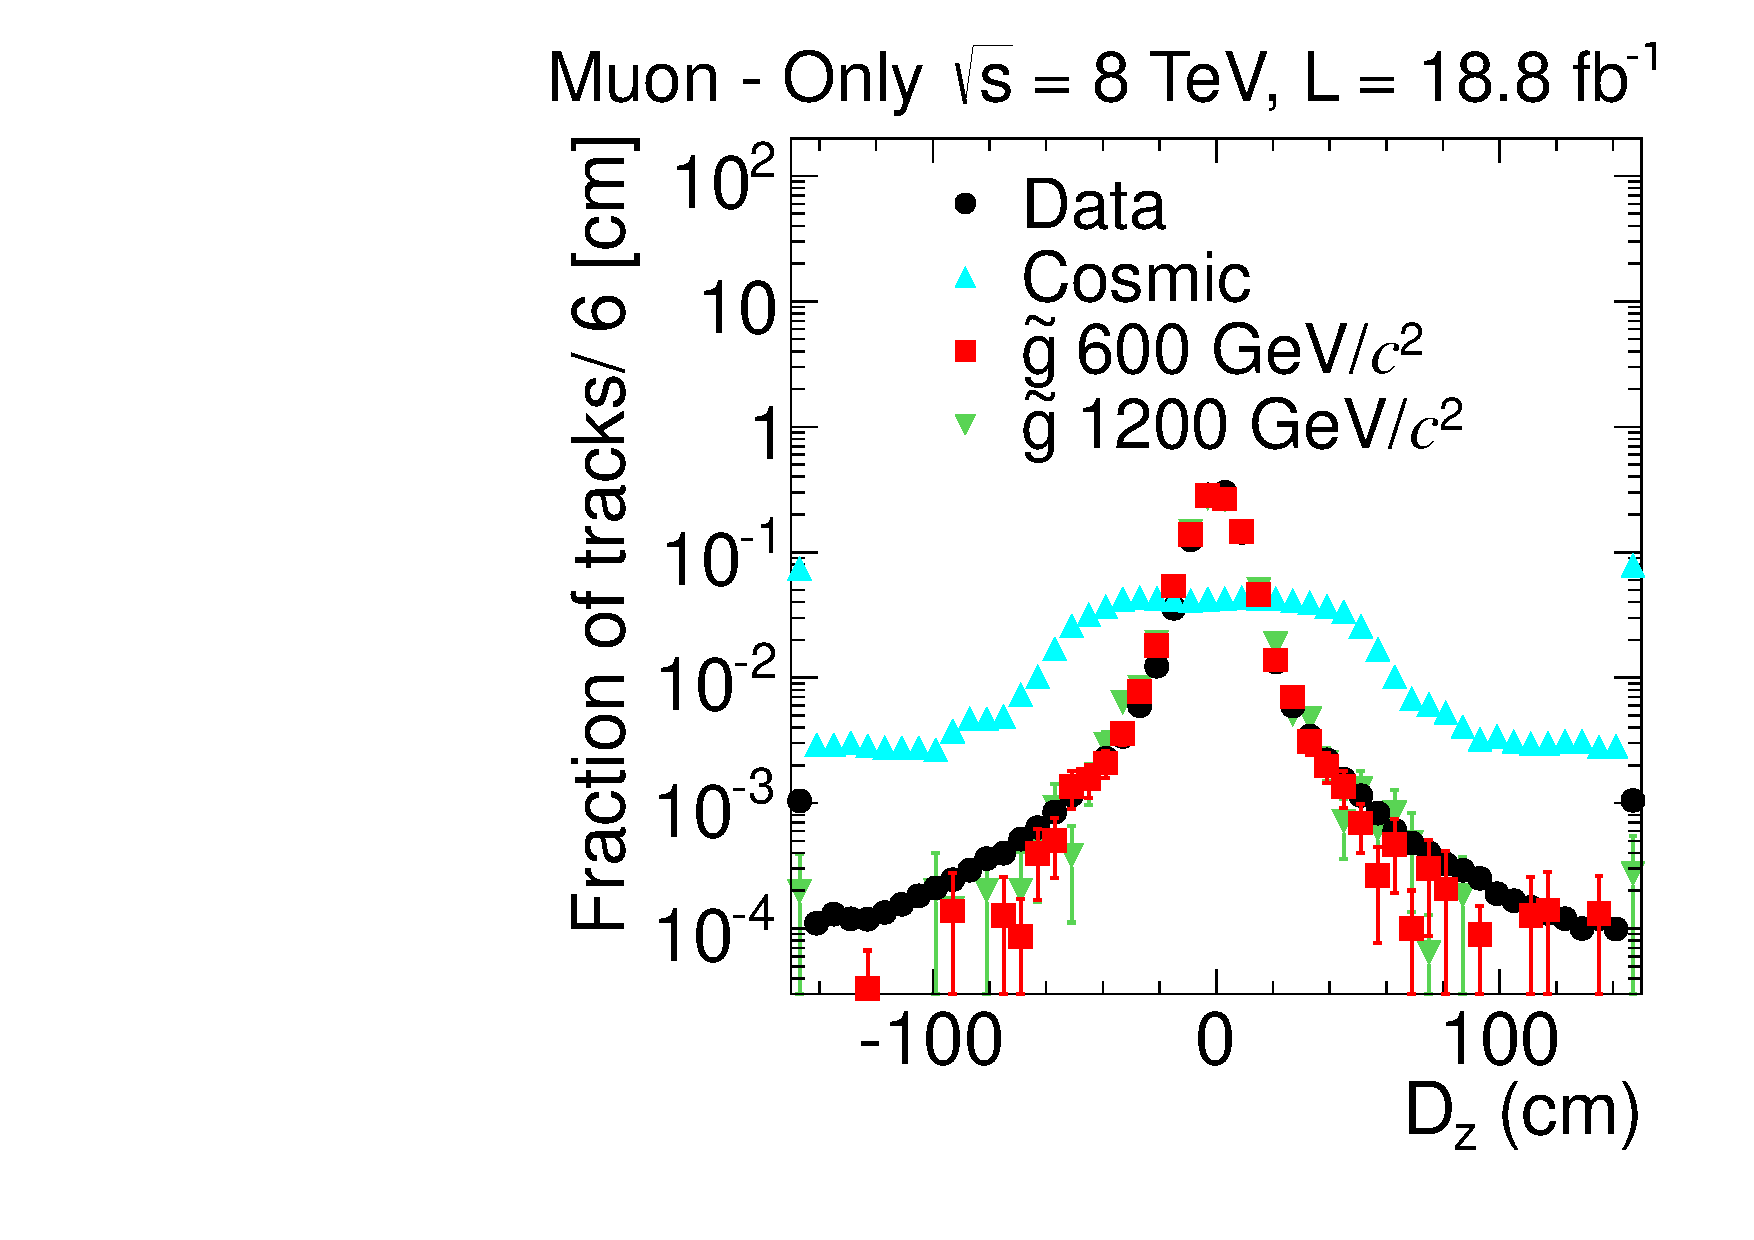
\includegraphics[clip=true, trim=0.0cm 0cm 2.8cm 0cm, width=0.44\textwidth]{figures/muonly/Selection_Comp_8TeV_Cosmic_Dz_BS} \\
  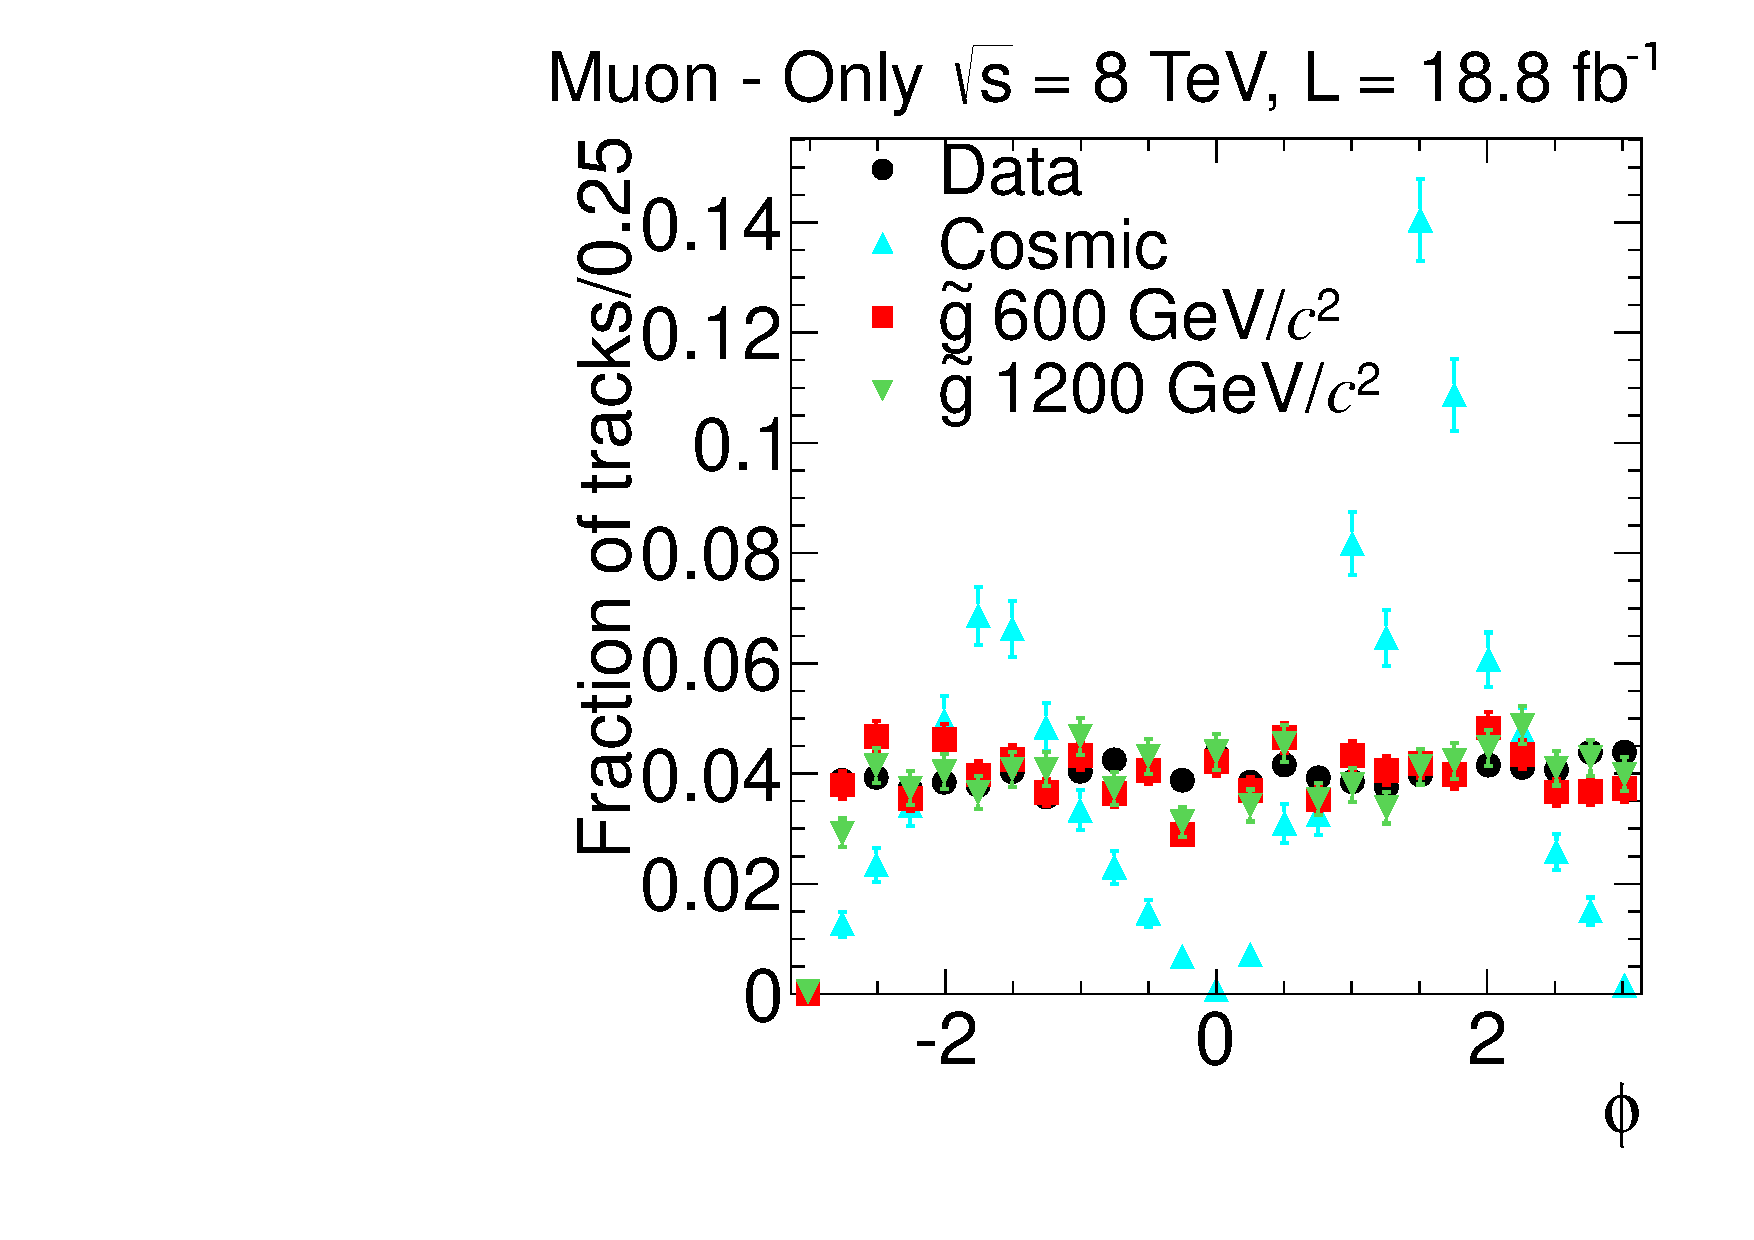
\includegraphics[clip=true, trim=0.0cm 0cm 2.8cm 0cm, width=0.44\textwidth]{figures/muonly/Selection_Comp_8TeV_Cosmic_Phi_BS}
  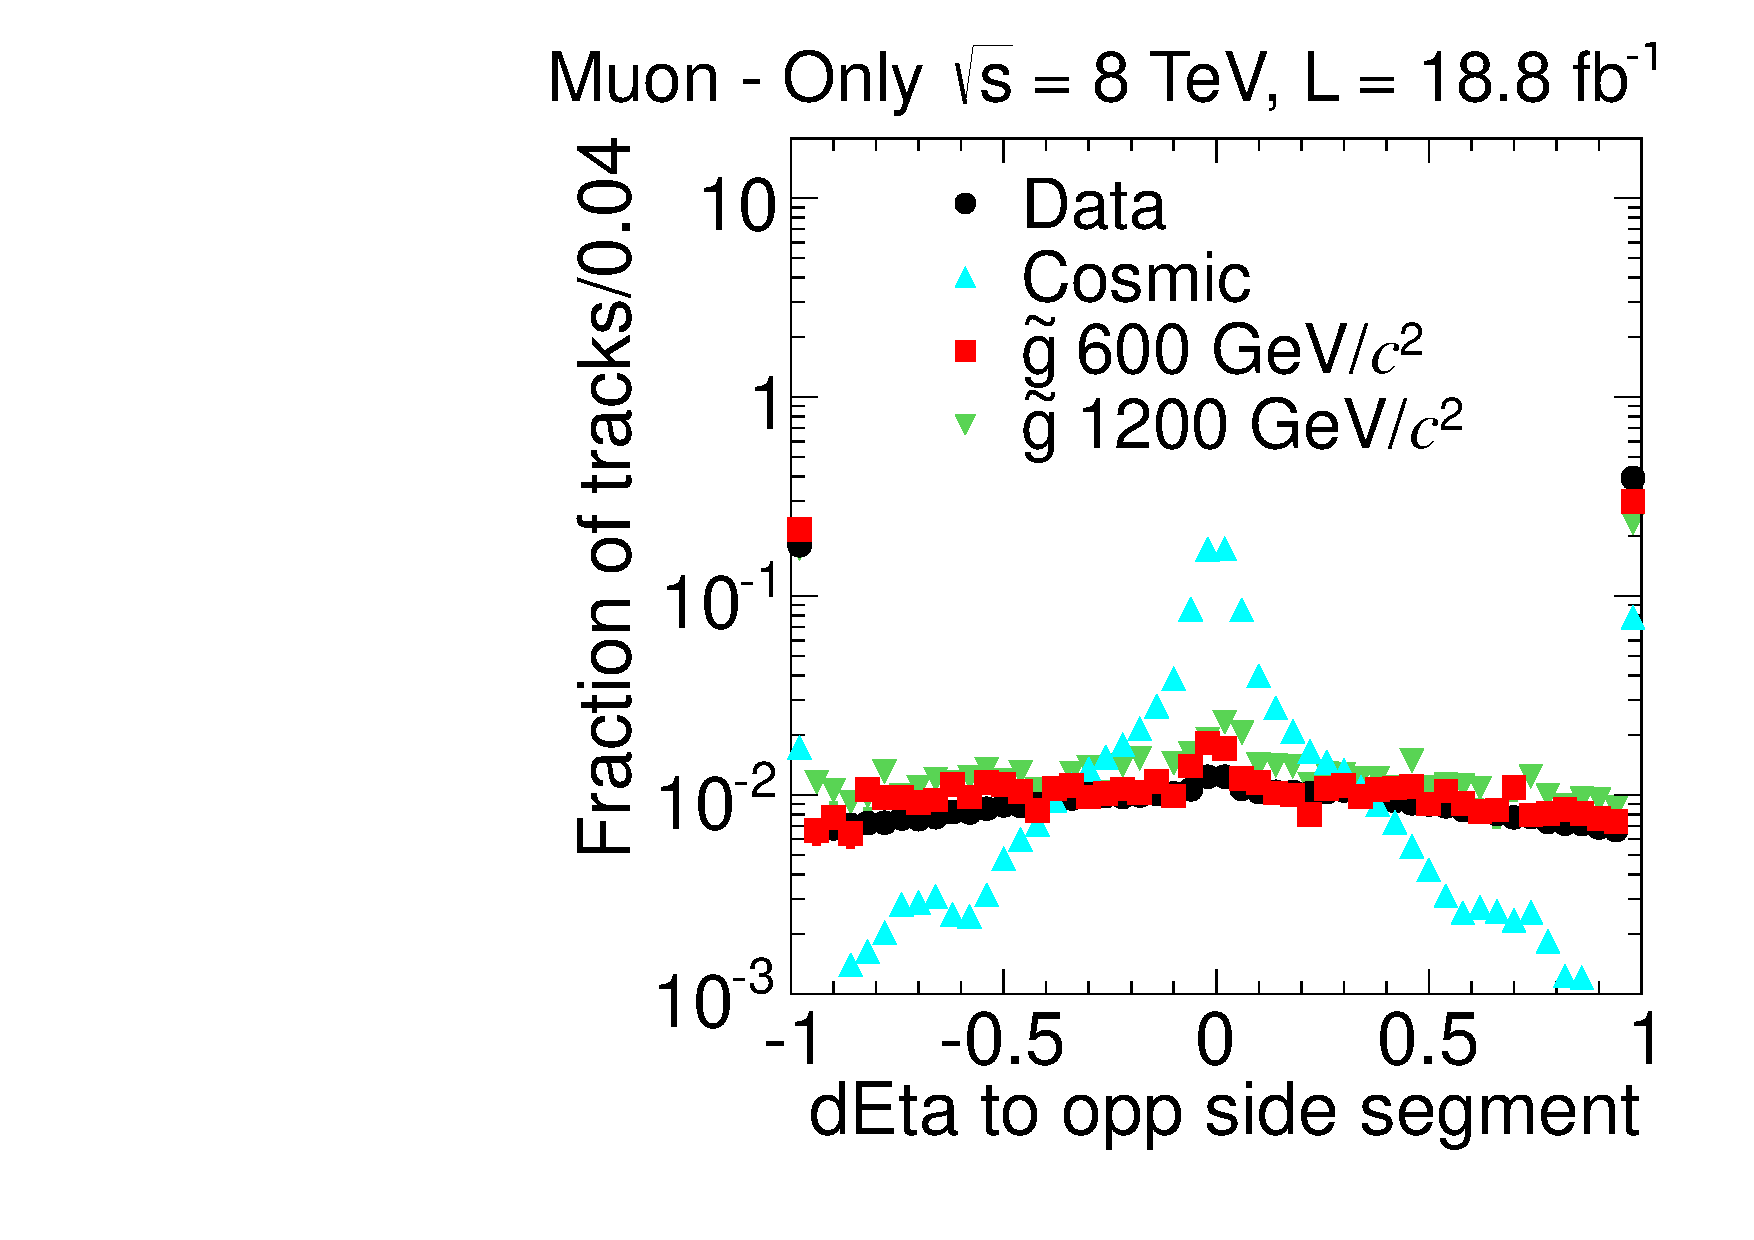
\includegraphics[clip=true, trim=0.0cm 0cm 2.8cm 0cm, width=0.44\textwidth]{figures/muonly/Selection_Comp_8TeV_Cosmic_SegMinEtaSep_BS}
  \caption{Distribution of various prelection variables for data, cosmic control sample, and signal MC.
Top row: Disitribution of transverse (left) and longitudinal displacement (right).
Bottom row: Distribution of $\phi$ (left) and $\eta$ separation to muon segments (right).
    \label{fig:MuOnlyPreselB}}
\end{figure}

The \tktof\ analysis applies cuts on the inner tracker track which has a much better $p_T$ and impact parameter resolution than the muon system track.
The candidate is required to have $p_T > 45$ and  $|\eta| < 2.1$ to match the trigger level requirements. 
Quality cuts are applied as low quality background tracks can have mismeasured moment and potentially high fluctuations in \dedx.
The inner track is required to have at least eight hits in the inner tracker with at least two coming from the pixel detector. At least 80\% of the hits associated with the track
must be considered valid. A cleaning procedure is applied to the hits before calculating \dedx\ and there must be at least six measurements passing this cleaning.
Figure~\ref{fig:TkMuPreselA} shows these variables for data and signal MC.

\begin{figure}
\centering
  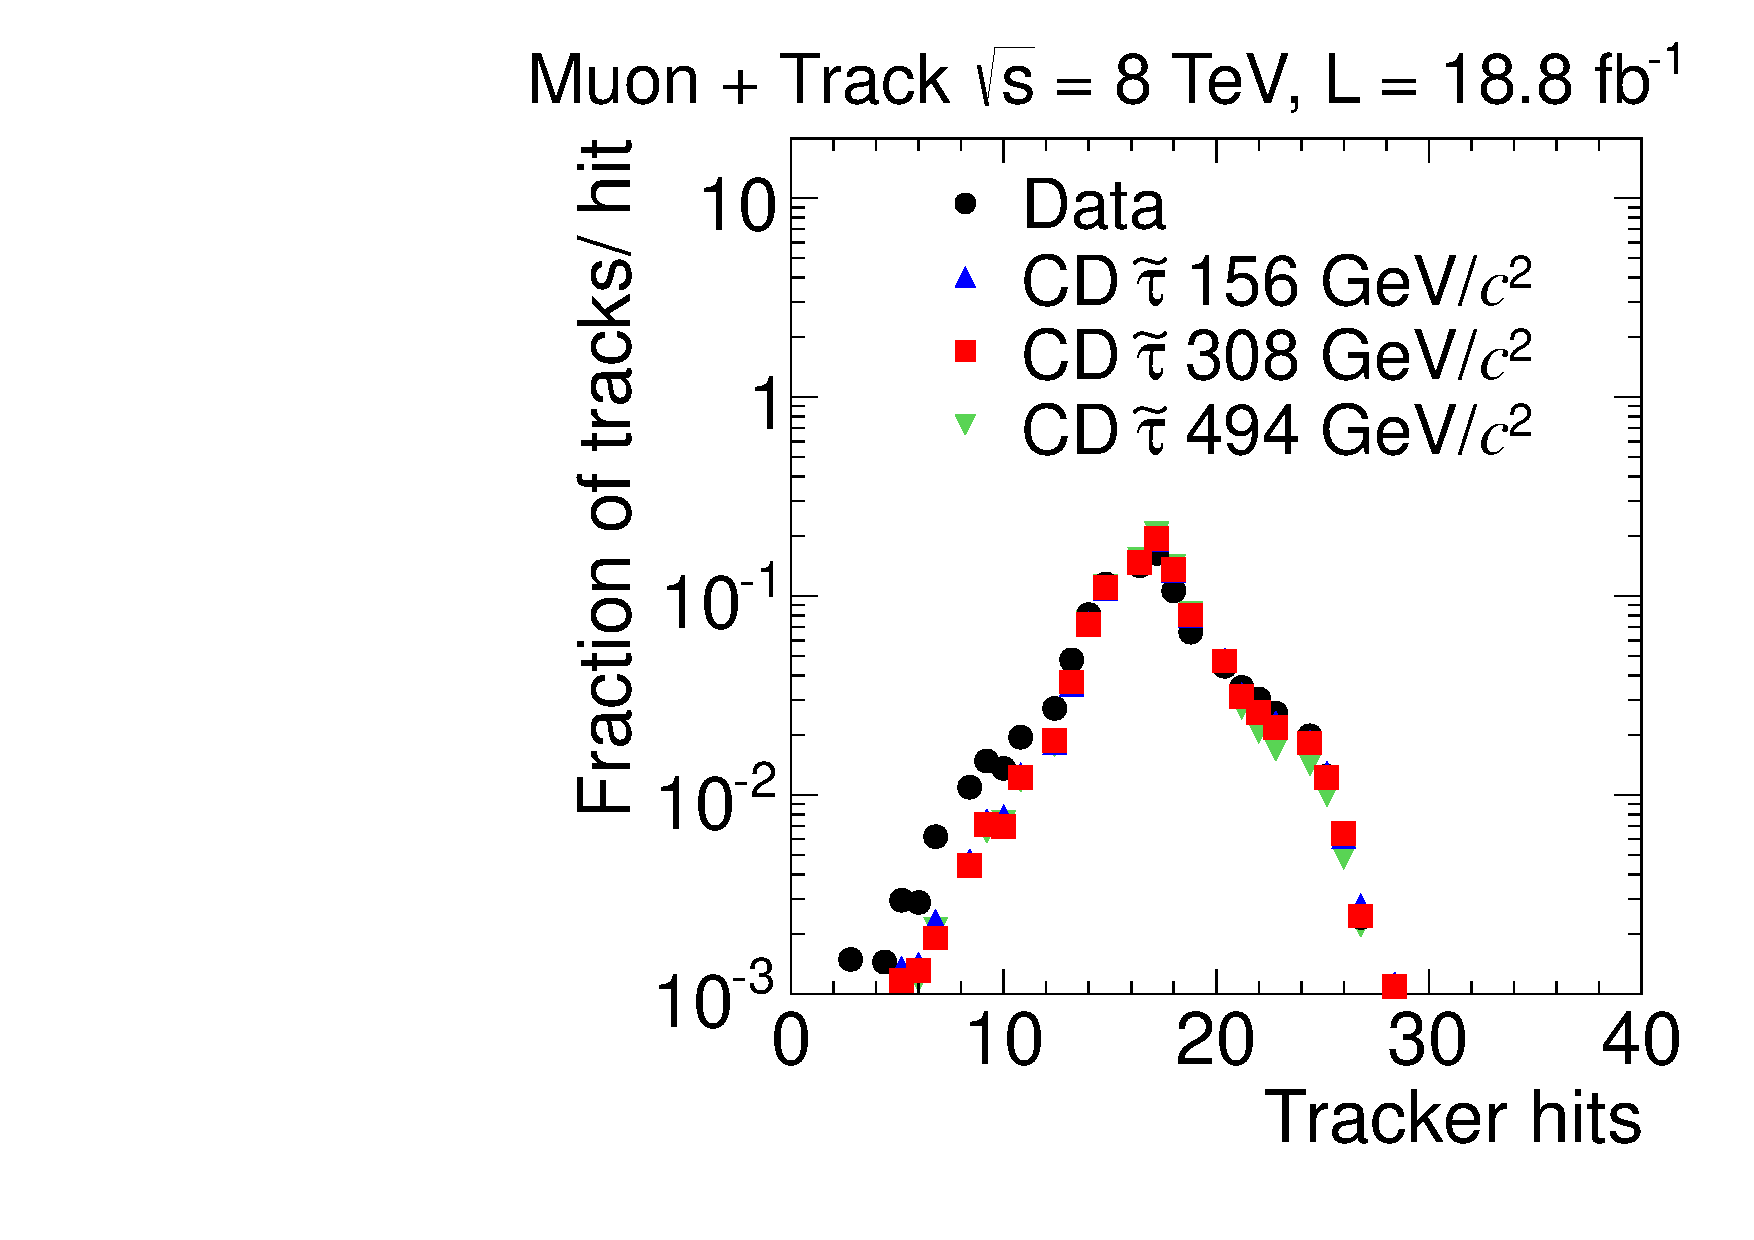
\includegraphics[clip=true, trim=0.0cm 0cm 2.8cm 0cm, width=0.44\textwidth]{figures/tkmu/Selection_Comp_8TeV_GMStau_NOH_BS}
  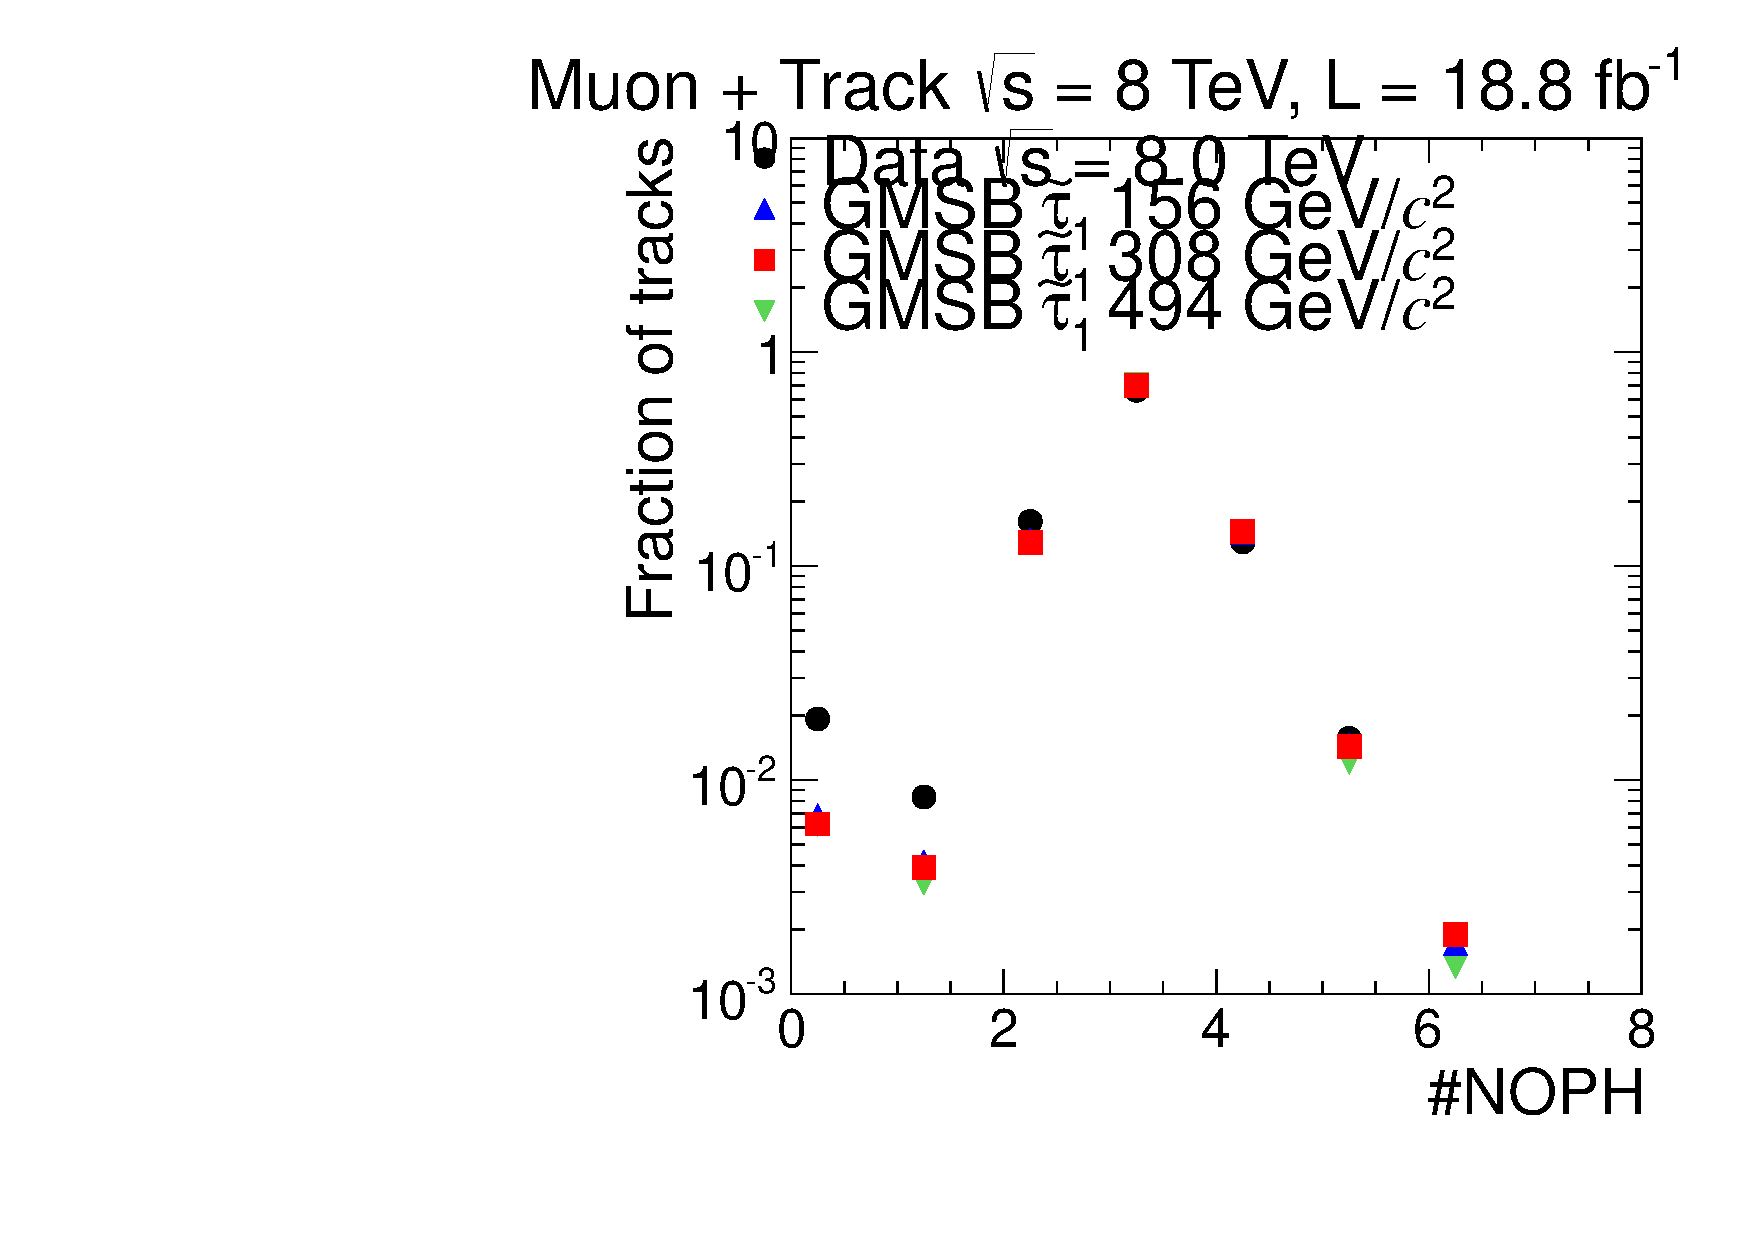
\includegraphics[clip=true, trim=0.0cm 0cm 2.8cm 0cm, width=0.44\textwidth]{figures/tkmu/Selection_Comp_8TeV_GMStau_NOPH_BS} \\
  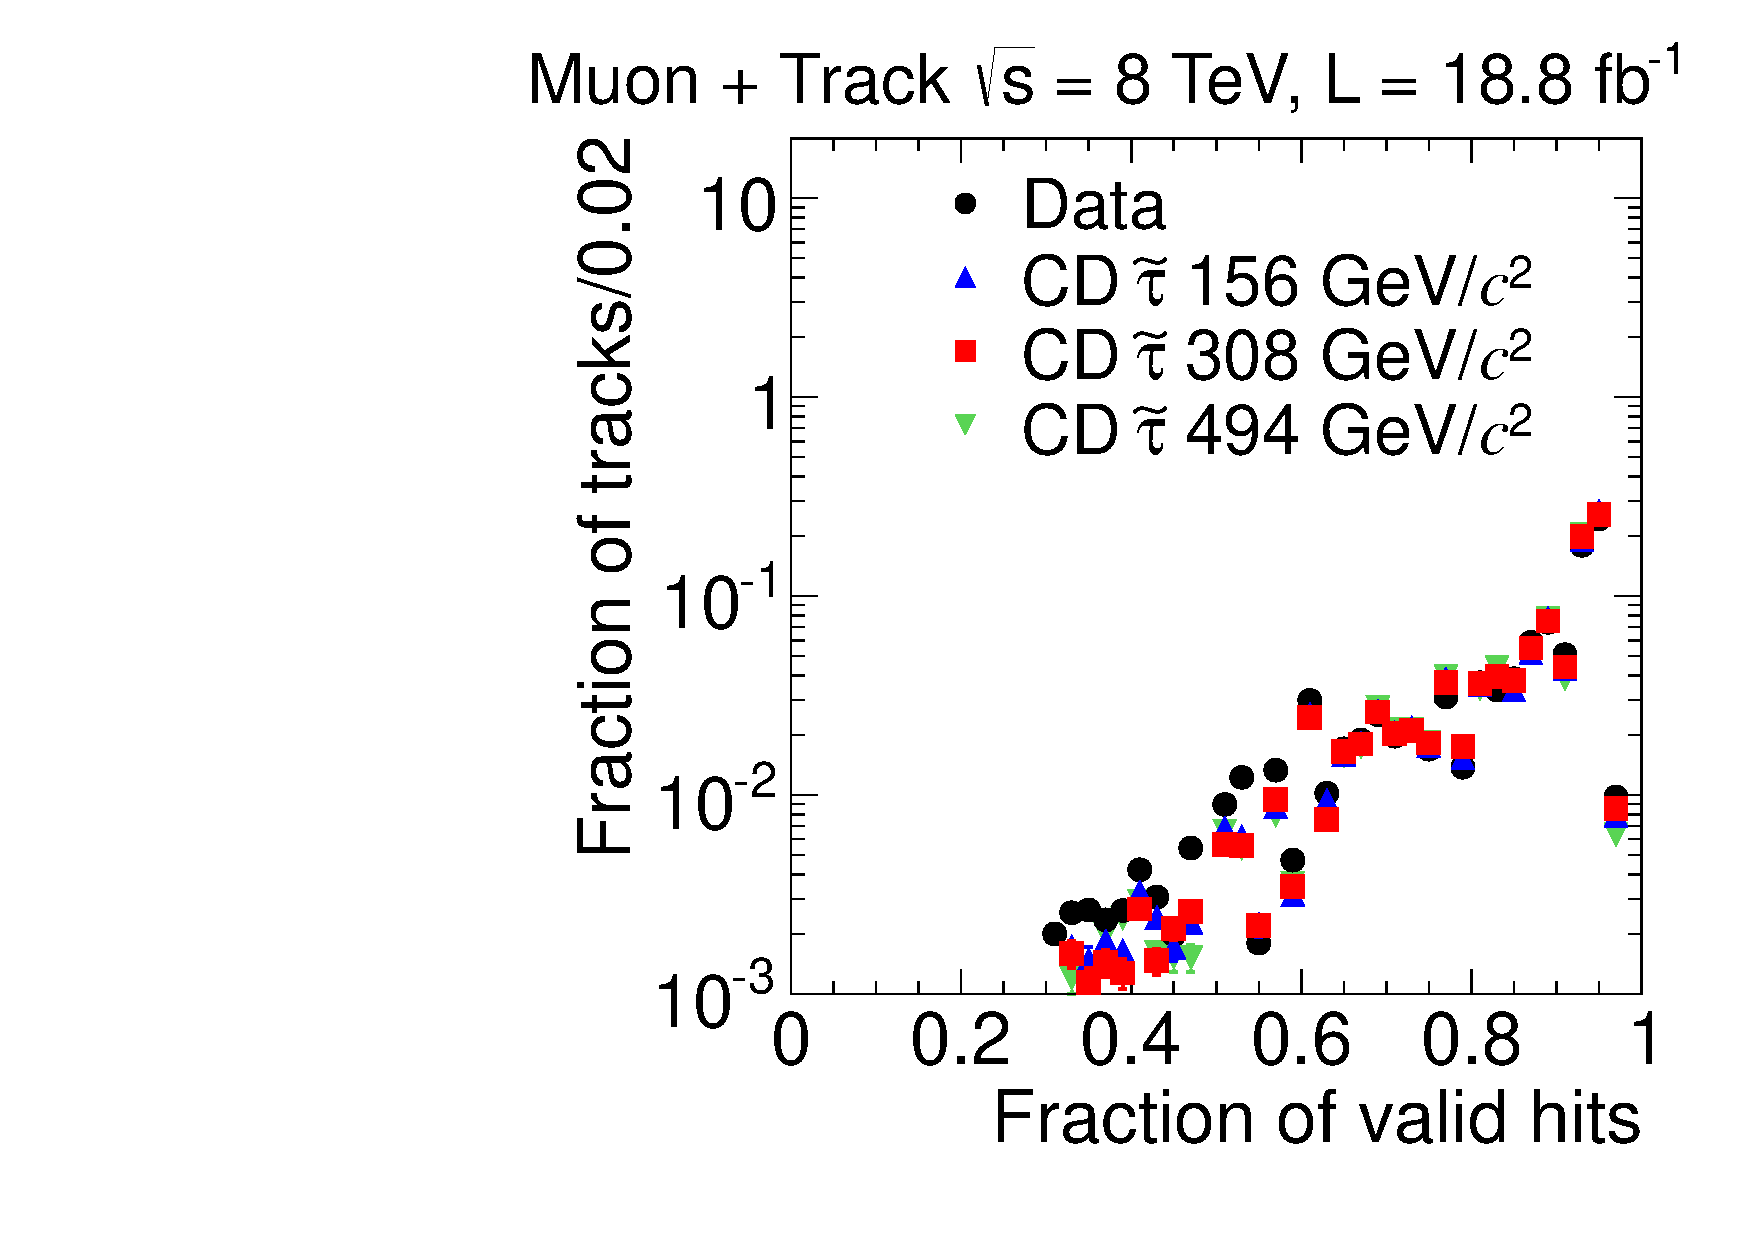
\includegraphics[clip=true, trim=0.0cm 0cm 2.8cm 0cm, width=0.44\textwidth]{figures/tkmu/Selection_Comp_8TeV_GMStau_NOHFraction_BS}
  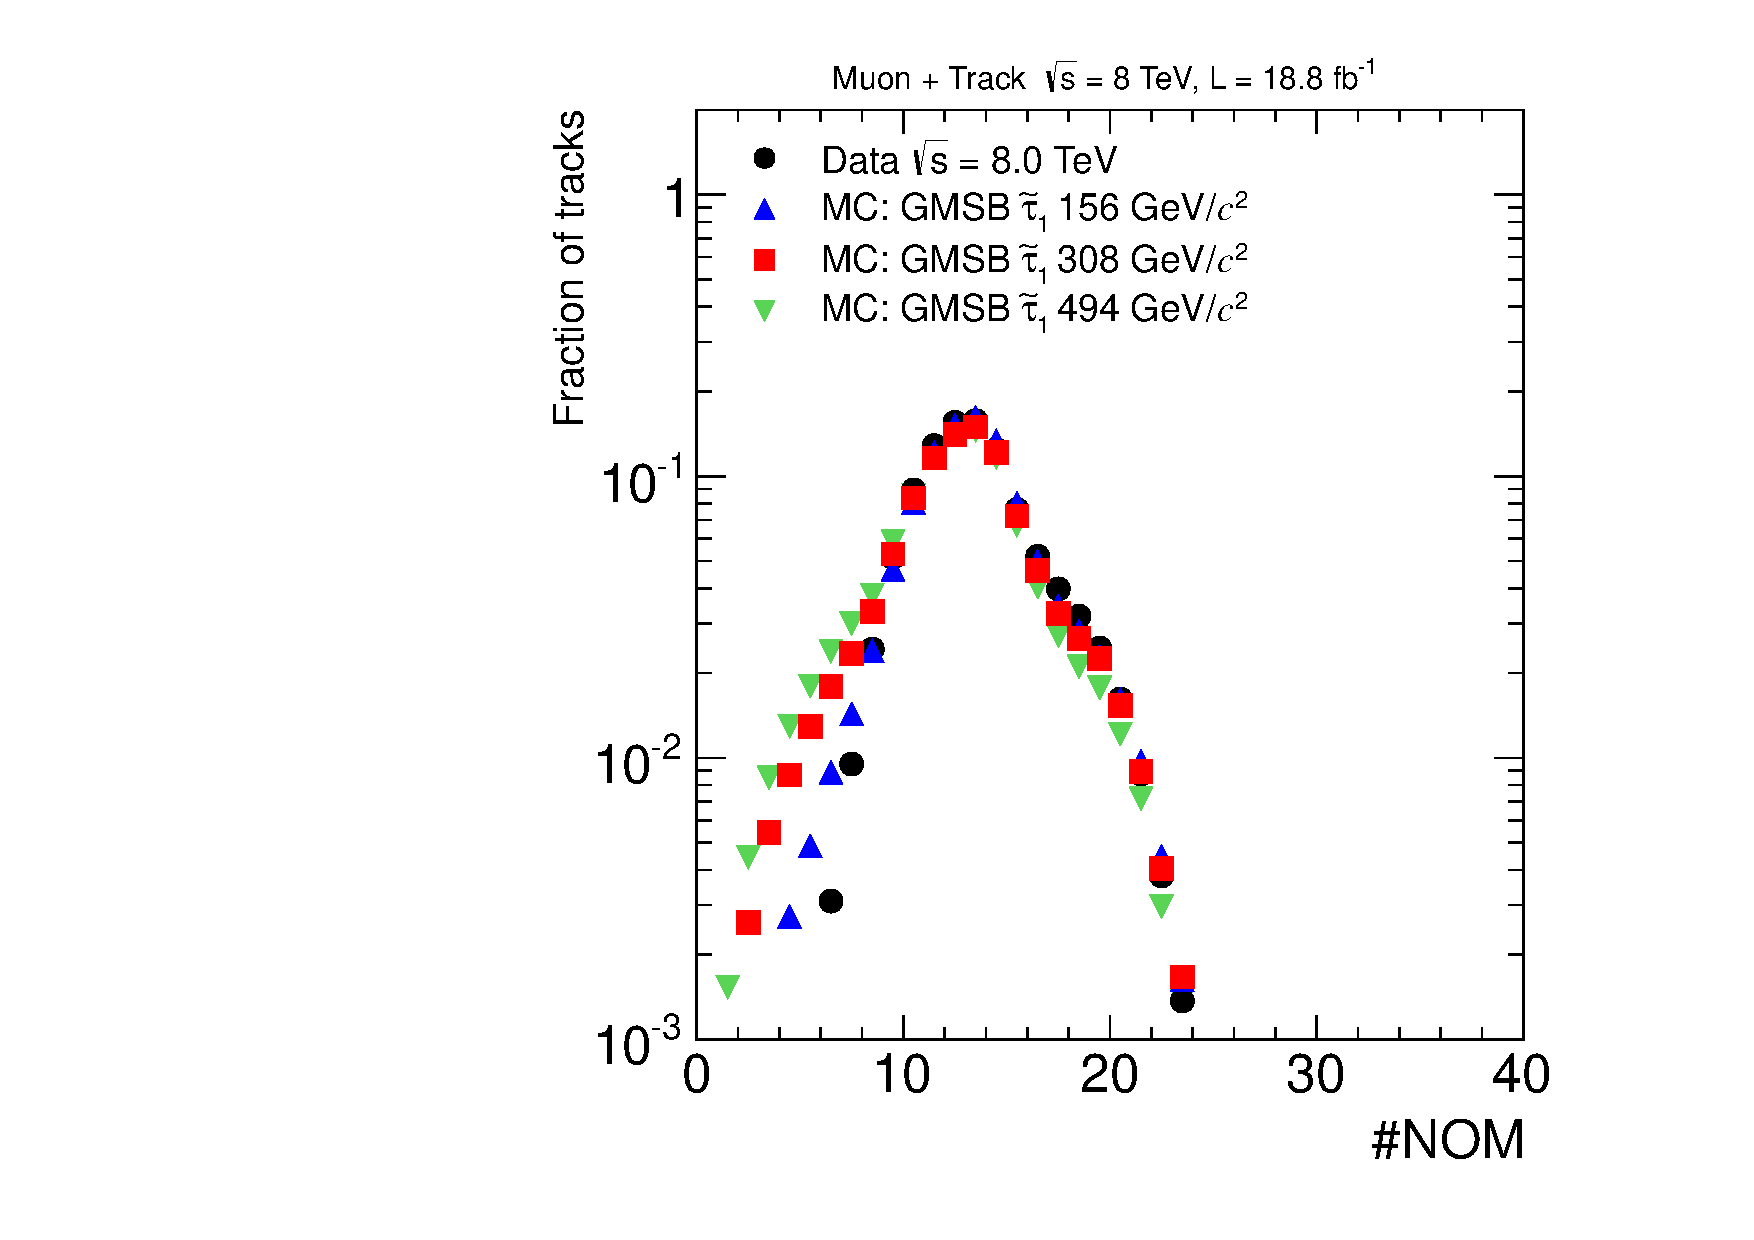
\includegraphics[clip=true, trim=0.0cm 0cm 2.8cm 0cm, width=0.44\textwidth]{figures/tkmu/Selection_Comp_8TeV_GMStau_NOM_BS}
  \caption{Distribution of various prelection variables for data and signal MC.
Top row: Number of tracker (left) and pixel (right) hits.
Bottom row: Fraction of valid tracker hits (left) and number of measurements used for \dedx\ calculation (right).
    \label{fig:TkMuPreselA}}
\end{figure}

The relative error on the candidate $p_T$ ($\sigma_{p_T}/p_T$) must be less than 0.25 and the $\chi^2$ per degree of freedom must be less than five.
While cosmics are expected to be a negligible background in the \tktof\ analysis loose cuts are placed on the impact parameter of the track, 
these cuts are nearly 100\% efficient for signal particles.
The displacement of the track with respect to the primary vertex
with the smallest longitudinal displament must be less than 0.5 in both the transverse and longitudinal directions.
Figure~\ref{fig:TkMuPreselB} shows $p_T$ error, $\chi^2$ per degree of freedom, and the $d_z$ and $d_{xy}$ displacement for data and signal MC.

\begin{figure}
\centering
  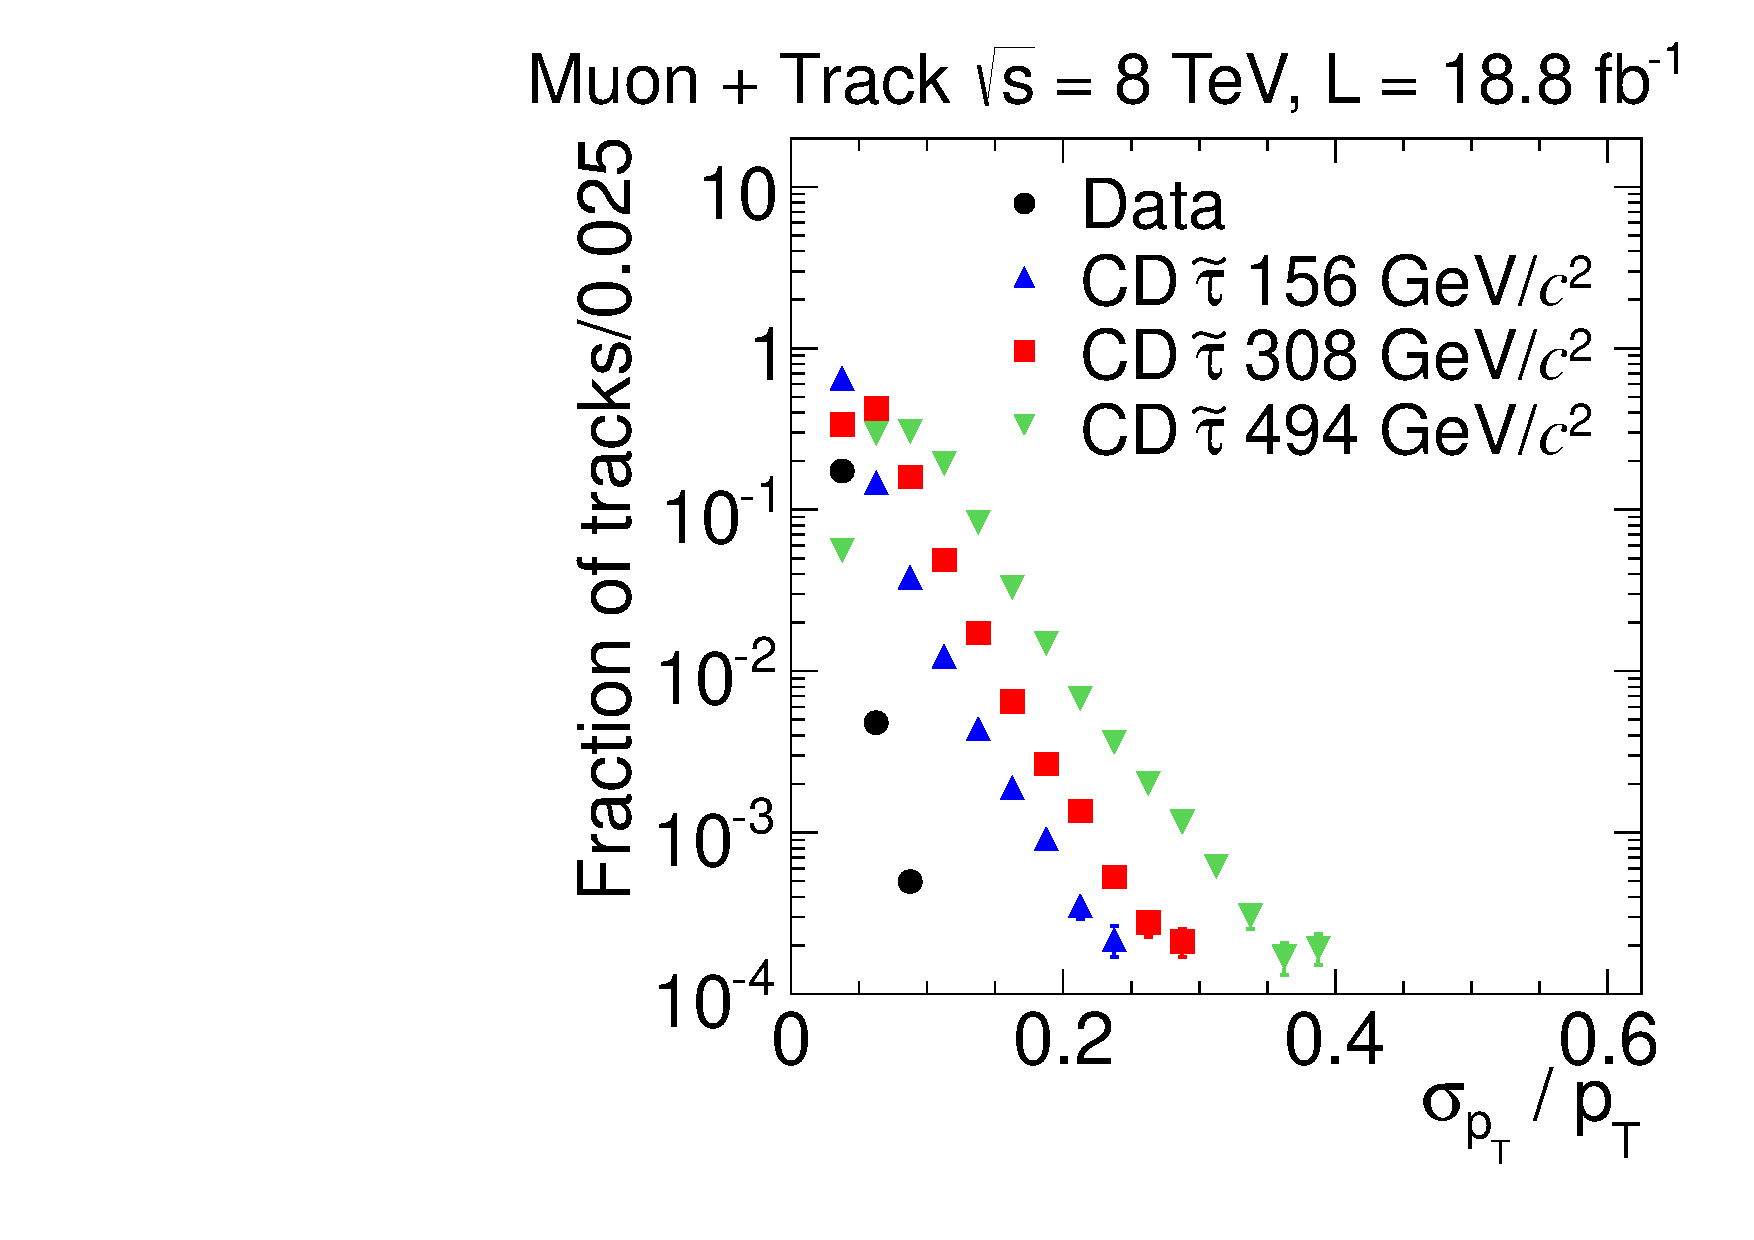
\includegraphics[clip=true, trim=0.0cm 0cm 2.8cm 0cm, width=0.44\textwidth]{figures/tkmu/Selection_Comp_8TeV_GMStau_Pterr_BS}
  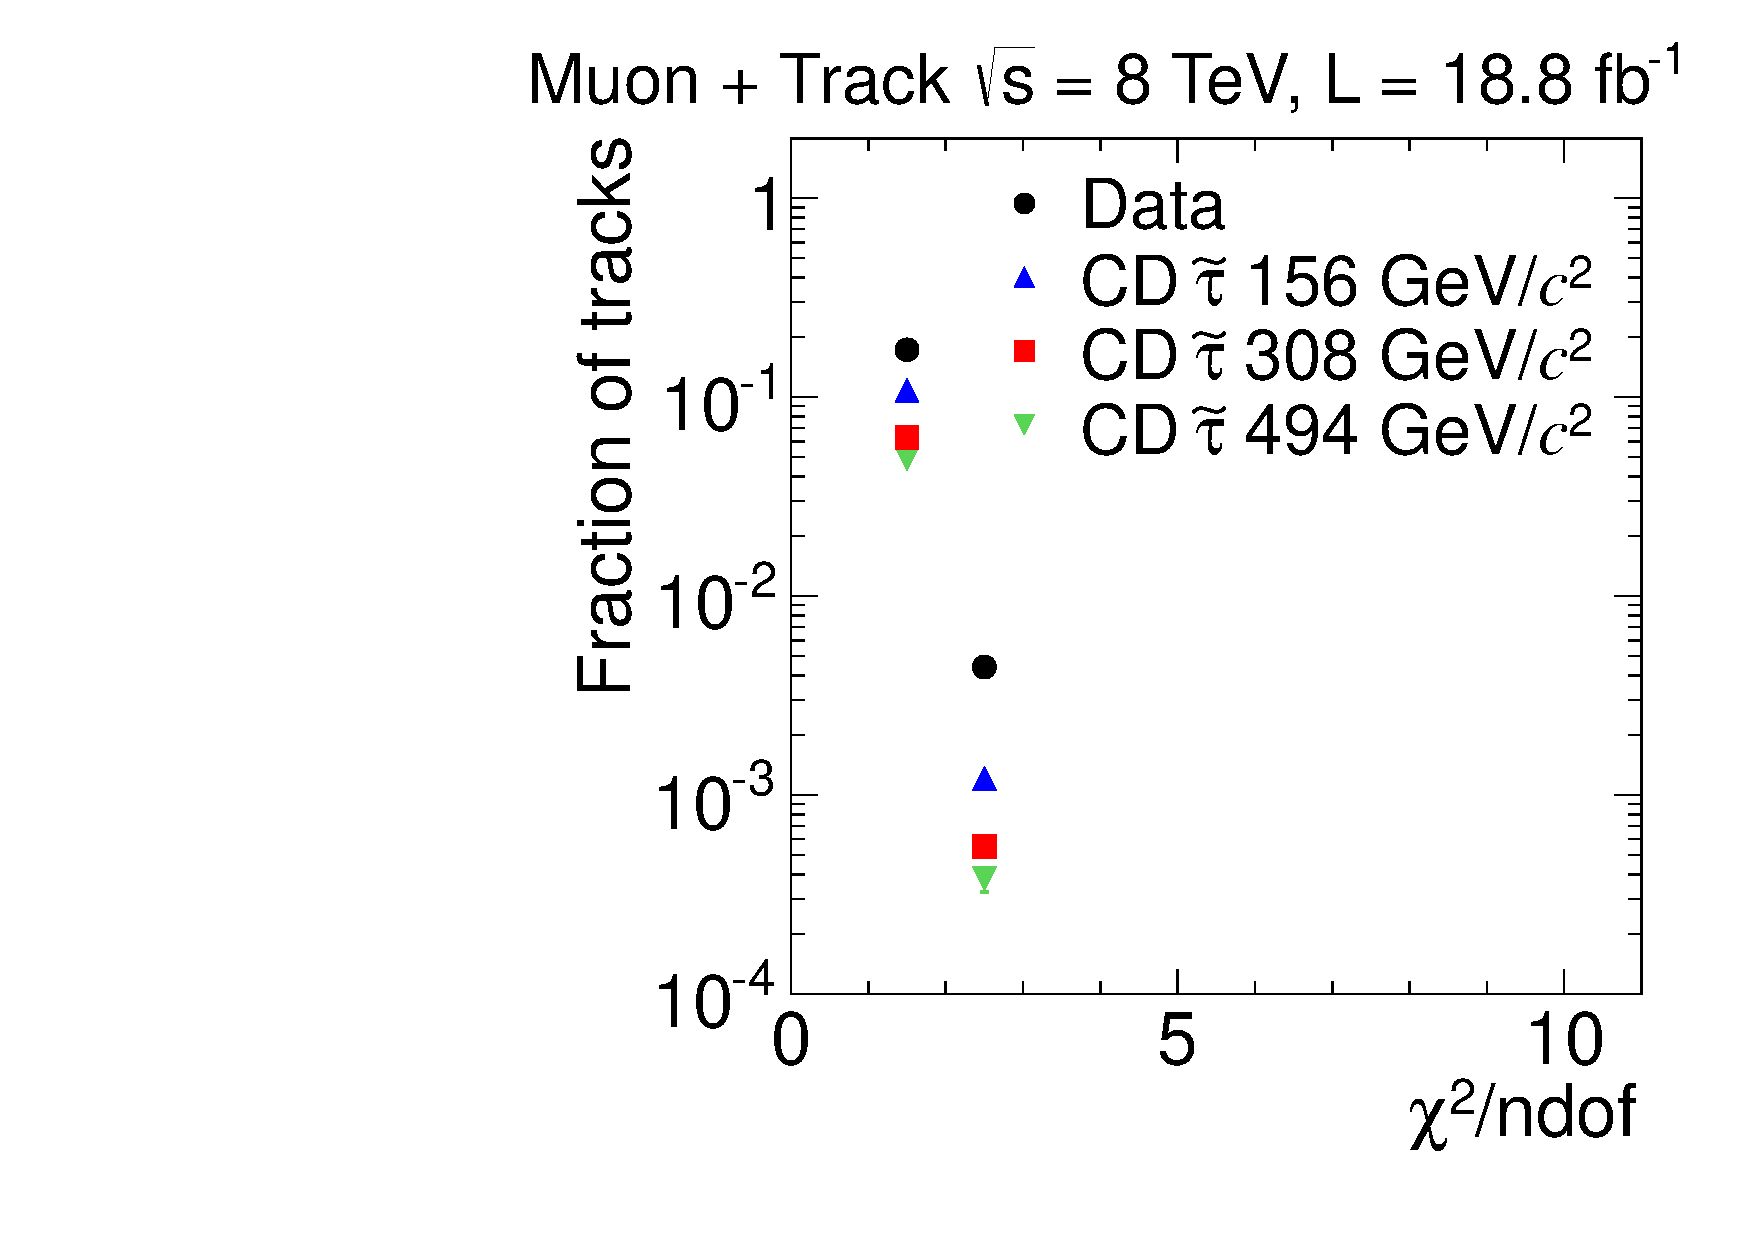
\includegraphics[clip=true, trim=0.0cm 0cm 2.8cm 0cm, width=0.44\textwidth]{figures/tkmu/Selection_Comp_8TeV_GMStau_Chi2_BS} \\
  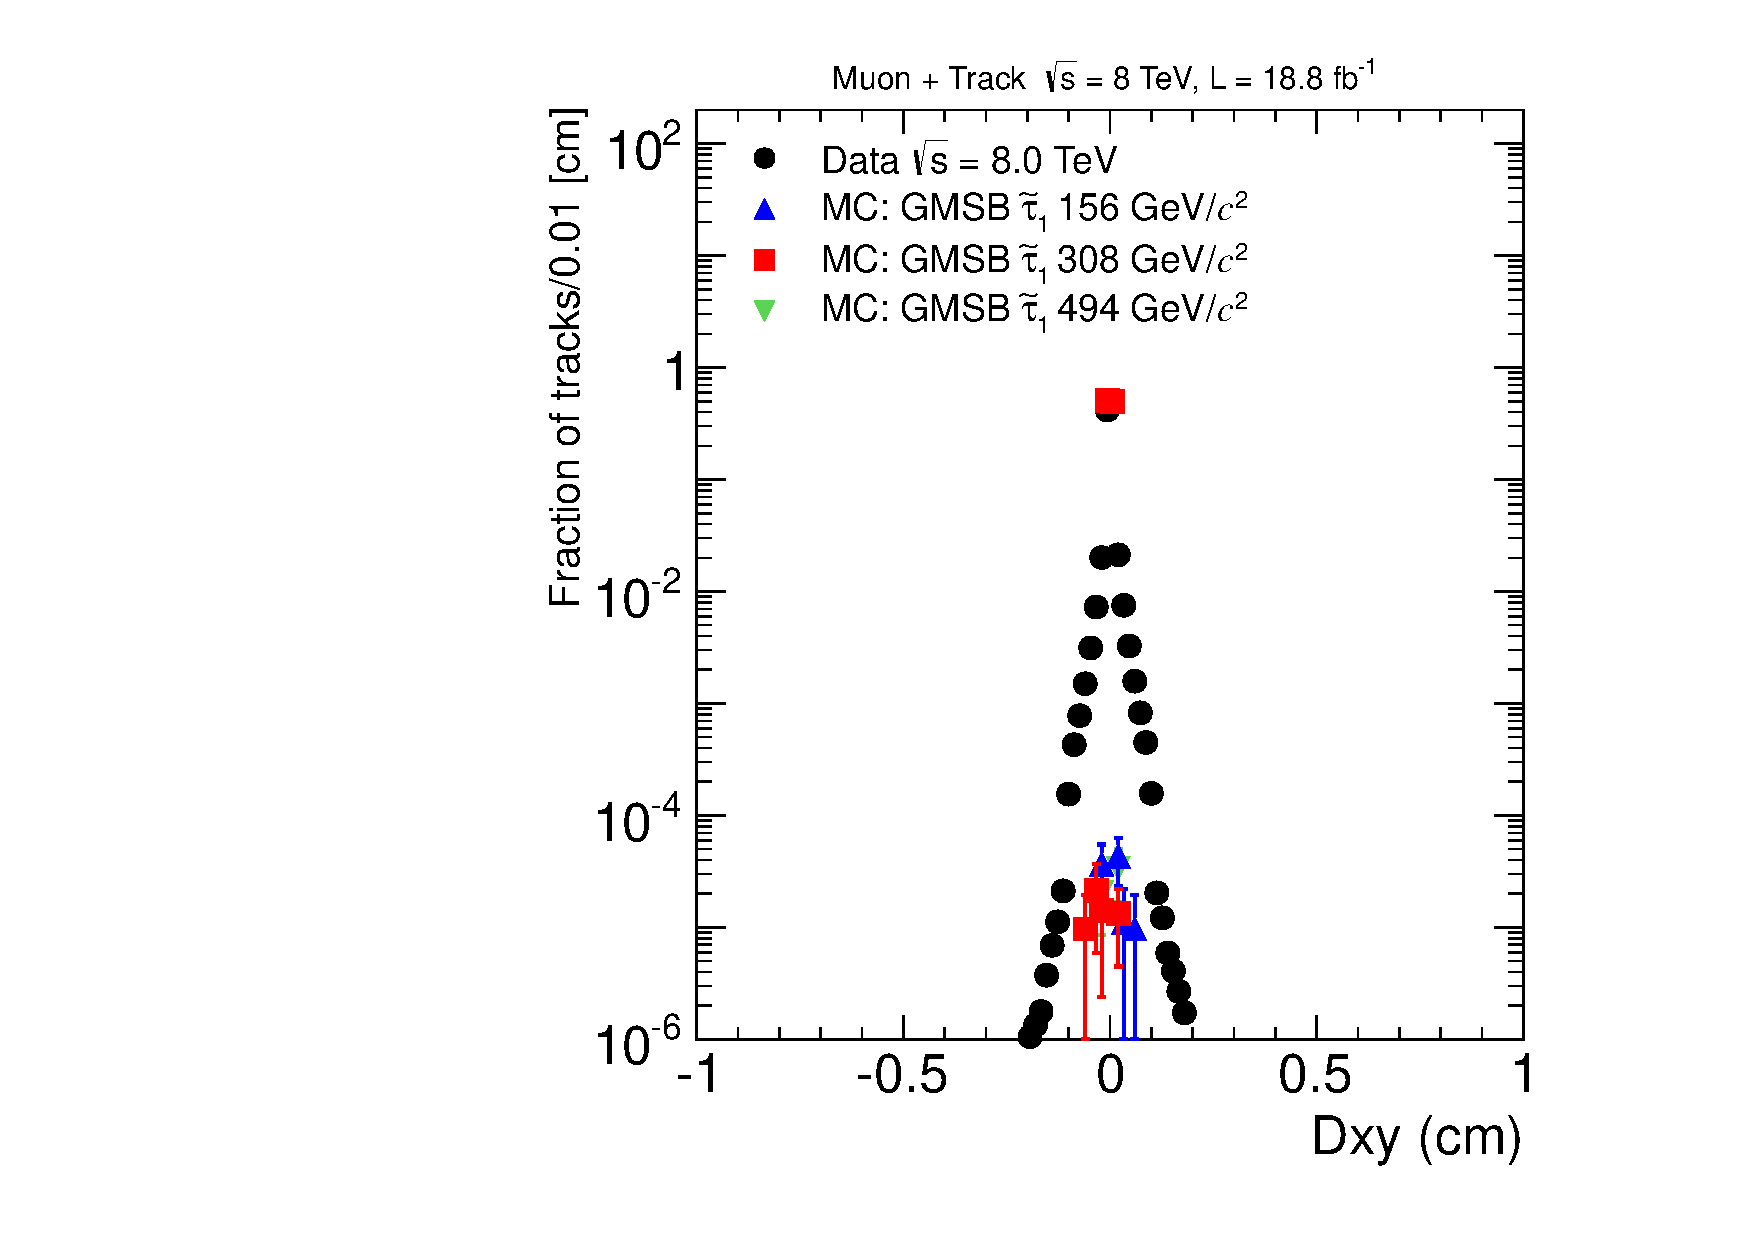
\includegraphics[clip=true, trim=0.0cm 0cm 2.8cm 0cm, width=0.44\textwidth]{figures/tkmu/Selection_Comp_8TeV_GMStau_Dxy_BS}
  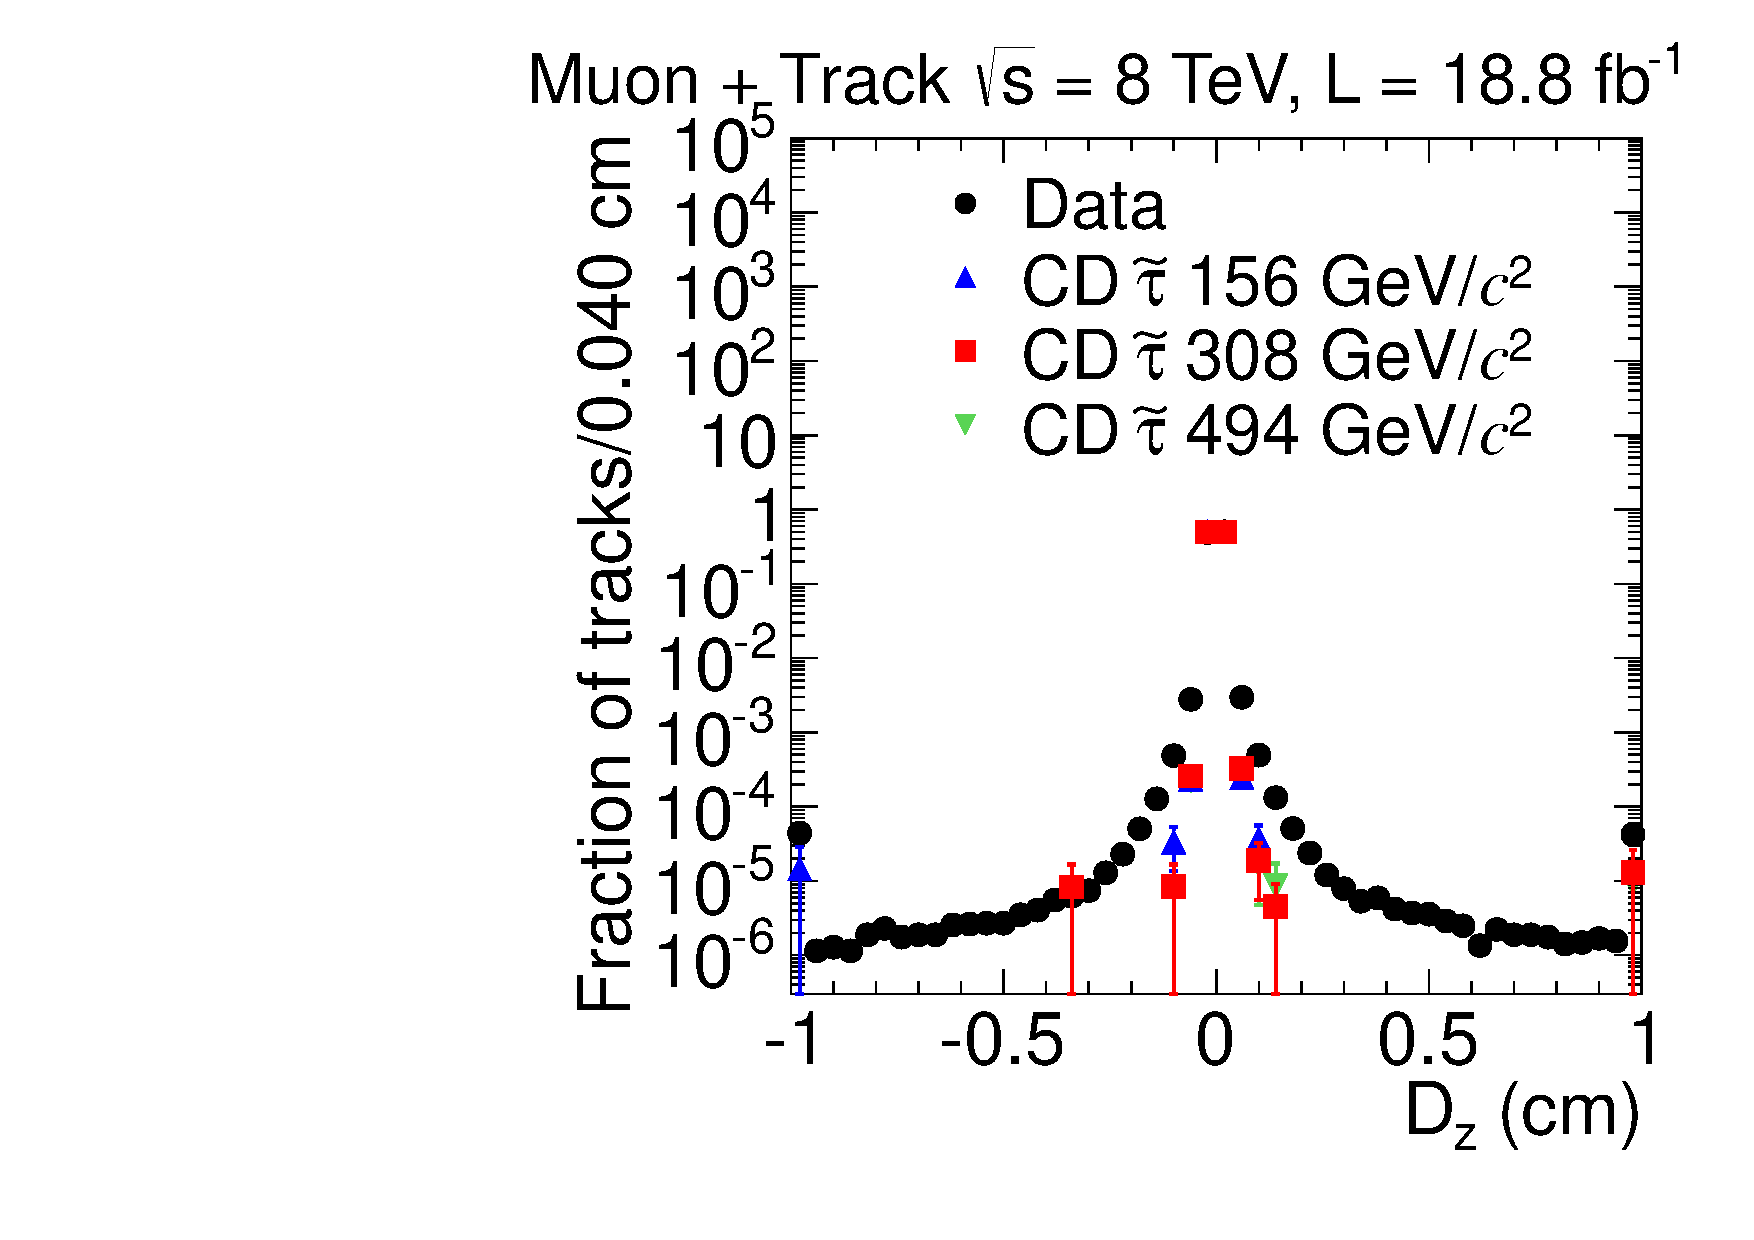
\includegraphics[clip=true, trim=0.0cm 0cm 2.8cm 0cm, width=0.44\textwidth]{figures/tkmu/Selection_Comp_8TeV_GMStau_Dz_BS}
  \caption{Distribution of various prelection variables for data and signal MC.
Top row: Relative $p_T$ error (left) and $\chi^2$ per degree of freedom (right).
Bottom row: Displacement in the transverse (left) and longitudinal (right) directions.
    \label{fig:TkMuPreselB}}
\end{figure}

The candidates for the \tktof\ analysis are also required to be isolated to reduce QCD production of jets where overlapping tracks could give
anomolously high \dedx\ values. The isolation cuts are kept very loose as slow moving HSCP will deposit more energy in the calorimeter than a SM particle.
The sum of the momentum of the tracks within 0.3 of the candidate (excluding the candidate itself) is required to be less than 50 GeV. Additionally the total
amount of energy measured in the calorimeter within a radius of 0.3 to the candidate divided by the candidate momentum must be less than 0.3.

Additionally, the \tktof\ analysis uses the same cuts on the \invbeta\ error and number of measurements as the \muononly\ analysis.
Figure~\ref{fig:TkMuPreselC} shows the isolation and \invbeta\ variables for data and signal MC.

\begin{figure}
\centering
  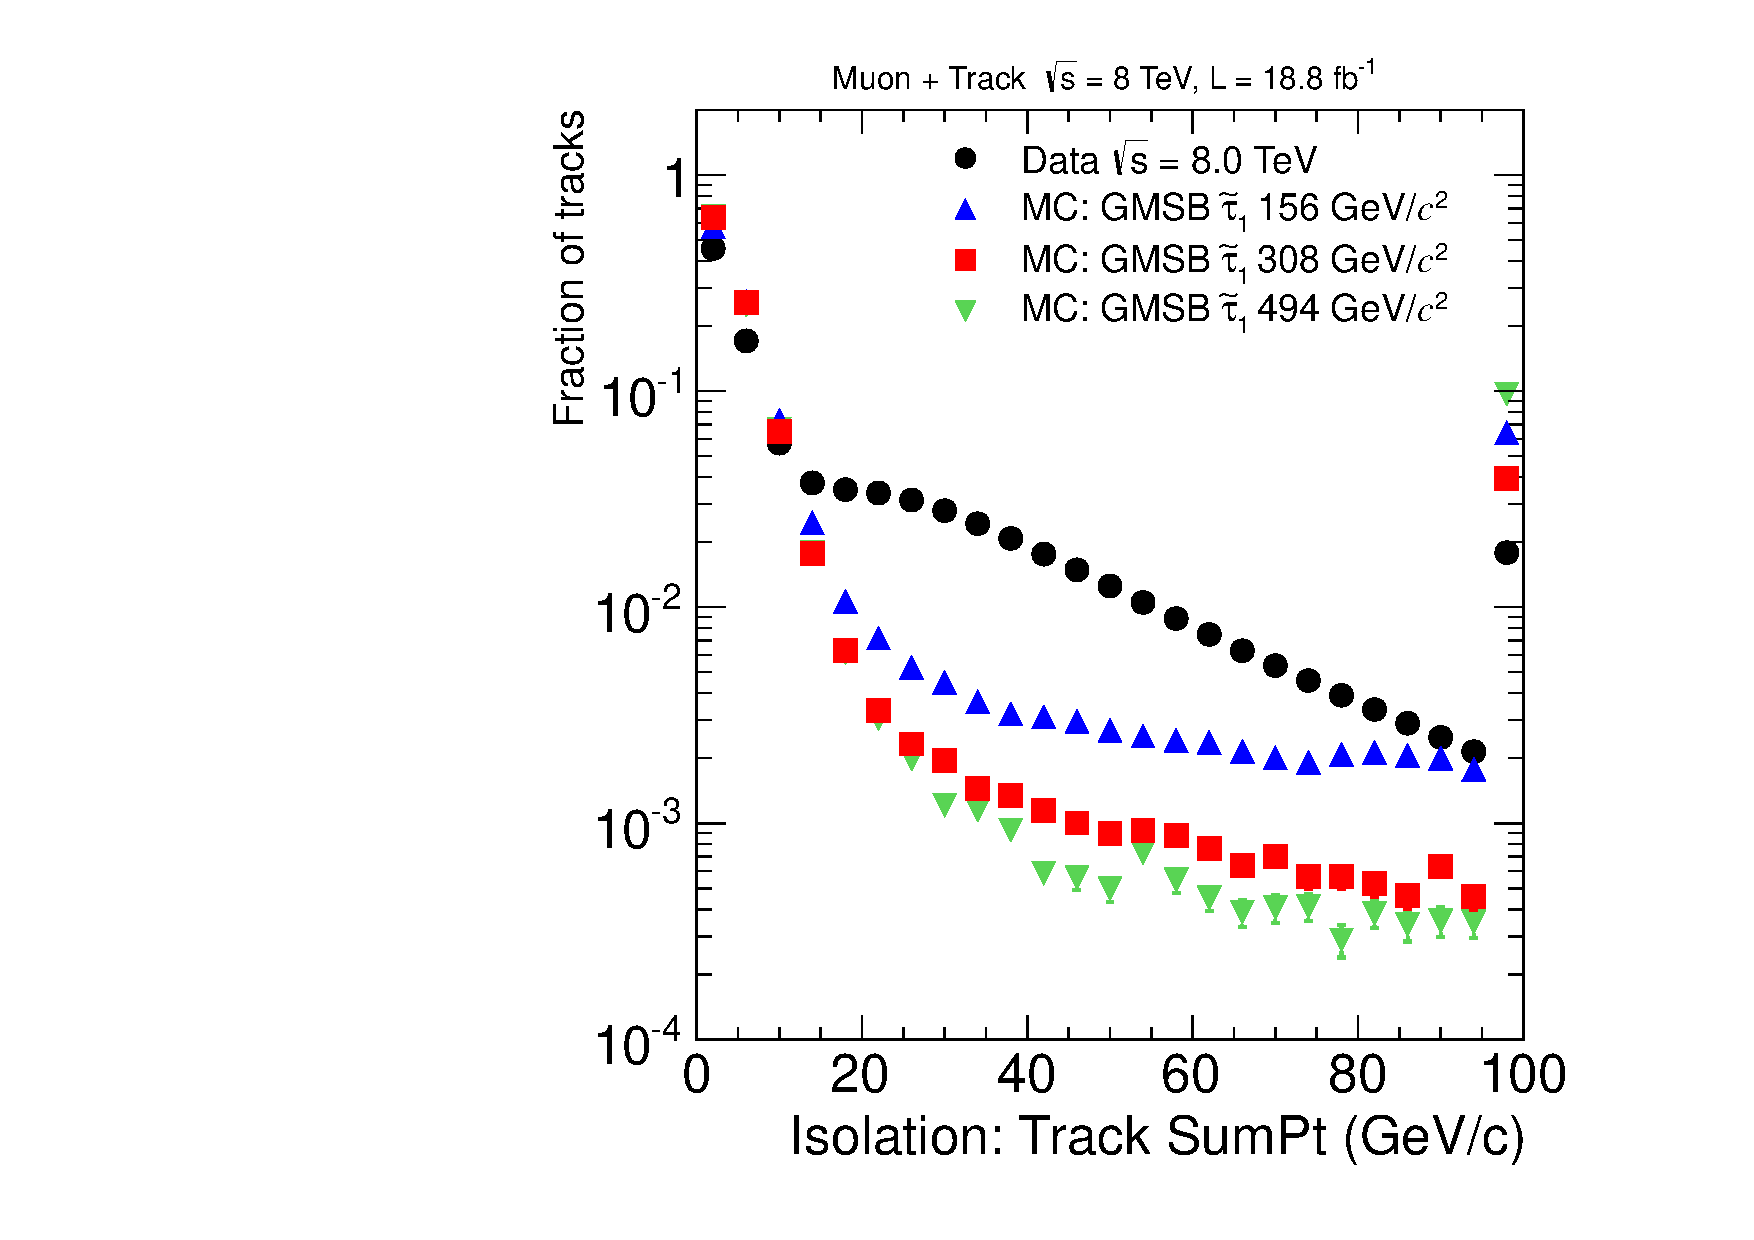
\includegraphics[clip=true, trim=0.0cm 0cm 2.8cm 0cm, width=0.44\textwidth]{figures/tkmu/Selection_Comp_8TeV_GMStau_IsolT_BS}
  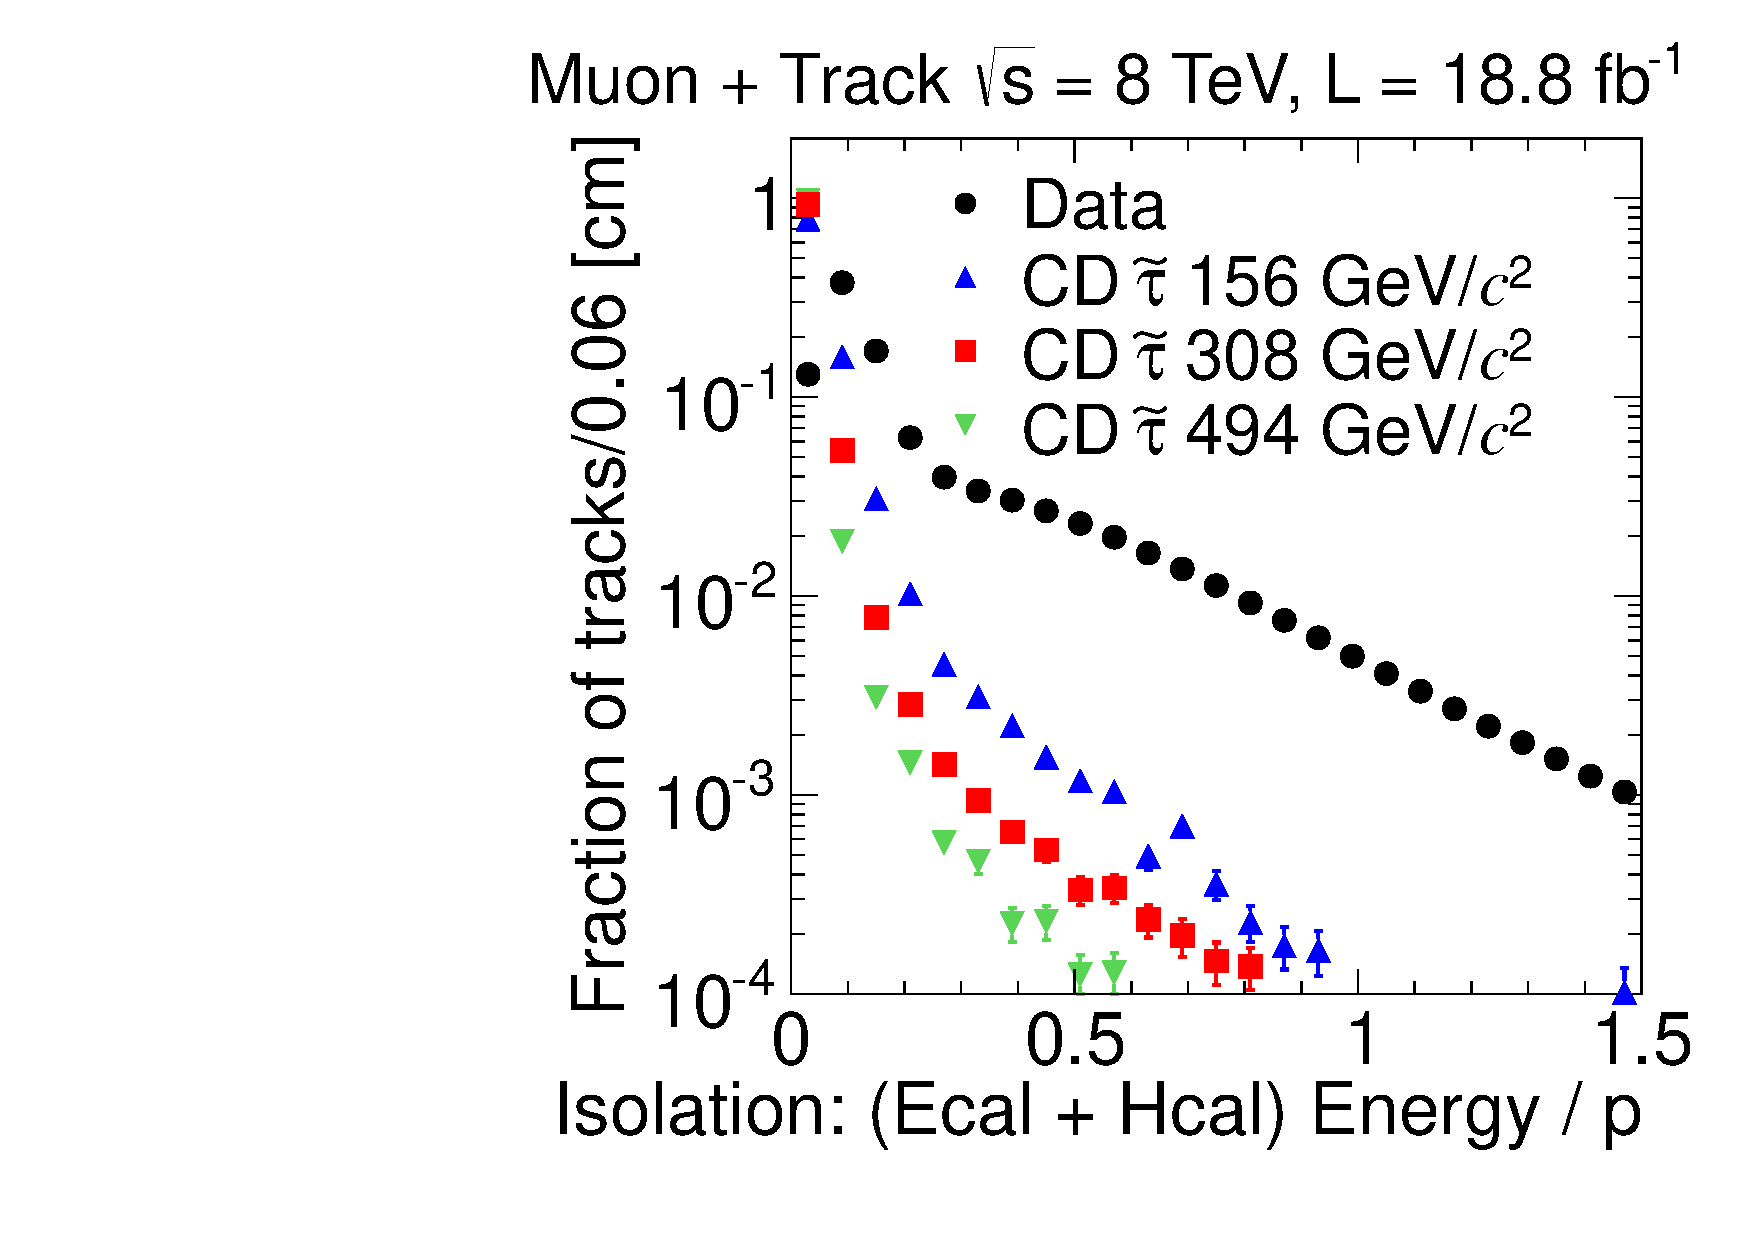
\includegraphics[clip=true, trim=0.0cm 0cm 2.8cm 0cm, width=0.44\textwidth]{figures/tkmu/Selection_Comp_8TeV_GMStau_IsolE_BS} \\
  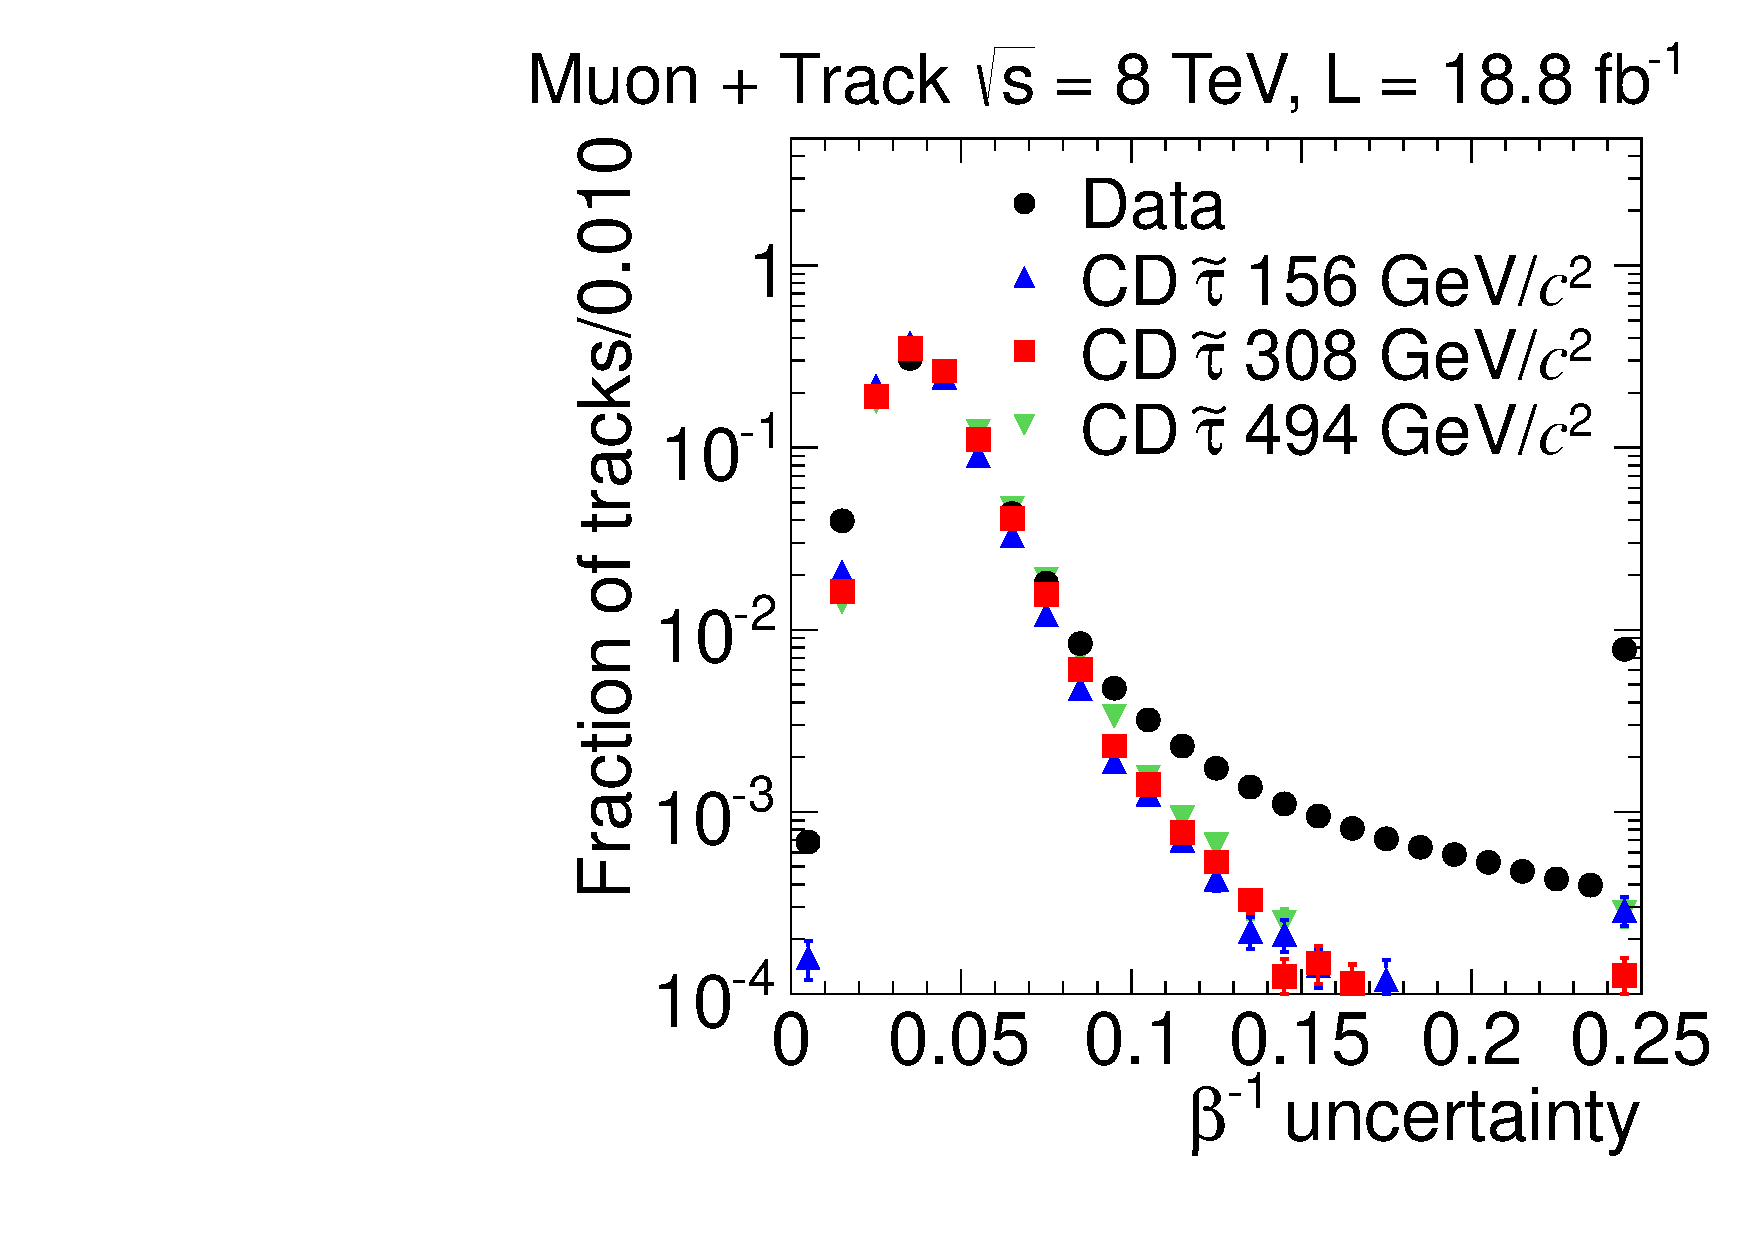
\includegraphics[clip=true, trim=0.0cm 0cm 2.8cm 0cm, width=0.44\textwidth]{figures/tkmu/Selection_Comp_8TeV_GMStau_TOFError_BS}
  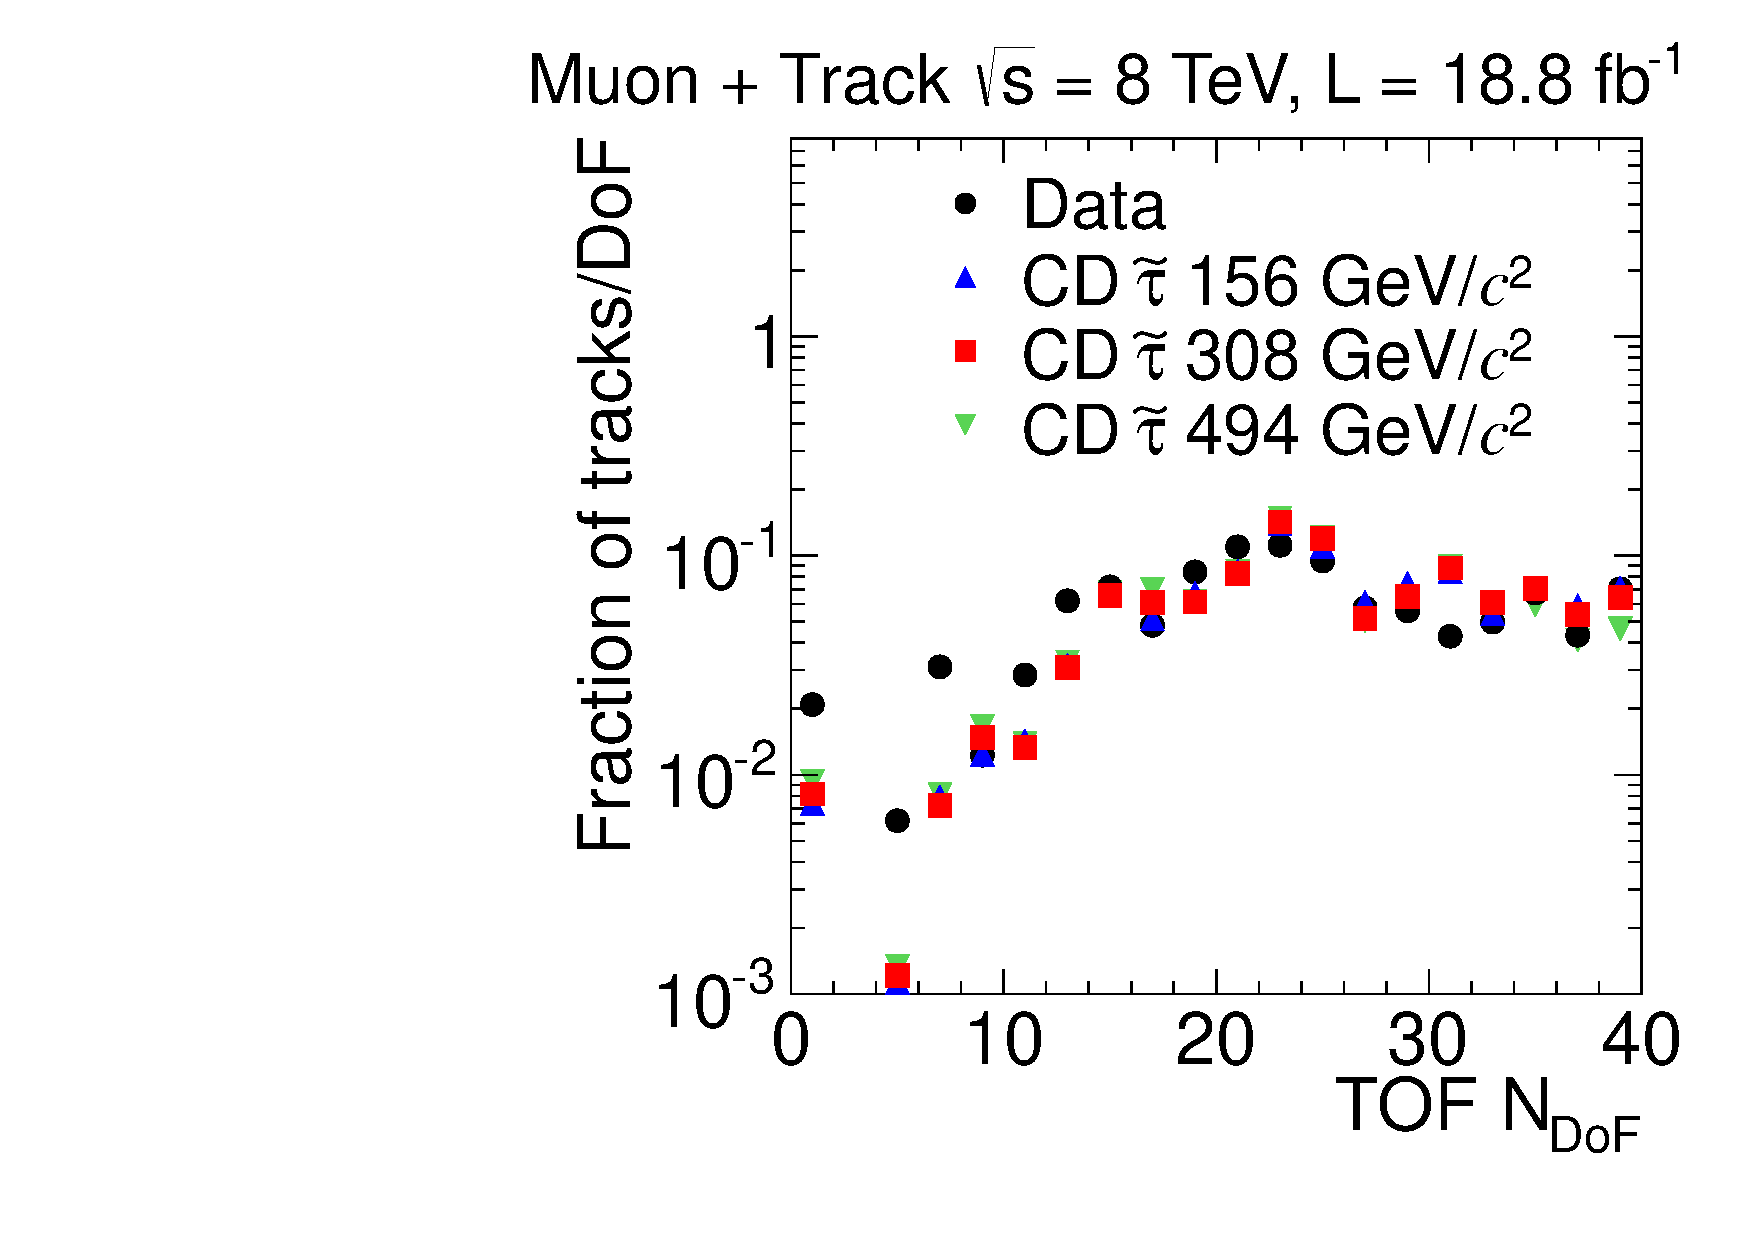
\includegraphics[clip=true, trim=0.0cm 0cm 2.8cm 0cm, width=0.44\textwidth]{figures/tkmu/Selection_Comp_8TeV_GMStau_nDof_BS}
  \caption{Distribution of various prelection variables for data and signal MC.
Top row: Sum momentum of tracks within 0.3 (left) and calorimeter energy within 0.3 divided by track momentum.
Bottom row: Distribution of the \invbeta\ measurement error (left) and the number of degrees of freedom (right).
    \label{fig:TkMuPreselC}}
\end{figure}

The \tkonly\ analysis applies the same preselection as the \tktof\ analysis except the cuts on the timing measurement are not applied as the candidates
are not required to be reconstructed in the muon system. The \fract\ analysis uses preselection like \tkonly\ but inverting the \ih\ requirement
to be less than 2.8 and requiring no tracks with \pt\ greater than 45 GeV to have an opening angle with the candidate greater than 2.8 radians.

The \multi\ analysis applies
the same selection criteria as the \tktof\ analysis except the cut on relative isolation less than 0.3 and the cleaning of the hits used for the \dedx\ calculation
is not done. The cleaning procedure is not applied because the amount of charge deposited is proportionalt $Q^2$ meaning that even a $Q=2e$ HSCP will
deposit four times as much charge as a $Q=1e$ HSCP. As the tracker saturates for a charge ~3 times that expected for a MIP many of the hits from $Q>1e$ HSCP
will be saturated and this can confuse the cleaning procedure. Additionally, as the high charge samples deposit so much charge, 
there will still be good signal/background separation even with longer tails in the \dedx\ distribution.
Figure~\ref{fig:TkMuPreselC} shows the number of measurements passing the cleaning for multiply charged samples and the opening
angle described above for fractionally charged samples.

\begin{figure}
\centering
  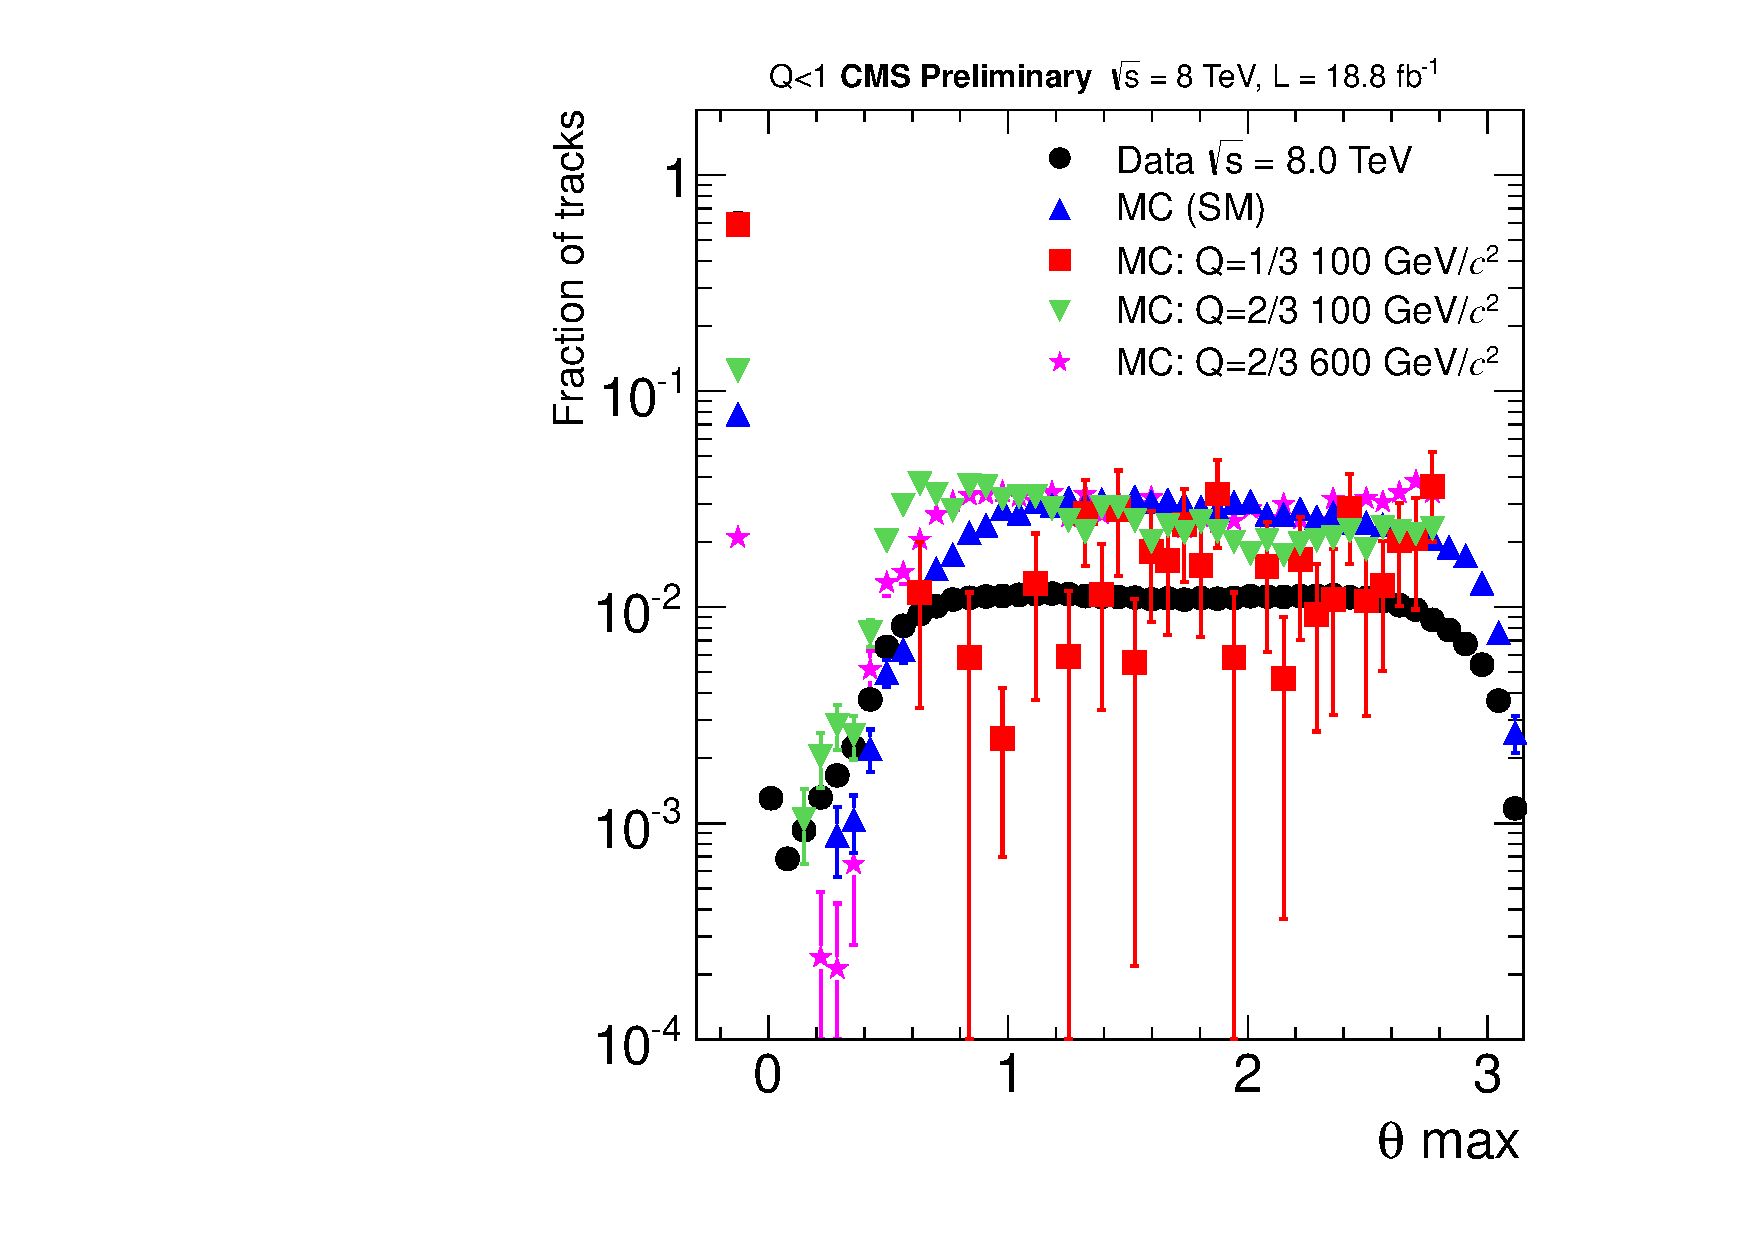
\includegraphics[clip=true, trim=0.0cm 0cm 2.8cm 0cm, width=0.44\textwidth]{figures/fract/Selection_Comp_8TeV_DY_OpenAngle_BS}
  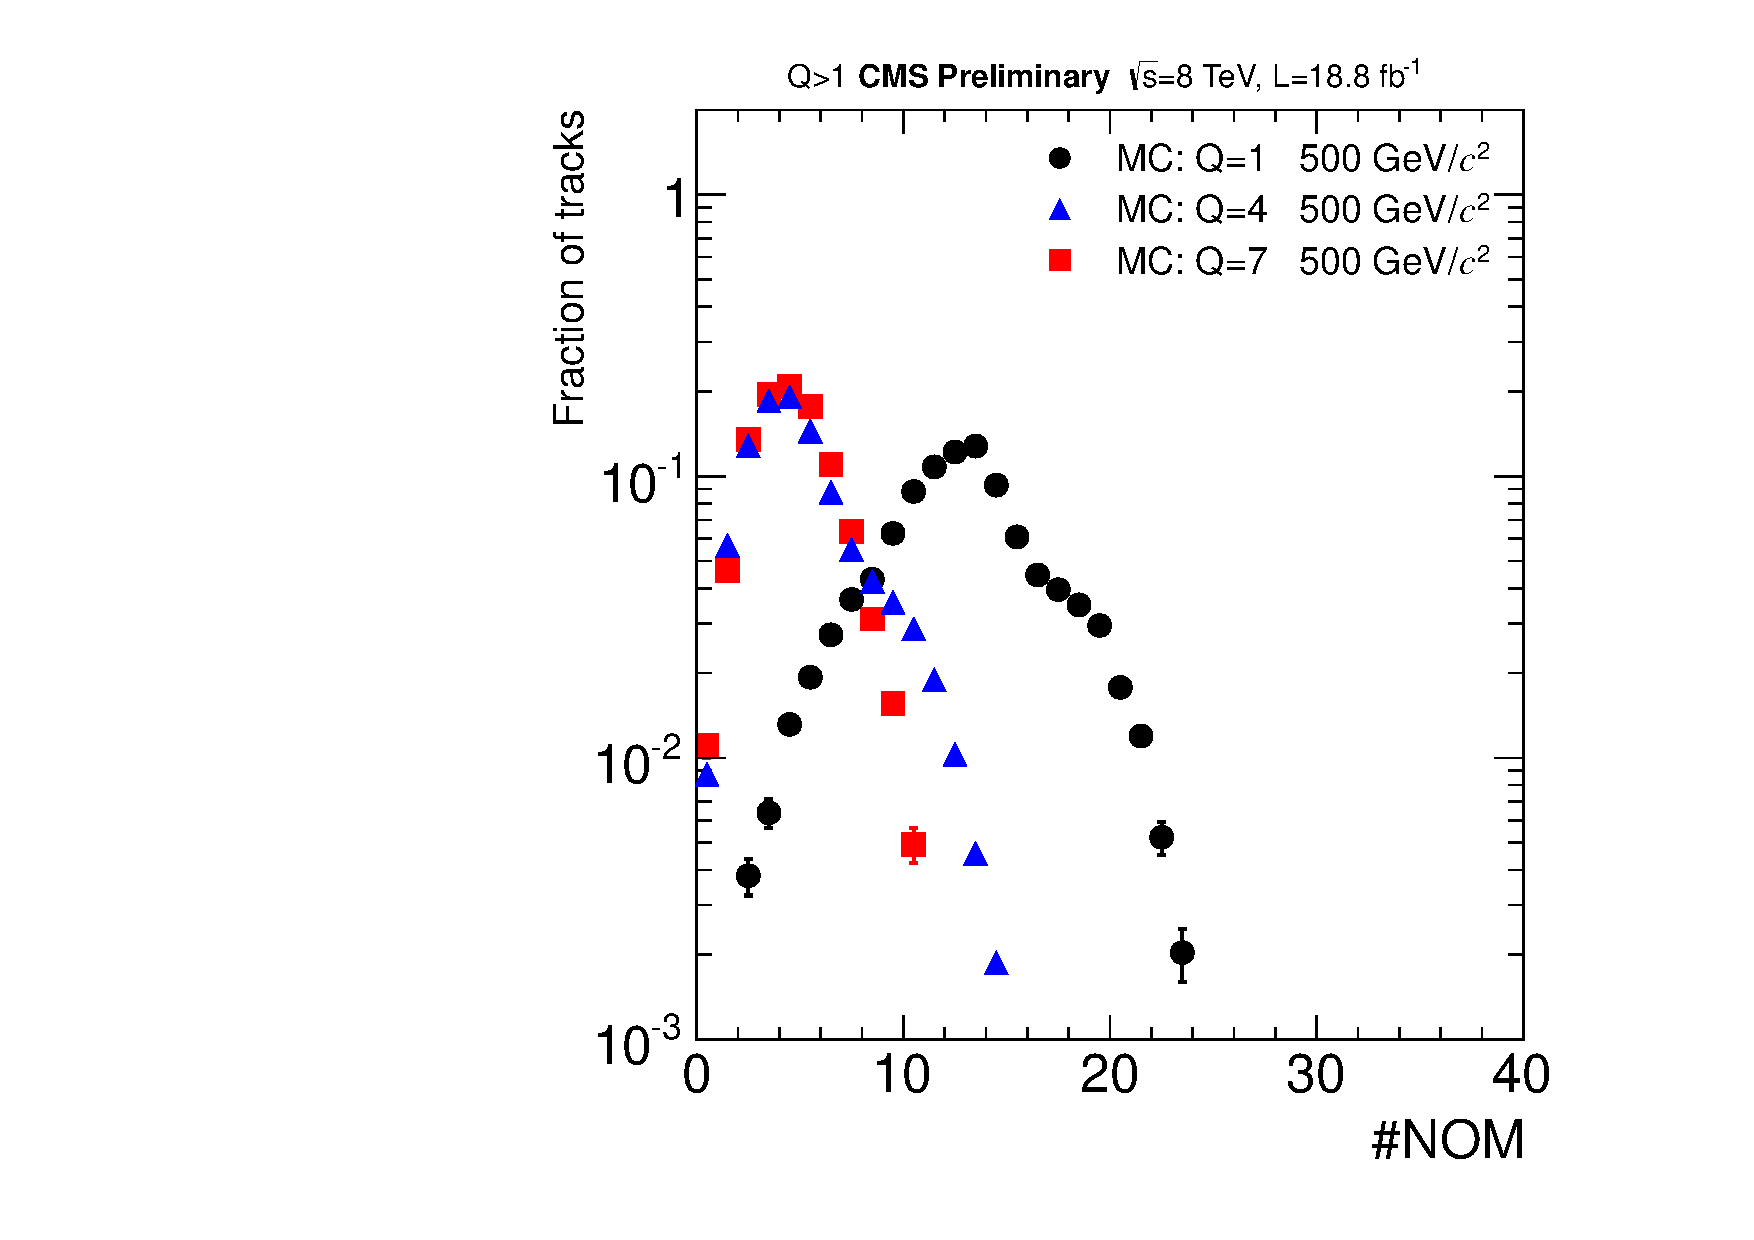
\includegraphics[clip=true, trim=0.0cm 0cm 2.8cm 0cm, width=0.44\textwidth]{figures/multi/Selection_Comp_8TeV_DY_QG_NOM_BS}
  \caption{Distribution of number of measurements passing cleaning for samples of three different charges
    \label{fig:TkMuPreselC}}
\end{figure}

The total preselection efficiency is shown in Table~\ref{tab:preselectionEff}. The efficiencies are presented with respect to HSCP reconstructed as a track in CMS.
The efficiencies decrease at high mass for color charged HSCP as the HSCP track does not behave like SM particles the reconstruction assumes it to be so many of its track
qualities become low quality. The cuts are set trying to take this into account but also not allowing poorly reconstructed background tracks to enter into the signal region.


\begin{table}
 \begin{center}
  \caption{Preselection efficiency for a few benchmark samples in each analysis.  
This efficiency is with respect to the reconstructed HSCP candidate (i.e. Stand alone muon for the \tkonly\ analysis and global muon for the \tktof\ analysis).
     \label{tab:preselectionEff}}
   \begin{tabular}{|l|c|c|c|c|c|} \hline
                         & muon           & track        & track        & {\em fractional} & {\em multiple} \\
Model                    & only           & +muon        & only         & {\em charge} & {\em charge}          \\ \hline
Gluino 500   & \multirow{2}{*}{44\%} & \multirow{2}{*}{-}    & \multirow{2}{*}{-}    & \multirow{2}{*}{-}    & \multirow{2}{*}{-} \\
GeV (1.0)     &     	      	      	&     	      	      	&     	      	      	&     	      	      	&     	      	     \\ \hline
Guino 1000    & \multirow{2}{*}{40\%} & \multirow{2}{*}{-}    & \multirow{2}{*}{-}    & \multirow{2}{*}{-}    & \multirow{2}{*}{-} \\
GeV (1.0)     &     	      	      	&     	      	      	&     	      	      	&     	      	      	&     	      	     \\ \hline
Gluino 500    & \multirow{2}{*}{44\%} & \multirow{2}{*}{-}    & \multirow{2}{*}{70\%} & \multirow{2}{*}{-}    & \multirow{2}{*}{-} \\
GeV (0.1)     &     	      	      	&     	      	      	&     	      	      	&     	      	      	&     	      	     \\ \hline
Gluino 1000   & \multirow{2}{*}{43\%} & \multirow{2}{*}{42\%} & \multirow{2}{*}{51\%} & \multirow{2}{*}{-}    & \multirow{2}{*}{-} \\
GeV (0.1)     &     	      	      	&     	      	      	&     	      	      	&     	      	      	&     	      	     \\ \hline
Gluino(CS)    & \multirow{2}{*}{-}    & \multirow{2}{*}{-}    & \multirow{2}{*}{64\%} & \multirow{2}{*}{-}    & \multirow{2}{*}{-} \\
500 GeV (0.1) &                       &                       &                       &                       &                    \\ \hline
Gluino(CS)    & \multirow{2}{*}{-}    & \multirow{2}{*}{-}    & \multirow{2}{*}{47\%} & \multirow{2}{*}{-}    & \multirow{2}{*}{-} \\
1000 GeV(0.1) &     	      	      	&     	      	      	&     	      	      	&     	      	      	&     	      	     \\ \hline
Stop 600      & \multirow{2}{*}{48\%} & \multirow{2}{*}{53\%} & \multirow{2}{*}{61\%} & \multirow{2}{*}{-}    & \multirow{2}{*}{-} \\
GeV           &     	      	      	&     	      	      	&     	      	      	&     	      	      	&     	      	     \\ \hline
Stop (CS)     & \multirow{2}{*}{56\%} & \multirow{2}{*}{-}    & \multirow{2}{*}{56\%} & \multirow{2}{*}{-}    & \multirow{2}{*}{-} \\
600 GeV       &     	      	      	&     	      	      	&     	      	      	&     	      	      	&     	      	     \\ \hline
GMSB Stau     & \multirow{2}{*}{-}    & \multirow{2}{*}{76\%}    & \multirow{2}{*}{78\%} & \multirow{2}{*}{-}    & \multirow{2}{*}{-} \\
370 GeV       &     	      	      	&     	      	      	&     	      	      	&     	      	      	&     	      	     \\ \hline
   \end{tabular}
 \end{center}
\end{table}


\begin{table}
 \begin{center}
  \caption{Preselection efficiency for a few benchmark samples in each analysis.
This efficiency is with respect to the reconstructed HSCP candidate (i.e. Stand alone muon for the \tkonly\ analysis and global muon for the \tktof\ analysis).
     \label{tab:preselectionEff}}
   \begin{tabular}{|l|c|c|c|c|c|} \hline
                         & muon           & track        & track        & {\em fractional} & {\em multiple} \\
Model                    & only           & +muon        & only         & {\em charge} & {\em charge}          \\ \hline
DY Q1o3       & \multirow{2}{*}{-}    & \multirow{2}{*}{-}       & \multirow{2}{*}{-}    & \multirow{2}{*}{30\%} & \multirow{2}{*}{-} \\
400 GeV       &                         &                       &                       &                       &                    \\ \hline
DY Q2o3       & \multirow{2}{*}{-}    & \multirow{2}{*}{15\%}    & \multirow{2}{*}{17\%} & \multirow{2}{*}{49\%} & \multirow{2}{*}{-} \\
400 GeV       &                         &                       &                       &                       &                    \\ \hline
DY Q1         & \multirow{2}{*}{-}    & \multirow{2}{*}{72\%}    & \multirow{2}{*}{76\%} & \multirow{2}{*}{-}    & \multirow{2}{*}{75\%} \\
600 GeV       &                         &                       &                       &                       &                       \\ \hline
DY Q3         & \multirow{2}{*}{-}    & \multirow{2}{*}{27\%}    & \multirow{2}{*}{-}    & \multirow{2}{*}{-}    & \multirow{2}{*}{71\%} \\
600 GeV       &                         &                       &                       &                       &                       \\ \hline
DY Q5         & \multirow{2}{*}{-}    & \multirow{2}{*}{ 2\%}    & \multirow{2}{*}{-}    & \multirow{2}{*}{-}    & \multirow{2}{*}{50\%} \\
600 GeV       &                         &                       &                       &                       &                       \\ \hline
   \end{tabular}
 \end{center}
\end{table}


The distributions of $p_T$ and \invbeta\ for the \muononly\ analysis for data, cosmic control sample, various signal models is 
shown in Figure~\ref{fig:MuOnlySelVar} after applying the preselection requirements. Figure~\ref{fig:TkMuSelVar} shows the $p_T$, \invbeta, and \dedx\
distributions after applying the \tktof\ preselection cuts for data and various signal models.

\begin{figure}
\centering
  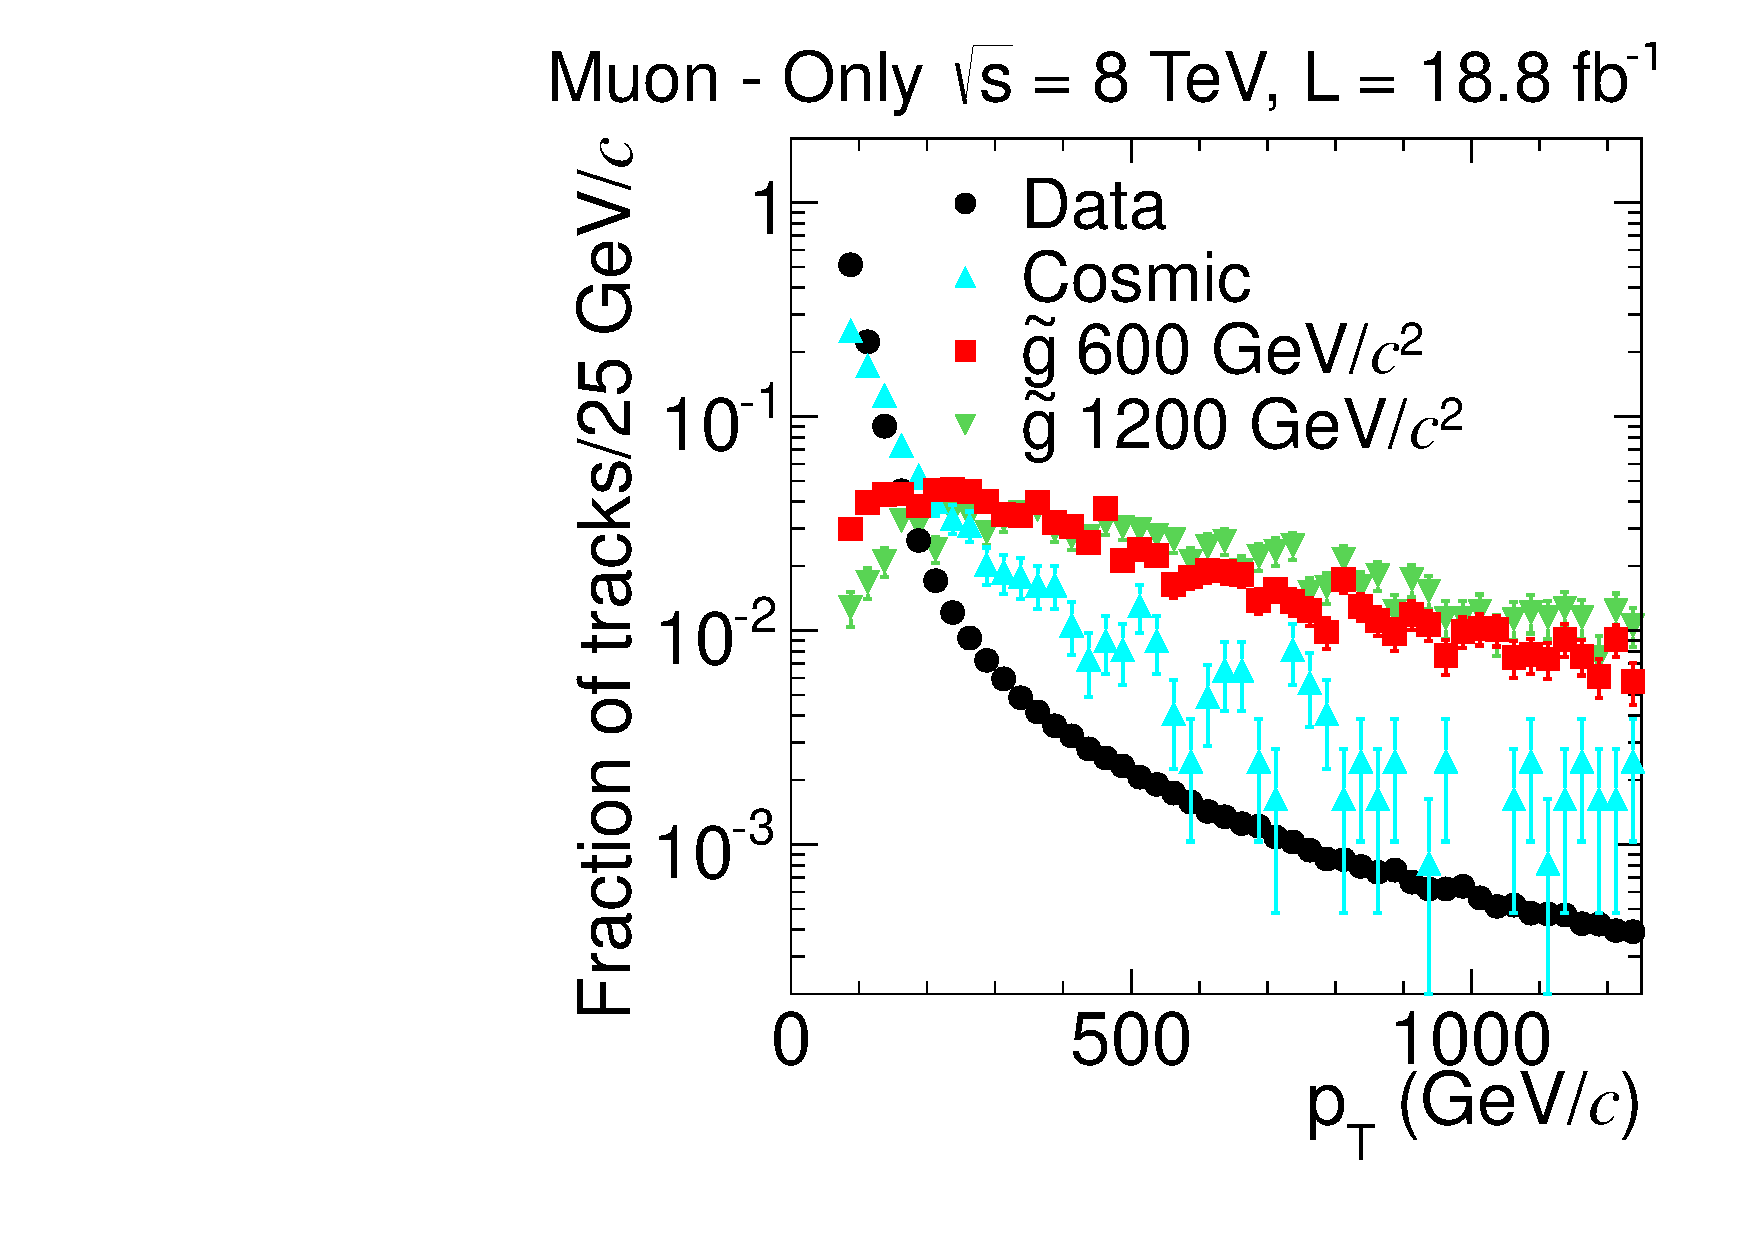
\includegraphics[clip=true, trim=0.0cm 0cm 2.8cm 0cm, width=0.44\textwidth]{figures/muonly/Selection_Comp_8TeV_Cosmic_Pt_BS}
  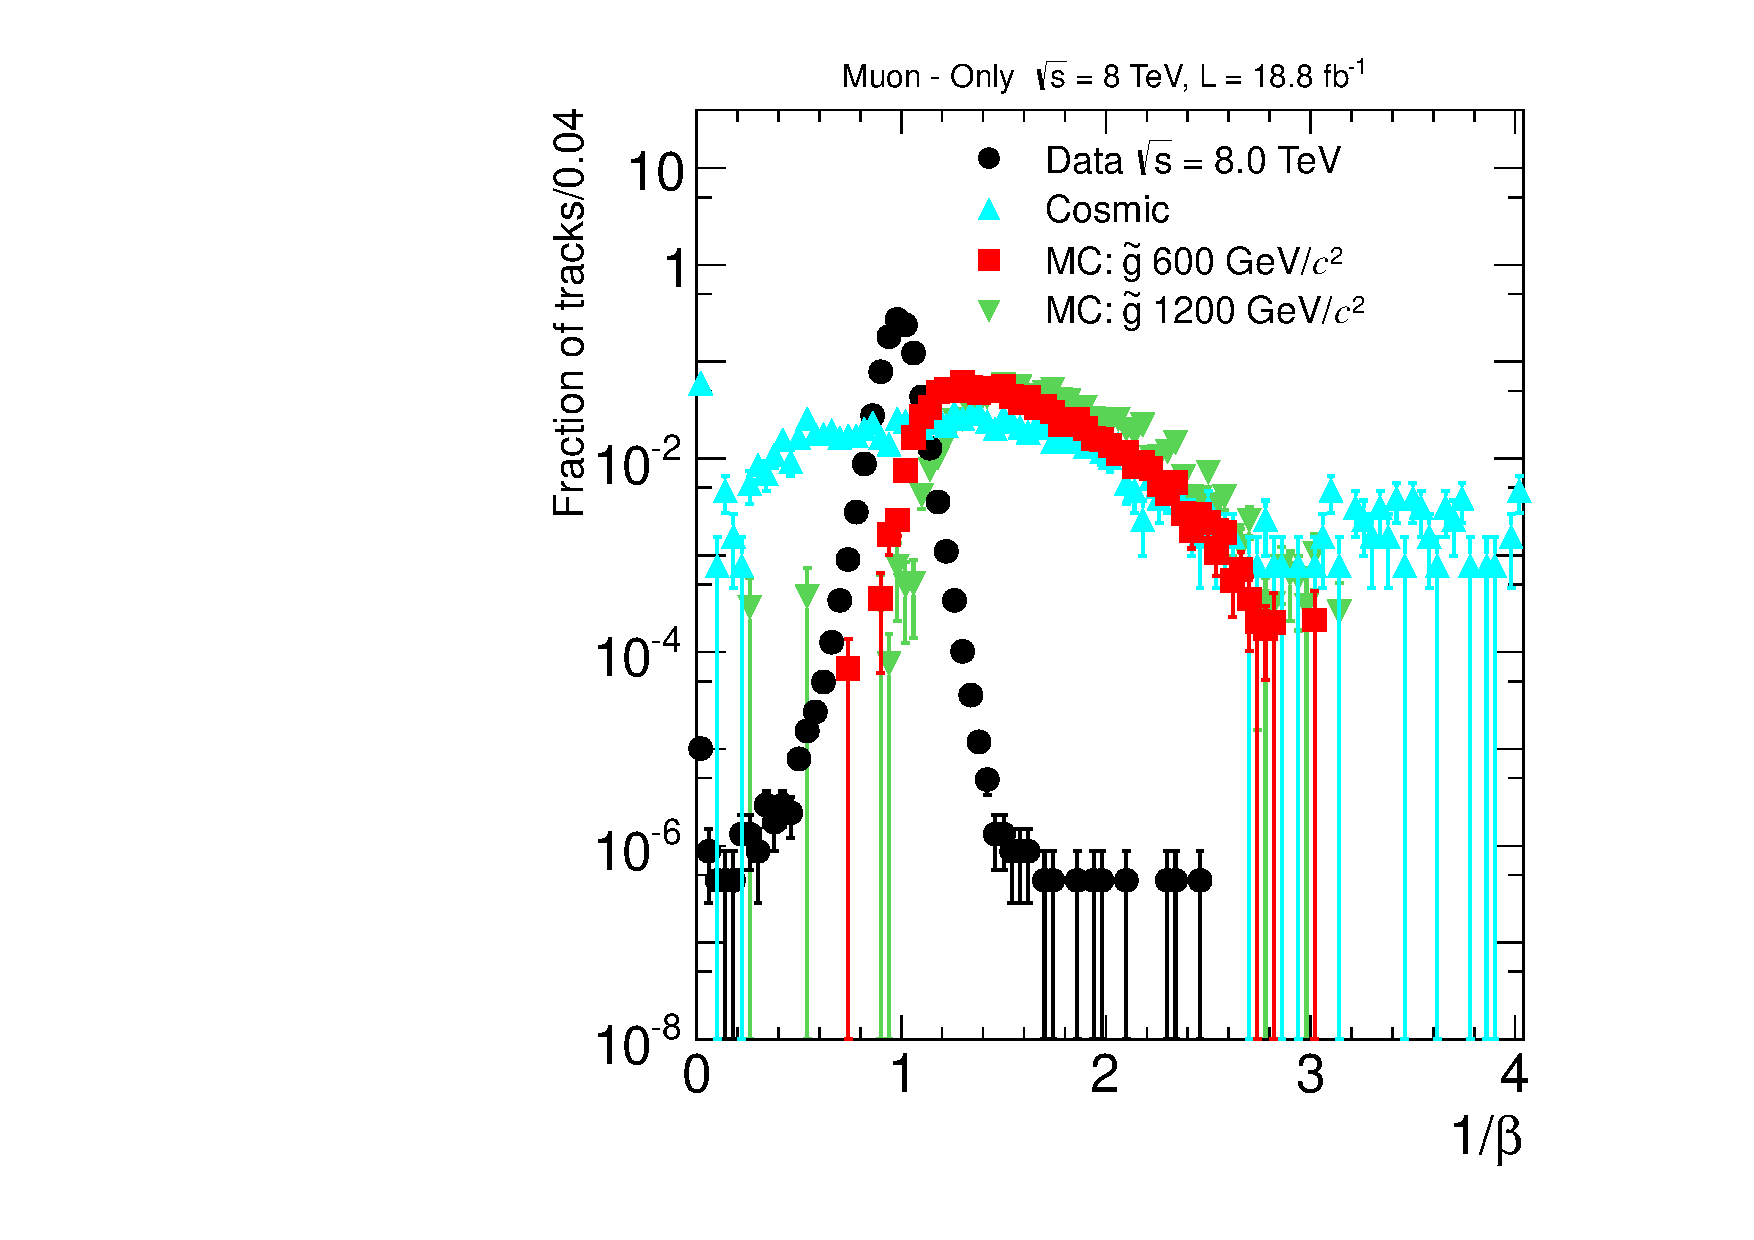
\includegraphics[clip=true, trim=0.0cm 0cm 2.8cm 0cm, width=0.44\textwidth]{figures/muonly/Selection_Comp_8TeV_Cosmic_TOF_BS} \\
  \caption{Distribution of selection variables for data, cosmic control sample, and signal MC.
Left: Distribution of $p_T$. Right: Distribution of \invbeta.
    \label{fig:MuOnlySelVar}}
\end{figure}

\begin{figure}
\centering
  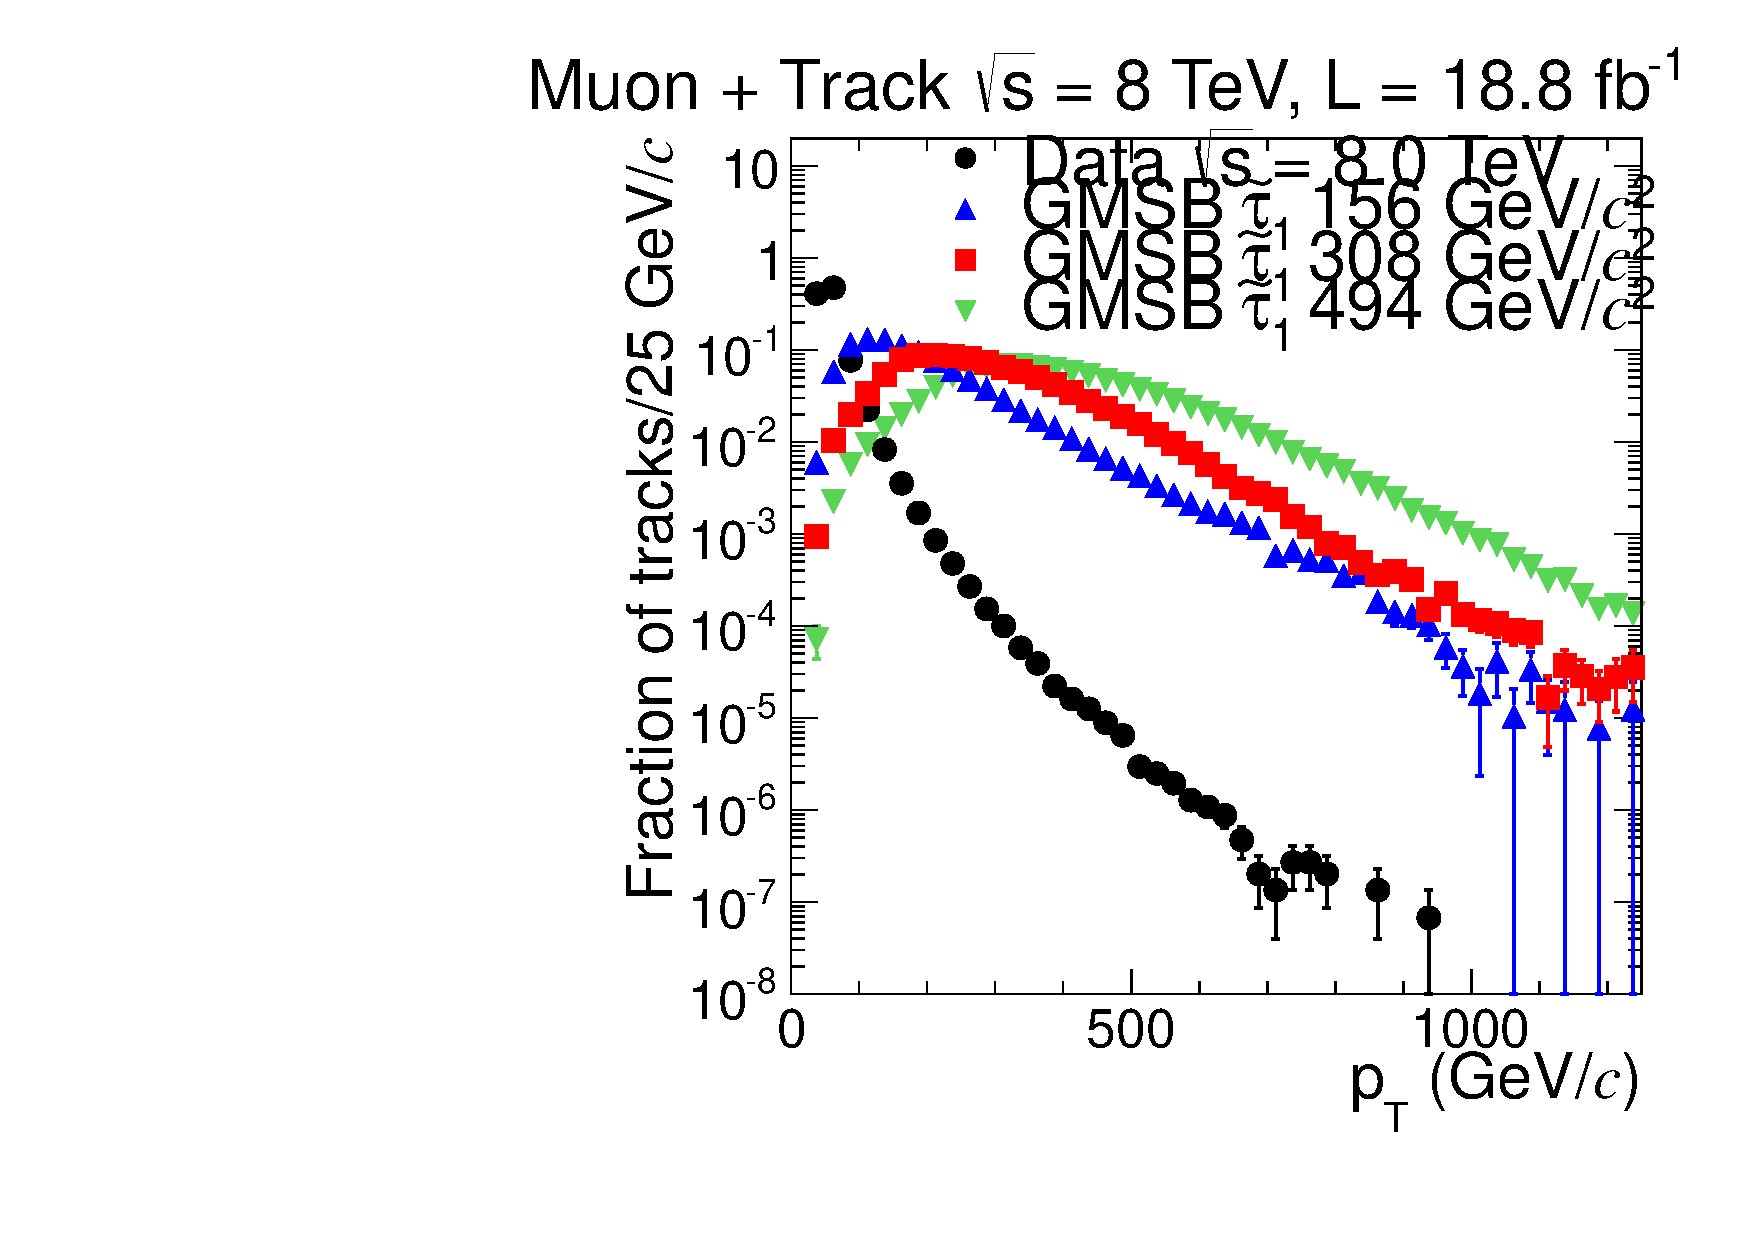
\includegraphics[clip=true, trim=0.0cm 0cm 2.8cm 0cm, width=0.44\textwidth]{figures/tkmu/Selection_Comp_8TeV_GMStau_Pt_BS}
  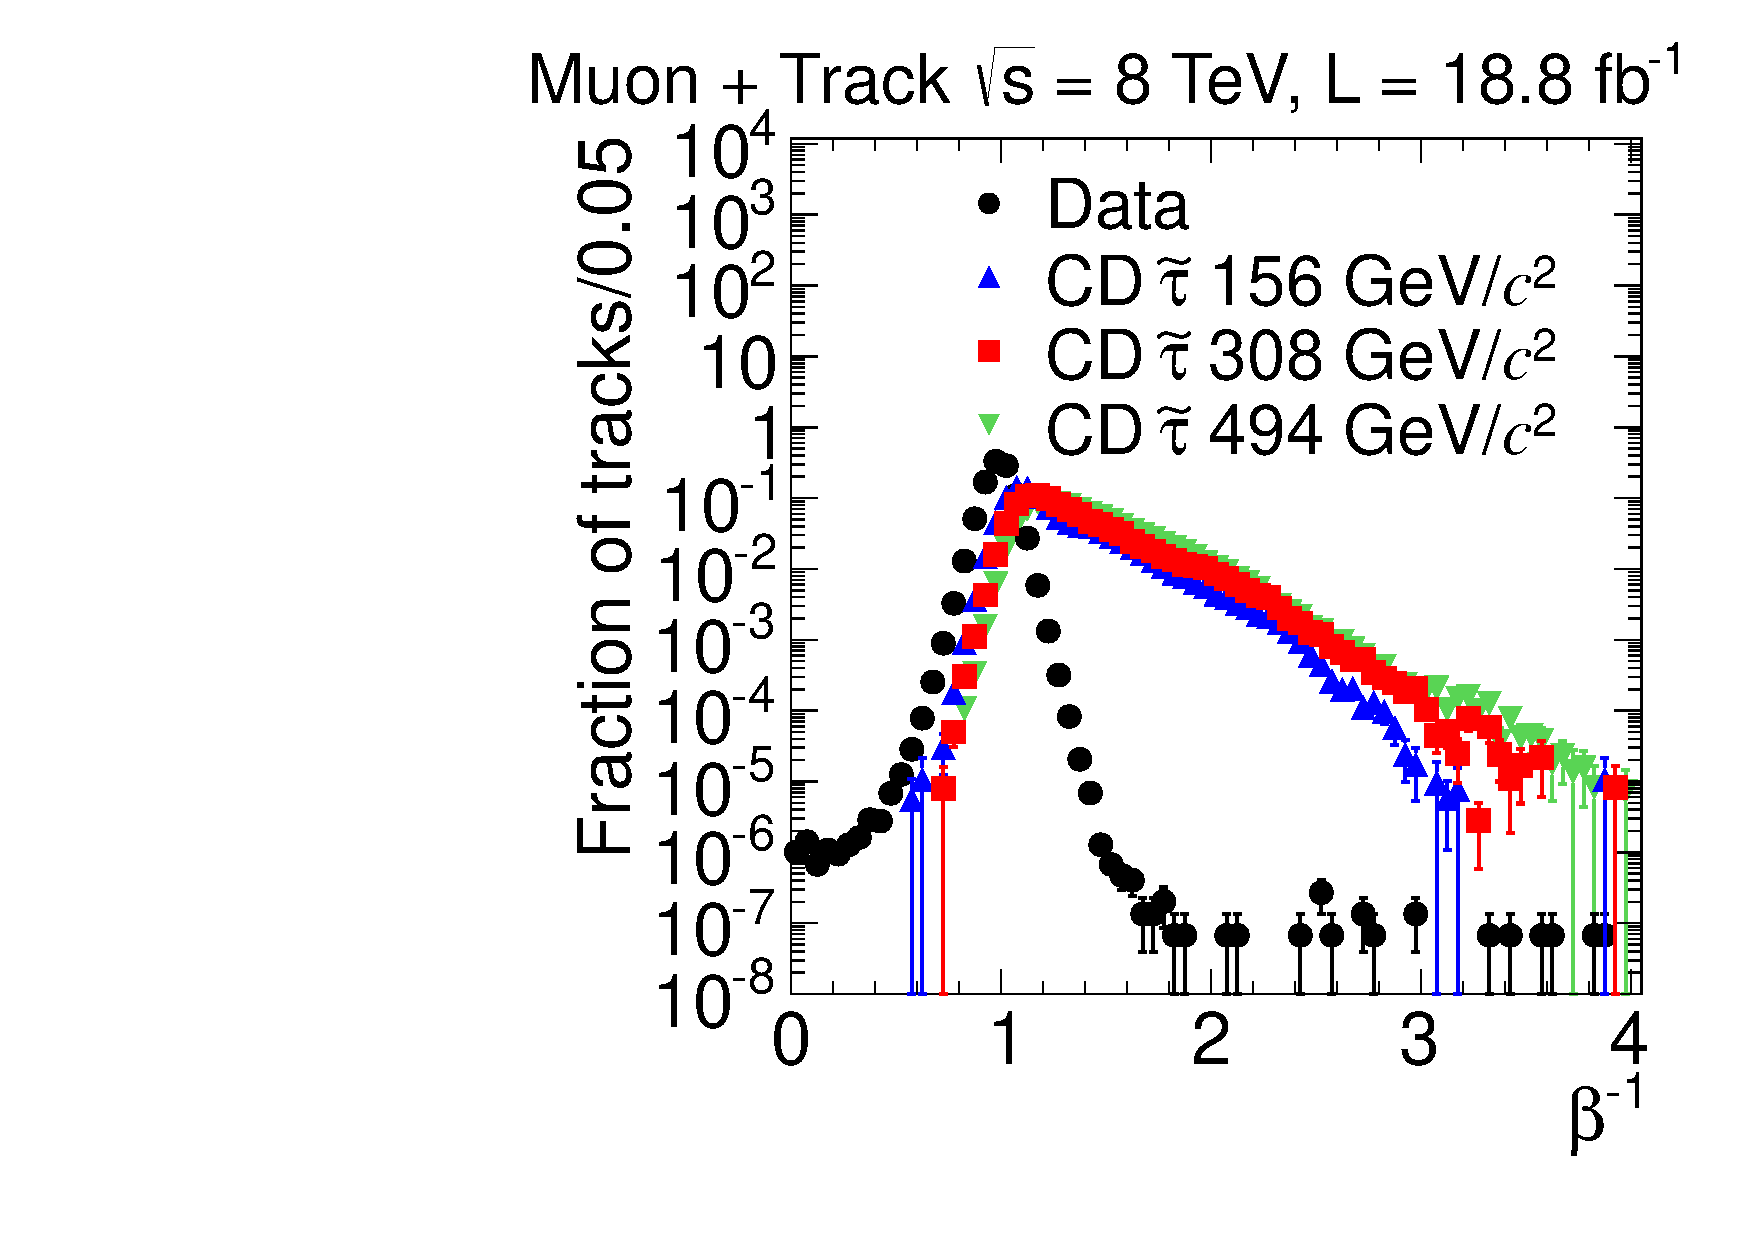
\includegraphics[clip=true, trim=0.0cm 0cm 2.8cm 0cm, width=0.44\textwidth]{figures/tkmu/Selection_Comp_8TeV_GMStau_TOF_BS} \\
  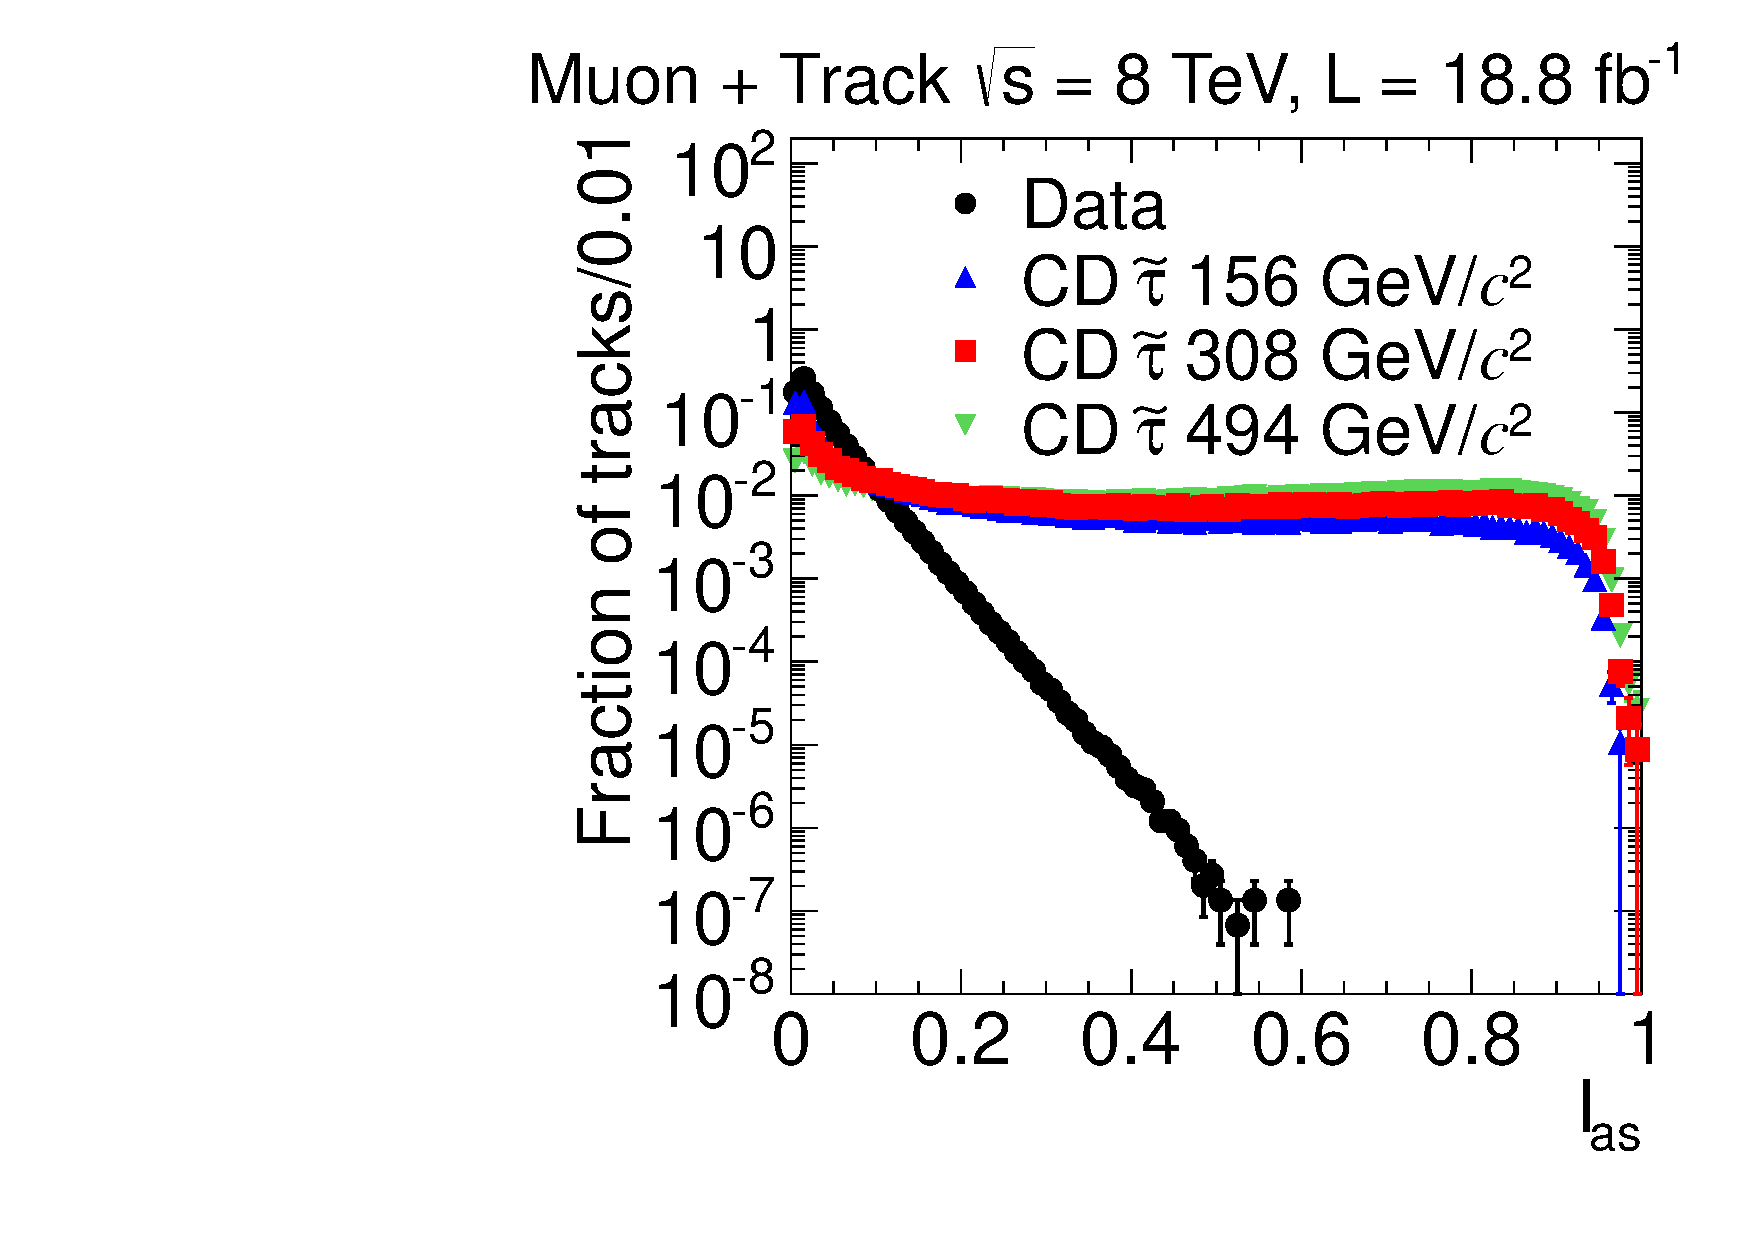
\includegraphics[clip=true, trim=0.0cm 0cm 2.8cm 0cm, width=0.44\textwidth]{figures/tkmu/Selection_Comp_8TeV_GMStau_Is_BS}
  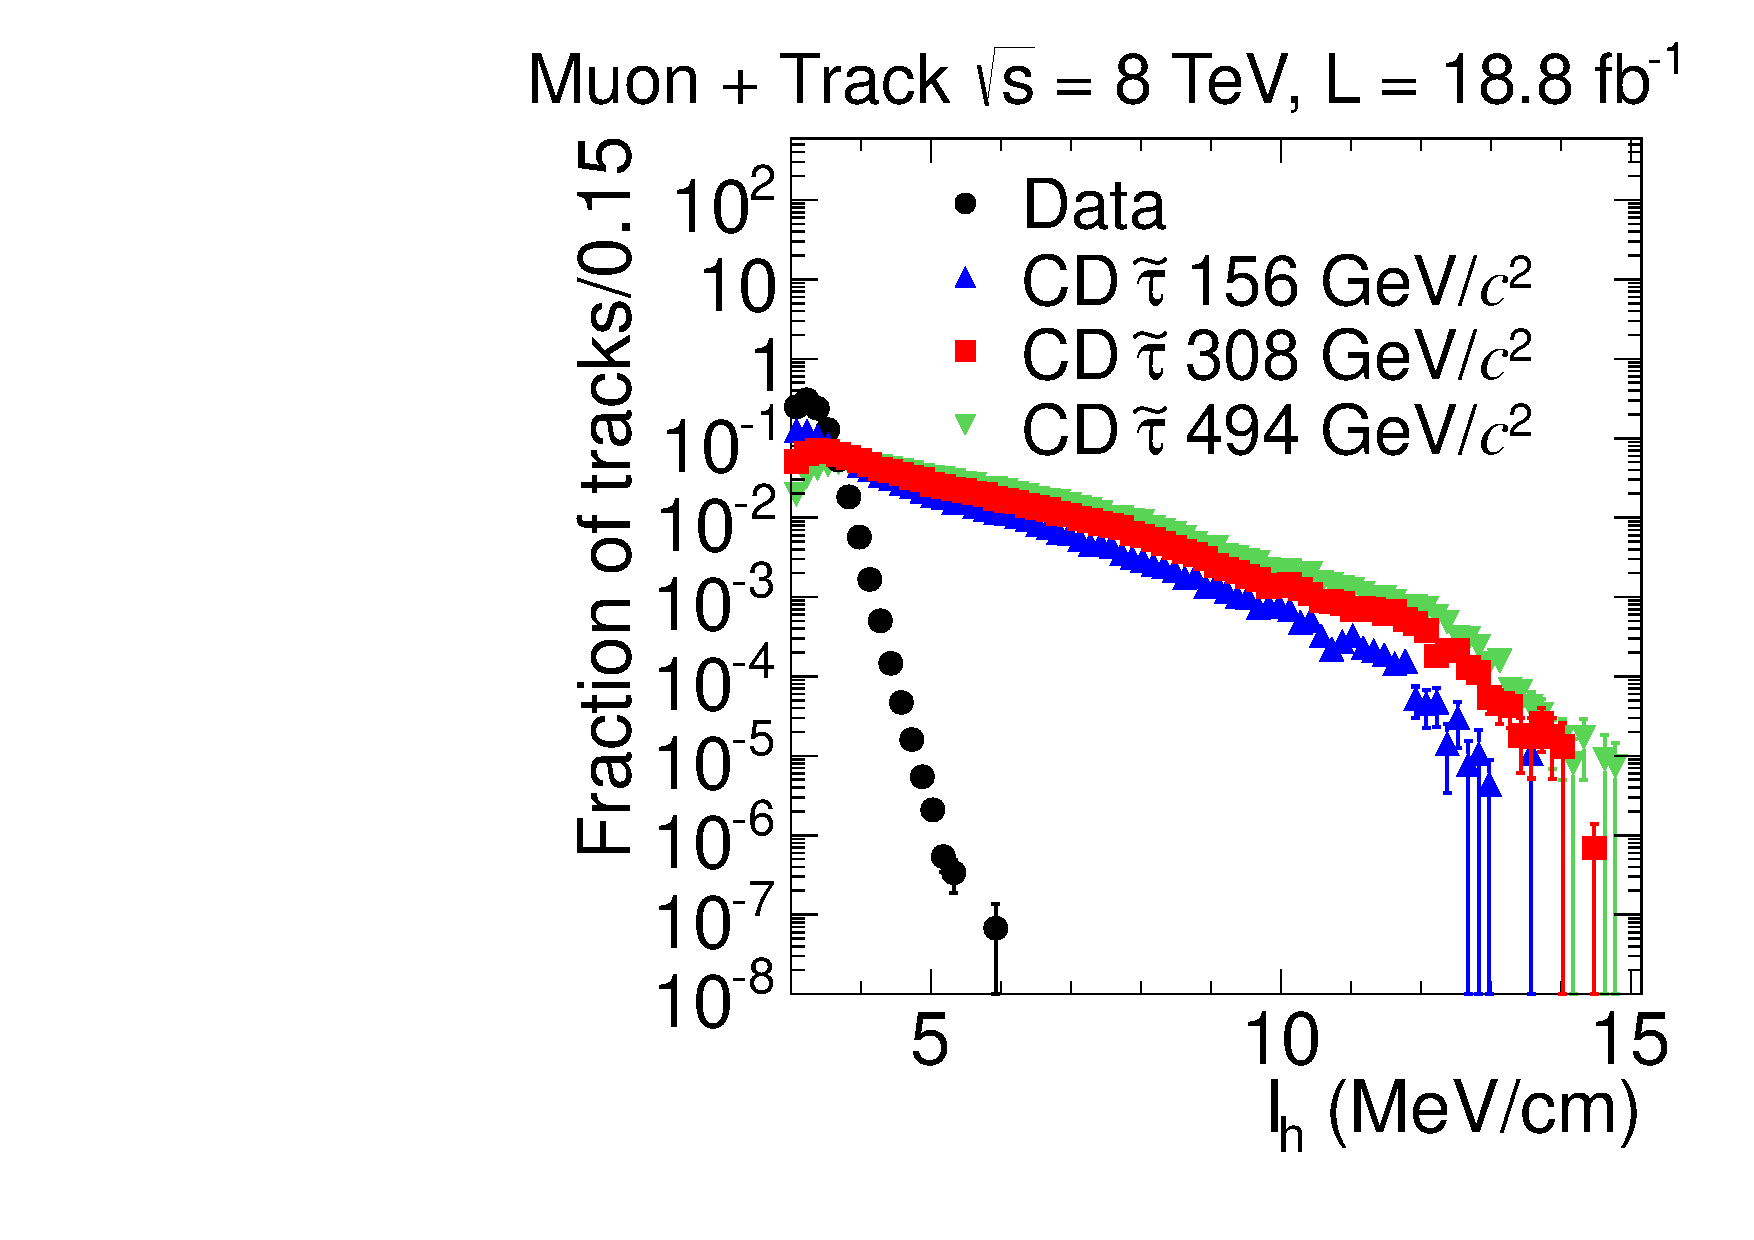
\includegraphics[clip=true, trim=0.0cm 0cm 2.8cm 0cm, width=0.44\textwidth]{figures/tkmu/Selection_Comp_8TeV_GMStau_Im_BS}
  \caption{Distribution of section variables for data and signal MC.
Top row: Distribution of $p_T$ (left) and \invbeta\ (right).
Bottom row: Distribution of \ias\ (left) and \ih\ (right).
    \label{fig:TkMuSelVar}}
\end{figure}

\subsection{Tag and Probe Studies \label{sec:TagProbe}}
The study of the agreement between data and MC for numerous muon qualities is done by the Muon Physics Object Group (POG) inside of CMS.
For all of the analyses except for \muononly\  it is sufficient to use results obtained from this group for possible scale factors between 
data and MC and relevant systematic uncertainties as the variables it selects on are used frequently within CMS.
However, as the \muononly\ analysis uses numerous variables which are unique to the analysis so the values from the muon POG are not applicable.

For this reason additional studies were
performed to test the agreement of MC with data.
The efficiency of the selections was checked with a tag and probe procedure
(from the Muon POG) using muons from the decay of the Z boson. Z bosons decay to a particle and its anti-particle with the invariant mass of the particle--anti-particle
pair equal to the mass of the Z boson they were created from, for the purpose of this study the particles are taken as muons. 

The tag and probe procedure proceeds by
requiring one muon, the tag muon, be found with a very stringent selection trying to assure that this is a good muon. The tag muon is required to pass
a tight selection recommended by the Muon POG and to match to an object that triggered the readout of CMS. The last requirement assures that no bias is
introduced by the need for the event to readout. Additionally the tag must pass the requirements of a skim that was used to reduce the data size to a level
making processing reasonable. The skim requirements were at least three \dedx\ measurements and \ih\ $> 3.0$ or \ih\ $< 2.8$.

Then a set of probe candidates are defined as tracks reconstructed in the inner tracker with no requirement
on muon system activity. The probes are required to have $p_T > 40 GeV$, $|\eta| < 2.1$, and the opposite charge of the tag muon. The invariant mass of the tag and
probe is then required to be within 10 GeV of the mass of the Z boson, 91 GeV.

There are a few processes other than Z boson decay that will lead to tag probe pairs having an invariant mass around the mass of the Z boson. Thus it is likely that the
probe is a muon. This allows to find the efficiency that a muon will pass the preselection in the \muononly\ analysis by looking at the efficiency that the probe
passes the preselection. The efficiencies in data and MC can be compared and any discrepancies accounted for. The residual background from non Z boson decay in the
mass window is accounted for by a fit described below. The MC sample used only contains the creation of Z bosons, background processes are not included.

A simultaneous fit to pairs originating from Z bosons and pairs from background is performed using the
sum of two Voigtians to represent Z bosons and an exponential for the background.
Figure~\ref{fig:MuOnlyTagProbeFit} shows sample fits of
both Data and MC. It can be seen that the fit matches well. The efficiency is extracted from these fits using a procedure from the muon POG.

Figure~\ref{fig:MuOnlyTagProbeEff} shows the efficiency for the probes
to pass the preselection, except for the selection on $p_T$, against the probe
$p_T$, $\eta$, and the number of vertices in the event.
Overall the efficiency is approximately 75\% in data and 80\% in MC.
The efficiency is mostly flat versus $p_T$ and number of vertices but does depend
on $\eta$.  MC is scaled by an $\eta$ dependent amount to correct for the discrepancy.

\begin{figure}
 \begin{center}
  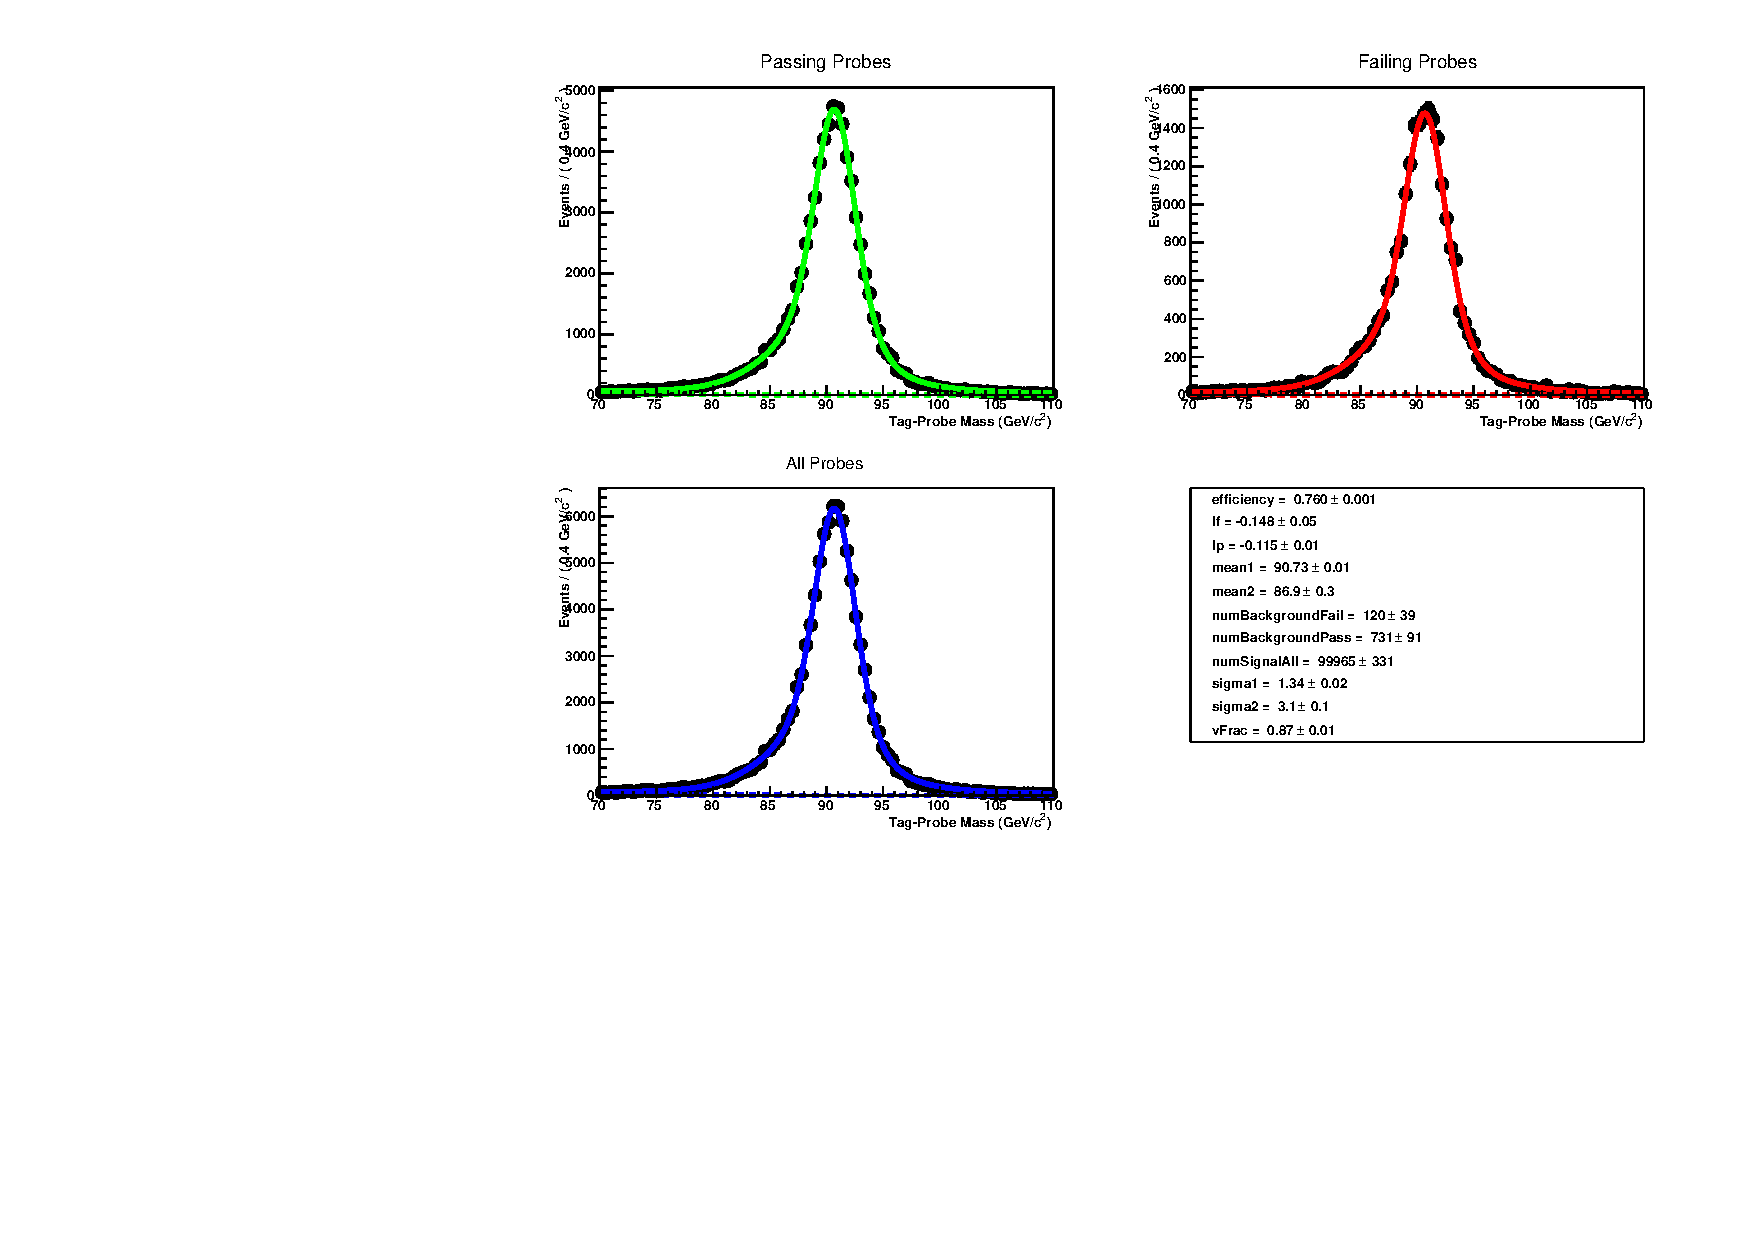
\includegraphics[width=0.95\textwidth]{figures/muonly/FitCanvasDataPtBin0}
 \end{center}
 \caption{Example fit canvas of fit to invariant mass distribution for
the muon efficiency tag and probe measurement for the \muononly\ analysis for data.
    \label{fig:MuOnlyTagProbeFit}}
\end{figure}

\begin{figure}
 \begin{center}
  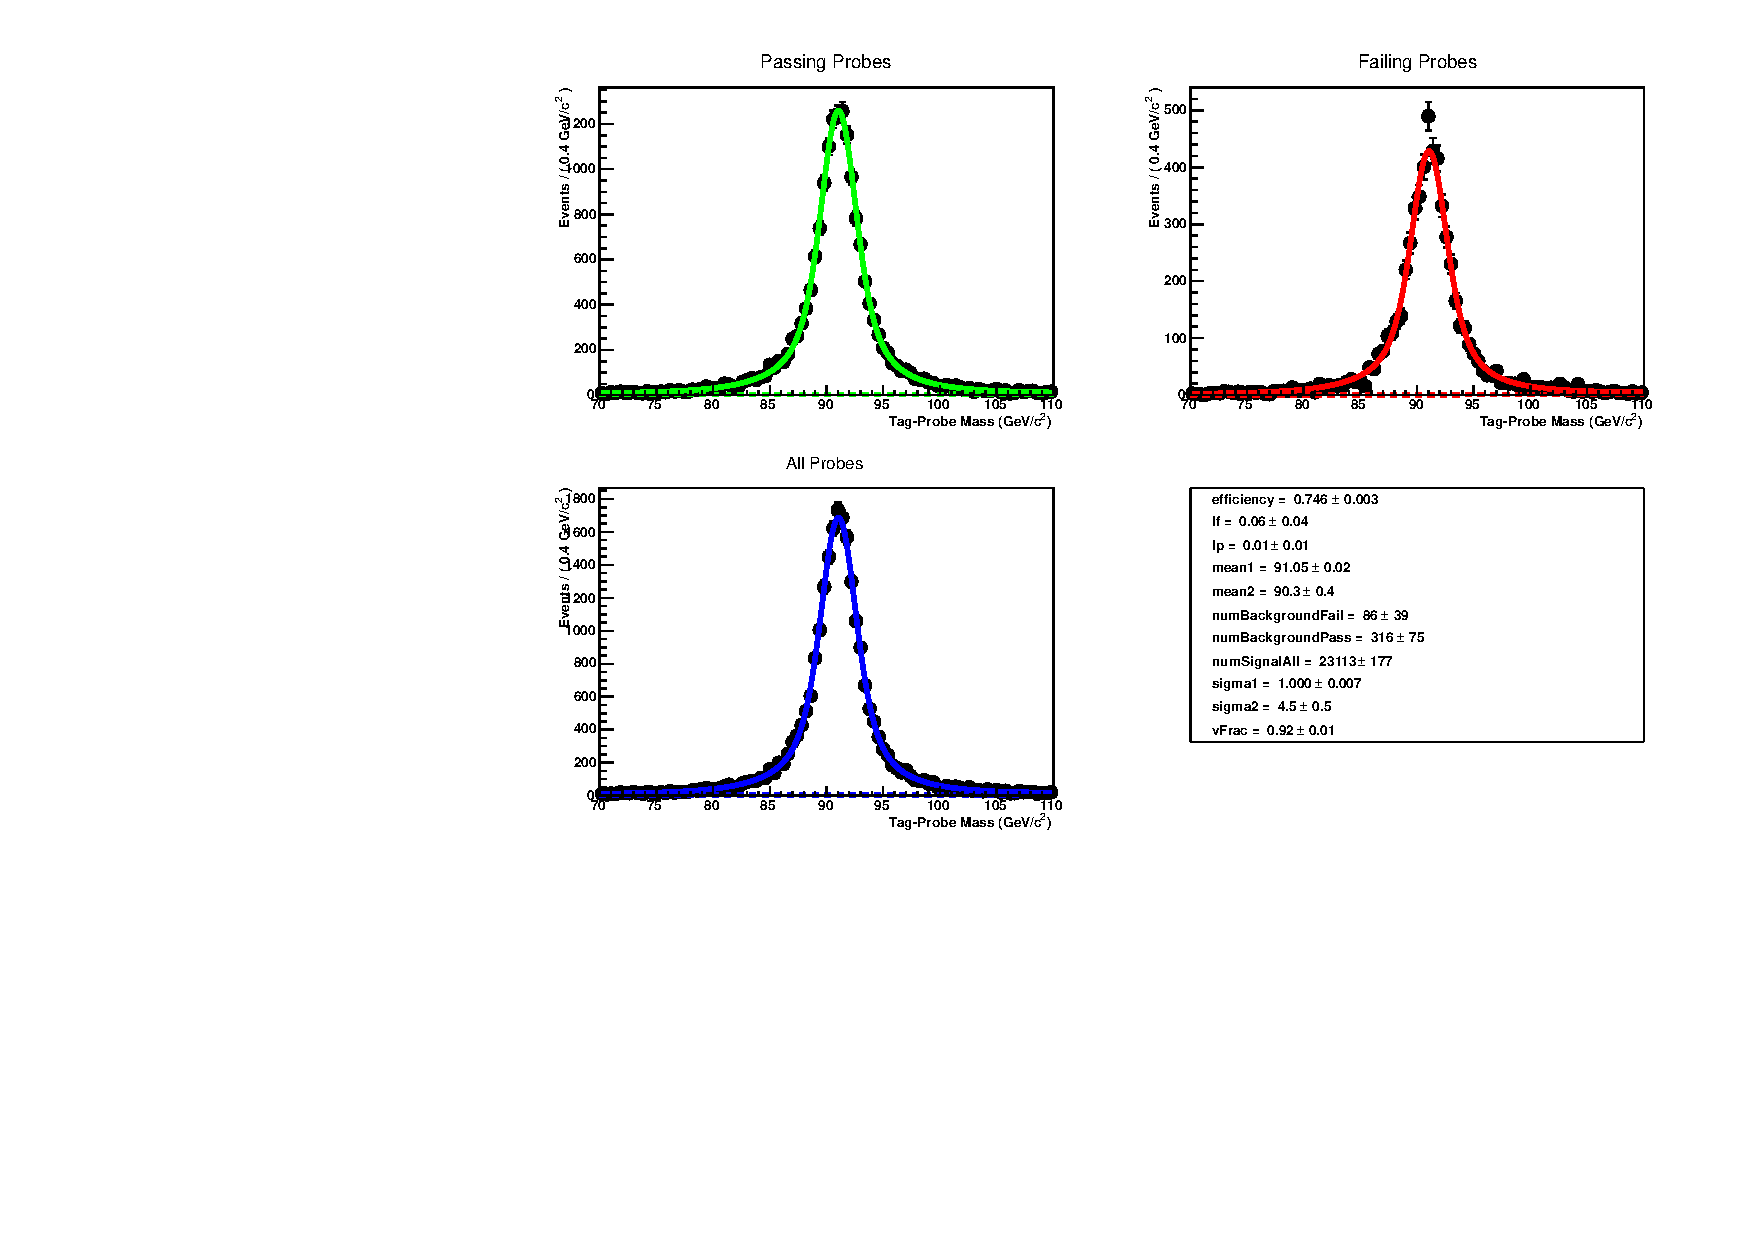
\includegraphics[width=0.95\textwidth]{figures/muonly/FitCanvasMCEtaBin6}
 \end{center}
 \caption{Example fit canvas of fit to invariant mass distribution for
the muon efficiency tag and probe measurement for the \muononly\ analysis for MC.
    \label{fig:MuOnlyTagProbeFit}}
\end{figure}

\begin{figure}
 \begin{center}
  \includegraphics[clip=true, trim=0.0cm 0cm 1.4cm 0cm, width=0.44\textwidth]{figures/muonly/MuonOnlypteff_comp}
  \includegraphics[clip=true, trim=0.0cm 0cm 1.4cm 0cm, width=0.44\textwidth]{figures/muonly/MuonOnlyetaeff_comp}
  \includegraphics[clip=true, trim=0.0cm 0cm 1.4cm 0cm, width=0.44\textwidth]{figures/muonly/MuonOnlyPVeff_comp}
 \end{center}
 \caption{Efficiency to pass preselection cuts for the \muononly\ analysis
   for $p_T$ (left), $\eta$ (center), and number of primary vertices
   (right).
   \label{fig:MuOnlyTagProbeEff}}
\end{figure}

\section{Background Predictions \label{BackPred}}
All of the analyses count the number of tracks passing threshold values on some grouping of the $p_T$, \invbeta, 
and \ias\ variables. The \tktof\  and \tkonly\ analyses also place a requirement on the mass of the track as described below. There are two sources
of background considered in the analyses. 

The first is muons, or for the \tkonly\ analysis any charged SM particle, from the collisions in the LHC. Muons can pass the thresholds on the selection variables
for a variety of reasons.
All muons at the LHC will be traveling at very nearly the speed of light,
but finite detector resolution results in a smearing of the measured time of hits. This can cause muons to have a high measured \invbeta.
While muons in the momentum region of interest all deposit approximately
the same amount of energy in the tracker on average, the amount deposited in each interaction is subject to large variations. This can lead to muons
with a high \dedx\ value. Detector resolution can also contribute to muons with high \dedx.
Additionally, collision muons can have large reconstructed momentum, either due to true high momentum or detector mismeasurement
promoting a low momentum muon to a high reconstructed momentum. Detector mismeasurement is especially important for the momentum measured in the muon system.

Collision muons are predicted by exploiting the lack of correlation between the selection variables for muons through the $ABCD$ method.
In the $ABCD$ method, multiple bins are defined by whether the track passes thresholds on the selection variables. In the normal two dimensional version
of the $ABCD$ method, two selection variables are used and four regions are defined. The $A$ region has tracks failing both of the thresholds on the selection
variables, the $B$ ($C$) region fails only the threshold on the first (second) of the selection variables, and the $D$ region,
the signal region, passes the threshold on both selection
variables. The number of background muons in the $D$ region can be predicted as $B \times C / A$, where the letters represent the number of tracks in the regions.
This prediction holds as long as the probability for a background
muon to pass the threshold on one of the variables is independent of whether it passes the threshold of the other. Tests of the correlation between the selection variables are
given below.

The four different analyses use different combinations of the selection variables defined in Sec.~\ref{sec:SelVar}. 
With three different selection variables (\pt, \invbeta, \dedx), eight different bins are defined.
In order to simplify the nomenclature in this section, Table~\ref{tab:BinNames} 
defines the names of the bins (ranging from $A$-$H$) and whether they pass or fail the thresholds on the selection variables. For all
the selection variables passing means having a value above the threshold. If a selection variable
is not used in an analysis then it is taken to have passed. 

Only the \tktof\ analysis applies a threshold on all three selection variables and as such is the only one to use all eight bins.
An extended three-dimensional version of the $ABCD$ method is then used to make the prediction as is described in the \tktof\ subsection below.
The other three analyses use only the four bins where the unused variable is said to have passed. These analyses use the traditional two-dimensional $ABCD$ method
though the names of the bins may be different.
For all the analyses the D region is always the signal region. 

In order to perform systematic studies, the analyses that use \invbeta\ reverse the preselection requirement on \invbeta\ greater than one. This creates a group of tracks
measured as going faster than the speed of light, making it signal free. As the \invbeta\ distribution is close to symmetrical for background muons,
this region is very good for testing the background prediction. New bins are defined as in Table~\ref{tab:BinNames} but now \invbeta\ is said to have passed
if the value is below the threshold. The bins are referred to with a prime to denote that they are from the control region, so the new ``signal'' region would
be referred to as $D^{\prime}$.


\begin{table}
 \begin{center}
  \caption[Bin naming convention for background regions]
{Bin naming convention.  The signal region is always the D region.}
     \label{tab:BinNames}
  \begin{tabular}{|c|c|c|c|} \hline
   Name & $p_T$ & \invbeta\   & \dedx\  \\ \hline
   A    & Fail      & Fail            & Pass           \\ \hline
   B    & Fail      & Pass            & Pass           \\ \hline
   C    & Pass      & Fail            & Pass           \\ \hline
   D    & Pass      & Pass            & Pass           \\ \hline
   E    & Fail      & Fail            & Fail           \\ \hline
   F    & Fail      & Pass            & Fail           \\ \hline
   G    & Pass      & Fail            & Fail           \\ \hline
   H    & Pass      & Pass            & Fail           \\ \hline
  \end{tabular}
 \end{center}
\end{table}

The second source of background, important only for the \muononly\  analysis,
%and \fract\ analyses, 
is muons from cosmic-rays. 
As discussed in Section~\ref{sec:SM} muons from cosmic-rays
are constantly passing through CMS. Cosmic-ray muons will arrive to the muon system asynchronously with collisions in the LHC. Depending on exactly
when the cosmic-ray muon arrives in the muon system relative to collisions in the LHC this can give rise to a particle with a large \invbeta\ measurement.
The distribution of $p_T$ for cosmic-ray muons falls off at high momentum slower than for collision muons, as evidenced in Figure~\ref{fig:MuOnlySelVar} (left).
As cosmic-ray muons have different \invbeta and \pt\ distributions than collision muons they will not be accurately predicted with the same method used to predict
the collision-muon background in the \muononly\ analysis. A dedicated method using the cosmic-ray muon control sample is described below.

Cosmic-ray muons are not considered for the analyses that look for high-ionizing tracks as
out-of-time particles are not centered in the tracker's charge collection window.
This results in only a portion of their ionization energy loss being collected and their reconstructed \dedx\ being smaller than a collision muon.
Thus, cosmics have the signature of anomalously low reconstructed \dedx~\cite{CMS:2012xi} opposite of the signature for an HSCP.
%This combined with the impact parameter requirements applied at preselection makes cosmic-ray muons negligible for the analyses looking for high \dedx\ in the tracker.

For all the analyses, the expected background in the signal region is estimated by multiple different predictions.
The details on how the different predictions are found for each analysis are given in the corresponding subsection below.
The spread of the different background predictions can be used to estimate the systematic uncertainty for each analysis.

The following variables are defined:
\begin{equation}
\centering
\begin{split}
S^{syst+stat}_{N} &= \sqrt{\sum_i \left( x_i - \langle x \rangle  \right) ^2/(N-1)} \\
S^{stat}_{N} &= \sqrt{\sum_i \left( \sigma _i \right) ^2/N} \\
S^{syst} &= \sqrt{S_{syst+stat}^2-S_{stat}^2} \\
\end{split}
\label{eq:variance}
\end{equation}
where N is the number of background estimates made,
the sum is over N, $x_i$ is the value of the $i^{th}$ background estimate,
and $\sigma_i$ is the statistical uncertainty on
the $i^{th}$ background estimate. The first quantity is an estimator of the
standard deviation of the background estimates, which takes both statistical
and systematic contributions. The second quantity is adopted as an
estimator of the contribution of the statistical uncertainties
to the standard deviation. Finally, the last equation gives the systematic uncertainty on the background prediction assuming
the statistical and systematic uncertainties add in quadrature to give the standard deviation.

\subsection{Prediction for \muononly\ analysis \label{sec:MuOnlyPred}}

The collision muon  background in the \muononly\ analysis is predicted with the selection criteria of \invbeta\ and \pt\ in the $ABCD$  method.
%by exploiting the lack of correlation between the selection variables for background particles. 
The expected number of background tracks in the signal region $D$ (see Table~\ref{tab:BinNames}) is predicted as $B \times C / A$. 
%Tracks are divided into four groups based on whether they
%have $p_T$ and \invbeta\ values greater than the thresholds placed on these selection criteria. 
%The four groups are referred to as $A$,$B$,$C$, and $D$. The $A$ group contains tracks that have $p_T$ and \invbeta\ values lower than both selection thresholds
%while the $B$($C$) group contains tracks that have only the $p_T$ (\invbeta) below its threshold. The groups containing the tracks with \invbeta\
%below the its threshold only contains tracks with $1 < $\invbeta\ $< $ threshold. Tracks with \invbeta\ $< 1$ are used to evaluate how well the prediction performs.
%The $D$ group contains tracks passing both thresholds and is considered the signal region. 

%The predicted number of collision muons in the signal region is found via the relation $B \times C / A$. This relation is accurate so long as the ratio of tracks
%passing the \invbeta\ cut is the same regardless of whether the $p_T$ cut is passed, the statement is also true reversing the roles of \invbeta\ and $p_T$.
The $ABCD$ method only works if the probability to pass one of the thresholds is independent of the other variable.
However, it has been observed that a correlation exists between the $p_T$ and \invbeta\ measurements based on whether the track is in the barrel or forward
region of the detector as well as the number of DT or CSC stations containing valid hits. 
Six bins are created defined by the $\eta$ of the track, greater or less than 0.9; and the number of stations, 2, 3, or 4.
The distributions of \pt\ and \invbeta\ in the six regions is shown in Figure~\ref{fig:SelVarBinned}.
The predicted number of tracks in each bin is predicted separately and the total number of predicted background tracks is the sum of the six predictions.

\begin{figure}
\centering
  \includegraphics[clip=false, trim=0.0cm 0cm 0.0cm 0cm, width=0.48\textwidth]{figures/muonly/Selection_Data8TeV_Pt_Binned_BS}
  \includegraphics[clip=false, trim=0.0cm 0cm 0.0cm 0cm, width=0.48\textwidth]{figures/muonly/Selection_Data8TeV_TOF_Binned_BS}
\caption[Distribution of $p_T$ and \invbeta\ for data in different prediction regions in the \muononly\ analysis]
{Distribution of $p_T$ and \invbeta\ for data for six different regions depending on whether the track is in the barrel (Bar)
or forward (For) region of CMS and number of muon stations (Sta) used in the fit.}
    \label{fig:SelVarBinned}
\end{figure}

After the binning the correlation is small enough not to bias the background prediction as can be seen in Figs.~\ref{fig:MuOnlyControl} and~\ref{fig:MuOnlyControl4}.

\begin{figure}
\begin{center}
\includegraphics[clip=false, trim=0.0cm 0cm 0.0cm 0cm, width=0.48\textwidth]{figures/muonly/Control_Data8TeV_Pt_TOFSpectrum_Binned_0}
\includegraphics[clip=false, trim=0.0cm 0cm 0.0cm 0cm, width=0.48\textwidth]{figures/muonly/Control_Data8TeV_Pt_TOFSpectrum_Binned_3} \\
\includegraphics[clip=false, trim=0.0cm 0cm 0.0cm 0cm, width=0.48\textwidth]{figures/muonly/Control_Data8TeV_Pt_TOFSpectrum_Binned_1}
\includegraphics[clip=false, trim=0.0cm 0cm 0.0cm 0cm, width=0.48\textwidth]{figures/muonly/Control_Data8TeV_Pt_TOFSpectrum_Binned_4}
\caption[Distribution of \invbeta\
for different momentum regions for two and three station tracks in the \muononly\ analysis.]
{Distribution of \invbeta\ 
for different momentum regions for four of the six different bins that are used to make the prediction.
The left column shows the barrel region while the right column
shows the forward region.  The top (bottom) row are for 2 (3) stations.}
\label{fig:MuOnlyControl}
\end{center}
\end{figure}

\begin{figure}
\begin{center}
\includegraphics[clip=false, trim=0.0cm 0cm 0.0cm 0cm, width=0.48\textwidth]{figures/muonly/Control_Data8TeV_Pt_TOFSpectrum_Binned_2}
\includegraphics[clip=false, trim=0.0cm 0cm 0.0cm 0cm, width=0.48\textwidth]{figures/muonly/Control_Data8TeV_Pt_TOFSpectrum_Binned_5}
\caption[Distribution of \invbeta\
  for different momentum regions for four station tracks in the \muononly\ analysis.]
{Distribution of \invbeta\
for different momentum regions for four station tracks.
The  left column shows the barrel region while the right column
shows the forward region.}
\label{fig:MuOnlyControl4}
\end{center}
\end{figure}

To predict the cosmic-ray-muon background, sidebands in the $|\delta_z|$ distribution and the pure cosmic-ray muon sample (see Section~\ref{sec:samples}) are used.
The number of tracks, $N$, in a sideband region of $|\delta_z|$ are counted. The tracks are required to pass the full selection except the $|\delta_z|$ requirement 
is changed from $0 < |\delta_z| <$~15~cm to $70 < |\delta_z| <$~120~cm and
the requirements on $\phi,$ segment $\eta$ separation, and $p_T$ are removed to increase the number of cosmic-ray muons in the sideband region. 
Additionally the tracks
are required not to be reconstructed in the silicon tracker to decrease the contamination from collision muons. 
Then, the pure cosmic-ray sample is used to calculate the ratio, $R$, of tracks in the $|\delta_z|$ sideband region 
relative to the signal region with the same offline requirements as in the main data sample. 

The number of cosmic-ray muons passing the final selection in the main data sample can then be predicted as 
\begin{equation}
\begin{split}
P_{Cosmic} = N \times R.
\end{split}
\label{eq:CosmicPred}
\end{equation}
Numerous effects cancel in this ratio making the prediction robust. The number of cosmic-ray muons in any of the regions can be expressed as 
$C = F \times T \times \epsilon$, where C is the number of cosmic-ray muons observed, F is the flux of cosmic-ray muons per second, T is the amount of time that CMS was collecting data, and $\epsilon$ is the efficiency of the detector to reconstruct and select cosmic-ray muons in the region including detector acceptance effects. 

The number of cosmic-ray muons expected in the signal region can be written as
\begin{equation}
\begin{split}
P_{Cosmic} = F \times T_{Main} \times \epsilon_{Main}^{Signal}
\end{split}
\label{eq:CosmicSignal}
\end{equation}
and the number N in the sideband region as 
\begin{equation}
\begin{split}
N = F \times T_{Main} \times \epsilon_{Main}^{Sideband}
\end{split}
\label{eq:CosmicSide}
\end{equation}
with Main referring to the samples gathered with the main analysis triggers
and Signal and Sideband representing the $|d_z|$ signal and sideband regions, respectively.
The ratio R can be expressed as
\begin{equation}
\begin{split}
R = F \times T_{Control} \times \epsilon_{Control}^{Signal} / (F \times T_{Control} \times \epsilon_{Control}^{Sideband}) = \epsilon_{Control}^{Signal} / \epsilon_{Control}^{Sideband}\\
\end{split}
\label{eq:CosmicRatio}
\end{equation}
where Control refers to the pure cosmic-ray muon control sample.

Putting this all together and canceling numerous factors, it can be seen that Eq.~\ref{eq:CosmicPred} holds so long as the relationship
%\begin{equation}
%\begin{split}
%& F \times T_{Main} \times \epsilon_{Main}^{Signal} = F \times T_{Main} \times \epsilon_{Main}^{Sideband} \times \epsilon_{Control}^{Signal} / \epsilon_{Control}^{Sideband} \\
%\end{split}
%\label{eq:CosmicDetail}
%\end{equation}
%where Main and Control differentiate between the main triggers used in the analysis from the cosmic control trigger, respectively,
% and signal and sideband represent the signal region and $|d_z|$ sideband, respectively. 
%After the cancellation of numerous factors this equation reduces to 

%\begin{equation}
%\epsilon_{Main}^{Signal} = \epsilon_{Main}^{Sideband} \times \epsilon_{Control}^{Signal} / \epsilon_{Control}^{Sideband}
%\label{eq:ReducedCosmicPred}
%\end{equation}
%It is clear that as long as the relationship
\begin{equation}
\epsilon_{Main}^{Signal}/ \epsilon_{Main}^{Sideband} = \epsilon_{Control}^{Signal} / \epsilon_{Control}^{Sideband}
\label{eq:ReducedCosmicPredRatio}
\end{equation}
is accurate. The only difference between the two ratios is that one is using events collected with the main triggers while the
other is using the cosmic-ray muon control trigger. As the offline requirements on tracks reinforce the trigger selection,
the two samples are very similar.
Thus the prediction of the number of cosmic-ray muons in the signal region should be robust. Note that the relationship does not require the efficiency
in the cosmic-ray muon control sample to be the same as in the main sample. Only that the ratio of the efficiencies in the signal and sideband regions
be the same in the two samples.

As previously mentioned, the background prediction is checked using tracks with \invbeta\ less than one. This region is useful as it is background dominated
and provides a good approximation of background tracks in the signal region as the \invbeta\ distribution is roughly symmetrical about one for background tracks.
The background prediction procedure described above is repeated but instead looking for high \pt\ tracks with \invbeta\ below some threshold.
This is the same procedure that would be taken to look for particles that travel faster than the speed of light.
As described above, the bins in the low \invbeta\ region are given a prime so the new ``signal'' region is labelled $D^{\prime}$.
% can be predicted as
%$C^{\prime} \times B^{\prime}/A^{\prime}$. 
Figure~\ref{fig:PredFlipPt230} shows the number of predicted and observed tracks in $D^{\prime}$ for different $p_T$
and \invbeta\ thresholds. The predicted number of tracks includes the prediction for both collision muons and cosmic-ray muons.
Good agreement is seen between the observed and predicted number of tracks. 

\begin{figure}
\centering
  \includegraphics[clip=false, trim=0.0cm 0cm 0.0cm 0cm, width=0.48\textwidth]{figures/muonly/Prediction_Data8TeV_NPredVsNObs_Flip}
  \caption[Number of predicted and observed tracks in the \invbeta\ $<$ 1 region in the \muononly\ analysis]
{Number of predicted and observed tracks passing thresholds on \pt\ and \invbeta. The tracks are required to be above the \pt\ threshold and below the \invbeta\ threshold.
Two representative $p_T$ thresholds are shown. Threshold for \invbeta\ set by x-axis.
Figure is cumulative as tracks passing the selection with tight thresholds will also pass for loose thresholds.}
    \label{fig:PredFlipPt230}
\end{figure}

To determine the systematic uncertainty on the predicted collision background, the \invbeta\ less than one region is used once again. The predicted number of tracks
in the signal region D can be predicted by three different formulae, the main one of $B \times C/A$ as well as 
$B \times C^{\prime}/A^{\prime}$ and $B \times D^{\prime}/B^{\prime}$. The $B$ region contains tracks with \invbeta\ above the final selection threshold and
\pt\ below its threshold. The ratios $C/A$, $C^{\prime}/A^{\prime}$, and $D^{\prime}/B^{\prime}$ give the fraction of tracks to be above the threshold on \pt\
in the region with \invbeta\ between one and the final threshold; the region with \invbeta\ between a value less than one, for example 0.8, and one;
and the region with \invbeta\ below
the same less than one value, respectively. Thus the different predictions can be used to evaluate how the fraction of background tracks to pass the \pt\ threshold depends on
their \invbeta.
%The first of the additional predictions would be sensitive to any shift in the \invbeta\ distribution due to the $p_T$ requirement while the second would be
%sensitive to any effect on the resolution due to the $p_T$ requirement. 
Figure~\ref{fig:MuOnlycorrelation} shows the number of predicted tracks from the three predictions for different \invbeta\ and $p_T$ thresholds.

\begin{figure}
\begin{center}
\includegraphics[clip=false, trim=0.0cm 0cm 0.0cm 0cm, width=0.48\textwidth]{figures/muonly/Data8TeVCollisionPrediction_TOF110}
\includegraphics[clip=false, trim=0.0cm 0cm 0.0cm 0cm, width=0.48\textwidth]{figures/muonly/Data8TeVCollisionPrediction_TOF120}
\caption[Distributions of the number of predicted tracks with different prediction formulae for different sets of thresholds in the \muononly\ analysis.]
{Distributions of the number of predicted tracks and their statistical uncertainty with different prediction formulae for different sets of thresholds.
The $p_{T}$ threshold is defined by the x-axis.
Figures are cumulative as tracks passing the selection with tight thresholds will also pass for loose thresholds.
Left: $1/\beta>1.1$ ($<0.9$ for low $1/\beta$ regions). Right: $1/\beta>1.2$ ($<0.8$ for low $1/\beta$ regions).}
\label{fig:MuOnlycorrelation}
\end{center}
\end{figure}

The systematic uncertainty is extracted from the three predictions
through Eq.~\ref{eq:variance} with N=3.
Fig.~\ref{fig:MuOnlyUnc} shows the variation of
$S_{syst+stat}/\langle x \rangle $, $S_{stat}/ \langle x \rangle $ and $S_{syst}/ \langle x \rangle $
as a function of the $p_T$ threshold. The statistical uncertainty due to the number of tracks in the $B$ group is not subtracted as it is completely correlated
between the three predictions. From the last plot
the systematic uncertainty on the expected background in the signal
region is estimated to be 20\%.

\begin{figure}
\begin{center}
\includegraphics[clip=false, trim=0.0cm 0cm 0.0cm 0cm, width=0.48\textwidth]{figures/muonly/Data8TeVCollisionStat}
\includegraphics[clip=false, trim=0.0cm 0cm 0.0cm 0cm, width=0.48\textwidth]{figures/muonly/Data8TeVCollisionStatSyst} \\
\includegraphics[clip=false, trim=0.0cm 0cm 0.0cm 0cm, width=0.48\textwidth]{figures/muonly/Data8TeVCollisionSyst}
\caption[Statistical and systematic uncertainties in the background prediction for different sets of thresholds in the \muononly\ analysis.]
{Relative uncertainty on the collision-muon background prediction in the \muononly\ analysis.
Two different \invbeta\ thresholds are plotted. Threshold on \pt\ set by the $x$-axis.
Plots show $S^{syst+stat}_{3}/\langle x \rangle$ (top left), $S^{stat}_{3}\langle x \rangle$ (top right), and $S^{syst}_{3}\langle x \rangle$ (bottom)
where $\langle x \rangle$ is the average predicted background.
The uncertainty variables are defined in Equation~\ref{eq:variance}.
%Ratio of the square root of the quadratic
%mean of the statistical (stat.) uncertainties of the three possible background
%estimations to the mean of these estimations vs
%the $p_T$ selection. Top right: Ratio of the standard deviation to the mean of the three
%background estimations vs the $p_T$ selection. Bottom: Ratio of the
%square root of the difference between the variance and the quadratic
%mean of the statistical uncertainties of the three possible background
%estimations and the mean vs the $p_T$ selection, taken as an estimate of the relative systematic (syst) uncertainty.
}
\label{fig:MuOnlyUnc}
\end{center}
\end{figure}

The systematic uncertainty on the cosmic-ray-muon background is determined by
modifying the $d_z$ range used to define the control sample.  Predictions
can also be made from tracks with $30 < |d_z| < 50$~cm, $50 < |d_z| < 70$~cm, and
120~cm~$< |d_z|$.  Table~\ref{tab:CosmicPred} shows the number of predicted cosmic-ray muons
for each $|d_z|$ region using the final selection defined in Section~\ref{sec:Optim}
The statistical uncertainty from the number of tracks in the signal region in the
pure cosmic-ray muon sample is not included in the uncertainties listed as it is correlated
between the three predictions.
Equation~\ref{eq:variance} with N=4 is used to calculate the systematic uncertainty.
The relative systematic uncertainty is found to be 80\%.

\begin{table}
 \begin{center}
  \caption{Predicted numbers of cosmic-ray muon tracks for the \muononly\ analysis.}
     \label{tab:CosmicPred}
  \begin{tabular}{|l|c|c|} \hline
   $|d_z|$ Region            & Prediction  \\ \hline
   $30 < |dz| < 50$~cm  & 3.1 $\pm$ 0.5   \\ \hline
   $50 < |dz| < 70$~cm  & 2.6 $\pm$ 0.7   \\ \hline
   $70 < |dz| < 120$~cm & 3.2 $\pm$ 1.0   \\ \hline
   120~cm~$< |dz|$      & 3.8 $\pm$ 0.7   \\ \hline
  \end{tabular}
 \end{center}
\end{table}

\subsection{Prediction for \tktof\ analysis}

The \tktof\ analysis uses three selection variables, $p_T$, \invbeta, and \ias. With three selection variables an extended three dimensional version of the 
$ABCD$ method is used to predict the collision-muon background. An additional requirement on the reconstructed mass of the track
is also applied and the prediction of the background mass spectrum is described below. 
For each signal point, the reconstructed mass of tracks must be above the average reconstructed mass of the signal minus two sigma of the mass
distribution (both determined from MC) and below 2 TeV.
As discussed above, the cosmic-ray-muon background is negligible
for the \tktof\ analysis. 

To test if the selection variables are uncorrelated, the distribution of one of the variables is plotted for numerous ranges of one of the other variables.
If the variables are uncorrelated then the distributions should all be the same. 
The distributions are shown in Fig.~\ref{fig:correlation} and the variables are found to be sufficiently uncorrelated.

\begin{figure}%[tbhp!]
\begin{center}
\includegraphics[clip=false, trim=0.0cm 0cm 0.0cm 0cm, width=0.48\textwidth]{figures/tkmu/Control_Data8TeV_Pt_TOFSpectrum}
\includegraphics[clip=false, trim=0.0cm 0cm 0.0cm 0cm, width=0.48\textwidth]{figures/tkmu/Control_Data8TeV_Is_TOFSpectrumLog}
\includegraphics[clip=false, trim=0.0cm 0cm 0.0cm 0cm, width=0.48\textwidth]{figures/tkmu/Control_Data8TeV_Pt_IsSpectrum}
\caption[Distribution of selection variables in the \tktof\ analysis for different ranges of the other variables]
{Top row: Measured \invbeta\ distributions for several momentum ranges (left)
and \ias\ ranges (right). Bottom row:  Measured \ias\ distributions for several momentum  ranges.
}
\label{fig:correlation}
\end{center}
\end{figure}

%Four new groups are defined, $E$, $F$, $G$, and $H$. The D region still represents
%the signal region where the track passes the thresholds on all three selection variables. The $B$, $C$, and $H$ regions pass two of the thresholds and fail \invbeta,
%$p_T$, and $\dedx,$ respectively. The $A$, $F$, and $G$ groups contain tracks passing only the \dedx, \invbeta, and $p_T$ thresholds, respectively.
Since the \tktof\ analysis employs three selection variables it uses all eight bins defined in Table~\ref{tab:BinNames}.
With eight bins, the number of predicted tracks in the signal region, $D$, can be found via seven different equations utilizing the various bins.
The predictions can be divided into three groups characterized by the amount of statistical uncertainty they have.
The prediction $A\times F\times G/E^2$ has the smallest statistical uncertainty as it uses only the bins with at most one of the selection thresholds being passed.
For this reason it is selected to determine the background estimate in the search.
The predictions $A\times H / E$, $G\times B / E$, and $F\times C / E$ all use one of the bins where two of the thresholds have been passed.
This results in them having a slightly larger statistical unceretainty (approximately a factor of 2--5 depending on the thresholds used).
These predictions are used to determine the systematic uncertainty on the background prediction.
The predictions $H\times C / G$, $C\times B / A$, and $H\times B / F$ include two of the bins that have tracks passing two of the thresholds giving it a much larger
statistical uncertainty (factor of ten larger). These predictions are not used in the analysis.

As with the \muononly\ analysis the prediction is checked with tracks in the \invbeta\ less than one region. Again the predicted number of tracks in
$D^{\prime}$ is estimated following the same procedure as for the signal region except changing the \invbeta\ requirement to be lower than some threshold,
i.e. $D^{\prime} = A^{\prime}\times F^{\prime}\times G^{\prime} / E^{\prime 2}$.
Figure~\ref{fig:PredFlipTkTOF} shows the predicted and observed number of tracks in the $D^{\prime}$ region for various thresholds. Good agreement is seen
even with a tight selection.

\begin{figure}
\begin{center}
\includegraphics[clip=false, trim=0.0cm 0cm 0.0cm 0cm, width=0.48\textwidth]{figures/tkmu/Pred_Flip_I010_Pt55_Data8TeV}
\includegraphics[clip=false, trim=0.0cm 0cm 0.0cm 0cm, width=0.48\textwidth]{figures/tkmu/Pred_Flip_I020_Pt85_Data8TeV}
\caption[Number of observed and predicted tracks in the \invbeta\ $<$ 1 region in the \tktof\ analysis.]
{Number of observed and predicted tracks and their statistical error in the $D^\prime$ region for $p_T>55$~GeV, $I_{as}>0.1$ (left)
and $p_T>85$~GeV, $I_{as}>0.2$ (right) in the \tktof\ analysis. Threshold on $1/\beta$ defined by the x-axis.
Figures are cumulative as tracks passing the selection with tight thresholds will also pass for loose thresholds.}
\label{fig:PredFlipTkTOF}
\end{center}
\end{figure}

In addition to the requirements on the selection variables, the \tktof\ analysis also applies a requirement on the estimated mass of the track as determined from 
Equation~\ref{eq:MassFromHarmonicEstimator}. In order to do this the mass spectrum of background tracks in the signal region must be predicted.
The background mass spectrum is predicted using the \dedx\ and momentum distributions taken from control regions. While the signal region is defined by thresholds on \ias\ and
$p_T$ (as well as \invbeta), the mass prediction uses \ih\ and $p$ so it is these distributions that must be taken from the control regions. 

It has been found that the probability for background tracks to pass the threshold on \ias\ is dependent on the $\eta$ of the track.
The probability to pass the \invbeta\ threshold has a small $\eta$
dependence while the probability to pass the $p_T$ threshold has almost no $\eta$ dependence. These effects can be seen in Figure~\ref{fig:etacorrelation} which shows the $\eta$
distribution of tracks which
pass or fail the various thresholds. 

\begin{figure}
\begin{center}
\includegraphics[clip=false, trim=0.0cm 0cm 0.0cm 0cm, width=0.48\textwidth]{figures/tkmu/Selection_Data8TeV_EtaRegionsPtTOF_016}
\includegraphics[clip=false, trim=0.0cm 0cm 0.0cm 0cm, width=0.48\textwidth]{figures/tkmu/Selection_Data8TeV_EtaRegionsTOFdEdx_016} \\
\includegraphics[clip=false, trim=0.0cm 0cm 0.0cm 0cm, width=0.48\textwidth]{figures/tkmu/Selection_Data8TeV_EtaRegionsPtdEdx_016}
\end{center}
\caption[Distribution for data of the track $\eta$ for various combinations of being above or below selection thresholds in the \tktof\ analysis]
{Distribution for data of the track $\eta$ for various combinations of being above or below selection thresholds of
50 GeV for $p_T$, 1.05 for \invbeta, and 0.05 for \ias.
Top left: Combinations of flipping $p_T$ and \invbeta\ thresholds. Top Right: Combinations of flipping \invbeta\ and \ias\ thresholds.
Bottom: Combinations of flipping $p_T$ and \ias\ thresholds. For all plots the variable not flipped is required to be below the threshold.}
\label{fig:etacorrelation}
\end{figure}

This is found to have only a small effect on the total number of predicted tracks but does bias the predicted mass spectrum which uses $p$ instead of \pt.
%As discussed above the
%\dedx\ variables have a strong $\eta$ dependence. While this issue does not have a large effect on the total number of predicted tracks is does affect the mass distribution.
The $p_T$ distribution of background tracks is roughly the same for different values of $\eta$ 
however this implies that the $p$ distribution does vary, as momentum can be written
as a function of only $p_T$ and $\eta$. To correct for this a reweighting procedure is done such that the tracks
used to determine the $p$ distribution match the $\eta$ distribution of tracks used to obtain the $I_h$ distribution.

%The prescription for determining the predicted background mass shape was done by another scientist working on CMS and is simply reproduced here.
The $p$ (\ih) distribution
is taken from the $G$ ($A$) region where only the $p_T$  (\ias), value is above threshold and the other two are below. The mass distribution is then predicted by performing
approximately 100 pseudo-experiments. The $i^{th}$ pseudo-experiment is done through multiple steps. First a value of $E_{i}$ ($F_i$) is drawn from a Poisson
distribution with a mean equal to the observed number of tracks in the $E$ ($F$) regions in data.
Next, a binned distribution is created from the $p$ of tracks in the $G$ region. A value of $n_{ij}$, where j represents the bin of the $p$ distribution, is drawn for
each $p$ bin from a Poisson distribution with mean equal to the number of tracks observed in that bin in data. A value of $G_i$ is then found as the sum over j of the
$n_{ij}$. A similar procedure is done in the $A$ region for determining the \ih\ distribution. Before the distribution is found, weight factors are attached to all of
the tracks in the $A$ region so that the $\eta$ distribution of tracks in the $A$ region matches that observed in the $G$ region as necessitated by the conversation
above. Next, a value of $m_{ik}$ is found for each bin of the reweighted \ih\ distribution. A value of $A_i$ is then found by summing $m_{ik}$ over k.
The predicted number of background tracks in the signal region for a given j--k bin in the $p$ -- \dedx\ plane, $D_{ijk}$, is then found via the relation

\begin{equation}
D_{ijk} = (A_i \times F_i \times G_i / E_{i}^{2}) \times (n_{ij}/G_i) \times (m_{ik}/A_i) = F_i \times n_{ij} \times m_{ik} / E_{i}^{2}
\label{eq:MassPrediction}
\end{equation}

The predicted tracks in $D_{ijk}$ are taken to have a mass equal to the mass coming from Equation~\ref{eq:MassFromHarmonicEstimator} with the $p$ and \ih\ values
determined by the bin that $j$ and $k$ represent in the $p$ and \ih\ distributions, respectively. The mass distribution for the $i^{th}$ pseudo-experiment is then
found by summing $D_{ijk}$, with its representative mass, over $j$ and $k$.

The value in each mass bin is then found as the average of the value in all the pseudo-experiments. The statistical error is taken as the standard deviation of the values from
the pseudo-experiments.

As the \invbeta\ value of tracks is not currently used in the mass estimation the predicted and observed mass spectrums in the \invbeta\ $<$ 1 region can be
found by only changing the groups that the tracks be drawn from be the regions with a prime (e.g. $A^\prime$). Using the \invbeta\ $<$ 1 region allows for checking
the predicted mass distribution in a background dominated region even when applying tight thresholds. The predicted and observed mass distributions are shown in 
Figure~\ref{fig:FlipMassDistribution} with both loose and tight thresholds on the selection variables.

\begin{figure}
 \begin{center}
  \includegraphics[clip=false, trim=0.0cm 0cm 0.0cm 0cm, width=0.48\textwidth]{figures/tkmu/RescaleNoRatio_Mass_Flip_8TeV_LooseNoSMMC}
  \includegraphics[clip=false, trim=0.0cm 0cm 0.0cm 0cm, width=0.48\textwidth]{figures/tkmu/RescaleNoRatio_Mass_Flip_8TeV_TightNoSMMC}
 \end{center}
 \caption[Observed and predicted mass spectrum for tracks in the \invbeta\ $<$ 1 region in the \tktof\ analysis.]
{Observed and predicted mass spectrum for tracks in the $D^\prime$ region in the \tktof\ analysis.
Left: Thresholds of $p_T > 55$ GeV, $I_{as} > 0.1$ and $1/\beta < 0.95$.
Right: Thresholds of $p_T > 85$ GeV, $I_{as} > 0.1$ and $1/\beta < 0.8$.
The error bands are only statistical.}
\label{fig:FlipMassDistribution}
\end{figure}

The systematic uncertainty on the background prediction for the \tktof\ analysis is evaluated by using the multiple different predictions possible when using the
three dimensional variation of the $ABCD$ method. As mentioned above, in addition to the chosen prediction of $A\times F\times G/E^2$, 
there are three more equations that can be used to predict the amount of background in the signal region with relatively small statistical uncertainty.
Those three are $A \times H/E$, $B \times G/E$, and $F \times C/E$.
%The chosen prediction includes the bin where all the variables are below the threshold ($E$) and the three where exactly one threshold is passed ($F$, $G$, and $G$).
%The three additional predictions include the group where all the thresholds are failed, one of the bins where exactly one threshold is passed,
%and one of the bins where exactly two of the thresholds are passed.

The three additional background predictions each test the correlation between two of the three selection variables. Here the prediction $A \times H/E$ is used as an example but
the argument is the same for the other predictions. Comparing $A \times H/E$ with the chosen background prediction of $A\times F\times G/E^2$ it can be seen that
the difference is replacing $F\times G/E$ with $H$. The $E$ group fails all three thresholds, the $F$ and $G$ groups pass only the \invbeta\ and $p_T$ thresholds,
respectively, and the $H$ group passes the \invbeta\ and $p_T$ thresholds but not \dedx. If \invbeta\ and $p_T$ are uncorrelated then the equation $F\times G/E$ should
predict the number of tracks in the $H$ region. So a comparison of the two predictions will test how well the assumption that the variables are uncorrelated works.
Likewise, the prediction $B \times G/E$ ($F \times C/E$) tests for possible correlation between $p_T$ and \dedx\ (\invbeta\ and \dedx).

The number of predicted tracks coming from the four predictions is shown in Figure~\ref{fig:TkMuMultPred}. The spread of the four predictions is used to extract 
the systematic through Equation~\ref{eq:variance} with N=4. The statistical and systematic uncertainties are shown in Figure~\ref{fig:TkMuUnc}. From the last plot
and the agreement in the predicted mass spectrum a conservative systematic uncertainty of 20\% is taken.

\begin{figure}
 \begin{center}
  \includegraphics[clip=false, trim=0.0cm 0cm 0.0cm 0cm, width=0.48\textwidth]{figures/tkmu/Systematics_Data8TeV_TOF_Value}
  \includegraphics[clip=false, trim=0.0cm 0cm 0.0cm 0cm, width=0.48\textwidth]{figures/tkmu/Systematics_Data8TeV_P_Value} \\
  \includegraphics[clip=false, trim=0.0cm 0cm 0.0cm 0cm, width=0.48\textwidth]{figures/tkmu/Systematics_Data8TeV_I_Value}
 \end{center}
 \caption[Number of predicted tracks from four different background predictions in the \tktof\ analysis]
{Number of predicted tracks from four different background predictions in the \tktof\ analysis. 
Figures are cumulative as tracks passing the selection with tight thresholds will also pass for loose thresholds.
Top Left: $p_T$ and \ias\ threshold of 50 GeV and 0.05, respectively.
Threshold on \invbeta\ set by x-axis. Top Right: Threshold on \invbeta\  and \ias\ of 1.05 and 0.05, respectively. Threshold on $p_T$ set by x-axis.
Bottom: Threshold on \invbeta\ and $p_T$ of 1.05 and 50 GeV, respectively. Threshold on \ias\ set by x-axis. }
\label{fig:TkMuMultPred}
\end{figure}

\begin{figure}
\begin{center}
\includegraphics[clip=false, trim=0.0cm 0cm 0.0cm 0cm, width=0.48\textwidth]{figures/tkmu/Systematics_Data8TeV_pT_Stat}
\includegraphics[clip=false, trim=0.0cm 0cm 0.0cm 0cm, width=0.48\textwidth]{figures/tkmu/Systematics_Data8TeV_pT_Sum} \\
\includegraphics[clip=false, trim=0.0cm 0cm 0.0cm 0cm, width=0.48\textwidth]{figures/tkmu/Systematics_Data8TeV_pT_Syst}
\caption[Statistical and systematic uncertainty in the background prediction for different sets of thresholds in the \tktof\ analysis.]
{
Relative uncertainty on the background prediction in the \tktof\ analysis.
Three different sets of \invbeta\ and \dedx\ thresholds are plotted. Threshold on \pt\ set by the $x$-axis.
Plots show $S^{syst+stat}_{4}/\langle x \rangle$ (top left), $S^{stat}_{4}\langle x \rangle$ (top right), and $S^{syst}_{4}\langle x \rangle$ (bottom)
where $\langle x \rangle$ is the average predicted background.
The uncertainty variables are defined in Equation~\ref{eq:variance}.
%Calculation of uncertainty in the \tktof\ analysis.
%Top left: Ratio of the square root of the quadratic
%mean of the statistical uncertainties of the three possible background
%estimations to the mean of these estimations vs
%the $p_T$ threshold. Top right: Ratio of the standard deviation to the mean of the three
%background estimations vs $p_T$. Right: Ratio of the
%square root of the difference between the variance and the quadratic
%mean of the statistical uncertainties  of the three possible background
%estimations and the mean vs $p_T$.
}
\label{fig:TkMuUnc}
\end{center}
\end{figure}

\subsection{Prediction for \tkonly\ analysis}

The prediction for the \tkonly\ analysis is the same as the \tktof\ analysis except only the variables $p_T$ and \ias\ are used in a traditional two
dimensional ABCD method. 
The signal region, $D$, is predicted as $H \times B / F$ (see Table~\ref{tab:BinNames}).
The systematic uncertainty on the background prediction for the \tkonly\ analysis is taken as the same as in the \tktof\ analysis.

\subsection{Prediction for \multi\ analysis}

The \multi\ analysis employs a two dimensional ABCD method using the variables \invbeta\ and \ias\ without a mass requirement. No mass requirement is applied as the mass
estimation assumes Q=1e and the large amount of saturation of the tracker readout (see Section~\ref{sec:otherpreselection}) prevents correcting for the charge.
%Once again the \invbeta\ less than one region can be used to perform systematic studies.
No \pt\ requirement above the one applied at preselection is used in the \multi\ analysis because the reconstructed \pt\ of
multiply charged particles is underestimated by a factor of 1/Q. This makes the separation between signal and background in the \pt\ spectrum small and a
higher threshold would remove similar fractions of signal and background.

The signal region, D, is predicted as $H \times C / G$ (see Table~\ref{tab:BinNames}).
The background prediction is checked by using 
the control region with \invbeta\ $< 1$ as was done for the \muononly\ analysis.
Figure~\ref{fig:MultiPred} shows the predicted and observed number of tracks for various \invbeta\ and \ias\ thresholds in the $D^{\prime}$ region: good agreement is observed.

\begin{figure}
 \begin{center}
%  \includegraphics[clip=false, trim=0.0cm 0cm 0.0cm 0cm, width=0.48\textwidth]{figures/multi/Prediction_Data8TeV_NPredVsNObsLinear_Flip}
  \includegraphics[clip=false, trim=0.0cm 0cm 0.0cm 0cm, width=0.48\textwidth]{figures/multi/Prediction_Data8TeV_NPredVsNObs_Flip}
 \end{center}
 \caption[Predicted and observed number of tracks in the \invbeta\ $<$ 1 region for different sets of thresholds in the \multi\ analysis.]
{Predicted and observed number of tracks in the \multi\ analysis in the $D^{\prime}$ region for different \invbeta\ thresholds with the x-axis indicating the \ias\ threshold.
Figure is cumulative as tracks passing the selection with tight thresholds will also pass for loose thresholds.
}
\label{fig:MultiPred}
\end{figure}

The systematic uncertainty for the \multi\ analysis is determined by the same method as the \muononly\ analysis except replacing \pt\ for \ias. 
Two additional predictions are made using the tracks in the \invbeta\ $< 1$ region.
Figure~\ref{fig:mCHAMPcorr} shows the predicted number of tracks for various \invbeta\ and \dedx\ thresholds for the three predictions.

\begin{figure}%[tbhp!]
 \begin{center}
 \includegraphics[clip=false, trim=0.0cm 0cm 0.0cm 0cm, width=0.48\textwidth]{figures/multi/Data8TeVCollisionPrediction_TOF105}
 \includegraphics[clip=false, trim=0.0cm 0cm 0.0cm 0cm, width=0.48\textwidth]{figures/multi/Data8TeVCollisionPrediction_TOF115}
 \end{center}
 \caption[Distribution of the number of predicted tracks from different predictions in the \multi\ analysis]
{Distribution of the number of predicted tracks and their
   statistical error computed for the \multi\ analysis using
   different regions for two values of the $1/\beta$ threshold. The \ias\ threshold is defined by the x-axis.
Figures are cumulative as tracks passing the selection with tight thresholds will also pass for loose thresholds.
Left: $1/\beta>1.05$ ($<0.95$ for low $1/\beta$ regions). Right: $1/\beta>1.15$ ($<0.85$ for low $1/\beta$ regions).}
 \label{fig:mCHAMPcorr}
\end{figure}

The spread in the three predictions is then used to determine the systematic uncertainty through Equation~\ref{eq:variance} with N=3.
Fig.~\ref{fig:mCHAMPcorr2} shows the variation of the statistical and systematic uncertainties as a function of the $I_{as}$ threshold.
From the last plot a 20\% systematic uncertainty is taken on the background estimate for the \multi\ analysis.

\begin{figure}
 \begin{center}
 \includegraphics[clip=false, trim=0.0cm 0cm 0.0cm 0cm, width=0.48\textwidth]{figures/multi/Data8TeVCollisionStat}
 \includegraphics[clip=false, trim=0.0cm 0cm 0.0cm 0cm, width=0.48\textwidth]{figures/multi/Data8TeVCollisionStatSyst} \\
 \includegraphics[clip=false, trim=0.0cm 0cm 0.0cm 0cm, width=0.48\textwidth]{figures/multi/Data8TeVCollisionSyst}
\end{center}
\caption[Statistical and systematic uncertainty in the background prediction for different sets of thresholds in the \multi\ analysis]
{
Relative uncertainty on the background prediction in the \multi\ analysis.
Two different \invbeta\ thresholds are plotted. Threshold on \ias\ set by the $x$-axis.
Plots show $S^{syst+stat}_{3}/\langle x \rangle$ (top left), $S^{stat}_{3}\langle x \rangle$ (top right), and $S^{syst}_{3}\langle x \rangle$ (bottom)
where $\langle x \rangle$ is the average predicted background.
The uncertainty variables are defined in Equation~\ref{eq:variance}.
%Calculation of uncertainty in the \multi\ analysis.
%Top left: Ratio of the square root of the quadratic
%mean of the statistical uncertainties of the three possible background
%estimations to the mean of these estimations vs
%the \ias\ threshold. Top right: Ratio of the standard deviation to the mean of the three
%background estimations vs \ias. Right: Ratio of the
%square root of the difference between the variance and the quadratic
%mean of the statistical uncertainties  of the three possible background
%estimations and the mean vs \ias.
}
\label{fig:mCHAMPcorr2}
\end{figure}


\section{Background Prediction \label{BackPred}}
All of the analyses perform a counting experiment on the number of events with a track passing threshold values on some grouping of the $p_T$, \invbeta, 
and \dedx\ variables. The \tktof\  and \tkonly\ analysis also place a cut on the mass of the candidate as described below. There are two sources
of background considered in the analyses. 

The first is muons from the collisions in the LHC. While these muons will all be travelling at very nearly
the speed of light and thus arriving at the muon system at approximately the same time, detector resolution effects result in a smearing of the
measured speed of the particle. Additionally, collision muons can have large reconstructed momentum either due to true high momentum or detector mismeasurement resulting in 
a promotion of a low momentum muon to a high reconstructed momentum. While muons in the momentum region of interest all deposit approximately
the same amount of energy in the tracker on average, the amount deposited in each interaction is subject to large variations. This can lead to background tracks
with a high or low \dedx\ value. Detector resolution can also contribute to tracks with high or low \dedx. Collision muons are predicted exploiting the lack of
correlation between the selection variables.

The second source of background, important only for the \muononly\ and \fract\ analyses, is muons from cosmic rays. 
As discussed in Section~\ref{sec:cosmics} muons from cosmic rays (referred to as cosmics)
are constantly passing through CMS. Cosmics will arrive to the muon system asynchronously with collisions from the LHC. Depending on exactly
when the cosmic arrives in the muon system relative to collisions from the LHC this can give rise to a particle with a large \invbeta\ measurement.
Out of time particles are not centered in the tracker's charge collection window giving them lower $\dedx.$. This combined
with the impact parameter cuts applied at preselection makes cosmics negligible for the analyses looking for high \dedx\ in the tracker.
The distribution of $p_T$ for cosmics falls off at high momentum slower than for collision muons, as evidenced in Figure~\ref{fig:MuOnlySelVar} (left).
As cosmics have different $p_T$, \invbeta, and \dedx\ distributions than collision muons they will not be accurately predicted with the same method used to predict
the collision muon background. Dedicated methods using the cosmic control sample and impact parameter sidebands are described below.

For all the analyses the systematic uncertainty on the expected background in the signal
region is estimated from the spread of various background estimations.

The following variables are defined:
\begin{equation}
\centering
\begin{split}
V^{syst+stat}_{N} &= \sqrt{\sum_i \left( x_i - <x> \right) ^2/(N-1)} \\
V^{stat}_{N} &= \sqrt{\sum_i \left( \sigma _i \right) ^2/N} \\
V^{syst} &= \sqrt{V_{syst+stat}^2-V_{stat}^2} \\
\end{split}
\label{eq:variance}
\end{equation}
where N is the number of estimates considered,
the sum is over N, $x_i$ is the value of the $i^{th}$ background estimate,
and $\sigma_i$ is the statistical uncertainty on
the $i^{th}$ background estimate. The first quantity is an estimator of the
variance of the background estimates, which takes both statistical
and systematic contributions. The second quantity is adopted as an
estimator of the contribution of the statistical uncertainties
to the variance. Finally, the contribution of the
systematic uncertainty to the background estimates is taken assuming
that the latter adds in quadrature to the statistical uncertainty and
is therefore obtained from the last expression.

\subsection{Prediction for \muononly\ analysis \label{sec:MuOnlyPred}}

The collision muon  background is predicted by exploiting the lack of correlation between the selection variables for background particles. 
The \muononly\ analysis uses the selection criteria of $p_T$ and \invbeta. Candidates are divided into four groups based on whether they
have $p_T$ and \invbeta\ values greater than the thresholds placed on these selection criteria. 
The four groups are referred to as $A$,$B$,$C$, and $D$. The $A$ group contains candidates that have $p_T$ and \invbeta\ values lower than both selection thresholds
while the $B$($C$) group contains candidates that have only the $p_T$ (\invbeta) below its threshold. The groups containing the candidates with \invbeta\
below the its threshold only contains candidates with $1 < $\invbeta\ $< $ threshold. Candidates with \invbeta\ $< 1$ are used to evaluate how well the prediction performs.
The $D$ group contains candidates passing both thresholds and is considered the signal region. 

The predicted number of collision muons in the signal region is found via the relation $B \times C / A$. This relation is accurate so long as the ratio of candidates
passing the \invbeta\ cut is the same regardless of whether the $p_T$ cut is passed, the statement is also true reversing the roles of \invbeta\ and $p_T$.
It has been observed that a correlation exists between the $p_T$ and \invbeta\ measurements based on whether the candidate is in the central or forward
region of the detector as well as the number of DT or CSC stations containing valid hits. This can be seen in Figure~\ref{fig:SelVarBinned} which the shows the $p_T$
and \invbeta\ distributions in the six regions. The split between the central and forward regions is done at an $|\eta|$ value of 0.9. The predicted number of events
in each region is predicted separately and the total number of predicted background events is the sum of the six predictions.

\begin{figure}
\centering
  \includegraphics[clip=true, trim=0.0cm 0cm 2.8cm 0cm, width=0.44\textwidth]{figures/muonly/Selection_Data8TeV_Pt_Binned_BS}
  \includegraphics[clip=true, trim=0.0cm 0cm 2.8cm 0cm, width=0.44\textwidth]{figures/muonly/Selection_Data8TeV_TOF_Binned_BS}
  \caption{Distribution of $p_T$ and \invbeta\ for data for six different regions.
    \label{fig:SelVarBinned}}
\end{figure}

After the binning the correlation is small enough not to bias the background prediction as can be seen in Figs.~\ref{fig:MuOnlyControl} and~\ref{fig:MuOnlyControl4}

\begin{figure}
\begin{center}
\includegraphics[clip=true, trim=0.0cm 0cm 3.0cm 0cm,width=0.44\textwidth]{figures/muonly/Control_Data8TeV_Pt_TOFSpectrum_Binned_0}
\includegraphics[clip=true, trim=0.0cm 0cm 3.0cm 0cm,width=0.44\textwidth]{figures/muonly/Control_Data8TeV_Pt_TOFSpectrum_Binned_3} \\
\includegraphics[clip=true, trim=0.0cm 0cm 3.0cm 0cm,width=0.44\textwidth]{figures/muonly/Control_Data8TeV_Pt_TOFSpectrum_Binned_1}
\includegraphics[clip=true, trim=0.0cm 0cm 3.0cm 0cm,width=0.44\textwidth]{figures/muonly/Control_Data8TeV_Pt_TOFSpectrum_Binned_4}
\caption{Distribution of \invbeta\ 
for different momentum regions for four of the
six different bins of number of stations that are used to make
the prediction.
The left column shows the central region while the right column
shows the forward region.  The top (bottom) columns are for 2 (3) stations.
\label{fig:MuOnlyControl}}
\end{center}
\end{figure}

\begin{figure}
\begin{center}
\includegraphics[clip=true, trim=0.0cm 0cm 3.0cm 0cm,width=0.44\textwidth]{figures/muonly/Control_Data8TeV_Pt_TOFSpectrum_Binned_2}
\includegraphics[clip=true, trim=0.0cm 0cm 3.0cm 0cm,width=0.44\textwidth]{figures/muonly/Control_Data8TeV_Pt_TOFSpectrum_Binned_5}
\caption{Distribution of \invbeta\
for different momentum regions for four station tracks.
The  left column shows the central region while the right column
shows the forward region.
\label{fig:MuOnlyControl4}}
\end{center}
\end{figure}

To predict the cosmic background sidebaneds in the $|\delta_z|$ distribution and the pure cosmic sample are used. The number of candidates, $N$, 
in a sideband region of $\delta_z|$ are counted. The candidates are required to pass the full selection except the $|\delta_z|$ cut is changed to $70 < |\delta_z <$ 120cm and
the cuts on $|\delta_{xy}|$, $\phi,$ segment $\eta$ separation, and $p_T$ are removed to increase the number of cosmics in the sideband region. Additionally the candidates
are required not to be reconstructed as global tracks to decrease the contamination from collision muons. The ratio of candidates in the $|\delta_z|$ sideband region 
relative to the signal region, $R$, is calculated using the pure cosmic sample with the same offline requirements as in the main data sample. The number of cosmic tracks
passing the final selection is then predicted as $P_{Cosmic} = N \times R$.

Numerous effects cancel in this ratio making the prediction robust. The number of cosmic tracks in any of the regions can be expressed as 
$C = F \times T \times \epsilon$, where C is the number of cosmics observed, F is the flux of cosmics per second, T is the amount of time that CMS was collecting data,
and $\epsilon$ is the efficiency of the detector to reconstruct and select cosmic tracks in the region including fiducial effects. 
The prediction of the number of cosmic tracks in the signal region can then be stated as 

\begin{equation}
\begin{split}
& F \times T_{Main} \times \epsilon_{Main}^{Signal} = F \times T_{Main} \times \epsilon_{Main}^{Sideband} \times \\
& F \times T_{Control} \times \epsilon_{Control}^{Signal} / (F \times T_{Control} \times \epsilon_{Control}^{Sideband}) \\
\end{split}
\label{eq:CosmicPred}
\end{equation}

where Main and Control differentiate between the main triggers used in the analysis from the cosmic control trigger, respectively,
 and signal and sideband represent the signal region and $|d_z|$ sideband, respectively. After the cancellation of numerous factors this equation reduces to 

\begin{equation}
\epsilon_{Main}^{Signal} = \epsilon_{Main}^{Sideband} \times \epsilon_{Control}^{Signal} / \epsilon_{Control}^{Sideband}
\label{eq:ReducedCosmicPred}
\end{equation}

It is clear that as long as the relationship

\begin{equation}
\epsilon_{Main}^{Signal}/ \epsilon_{Main}^{Sideband} = \epsilon_{Control}^{Signal} / \epsilon_{Control}^{Sideband}
\label{eq:ReducedCosmicPred}
\end{equation}

holds the prediction will be accurate. The only difference between the two ratios is that one is using events collected with the main triggers while the
other is using the cosmic control triggers. As the two triggers are essentially the and same were collected during the same run period it is very likely the
relationship holds so as to give a good prediction of the number of cosmic tracks in the signal region. Note that the relationship does not require the efficiency
in the cosmic control sample to be the same as in the main sample. Only that the ratio of the efficiencies in the signal and sideband regions
be the same in the two samples.


As previously mentioned, the background prediction is checked using candidates with \invbeta\ less than one. The \invbeta\ distribution is roughly symmetrical about one. 
Additionally the contribution from signal candidates is very small, becoming completely negligible for lower \invbeta\ values. This means that this region is good for comparing 
the predicted number of events with what is observed. This is done by defining four new groups similar to the $ABCD$ above but changing the requirement on \invbeta\ to be having
a value lower than some threshold. The names are the same as $ABCD$ but with a prime added. Meaning that the $D^{\prime}$ group contains candidates with $p_T$ above
the threshold and \invbeta\ below a threshold. Using the same formula as above the predicted number of candidates in the $D^{\prime}$ group can be predicted as
$C^{\prime} \times B^{\prime}/A^{\prime}$. Figure~\ref{fig:PredFlipPt230} shows the number of predicted and observed number of candidates in $D^{\prime}$  for different $p_T$
and \invbeta\ cuts. Good agreement is seen between observed and predicted.

\begin{figure}
\centering
  \includegraphics[clip=true, trim=0.0cm 0cm 2.8cm 0cm, width=0.44\textwidth]{figures/muonly/Prediction_Data8TeV_NPredVsNObs_Flip}
  \caption{Number of predicted and observed events in \invbeta\ $<$ 1 region for two different $p_T$ thresholds. Threshold for \invbeta\ set by X-axis.
    \label{fig:PredFlipPt230}}
\end{figure}

To determine the systematic uncertainty on the predicted collision background the \invbeta\ less than one region is used once again. The predicted number of events
in the signal region D can be predicted by three different formulae, the main one of $C \times B/A$ as well as 
$C^{\prime} \times B/A^{\prime}$ and $D^{\prime} \times B/B^{\prime}$.
The first of these additional predictions would be sensitive to any shift in the \invbeta\ distribution due to the $p_T$ requirement while the second would be
sensitive to any effect on the resolution due to the $p_T$ requirement. Figure~\ref{fig:MuOnlycorrelation} shows the number of predicted events from the three predictions
for different \invbeta\ and $p_T$ cuts.

\begin{figure}
\begin{center}
\includegraphics[clip=true, trim=0.0cm 0cm 3.0cm 0cm,width=0.44\textwidth]{figures/muonly/Data8TeVCollisionPrediction_TOF110}
\includegraphics[clip=true, trim=0.0cm 0cm 3.0cm 0cm,width=0.44\textwidth]{figures/muonly/Data8TeVCollisionPrediction_TOF120}
\caption{Distribution of the number of predicted events and their statistical error computed for the \muononly\ analysis with different predictions for different set of cuts.
The $p_{T}$ threshold is defined by the x-axis.
Left column: $1/\beta>1.1$ ($<0.9$ for low $1/\beta$ regions). Right column: $1/\beta>1.2$ ($<0.8$ for low $1/\beta$ regions).
}
\label{fig:MuOnlycorrelation}
\end{center}
\end{figure}

The systematic error is extracted from the three predictions
through Eq.~\ref{eq:variance} with N=3.
Fig.~\ref{fig:MuOnlyUnc} shows the variation of
$V_{syst+stat}/<x>$, $V_{stat}/<x>$ and $V_{syst}/<x>$
as a function of the $p_T$ threshold. The statistical uncertainty due to the number of candidates in the $B$ group is not subtracted as it is completely correlated
between the three predictions. From the last plot
the systematic uncertainty on the expected background in the signal
region is estimated to be 20\%.

\begin{figure}
\begin{center}
\includegraphics[clip=true, trim=0.0cm 0cm 3.0cm 0cm,width=0.44\textwidth]{figures/muonly/Data8TeVCollisionStat}
\includegraphics[clip=true, trim=0.0cm 0cm 3.0cm 0cm,width=0.44\textwidth]{figures/muonly/Data8TeVCollisionStatSyst} \\
\includegraphics[clip=true, trim=0.0cm 0cm 3.0cm 0cm,width=0.44\textwidth]{figures/muonly/Data8TeVCollisionSyst}
\caption{
Left: Ratio of the quadratic
mean of the statistical uncertainties of the three possible background
estimations to the mean of these estimations vs
the $p_T$ threshold. Middle: Ratio of the variance to the mean of the three
background estimations vs $p_T$. Right: Ratio of the
square root of the difference between the variance and the quadratic
mean of the statistical uncertainties  of the three possible background
estimations and the mean vs $p_T$.
}
\label{fig:MuOnlyUnc}
\end{center}
\end{figure}

The systematic uncertainty on the cosmic background is determined by
modifying the $d_z$ range used to define the control sample.  Predictions
can also be made from candidates with $30 < |d_z| < 50$ cm, $50 < |d_z| < 70$ cm, and
120 cm $< |d_z|$.  Table~\ref{tab:CosmicPred} shows the number of predicted cosmic
tracks for each $|d_z|$ region using the final selection defined in Section~\ref{sec:Optim}
The statistical uncertainty from the number of candidates in the signal region in the
pure cosmic sample is not included in the uncertainties as it is correlated
between the three predictions.
Equation~\ref{eq:variance} with N=4 is used to calculate the systematic uncertainty.
The relative systematic uncertainty is found to be 80\%.

\begin{table}
 \begin{center}
  \caption{Predicted numbers of cosmic events for the \muononly\ analysis.}
     \label{tab:CosmicPred}
  \begin{tabular}{|l|c|c|} \hline
   Dz Region            & Prediction  \\ \hline
   $30 < |dz| < 50$ cm  & 3.1 $\pm$ 0.5   \\ \hline
   $50 < |dz| < 70$ cm  & 2.6 $\pm$ 0.7   \\ \hline
   $70 < |dz| < 120$ cm & 3.2 $\pm$ 1.0   \\ \hline
   120 cm $< |dz|$      & 3.8 $\pm$ 0.7   \\ \hline
  \end{tabular}
 \end{center}
\end{table}

\subsection{Prediction for \tktof\ analysis}

The \tktof\ analysis uses three selection variables, $p_T$, \invbeta, and $\dedx.$ With three selection variables an extended three dimensional version of the 
$ABCD$ method described in Subsection~\ref{sec:MuOnlyPred} is used to predict the collision muon background. An additional cut on the estimated mass of the candidate
is also applied and the prediction of the background mass prediction is described below. As discussed above the cosmic background is negligible
for the \tktof\ analysis. The variables have been found ot be uncorrelated to a sufficient degree as can be seen in Fig.~\ref{fig:correlation}.

\begin{figure}%[tbhp!]                                                                                                                                                               
\begin{center}
\includegraphics[clip=true, trim=0.0cm 0cm 3.0cm 0cm, width=0.44\textwidth]{figures/tkmu/Control_Data8TeV_Pt_TOFSpectrum}
\includegraphics[clip=true, trim=0.0cm 0cm 3.0cm 0cm, width=0.44\textwidth]{figures/tkmu/Control_Data8TeV_Is_TOFSpectrumLog}
\includegraphics[clip=true, trim=0.0cm 0cm 3.0cm 0cm, width=0.44\textwidth]{figures/tkmu/Control_Data8TeV_Pt_IsSpectrum}
\caption{Left column: Measured $I_{as}$ distributions for several momentum ranges.  Middle column:
Measured $1/\beta$ distributions for several momentum ranges. Right column:  Measured $1/\beta$ distributions for several $I_{as}$  ranges.
Results are for the \tktof\ selection.
The first row is for a center of mass energy of 7 TeV while the second row shows the results at 8 TeV.}
\label{fig:correlation}
\end{center}
\end{figure}

Four new groups are defined, $E$, $F$, $G$, and $H$. The D region still represents
the signal region where the candidate passes the thresholds on all three selection variables. The $B$, $C$, and $H$ regions pass two of the thresholds and fail \invbeta,
$p_T$, and $\dedx,$ respectively. The $A$, $F$, and $G$ groups contain candidates passing only the \dedx, \invbeta, and $p_T$ thresholds, respectively.
The number of predicted events in the signal region, $D$, can be found via seven different equations utilizing the various groups. The one with the smallest
statisitical uncertainty, $A\times F\times G/E^2$, is chosen. The other equations are used to determine the systematic uncertainty on the prediction.

It has been found that the probability for background candidates to pass the threshold on \ias\ is strongly dependent on the $\eta$ of the candidate. 
This could bias the prediction if the 
probability to pass the threshold for the other selection variables also has a large $\eta$ dependence. The probability to pass the \invbeta\ threshold has a small $\eta$
dependence while the probability to pass the $p_T$ cut has almost no $\eta$ dependence. These effects can be seen in Figure~\ref{fig:etacorrelation} that shows the $\eta$ 
distribution of candidates which
pass or fail the various thresholds. The effect is found to have a small effect on the total number of predicted events and is covered by the systematic uncertainty
defined below.

\begin{figure}
\begin{center}
\includegraphics[clip=true, trim=0.0cm 0cm 3.0cm 0cm, width=0.44\textwidth]{figures/tkmu/Selection_Data8TeV_EtaRegionsPtTOF_016}
\includegraphics[clip=true, trim=0.0cm 0cm 3.0cm 0cm, width=0.44\textwidth]{figures/tkmu/Selection_Data8TeV_EtaRegionsTOFdEdx_016} \\
\includegraphics[clip=true, trim=0.0cm 0cm 3.0cm 0cm, width=0.44\textwidth]{figures/tkmu/Selection_Data8TeV_EtaRegionsPtdEdx_016}
\end{center}
\caption{Distribution for data of the candidate $\eta$ for various combinations of being above or below selection thresholds of 
50 GeV for $p_T$, 1.05 for \invbeta, and 0.05 for \ias.
Top left: Combinations of flipping $p_T$ and \invbeta\ cuts. Top Right: Combinations of flipping \invbeta\ and \ias\ cuts.
Bottom: Combinations of flipping $p_T$ and \ias\ cuts. For all plots the variable not flipped is required to be below the threshold.
\label{fig:etacorrelation}}
\end{figure}

As with the \muononly\ analysis the prediction is checked with candidates in the \invbeta\ less than on region. Again the predicted number of events in
$D^{\prime}$ is predicted following the same procedure as for the signal region except changing the \invbeta\ requirement to be lower than some threshold.
Figure~\ref{fig:PredFlipTkTOF} shows the predicted and observed number of candidates in the $D^{\prime}$ region for various cuts. Good agreement is seen
even with a tight selection.

\begin{figure}
\begin{center}
\includegraphics[clip=true, trim=0.0cm 0cm 3.0cm 0cm, width=0.44\textwidth]{figures/tkmu/Pred_Flip_I010_Pt55_Data8TeV}
\includegraphics[clip=true, trim=0.0cm 0cm 3.0cm 0cm, width=0.44\textwidth]{figures/tkmu/Pred_Flip_I020_Pt85_Data8TeV}
\caption{Number of observed and predicted events and their statistical error in the $D^\prime$ region for $p_T>55, I_{as}>0.1$ (left)
and $p_T>85, I_{as}>0.2$ (right). Threshold on $1/\beta$ defined by the x-axis
in the \tktof\ analysis.
\label{fig:PredFlipTkTOF}}
\end{center}
\end{figure}

In addition to the cut on the selection variables, the \tktof\ analysis also applies a cut on the estimated mass of the candidate as determined from 
Equation~\ref{eq:MassFromHarmonicEstimator}. In order to do this the mass spectrum of background candidates in the signal region must be predicted.
The background mass spectrum is predicted using the \dedx\ and momentum distributions taken from control regions. While the signal region is defined by cuts on \ias\ and
$p_T$ (as well as \invbeta), the mass prediction uses \ih\ and $p$ so it is these distributions that must be taken from the control regions. As discussed above the
\dedx\ variables have a strong $\eta$ dependence. While this issue does not have a large effect on the total number of predicted events is does affect the mass distribution.
The $p_T$ distribution of background candidates is roughly the same versus $\eta$ however this implies that the $p$ distribution does vary as momentum can be written
as a function of only $p_T$ and $\eta$. To correct for this a reweighting procedure is done such that the candidates
used to determine the $p$ distribution match the $\eta$ distribution of candidates used to obtain the $I_h$ distribution.

The $p$, \ih, distribution
is taken from $G$, $A$,where only the $p_T$, \ias, value is above threshold and the other two are below. The mass distribution is then predicted by performing
approxiamtely 100 pseudo-experiments. The $i^{th}$ pseudo-experiment is done through multiple steps. First a value of $E_{i}$, $F_i$, is drawn from a poisson
distribution with a mean equal to the observed number of candidates in the $E$, $F$, regions in data.
Next, a binned distribution of the $p$ of candidates in the $G$ region is employed. A value of $n_{ij}$, where j represents the bin of the $p$ distribution, is drawn for
each $p$ bin from a poisson distribution with mean equal to the number of candidates observed in that bin in data. A value of $G_i$ is then found as the sum over j of the
$n_{ij}$. A similar procedure is done in the $A$ region for determining the \ih\ distribution. Before the distribution is found, weight factors are attached to all of
the candidates in the $A$ region so that the $\eta$ distribution of candidates in the $A$ region matches that observed in the $G$ region as necessitated by the conversation
above. Next, a value of $m_{ik}$ is found for each bin of the reweighted \ih\ distribution. A value of $A_i$ is then found by summing over $m_{ik}$ over k.
The predicted number of background candidates in the signal region for a given i--j bin in the $p$ -- \dedx plane, $D_{ijk}$, is then found via the relation

\begin{equation}
D_{ijk} = (A_i \times F_i \times G_i / E_{i}^{2}) \times (n_{ij}/G_i) \times (m_{ik}/A_i) = F_i \times n_{ij} \times m_{ik} / E_{i}^{2}
\label{eq:MassPrediction}
\end{equation}

The predicted candidates in $D_{ijk}$ are taken to have a mass equal to the mass coming from Equation~\ref{eq:MassFromHarmonicEstimator} with the $p$ and \ih\ values
determined by the bin that $j$ and $k$ represent in the $p$ and \ih\ distributions, respectively. The mass distribution for the $i^{th}$ pseudo-experiment is then
found by summing over the $j$ and $k$ of all the $D_{ijk}$ and their representative masses. 

The value in each mass bin is then found as the average of the value in all the pseudo-experiments. The statistical error is taken as the standard deviation of the values from
the pseudo-experiments. The prescription for determining the predicted background mass shape was done by another scientist working on CMS and is simply reproduced here.

The mass distribution with loose thresholds on the selection variables is shown in Fig.~/ref{fig:MassDistribution}.

\begin{figure}
 \begin{center}
  \includegraphics[clip=true, trim=0.0cm 0cm 2.8cm 0cm,width=0.44\textwidth]{figures/tkmu/Rescale_Mass_8TeV_Loose}
 \end{center}
 \caption{Observed and predicted mass spectrum for candidates in the $D^\prime$ region in the \tktof\ subanalysis.
Left: $p_T^{cut}>55$ GeV, $I_{as}>0.1$ and $1/\beta<0.95$.
Right: $p_T^{cut}>85$ GeV, $I_{as}>0.1$ and $1/\beta<0.8$.
The error bands are only statistical.
\label{fig:MassDistribution}}
\end{figure}

As the \invbeta\ value of candidates is not currently used in the mass estimation the predicted and observed mass spectrums in the \invbeta\ $<$ 1 region can be
found by only changing the groups that the candidates be drawn from be the regions with a prime (e.g. $A^\prime$). Using the \invbeta\ $<$ 1 region allows for checking
the predicted mass distribution in a background dominated region even when applying tight cuts. The predicted and observed mass distributions are shown in 
Figure~\ref{fig:FlipMassDistribution} with both loose and tight thresholds on the selection variables.

\begin{figure}
 \begin{center}
  \includegraphics[clip=true, trim=0.0cm 0cm 2.8cm 0cm,width=0.44\textwidth]{figures/tkmu/Rescale_Mass_Flip_8TeV_Loose}
  \includegraphics[clip=true, trim=0.0cm 0cm 2.8cm 0cm,width=0.44\textwidth]{figures/tkmu/Rescale_Mass_Flip_8TeV_Tight}
 \end{center}
 \caption{Observed and predicted mass spectrum for candidates in the $D^\prime$ region in the \tktof\ subanalysis.
Left: $p_T^{cut}>55$ GeV, $I_{as}>0.1$ and $1/\beta<0.95$.
Right: $p_T^{cut}>85$ GeV, $I_{as}>0.1$ and $1/\beta<0.8$.
The error bands are only statistical.
\label{fig:FlipMassDistribution}}
\end{figure}

The systematic uncertainty on the background prediction for the \tktof\ analysis is evaluated by using the multiple different possible when using the
three dimensional variation of the $ABCD$ method. As mentioned above, in addition to the chosen prediction of $A\times F\times G/E^2$, 
there are six more equations that can be used to predict
the amount of background in the signal region. Of the six, three have small statistical uncertainty. Those three are $A \times H/E$, $B \times G/E$, and $F \times C/E$.
The chosen prediction includes the group where all the variables are below the threshold and the three where exactly one threshold is passed. The three additional prediction
include the group where all the thresholds are failed, one of the regions where exactly one threshold is passed, and one of the regions where exactly two of the
thresholds are passed.

The three additional background predictions each test the correlation between two of the three selection variables. Using $A \times H/E$ as an example but
the argument is the same for the other predictions. Comparing $A \times H/E$ with the chosen background prediction of $A\times F\times G/E^2$ it can be seen that
the difference is replacing $F\times G/E$ with $H$. The $E$ group fails all three thresholds, the $F$ and $G$ groups pass only the \invbeta\ and $p_T$ thresholds,
respectively, and the $H$ group passes the \invbeta\ and $p_T$ thresholds but not \dedx. If \invbeta\ and $p_T$ are uncorrelated then the equation $F\times G/E$ should
predict the number of candidates in the $H$ region. So a comparison of the two predictions will test how well the assumption that the variables are uncorrelated works.
Likewise, the predictions $B \times G/E$, and $F \times C/E$ test for possible correlation between $p_T$ and \dedx\ as well as \invbeta\ and \dedx, respectively.

The number of predicted events coming from the four predictions is shown in Figure~\ref{fig:TkMuMultPred}. The spread of the four predictions is used to extract 
the systematic through the Equation~\ref{eq:variance} with N=4. The statistical and systematic uncertainties are shown in Figure~\ref{fig:TkMuUnc}. From the last plot
the systematic uncertainty is taken to be 20\%.

\begin{figure}
 \begin{center}
  \includegraphics[clip=true, trim=0.0cm 0cm 2.8cm 0cm,width=0.44\textwidth]{figures/tkmu/Systematics_Data8TeV_TOF_Value}
  \includegraphics[clip=true, trim=0.0cm 0cm 2.8cm 0cm,width=0.44\textwidth]{figures/tkmu/Systematics_Data8TeV_P_Value} \\
  \includegraphics[clip=true, trim=0.0cm 0cm 2.8cm 0cm,width=0.44\textwidth]{figures/tkmu/Systematics_Data8TeV_I_Value}
 \end{center}
 \caption{Number of predicted candidates from four different background predictions. Top Left: $p_T$ and \ias\ threshold of 50 GeV and 0.05, respectively.
Threshold on \invbeta\ set by X-axis. Top Right: Threshold on \invbeta\  and \ias\ of 1.05 and 0.05, respectively. Threshold on $p_T$ set by X-axis.
Bottom: Threshold on \invbeta\ and $p_T$ of 1.05 and 50 GeV, respectively. Threshold on \ias\ set by X-axis. 
\label{fig:TkMuMultPred}}
\end{figure}

\begin{figure}
\begin{center}
\includegraphics[clip=true, trim=0.0cm 0cm 3.0cm 0cm,width=0.44\textwidth]{figures/tkmu/Systematics_Data8TeV_pT_Stat}
\includegraphics[clip=true, trim=0.0cm 0cm 3.0cm 0cm,width=0.44\textwidth]{figures/tkmu/Systematics_Data8TeV_pT_Sum} \\
\includegraphics[clip=true, trim=0.0cm 0cm 3.0cm 0cm,width=0.44\textwidth]{figures/tkmu/Systematics_Data8TeV_pT_Syst}
\caption{
Left: Ratio of the quadratic
mean of the statistical uncertainties of the four background
estimations to the mean of these estimations vs
the $p_T$ threshold. Middle: ratio of the variance to the mean of the three
background estimations vs $p_T$. Right: ratio of the
square root of the difference between the variance and the quadratic
mean of the statistical uncertainties  of the three possible background
estimations and the mean vs $p_T$.
}
\label{fig:TkMuUnc}
\end{center}
\end{figure}

\subsection{Prediction for \tkonly\ analysis}

The prediction for the \tkonly\ is done in the same manner as the \tktof\ analysis except only the variables $p_T$ and \ias\ are used in a traditional two
dimensional ABCD method. The predicted and observed number of events 
and mass spectrums with various selection thresholds are shown in Fig.~\ref{fig:TkLooseMassDistribution}, good agreement is seen.
The systematic uncertainty on the background prediction for the \tkonly\ analysis is taken as the same as in the \tktof\ analysis.

\begin{figure}
 \begin{center}
  \includegraphics[clip=true, trim=0.0cm 0cm 2.8cm 0cm,width=0.44\textwidth]{figures/tkonly/Prediction_Data8TeV_NPredVsNObs}
  \includegraphics[clip=true, trim=0.0cm 0cm 2.8cm 0cm,width=0.44\textwidth]{figures/tkonly/Rescale_Mass_8TeV_Loose}
 \end{center}
 \caption{Left: Number of predicted and observed tracks for various $p_T$ and \ias\ thresholds.
Right: Observed and predicted mass spectrum for candidates in the D region in the \tkonly\ analysis.
Loose selection thresholds of $p_T>?$ and $I_{as}>?$ are used.
\label{fig:TkLooseMassDistribution}}
\end{figure}

\subsection{Prediction for \multi\ analysis}

The \multi\ analysis employs a two dimensional ABCD method using the variables \invbeta\ and \ias\ without a mass cut. The mass cut cannot be used as the mass
estimation assumes Q=1e and the large amount of saturation of the tracker readout prevents correcting for the charge. The background prediction is checked both by using 
the control region with \invbeta\ $< 1$ as was done for the \muononly\ analysis and with loose thresholds on the selection variables.
Figure~\ref{Prediction_Data8TeV_NPredVsNObsWRatio_Flip} shows the number
predicted and observed number of tracks for various \invbeta\ and \ias\ thresholds in both the \invbeta\ less than one and greater than one regions, good agreement is observed.

\begin{figure}
 \begin{center}
  \includegraphics[clip=true, trim=0.0cm 0cm 2.8cm 0cm,width=0.44\textwidth]{figures/multi/Prediction_Data8TeV_NPredVsNObs_Flip}
  \includegraphics[clip=true, trim=0.0cm 0cm 2.8cm 0cm,width=0.44\textwidth]{figures/multi/Prediction_Data8TeV_NPredVsNObs}
 \end{center}
 \caption{Predicted and observed number of events in the D($\prime$) for different \invbeta\ thresholds with the X-axis indicating the \ias\ threshold.
Left: For the \invbeta\ $< 1$ region. Right: For the signal region of \invbeta\ $> 1$.
\label{fig:MultiPred}}
\end{figure}

The systematic uncertainty for the \multi\ analysis is determined by the same method as the \muononly\ analysis.

\subsection{Prediction for \fract\ analysis}

The \fract\ analysis uses the variables \pt\ and \iasp\ for the $ABCD$ method. No mass cut is applied as again the mass calculation assumes $Q=1e$.

\section{Statistical Technique \label{sec:stats}}
CMS has a Statistics Committee which provides advice on statistics issues as well tools which can be used to perform statistical calculations. The tools were used
in this analysis to get the significance of any observed excess and if no excess is observed to place bounds on the signal cross-section.

One of the tools takes in the predicted background with its uncertainty and the observed data. It then calculates the probability that the observed data come from
background only. The probability is returned in the form of a one-sided Gaussian sigma. For a given sigma, x, the probability, p, is found from Equation~\ref{eq:sigma},

\begin{equation}
p = \int_x^{\infty} \frac{1}{\sqrt{2\pi}}e^{\frac{-x^2}{2}} \mathrm{d} x.
\label{eq:sigma}
\end{equation}

the function being integrated over is a normalized gaussian with unit variance. Particle physics has a convention that one claims a discovery when the significance
is greater than five sigma and evidence when it is greater than three. A five sigma discovers means that there is a one in 3.5 million probability that
observed data comes from background only.

Another tool returns the expected and observed cross-section limit on signal cross-section. The tool is passed the different sources of background with their uncertainties,
the signal efficiency with its uncertainty, and finally the integrated luminosity with its uncertainty. The tool then proceeds to calculate the cross section limits with
a hybrid CLs approach~\cite{HybridCLs} using a profile likelihood technique with the predicted background, signal efficieny, and integrated luminosity
as nuisance parameters using lognomal pdfs~\cite{Lognormal1,Lognormal2}.

A combination of the above two tools can also be used find the expected reach of the analysis. The expected reach of the analysis is defined as the signal cross section
for which there is a 50\% chance of being able to claim a discovery.
This is of particular experience when designing the analysis to determine optimum thresholds
on the selection variables.

\section{Cut Optimization \label{sec:Optim}}
Both the \muononly\ and \tktof analyses calculate the amount predicted and observed for numerous different sets of thresholds. The \muononly\ analysis evaluates thresholds
with the \invbeta\ threshold ranging from 1.025 to 1.475 and the $p_T$ threshold ranging from 110 GeV to 450 GeV for a total of 240 different sets. The \tktof\ analysis
varies the \invbeta\ threshold from 1.025 to 1.325, the $p_T$ threshold from 50 GeV to 115 GeV, and the \ias\ threshold from 0.025 to 0.375 for a total of 2,101 different sets.
The number of predicted and observed events for a few sets of thresholds for the \muononly\ analysis is shown in Figure~\ref{fig:PredPt230}. A similar plot is shown for the 
\tktof analysis in Figure~\ref{fig:PredTkTOF}. The observed and predicted mass spectrum is shown in Figure~\ref{fig:MassDistribution}.

\begin{figure}
\centering
  \includegraphics[clip=true, trim=0.0cm 0cm 2.8cm 0cm, width=0.44\textwidth]{figures/muonly/Prediction_Data8TeV_NPredVsNObs}
  \caption{Number of predicted and observed events for two different $p_T$ thresholds. Threshold for \invbeta\ set by X-axis.
    \label{fig:PredPt230}}
\end{figure}

\begin{figure}
\begin{center}
\includegraphics[clip=true, trim=0.0cm 0cm 3.0cm 0cm, width=0.44\textwidth]{figures/tkmu/Pred_I010_Pt55_Data8TeV}
\includegraphics[clip=true, trim=0.0cm 0cm 3.0cm 0cm, width=0.44\textwidth]{figures/tkmu/Pred_I020_Pt80_Data8TeV}
\caption{Number of observed and predicted events and their statistical error in the $D$ region for $p_T>55, I_{as}>0.1$ (left)
and $p_T>80, I_{as}>0.2$ (right). Threshold on $1/\beta$ defined by the x-axis
\label{fig:PredTkTOF}}
\end{center}
\end{figure}

\begin{figure}
 \begin{center}
  \includegraphics[clip=true, trim=0.0cm 0cm 2.8cm 0cm,width=0.44\textwidth]{figures/tkmu/Rescale_Mass_8TeV_Loose}
 \end{center}
 \caption{Observed and predicted mass spectrum for candidates in the $D$ region in the \tktof\ analysis with loose thresholds of 
$p_T^{cut}>55$ GeV, $I_{as}>0.05$ and $1/\beta>1.05$.
The error bands are only statistical.
\label{fig:MassDistribution}}
\end{figure}

The thresholds on the selection variables are set trying to optimize two quantities, the expected reach and cross-section limit.
The two variables give the power of the analysis for two different hypotheses. Expected reach is concerned with the likelihood of finding a signal if it does exist while the
expected limit is concerned with excluding the signal if it does not exist.

When optimizing the expected reach it is necessary to be careful not to optimize to
a region with very small predicted background at the expense of signal efficiency. 
The reason is that for very small predicted background it is possible to have a five sigma
significance with other one or two events. For example, one observed event will give a five sigma significance for a predicted background of $2.87\times10^{-7}$.
However, a single event is not enough to claim discovery of new physics. To protect against this, the definition of the expected reach is modified to be at least as large as
the cross-section which is expected to give at least five events.

Most of the time, the two variables agree which of two sets of thresholds is better however in some
conditions the variables will disagree. One such case is analyses that have little predicted background and high efficieny for the signal to pass the thresholds on the
selection variables. This is the case for high mass samples in the \tktof\ analysis.

Once the expected cross-section limit falls below the point where more than 50\% of the time zero events would be observed the expected cross-section limit no longer improves
by decreasing the expected background. Any loss of efficiency caused by raising the threshold on the selection variables will cause the expected cross limit to be optimized
at this cross over point. The cross over occurs at approximately 0.6 predicted events with the uncertainties used in the \tktof\ analysis. 

The expected reach continues to improve by making the predicted background smaller until the requirement that the expected reach be large enough to give five expected events. 
This occurs at approximately 0.1 predicted events. 

Thus the two cut off how low the predicted background can be at different points. When the optimization for the best expected reach is used for these cases the
effect on the expected cross-section limit is usually small as generally the signal efficiency does not decrease much when raising the thresholds. However
when the optimization from the expected limit is used the expected reach does get noticably worse as twice? as many events are needed. This can be seen in
Figs.~\ref{fig:ReachLimitRatio} and~\ref{fig:LimitReachRatio} which show the ratio of the expected cross-section limit when optimizing for the best best expected reach
relative to when optimizing for the best expected cross-section limit and the ratio of the expected reach when optimizing for the best expected cross-section limit
relative to when optimizing for the best expected reach. This reason combined with the fact that the main goal of this analysis is to discover new physics priority
is given to the expected reach when trying to optimize the threshold values.

\begin{figure}
\begin{center}
\includegraphics[clip=true, trim=0.0cm 0cm 3.0cm 0cm, width=0.44\textwidth]{figures/tkmu/Pred_I010_Pt55_Data8TeV}
\includegraphics[clip=true, trim=0.0cm 0cm 3.0cm 0cm, width=0.44\textwidth]{figures/tkmu/Pred_I020_Pt80_Data8TeV}
\caption{Number of observed and predicted events and their statistical error in the $D$ region for $p_T>55, I_{as}>0.1$ (left)
and $p_T>80, I_{as}>0.2$ (right). Threshold on $1/\beta$ defined by the x-axis
\label{fig:ReachLimitRatio}}
\end{center}
\end{figure}

\begin{figure}
\begin{center}
\includegraphics[clip=true, trim=0.0cm 0cm 3.0cm 0cm, width=0.44\textwidth]{figures/tkmu/Pred_I010_Pt55_Data8TeV}
\includegraphics[clip=true, trim=0.0cm 0cm 3.0cm 0cm, width=0.44\textwidth]{figures/tkmu/Pred_I020_Pt80_Data8TeV}
\caption{Number of observed and predicted events and their statistical error in the $D$ region for $p_T>55, I_{as}>0.1$ (left)
and $p_T>80, I_{as}>0.2$ (right). Threshold on $1/\beta$ defined by the x-axis
\label{fig:LimitReachRatio}}
\end{center}
\end{figure}

The thresholds are optimized in a two step process. First the set of thresholds which give the best expected reach for each mass/model point is determined. However, this leads
to numerous different selections being used which are often very similar and give about the same discriminating power. This is troublesome for two reasons. 

The first is that using multiple different selections increases the risk of a statistical fluctuation of the background causing a spurious signal. 
To account for this a correction
must be applied to the obtained local significance such that the value is correctly set to the probability of finding the signal in any of the used sets of thresholds. This
means that the global expected reach could be improved by using fewer sets of thresholds even if it comes with the price of making the local expected reach worse.

The second reason is that the analysis becomes much more difficult to understand as there are multiple different sets of thresholds being used as well as multiple predicted and 
observed events. This complexity brings with it little additional gain in the expected reach or cross section limit and unnecessary complexity is not something that
is desired in an analysis. No matter how robust an analysis is, if it can not be 
understood by others then it can not have an impact on the scientific community at large.

For these reasons a second step is taken attempting to make the thresholds the same for the various mass/model points. If the harm to mass/model points to having the
same thresholds is too large then using more than one set of thresholds is possible. 
However this was found not to be necessary and a single cut value is used in both the \muononly\ and \tktof\ analyses. 
The final thresholds used as well as the number of
observed and predicted events is shown in Table~\ref{tab:finalsel}. The predicted and observed mass distribution with the final thresholds is shown in 
Figure~\ref{fig:TightMassDistribution}.

\begin{table}
 \caption{Results of the final selections for predicted background and
   observed number of events. Uncertainties are statistical and systematic.
   \label{tab:finalsel}}
 \begin{center}
 \begin{tabular}{|l|c|c|c|c|cc|} \hline
                        & \multicolumn{4}{c|}{~}                                         & \multicolumn{2}{c|}{Numbers of events} \\
                        & \multicolumn{4}{c|}{\textbf{Selection criteria}}               & \multicolumn{2}{c|}{$\sqrt{s}=8$ TeV}  \\ \hline
                        & $p_T $                  & \multirow{2}{*}{\ias}      & \multirow{2}{*}{\invbeta}  & Mass      & \multirow{2}{*}{Pred.} & \multirow{2}{*}{Obs.} \\
                        & ($GeV/c$)               &                            &                            & $GeV/c^2$ &                        &                    \\ \hline
\muononly\              & $> 230$                 &  -                         & $> 1.40$                   &    -      & $5.6\pm2.9$            & $3$  \\ \hline
\multirow{4}{*}{\tktof} & \multirow{4}{*}{$> 70$} & \multirow{4}{*}{$> 0.125$} & \multirow{4}{*}{$> 1.225$} & $>   0$   & $43.5\pm8.7$   & $42$ \\
                        &                         &                            &                            & $> 100$   & $5.6\pm1.1$    & $7$  \\
                        &                         &                            &                            & $> 200$   & $0.56\pm0.11$  & $0$  \\
                        &                         &                            &                            & $> 300$   & $0.090\pm0.02$ & $0$  \\ \hline
 \end{tabular}
 \end{center}
\end{table}

\begin{figure}
 \begin{center}
  \includegraphics[clip=true, trim=0.0cm 0cm 2.8cm 0cm,width=0.44\textwidth]{figures/tkmu/Rescale_Mass_8TeV_Tight}
 \end{center}
 \caption{Observed and predicted mass spectrum for candidates in the $D$ region in the \tktof\ analysis with the tight selection.
The error bands are only statistical.
\label{fig:TightMassDistribution}}
\end{figure}

\section{Systematic Uncertainties \label{sec:SystUnc}}
Systematic uncertainties in this analysis can be split into three categories being the uncertainty on the number of predicted events, the signal efficiency, and the
integrated luminosity. The uncertainty on the background luminosity is discussed in Section~\ref{BackPred}. The uncertainty is 4.4\%(cite Lumi paper). 

The signal efficiency in this paper is obtained from MC. To assess how well the MC matches data numerous studies were performed.

The uncertainty on the trigger efficiency can come from numerous different effects. A 5\% difference on the muon trigger has been observed between data and MC(cite muon paper).
An additional uncertainty uncertainty especially important to slow moving particles is the timing synchronization in the muon system. As an HSCP arrives in the muon system 
closer to the switching of the assigned bunch crossing number, a discrepancy in the modeling of this in MC would have a larger effect than for SM particles.
The timing of the trigger system is set at the local system level with the
exact segmentation differing between the three muon subsystems. For the CSCs, the timing is set by the chamber that the particle passes through. 
The average trigger time with respect to the LHC clock and its RMS of each of the trigger timing components for each subsystem was measured from data. For CSCs this means
a relative timing was found for each chamber and the value provided was the average of these 473 values and the RMS of the values.
The average and RMS values are then used to form a gaussian distribution separately for each muon subsystem. Then, each trigger timing component, again a chamber for CSC, is
assigned a shift value drawn from the gaussian representing the muon subsystem to which it belongs. The simulation of the detector electronics is then repeated with 
the time of the simulated hits in the detector shifted by the value associated with the portion of the detector the hit is in. Then the reconstruction and trigger
simulation steps are redone. The effect on trigger efficiency was found to be less than 4\%. 

Also contributing to the trigger uncertainty is the accuracy of MET in MC. CMS has a group which compares the agreement between data and MC for jets. For both data and MC,
the group releases corrections to the jet energy scale which can be applied after reconstruction to give the best measurement of the energy of the jet. The corrections
come with corresponding uncertainties. The HLT jets that are used to calculate the MET are adjusted by their uncertainties and the MET is recalculated. The adjustment
is done both by changing all of the jets to lower energy as well as applying the shift randomly by multiplying the change by a random number drawn from a normalized
unit Gaussian. The effect was seen to be less than 1\% in all cases.

The systematic uncertainty on muon (cite muon paper) reconstruction was both found to be less than 2\%.
A 1\% uncertainty recommended by the muon POG is applied on the correction factors described in Section~\ref{sec:TagProbe}.

The uncertainty on the \invbeta\ measurement is studied using muons from the decay of Z bosons. Muons are required to pass a tight selection provided by the muon POG to
give a pure muon sample. Additionally the event must have a pair of oppositely charged muons with a mass of $M_Z \pm 10$GeV. Only the two muons forming the combination
are used. If more than one such pair exists, the pair with mass closest to $M_Z$ is used. An uncertainty of 0.005 is taken on the \invbeta\ measurement. This uncertainty
has an effect less than 7\% on all the considered models.

The uncertainty due to the $p_T$ measurement is determined by varying the $1/p_T$ value by a prescription from the muon POG (cite muon paper). For the \muononly\
analysis the $1/p_T$ of the stand alone track is shifted up by 10\%. For the \tktof\ analysis the $1/p_T$ of the inner track is adjusted with the Equation

\begin{equation}
 \frac{1}{p_T\prime} = \frac{1}{p_T} + \delta_{K_T}(q, \phi, \eta)
\end{equation}

\begin{equation}
 \delta_{K_T}(q, \phi, \eta) = A + B\eta^2 + qC\sin(\phi - \phi_0)
\end{equation}
where A = 0.236 TeV$^{-1}$, B = -0.135 TeV$^{-1}$,
C = 0.282 TeV$^{-1}$, and $\phi_0$ = 1.337. The effect was found to have a less than 10\% effect on the efficiency to pass the final selection.

The effect of the uncertainty on \dedx\ was evaluated with low momentum protons. Protons with less $p$ less than ~2GeV will have speed appreciably lower than the
speed of light and thus will appear similar to signal candidates. A comparison of data and MC yields an uncertainty of 0.05 on \ias\ and 5\% on \ih. These uncertainties
give an uncertainty up to ?\% when propagated to the final to the final selection. 

The uncertainty on the number of proton-proton collisions per bunch cross is found by varying the proton-proton cross-section used to determine the number of interactions
in data. This leads to an uncertainty of less than 4\%.

Figure~\ref{fig:MuOnlyUncSource} shows the different sources of signal efficiency systematic uncertainty for the various signal models considered in the \muononly\ analysis.
Figure~\ref{fig:TkMuStauUncSource} and~\ref{fig:TkMuRHadStauUncSource} shows the same for the \tktof\ analysis for stau and $R-hadron$ models, respectively. 
The total signal efficiency uncertainty for all considered models is shown in
Figure~\ref{fig:TotalUnc} for both the \muononly\ and \tktof\ analyses. The signal efficiency uncertainty used for each signal point is what is shown in this figure.
The uncertainty for all signal points is less than 15\% for all signal points and less than 10\% for a large majority of signal points.

\begin{figure}
\centering
  \includegraphics[clip=true, trim=0.0cm 0cm 2.8cm 0cm, width=0.44\textwidth]{figures/muonly/MoGluino_f100Uncertainty}
  \includegraphics[clip=true, trim=0.0cm 0cm 2.8cm 0cm, width=0.44\textwidth]{figures/muonly/MoGluino_f50Uncertainty} \\
  \includegraphics[clip=true, trim=0.0cm 0cm 2.8cm 0cm, width=0.44\textwidth]{figures/muonly/MoGluino_f10Uncertainty}
  \includegraphics[clip=true, trim=0.0cm 0cm 2.8cm 0cm, width=0.44\textwidth]{figures/muonly/MoStopUncertainty}
\caption{Relative efficiency change seen for the various sources of uncertainty in the \muononly\ analysis.
Top row: Gluino with $f=1.0$ (left) and $f=0.5$ (right).
Bottom row: Gluino with $f=0.1$ (left) and stop (right)
    \label{fig:MuOnlyUncSource}}
\end{figure}

\begin{figure}
\centering
  \includegraphics[clip=true, trim=0.0cm 0cm 2.8cm 0cm, width=0.44\textwidth]{figures/tkmu/MuGMStauUncertainty}
  \includegraphics[clip=true, trim=0.0cm 0cm 2.8cm 0cm, width=0.44\textwidth]{figures/tkmu/MuPPStauUncertainty} \\
\caption{Relative efficiency change seen for the various sources of uncertainty for stau models in the \tktof\ analysis.
GMSB (left) and PP (right) models.
    \label{fig:TkMuStauUncSource}}
\end{figure}

\begin{figure}
\centering
  \includegraphics[clip=true, trim=0.0cm 0cm 2.8cm 0cm, width=0.44\textwidth]{figures/tkmu/MuGluino_f50Uncertainty}
  \includegraphics[clip=true, trim=0.0cm 0cm 2.8cm 0cm, width=0.44\textwidth]{figures/tkmu/MuGluino_f10Uncertainty}\\
  \includegraphics[clip=true, trim=0.0cm 0cm 2.8cm 0cm, width=0.44\textwidth]{figures/tkmu/MuStopUncertainty}
\caption{Relative efficiency change seen for the various sources of uncertainty for $R-hadron$ models in the \tktof\ analysis.
Top row: Gluino with $f=0.5$ (left) and $f=0.1$ (right).
Bottom row: Stop
    \label{fig:TkMuRHadUncSource}}
\end{figure}

\begin{figure}
\centering
  \includegraphics[clip=true, trim=0.0cm 0cm 2.8cm 0cm, width=0.44\textwidth]{figures/muonly/MOUncertainty}
  \includegraphics[clip=true, trim=0.0cm 0cm 2.8cm 0cm, width=0.44\textwidth]{figures/tkmu/MuUncertainty}
\caption{Total signal efficiency uncertainty for all considered models in the \muononly\ (left) and \tktof\ (right) analyses.
    \label{fig:TotalUnc}}
\end{figure}

\section{Final Results}
No excess was observed over the expected background for any of the used selection points with the largest excess being 1.5 sigma observed in the \tktof\ analysis with
a mass cut of 150 GeV. Considering the numerous different mass cuts used in the \tktof\ analysis this is consistent with a background only interpretation.
Therefore, limits are placed on the production rate of various models of new physics. The statistical method of determining the limits is discussed in
Section~\ref{sec:stats}. Figure~\ref{fig:Exclusion} shows the cross-section limits in both analyses for all considered models.
The official CMS results for the \tktof\ analysis combines the 8 TeV data collected in 2012 with 7 TeV data collected in 2011. The combined result places limits on
the relative signal strength, $\sigma/\sigma_{th}$. The 7 TeV results are simply added here without further description. The limit on the relative cross-section
for the \tktof\ analysis is shown in Figure~\ref{fig:RelExclusion}.

\begin{figure}
\centering
  \includegraphics[clip=true, trim=0.0cm 0cm 2.8cm 0cm, width=0.44\textwidth]{figures/muonly/MOExclusionLog}
  \includegraphics[clip=true, trim=0.0cm 0cm 2.8cm 0cm, width=0.44\textwidth]{figures/tkmu/MuExclusionLog}
\caption{Cross-section limits for all considered models in the \muononly\ (left) and \tktof\ (right) analyses.
    \label{fig:Exclusion}}
\end{figure}

\begin{figure}
\centering
  \includegraphics[clip=true, trim=0.0cm 0cm 2.8cm 0cm, width=0.44\textwidth]{figures/tkmu/MuExclusionRelLog}
\caption{Limits on the relative signal strength, $\sigma/\sigma_{th}$,  for all considered models in the \tktof\ analysis.
    \label{fig:RelExclusion}}
\end{figure}

Table ~\ref{tab:SummaryMuOnly} has the observed and predicted cross-sections for various signal points in the \muononly\ analysis as well as the signal efficiency. 
Table ~\ref{tab:SummaryTkTOF} shows the same for the \tktof\ analysis adding in the limits on the relative signal strength.

\begin{table}
 \begin{center}
  \caption{Summary table for the \muononly\ analysis.
    $\sigma_{pred}(\sigma_{obs})$ is the expected(observed)
    cross section limits in $pb$.}
  \label{tab:SummaryMuOnly}
  \tiny
  \begin{tabular}{|l|c|c|c|c|c|c|c|c|} \hline
Sample & Mass  & \multicolumn{4}{c|}{$\sqrt{s}=8TeV$}  \\\hline
       & (GeV) & Eff & $\sigma_{TH}$ & $\sigma_{obs}$ & $\sigma_{pred}$ \\\hline
Gluino (f=1.0)       &  300 &   0.05 & 1.03E+02 & 7.65E-03 & 6.61E-03 \\
Gluino (f=1.0)       &  500 &   0.08 & 4.46E+00 & 2.75E-03 & 3.87E-03 \\
Gluino (f=1.0)       &  700 &   0.10 & 4.24E-01 & 2.70E-03 & 3.22E-03 \\
Gluino (f=1.0)       &  900 &   0.11 & 5.88E-02 & 2.41E-03 & 2.93E-03 \\
Gluino (f=1.0)       & 1100 &   0.11 & 1.00E-02 & 2.50E-03 & 3.03E-03 \\
Gluino (f=1.0)       & 1300 &   0.10 & 1.93E-03 & 2.74E-03 & 3.28E-03 \\
Gluino (f=1.0)       & 1500 &   0.09 & 3.93E-04 & 3.12E-03 & 3.80E-03 \\
Gluino (f=0.5)       &  300 &   0.06 & 1.03E+02 & 6.52E-03 & 5.64E-03 \\
Gluino (f=0.5)       &  500 &   0.10 & 4.46E+00 & 3.78E-03 & 3.25E-03 \\
Gluino (f=0.5)       &  700 &   0.12 & 4.24E-01 & 2.23E-03 & 2.65E-03 \\
Gluino (f=0.5)       &  900 &   0.14 & 5.88E-02 & 2.00E-03 & 2.41E-03 \\
Gluino (f=0.5)       & 1100 &   0.13 & 1.00E-02 & 2.06E-03 & 2.45E-03 \\
Gluino (f=0.5)       & 1300 &   0.12 & 1.93E-03 & 2.23E-03 & 2.65E-03 \\
Gluino (f=0.5)       & 1500 &   0.11 & 3.93E-04 & 2.51E-03 & 2.98E-03 \\
Gluino (f=0.1)       &  300 &   0.06 & 1.03E+02 & 5.85E-03 & 5.05E-03 \\
Gluino (f=0.1)       &  500 &   0.11 & 4.46E+00 & 3.39E-03 & 2.93E-03 \\
Gluino (f=0.1)       &  700 &   0.14 & 4.24E-01 & 1.95E-03 & 2.33E-03 \\
Gluino (f=0.1)       &  900 &   0.15 & 5.88E-02 & 1.72E-03 & 2.13E-03 \\
Gluino (f=0.1)       & 1100 &   0.15 & 1.00E-02 & 1.77E-03 & 2.13E-03 \\
Gluino (f=0.1)       & 1300 &   0.14 & 1.93E-03 & 1.92E-03 & 2.29E-03 \\
Gluino (f=0.1)       & 1500 &   0.13 & 3.93E-04 & 2.15E-03 & 2.55E-03 \\
Stop                 &  200 &   0.02 & 1.77E+01 & 1.58E-02 & 1.38E-02 \\
Stop                 &  400 &   0.08 & 3.51E-01 & 3.58E-03 & 4.21E-03 \\
Stop                 &  600 &   0.12 & 2.44E-02 & 2.20E-03 & 2.64E-03 \\
Stop                 &  800 &   0.15 & 2.82E-03 & 1.72E-03 & 2.13E-03 \\
Stop                 & 1000 &   0.18 & 4.27E-04 & 1.55E-03 & 1.86E-03 \\
\hline
  \end{tabular}
 \end{center}
\end{table}

\begin{table}
 \begin{center}
  \caption{Summary table for the \tktof\ analysis.
    $\sigma_{pred}(\sigma_{obs})$ is the expected(observed)
    cross section limits in $pb$ and $\mu = \sigma/\sigma_{TH}$.}
  \label{tab:SummaryTkTOF}
  \tiny
  \begin{tabular}{|l|c|c|c|c|c|c|c|c|c|c|} \hline
Sample & Mass  & Cut   & \multicolumn{4}{c|}{$\sqrt{s}=8TeV$} & \multicolumn{2}{c|}{$\sqrt{s}=7+8TeV$} \\\hline
       & (GeV) & (GeV) & Eff & $\sigma_{TH}$ & $\sigma_{obs}$ & $\sigma_{pred}$ & $\mu_{obs}$ & $\mu_{pred}$ \\\hline
Gluino (f=0.5)       &  300 & $>110$  &   0.07 & 1.03E+02 & 4.41E-03 & 4.07E-03 & 4.30E-05 & 3.10E-05\\
Gluino (f=0.5)       &  500 & $>260$  &   0.09 & 4.46E+00 & 2.14E-03 & 1.55E-03 & 3.65E-04 & 3.15E-04\\
Gluino (f=0.5)       &  700 & $>400$  &   0.09 & 4.24E-01 & 1.72E-03 & 1.69E-03 & 3.63E-03 & 3.56E-03\\
Gluino (f=0.5)       &  900 & $>530$  &   0.08 & 5.88E-02 & 2.09E-03 & 2.05E-03 & 3.14E-02 & 2.98E-02\\
Gluino (f=0.5)       & 1100 & $>660$  &   0.06 & 1.00E-02 & 2.72E-03 & 2.61E-03 & 2.43E-01 & 2.30E-01\\
Gluino (f=0.5)       & 1300 & $>750$  &   0.04 & 1.93E-03 & 4.09E-03 & 3.89E-03 & 1.92E+00 & 1.80E+00\\
Gluino (f=0.5)       & 1500 & $>830$  &   0.02 & 3.93E-04 & 6.88E-03 & 6.58E-03 & 1.68E+01 & 1.58E+01\\
Gluino (f=0.1)       &  300 & $>110$  &   0.14 & 1.03E+02 & 2.42E-03 & 2.23E-03 & 2.50E-05 & 1.70E-05\\
Gluino (f=0.1)       &  500 & $>260$  &   0.16 & 4.46E+00 & 1.20E-03 & 8.68E-04 & 2.03E-04 & 1.77E-04\\
Gluino (f=0.1)       &  700 & $>410$  &   0.16 & 4.24E-01 & 9.60E-04 & 9.25E-04 & 2.02E-03 & 1.97E-03\\
Gluino (f=0.1)       &  900 & $>540$  &   0.14 & 5.88E-02 & 1.15E-03 & 1.11E-03 & 1.71E-02 & 1.64E-02\\
Gluino (f=0.1)       & 1100 & $>660$  &   0.11 & 1.00E-02 & 1.48E-03 & 1.42E-03 & 1.31E-01 & 1.25E-01\\
Gluino (f=0.1)       & 1300 & $>750$  &   0.07 & 1.93E-03 & 2.21E-03 & 2.11E-03 & 1.06E+00 & 9.84E-01\\
Gluino (f=0.1)       & 1500 & $>830$  &   0.04 & 3.93E-04 & 3.67E-03 & 3.51E-03 & 8.71E+00 & 7.98E+00\\
Stop                 &  200 & $>0$    &   0.12 & 1.77E+01 & 8.76E-03 & 8.51E-03 & 4.02E-04 & 2.61E-04\\
Stop                 &  400 & $>80$   &   0.16 & 3.51E-01 & 3.96E-03 & 2.82E-03 & 7.25E-03 & 5.49E-03\\
Stop                 &  600 & $>210$  &   0.18 & 2.44E-02 & 9.36E-04 & 8.94E-04 & 3.11E-02 & 2.98E-02\\
Stop                 &  800 & $>370$  &   0.17 & 2.82E-03 & 9.91E-04 & 9.25E-04 & 2.92E-01 & 2.75E-01\\
Stop                 & 1000 & $>530$  &   0.13 & 4.27E-04 & 1.20E-03 & 1.18E-03 & 2.36E+00 & 2.26E+00\\
GMSB Stau            &  100 & $>20$   &   0.16 & 2.28E+00 & 6.16E-03 & 6.32E-03 & 2.16E-03 & 2.45E-03\\
GMSB Stau            &  126 & $>40$   &   0.25 & 4.96E-01 & 4.15E-03 & 4.24E-03 & 6.38E-03 & 7.46E-03\\
GMSB Stau            &  156 & $>70$   &   0.32 & 1.21E-01 & 2.35E-03 & 1.73E-03 & 1.74E-02 & 1.32E-02\\
GMSB Stau            &  200 & $>110$  &   0.41 & 2.15E-02 & 1.18E-03 & 7.59E-04 & 5.60E-02 & 3.20E-02\\
GMSB Stau            &  247 & $>150$  &   0.50 & 5.75E-03 & 8.20E-04 & 4.49E-04 & 1.60E-01 & 6.83E-02\\
GMSB Stau            &  308 & $>190$  &   0.56 & 1.56E-03 & 2.94E-04 & 2.94E-04 & 2.18E-01 & 1.62E-01\\
GMSB Stau            &  370 & $>240$  &   0.60 & 5.64E-04 & 2.68E-04 & 2.60E-04 & 3.99E-01 & 3.80E-01\\
GMSB Stau            &  432 & $>290$  &   0.64 & 2.34E-04 & 2.50E-04 & 2.36E-04 & 9.37E-01 & 8.61E-01\\
GMSB Stau            &  494 & $>330$  &   0.66 & 1.06E-04 & 2.43E-04 & 2.33E-04 & 1.92E+00 & 1.90E+00\\
PP Stau              &  100 & $>20$   &   0.17 & 4.70E-02 & 5.98E-03 & 6.11E-03 & 9.98E-02 & 1.08E-01\\
PP Stau              &  126 & $>40$   &   0.24 & 2.02E-02 & 4.30E-03 & 4.37E-03 & 1.50E-01 & 1.83E-01\\
PP Stau              &  156 & $>60$   &   0.28 & 9.02E-03 & 2.68E-03 & 2.37E-03 & 2.31E-01 & 2.10E-01\\
PP Stau              &  200 & $>100$  &   0.34 & 3.27E-03 & 1.30E-03 & 9.97E-04 & 4.13E-01 & 2.63E-01\\
PP Stau              &  247 & $>140$  &   0.40 & 1.37E-03 & 9.63E-04 & 6.01E-04 & 8.56E-01 & 3.75E-01\\
PP Stau              &  308 & $>190$  &   0.46 & 5.03E-04 & 3.40E-04 & 3.56E-04 & 6.16E-01 & 6.24E-01\\
PP Stau              &  370 & $>240$  &   0.53 & 2.08E-04 & 3.09E-04 & 2.97E-04 & 1.38E+00 & 1.16E+00\\
PP Stau              &  432 & $>280$  &   0.57 & 9.40E-05 & 2.82E-04 & 2.66E-04 & 2.54E+00 & 2.40E+00\\
PP Stau              &  494 & $>330$  &   0.61 & 4.50E-05 & 2.69E-04 & 2.52E-04 & 4.89E+00 & 4.71E+00\\
\hline
  \end{tabular}
 \end{center}
\end{table}

Mass limits are placed on the various models by both analyses. The mass limit in the \muononly\ analysis is found by the intersection of the observed limit with the center
of the theoretical band. For the \tktof\ analysis it is found by where the limit on the relative signal strength crosses one. 
The \muononly\ analysis gives mass limits of 1258, 1283, and 1300 GeV for gluino production with 
$f=1.0$, $f=0.5$, and $f=0.1$, respectively. A mass limit on stop production is placed at 853 GeV. The \tktof\ analysis sets a mass limit on gluino production with
$f=0.5$ ($f=0.1$) of 1224 (1291) GeV. A limit on stop production is placed at 910 GeV. A limit of 435 and 339 GeV is placed on stau production in the GMSB and pair
production models respectively.

The limits represent the most stringent limits in the world to date except for the gluino $f=0.1$ and stop models where a variant of this analysis performed by CMS
gives slightly better limits.

\section{Conclusion}
Two analyses were performed searching for heavy long-lived charged particles in proton-proton collision data collected by CMS. One search only requires the particle be found
in the outer muon system allowing it to be sensitive to particles produced neutral and only becoming charged by interacting with the detector. The second analysis looks
for particles reconstructed in both the inner tracker and the muon system. This analysis is especially powerful lepton-like long-lived particles which will always be charged
during the entirety of its passage through the CMS detector. The signatures of new long-lived charged particles, long time of flight, high momentum, and large ionization
energy loss, are used to separate the signal from the large Standard Model background. A data-driven procedure is used to estimated the Standard Model background in the
final selection region. Data are found to agree with the predicted background and limits are placed on the production rates of various models of new physics that predict
the existence of long-lived particles. Most of the limits are the best produced to date and put important constraints on physics beyond the Standard Model.